%-----------------------------------------------------------------------------------------
% Autor dieser Vorlage:
% Stefan Macke (http://fachinformatiker-anwendungsentwicklung.net)
% Permalink zur Vorlage: http://fiae.link/LaTeXVorlageFIAE
%
% Sämtliche verwendeten Abbildungen, Tabellen und Listings stammen von Dirk Grashorn.
%
% Lizenz: Creative Commons 4.0 Namensnennung - Weitergabe unter gleichen Bedingungen
% -----------------------------------------------------------------------------------------

\documentclass[
	ngerman,
	toc=listof, % Abbildungsverzeichnis sowie Tabellenverzeichnis in das Inhaltsverzeichnis aufnehmen
	toc=bibliography, % Literaturverzeichnis in das Inhaltsverzeichnis aufnehmen
	footnotes=multiple, % Trennen von direkt aufeinander folgenden Fußnoten
	parskip=half, % vertikalen Abstand zwischen Absätzen verwenden anstatt horizontale Einrückung von Folgeabsätzen
	numbers=noendperiod % Den letzten Punkt nach einer Nummerierung entfernen (nach DIN 5008)
]{scrartcl}
\pdfminorversion=5 % erlaubt das Einfügen von pdf-Dateien bis Version 1.7, ohne eine Fehlermeldung zu werfen (keine Garantie für fehlerfreies Einbetten!)
\usepackage[utf8]{inputenc} % muss als erstes eingebunden werden, da Meta/Packages ggfs. Sonderzeichen enthalten

% !TEX root = Projektdokumentation.tex

% Hinweis: der Titel muss zum Inhalt des Projekts passen und den zentralen Inhalt des Projekts deutlich herausstellen
\newcommand{\titel}{Nebula - Mining Cluster}
\newcommand{\untertitel}{Basierend auf der ARMv8 Architektur}
\newcommand{\kompletterTitel}{\titel{} -- \untertitel}

\newcommand{\autorName}{Christoph Amrein}
\newcommand{\autorAnschrift}{Rohrmattweg 9}
\newcommand{\autorOrt}{3054 Schüpfen}

\newcommand{\betriebLogo}{Nebula.png}
%\newcommand{\betriebName}{\textsc{Alte Oldenburger} Krankenversicherung AG}
%\newcommand{\betriebAnschrift}{Theodor-Heuss-Str. 96}
%\newcommand{\betriebOrt}{49377 Vechta}

\newcommand{\ausbildungsberuf}{Systemtechniker}
\newcommand{\betreff}{Diplombericht zur praktischen Arbeit}
\newcommand{\pruefungstermin}{Sommer 2018}
\newcommand{\abgabeOrt}{Bern}
\newcommand{\abgabeTermin}{03.06.2018}
 % Metadaten zu diesem Dokument (Autor usw.)
% !TEX root = ../Projektdokumentation.tex

% Anpassung an Landessprache ---------------------------------------------------
\usepackage{babel}
% Umlaute ----------------------------------------------------------------------
%   Umlaute/Sonderzeichen wie äüöß direkt im Quelltext verwenden (CodePage).
%   Erlaubt automatische Trennung von Worten mit Umlauten.
% ------------------------------------------------------------------------------
\usepackage[T1]{fontenc}
\usepackage{textcomp} % Euro-Zeichen etc.

% Schrift ----------------------------------------------------------------------
\usepackage{lmodern} % bessere Fonts
\usepackage{relsize} % Schriftgröße relativ festlegen

% Tabellen ---------------------------------------------------------------------
\PassOptionsToPackage{table}{xcolor}
\usepackage{tabularx}
\usepackage{multirow}
% für lange Tabellen
\usepackage{makecell}
\usepackage{longtable}
\usepackage{array}
\usepackage{ragged2e}
\usepackage{lscape}
\usepackage{float}
\newcolumntype{w}[1]{>{\raggedleft\hspace{0pt}}p{#1}} % Spaltendefinition rechtsbündig mit definierter Breite

% Grafiken ---------------------------------------------------------------------
\usepackage[dvips,final]{graphicx} % Einbinden von JPG-Grafiken ermöglichen
\usepackage{graphics} % keepaspectratio
\usepackage{floatflt} % zum Umfließen von Bildern
\graphicspath{{Bilder/}} % hier liegen die Bilder des Dokuments

% Sonstiges --------------------------------------------------------------------
\usepackage[titles]{tocloft} % Inhaltsverzeichnis DIN 5008 gerecht einrücken
\usepackage{amsmath,amsfonts} % Befehle aus AMSTeX für mathematische Symbole
\usepackage{enumitem} % anpassbare Enumerates/Itemizes
\usepackage{xspace} % sorgt dafür, dass Leerzeichen hinter parameterlosen Makros nicht als Makroendezeichen interpretiert werden

\usepackage{makeidx} % für Index-Ausgabe mit \printindex
\usepackage[printonlyused]{acronym} % es werden nur benutzte Definitionen aufgelistet

% Einfache Definition der Zeilenabstände und Seitenränder etc.
\usepackage{setspace}
\usepackage{geometry}

% Symbolverzeichnis
\usepackage[intoc]{nomencl}
\let\abbrev\nomenclature
\renewcommand{\nomname}{Abkürzungsverzeichnis}
\setlength{\nomlabelwidth}{.25\hsize}
\renewcommand{\nomlabel}[1]{#1 \dotfill}
\setlength{\nomitemsep}{-\parsep}

\usepackage{varioref} % Elegantere Verweise. „auf der nächsten Seite“
\usepackage{url} % URL verlinken, lange URLs umbrechen etc.

\usepackage{chngcntr} % fortlaufendes Durchnummerieren der Fußnoten
% \usepackage[perpage]{footmisc} % Alternative: Nummerierung der Fußnoten auf jeder Seite neu

\usepackage{ifthen} % bei der Definition eigener Befehle benötigt
\usepackage{todonotes} % definiert u.a. die Befehle \todo und \listoftodos
\usepackage[square]{natbib} % wichtig für korrekte Zitierweise

% PDF-Optionen -----------------------------------------------------------------
\usepackage{pdfpages}
\pdfminorversion=5 % erlaubt das Einfügen von pdf-Dateien bis Version 1.7, ohne eine Fehlermeldung zu werfen (keine Garantie für fehlerfreies Einbetten!)
\usepackage[
    bookmarks,
    bookmarksnumbered,
    bookmarksopen=true,
    bookmarksopenlevel=1,
    colorlinks=true,
% diese Farbdefinitionen zeichnen Links im PDF farblich aus
    linkcolor=AOBlau, % einfache interne Verknüpfungen
    anchorcolor=AOBlau,% Ankertext
    citecolor=AOBlau, % Verweise auf Literaturverzeichniseinträge im Text
    filecolor=AOBlau, % Verknüpfungen, die lokale Dateien öffnen
    menucolor=AOBlau, % Acrobat-Menüpunkte
    urlcolor=AOBlau,
% diese Farbdefinitionen sollten für den Druck verwendet werden (alles schwarz)
    %linkcolor=black, % einfache interne Verknüpfungen
    %anchorcolor=black, % Ankertext
    %citecolor=black, % Verweise auf Literaturverzeichniseinträge im Text
    %filecolor=black, % Verknüpfungen, die lokale Dateien öffnen
    %menucolor=black, % Acrobat-Menüpunkte
    %urlcolor=black,
%
    %backref, % Quellen werden zurück auf ihre Zitate verlinkt
    pdftex,
    plainpages=false, % zur korrekten Erstellung der Bookmarks
    pdfpagelabels=true, % zur korrekten Erstellung der Bookmarks
    hypertexnames=false, % zur korrekten Erstellung der Bookmarks
    linktocpage % Seitenzahlen anstatt Text im Inhaltsverzeichnis verlinken
]{hyperref}
% Befehle, die Umlaute ausgeben, führen zu Fehlern, wenn sie hyperref als Optionen übergeben werden
\hypersetup{
    pdftitle={\titel -- \untertitel},
    pdfauthor={\autorName},
    pdfcreator={\autorName},
    pdfsubject={\titel -- \untertitel},
    pdfkeywords={\titel -- \untertitel},
}


% zum Einbinden von Programmcode -----------------------------------------------
\usepackage{listings}
\usepackage{xcolor}
\definecolor{hellgelb}{rgb}{1,1,0.9}
\definecolor{colKeys}{rgb}{0,0,1}
\definecolor{colIdentifier}{rgb}{0,0,0}
\definecolor{colComments}{rgb}{0,0.5,0}
\definecolor{colString}{rgb}{1,0,0}
\lstset{
    float=hbp,
	basicstyle=\footnotesize,
    identifierstyle=\color{colIdentifier},
    keywordstyle=\color{colKeys},
    stringstyle=\color{colString},
    commentstyle=\color{colComments},
    backgroundcolor=\color{hellgelb},
    columns=flexible,
    tabsize=2,
    frame=single,
    extendedchars=true,
    showspaces=false,
    showstringspaces=false,
    numbers=left,
    numberstyle=\tiny,
    breaklines=true,
    breakautoindent=true,
	captionpos=b,
}
\lstdefinelanguage{cs}{
	sensitive=false,
	morecomment=[l]{//},
	morecomment=[s]{/*}{*/},
	morestring=[b]",
	morekeywords={
		abstract,event,new,struct,as,explicit,null,switch
		base,extern,object,this,bool,false,operator,throw,
		break,finally,out,true,byte,fixed,override,try,
		case,float,params,typeof,catch,for,private,uint,
		char,foreach,protected,ulong,checked,goto,public,unchecked,
		class,if,readonly,unsafe,const,implicit,ref,ushort,
		continue,in,return,using,decimal,int,sbyte,virtual,
		default,interface,sealed,volatile,delegate,internal,short,void,
		do,is,sizeof,while,double,lock,stackalloc,
		else,long,static,enum,namespace,string},
}
\lstdefinelanguage{natural}{
	sensitive=false,
	morecomment=[l]{/*},
	morestring=[b]",
	morestring=[b]',
	alsodigit={-,*},
	morekeywords={
		DEFINE,DATA,LOCAL,END-DEFINE,WRITE,CALLNAT,PARAMETER,USING,
		IF,NOT,END-IF,ON,*ERROR-NR,ERROR,END-ERROR,ESCAPE,ROUTINE,
		PERFORM,SUBROUTINE,END-SUBROUTINE,CONST,END-FOR,END,FOR,RESIZE,
		ARRAY,TO,BY,VALUE,RESET,COMPRESS,INTO,EQ},
}
\lstdefinelanguage{php}{
	sensitive=false,
	morecomment=[l]{/*},
	morestring=[b]",
	morestring=[b]',
	alsodigit={-,*},
	morekeywords={
		abstract,and,array,as,break,case,catch,cfunction,class,clone,const,
		continue,declare,default,do,else,elseif,enddeclare,endfor,endforeach,
		endif,endswitch,endwhile,extends,final,for,foreach,function,global,
		goto,if,implements,interface,instanceof,namespace,new,old_function,or,
		private,protected,public,static,switch,throw,try,use,var,while,xor
		die,echo,empty,exit,eval,include,include_once,isset,list,require,
		require_once,return,print,unset},
}
 % verwendete Packages
% !TEX root = ../Projektdokumentation.tex

% Seitenränder -----------------------------------------------------------------
\setlength{\topskip}{\ht\strutbox} % behebt Warnung von geometry
\geometry{a4paper,left=20mm,right=20mm,top=25mm,bottom=35mm}

\usepackage[
	automark, % Kapitelangaben in Kopfzeile automatisch erstellen
	headsepline, % Trennlinie unter Kopfzeile
	ilines % Trennlinie linksbündig ausrichten
]{scrpage2}

% Kopf- und Fußzeilen ----------------------------------------------------------
\pagestyle{scrheadings}
% chapterpagestyle gibt es nicht in scrartcl
%\renewcommand{\chapterpagestyle}{scrheadings}
\clearscrheadfoot

%Farben Definition
\definecolor{asparagus}{rgb}{0.53,0.66,0.42}
% Kopfzeile
\renewcommand{\headfont}{\normalfont} % Schriftform der Kopfzeile
\ihead{\large{\textsc{\titel}}\\ \small{\untertitel} \\[2ex] \textit{\headmark}}
\chead{}
\ohead{\includegraphics[scale=0.3]{\betriebLogo}}
\setlength{\headheight}{15mm} % Höhe der Kopfzeile
%\setheadwidth[0pt]{textwithmarginpar} % Kopfzeile über den Text hinaus verbreitern (falls Logo den Text überdeckt)

% Fußzeile
\ifoot{\autorName}
\cfoot{}
\ofoot{\pagemark}

% Überschriften nach DIN 5008 in einer Fluchtlinie
% ------------------------------------------------------------------------------

% Abstand zwischen Nummerierung und Überschrift definieren
% > Schön wäre hier die dynamische Berechnung des Abstandes in Abhängigkeit
% > der Verschachtelungstiefe des Inhaltsverzeichnisses
\newcommand{\headingSpace}{1.5cm}

% Abschnittsüberschriften im selben Stil wie beim Inhaltsverzeichnis einrücken
\renewcommand*{\othersectionlevelsformat}[3]{
  \makebox[\headingSpace][l]{#3\autodot}
}

% Für die Einrückung wird das Paket tocloft benötigt
%\cftsetindents{chapter}{0.0cm}{\headingSpace}
\cftsetindents{section}{0.0cm}{\headingSpace}
\cftsetindents{subsection}{0.0cm}{\headingSpace}
\cftsetindents{subsubsection}{0.0cm}{\headingSpace}
\cftsetindents{figure}{0.0cm}{\headingSpace}
\cftsetindents{table}{0.0cm}{\headingSpace}


% Allgemeines
% ------------------------------------------------------------------------------

\onehalfspacing % Zeilenabstand 1,5 Zeilen
\frenchspacing % erzeugt ein wenig mehr Platz hinter einem Punkt

% Schusterjungen und Hurenkinder vermeiden
\clubpenalty = 10000
\widowpenalty = 10000
\displaywidowpenalty = 10000

% Quellcode-Ausgabe formatieren
\lstset{numbers=left, numberstyle=\tiny, numbersep=5pt, breaklines=true}
\lstset{emph={square}, emphstyle=\color{red}, emph={[2]root,base}, emphstyle={[2]\color{blue}}}

\counterwithout{footnote}{section} % Fußnoten fortlaufend durchnummerieren
\setcounter{tocdepth}{\subsubsectionlevel} % im Inhaltsverzeichnis werden die Kapitel bis zum Level der subsubsection übernommen
\setcounter{secnumdepth}{\subsubsectionlevel} % Kapitel bis zum Level der subsubsection werden nummeriert

% Aufzählungen anpassen
\renewcommand{\labelenumi}{\arabic{enumi}.}
\renewcommand{\labelenumii}{\arabic{enumi}.\arabic{enumii}.}
\renewcommand{\labelenumiii}{\arabic{enumi}.\arabic{enumii}.\arabic{enumiii}}

% Tabellenfärbung:
\definecolor{heading}{rgb}{0.64,0.78,0.86}
\definecolor{subheading}{rgb}{0.76,0.76,0.76}
\definecolor{odd}{rgb}{0.9,0.9,0.9}
 % Definitionen zum Aussehen der Seiten
% !TEX root = ../Projektdokumentation.tex

% Abkürzungen, ggfs. mit korrektem Leerraum
\newcommand{\bs}{$\backslash$\xspace}
\newcommand{\bspw}{bspw.\xspace}
\newcommand{\bzw}{bzw.\xspace}
\newcommand{\ca}{ca.\xspace}
\newcommand{\dahe}{\mbox{d.\,h.}\xspace}
\newcommand{\etc}{etc.\xspace}
\newcommand{\eur}[1]{\mbox{#1\,\texteuro}\xspace}
\newcommand{\evtl}{evtl.\xspace}
\newcommand{\ggfs}{ggfs.\xspace}
\newcommand{\Ggfs}{Ggfs.\xspace}
\newcommand{\gqq}[1]{\glqq{}#1\grqq{}}
\newcommand{\inkl}{inkl.\xspace}
\newcommand{\insb}{insb.\xspace}
\newcommand{\ua}{\mbox{u.\,a.}\xspace}
\newcommand{\usw}{usw.\xspace}
\newcommand{\Vgl}{Vgl.\xspace}
\newcommand{\zB}{\mbox{z.\,B.}\xspace}

% Befehle für häufig anfallende Aufgaben
\newcommand{\Abbildung}[1]{\autoref{fig:#1}}
\newcommand{\Anhang}[1]{\appendixname{}~\ref{#1}: \nameref{#1} \vpageref{#1}}
\newcommand{\includegraphicsKeepAspectRatio}[2]{\includegraphics[width=#2\textwidth,height=#2\textheight,keepaspectratio]{#1}}
\newcommand{\Zitat}[2][\empty]{\ifthenelse{\equal{#1}{\empty}}{\citep{#2}}{\citep[#1]{#2}}}
\newcommand{\Autor}[1]{\textsc{#1}} % zum Ausgeben von Autoren
\newcommand{\itemd}[2]{\item{\textbf{#1}}\\{#2}} % erzeugt ein Listenelement mit fetter Überschrift

% fügt Tabellen aus einer TEX-Datei ein
\newcommand{\tabelle}[3] % Parameter: caption, label, file
{\begin{table}[htbp]
\centering
\singlespacing
\input{Tabellen/#3}
\caption{#1}
\label{#2}
\end{table}}

\newcommand{\tabelleAnhang}[1] % Parameter: file
{\begin{center}
\singlespacing
\input{Tabellen/#1}
\end{center}}

% einfaches Wechseln der Schrift, z.B.: \changefont{cmss}{sbc}{n}
\newcommand{\changefont}[3]{\fontfamily{#1} \fontseries{#2} \fontshape{#3} \selectfont}

% Verwendung analog zu \includegraphics
\newlength{\myx} % Variable zum Speichern der Bildbreite
\newlength{\myy} % Variable zum Speichern der Bildhöhe
\newcommand\includegraphicstotab[2][\relax]{%
% Abspeichern der Bildabmessungen
\settowidth{\myx}{\includegraphics[{#1}]{#2}}%
\settoheight{\myy}{\includegraphics[{#1}]{#2}}%
% das eigentliche Einfügen
\parbox[c][1.1\myy][c]{\myx}{%
\includegraphics[{#1}]{#2}}%
}

\definecolor{AOBlau}{rgb}{0, 0.28, 0.56}

% verschiedene Befehle um Wörter semantisch auszuzeichnen ----------------------
\newcommand{\Index}[2][\empty]{\ifthenelse{\equal{#1}{\empty}}{\index{#2}#2}{\index{#1}#2}}
\newcommand{\Fachbegriff}[2][\empty]{\ifthenelse{\equal{#1}{\empty}}{\textit{\Index{#2}}}{\textit{\Index[#1]{#2}}}}
\newcommand{\NeuerBegriff}[2][\empty]{\ifthenelse{\equal{#1}{\empty}}{\textbf{\Index{#2}}}{\textbf{\Index[#1]{#2}}}}

\newcommand{\Ausgabe}[1]{\texttt{#1}}
\newcommand{\Eingabe}[1]{\texttt{#1}}
\newcommand{\Code}[1]{\texttt{#1}}
\newcommand{\Datei}[1]{\texttt{#1}}

\newcommand{\Assembly}[1]{\textsf{#1}}
\newcommand{\Klasse}[1]{\textsf{#1}}
\newcommand{\Methode}[1]{\textsf{#1}}
\newcommand{\Attribut}[1]{\textsf{#1}}

\newcommand{\Datentyp}[1]{\textsf{#1}}
\newcommand{\XMLElement}[1]{\textsf{#1}}
\newcommand{\Webservice}[1]{\textsf{#1}}

\newcommand{\Refactoring}[1]{\Fachbegriff{#1}}
\newcommand{\CodeSmell}[1]{\Fachbegriff{#1}}
\newcommand{\Metrik}[1]{\Fachbegriff{#1}}
\newcommand{\DesignPattern}[1]{\Fachbegriff{#1}}
 % eigene allgemeine Befehle, die z.B. die Arbeit mit LaTeX erleichtern
% Tabellen, die den Zwischenstand nach einer Projektphase verdeutlichen
\newcommand{\Zwischenstand}[2]{\subsection{Zwischenstand}Tabelle~\ref{tab:#2} zeigt den Zwischenstand nach der #1.\tabelle{Zwischenstand nach der #1}{tab:#2}{#2.tex}}

% Abkürzungen
\newcommand{\Versis}{\textsc{Versis}\xspace}
\newcommand{\NI}{NatInfo\xspace}
\newcommand{\AO}{\textsc{Alte Oldenburger} Krankenversicherung\xspace}
 % eigene projektspezifische Befehle, z.B. Abkürzungen usw.

\begin{document}

%\phantomsection
%\thispagestyle{empty}
%\pdfbookmark[1]{Eidesstattliche Erklärung}{ihkdeckblatt}
%\includegraphicsKeepAspectRatio{DeckblattIHK}{1}
%\cleardoublepage

\phantomsection
%\thispagestyle{plain}
\pdfbookmark[1]{Deckblatt}{deckblatt}
% !TEX root = Diplombericht.tex
\begin{titlepage}
\begin{figure}
\begin{center}
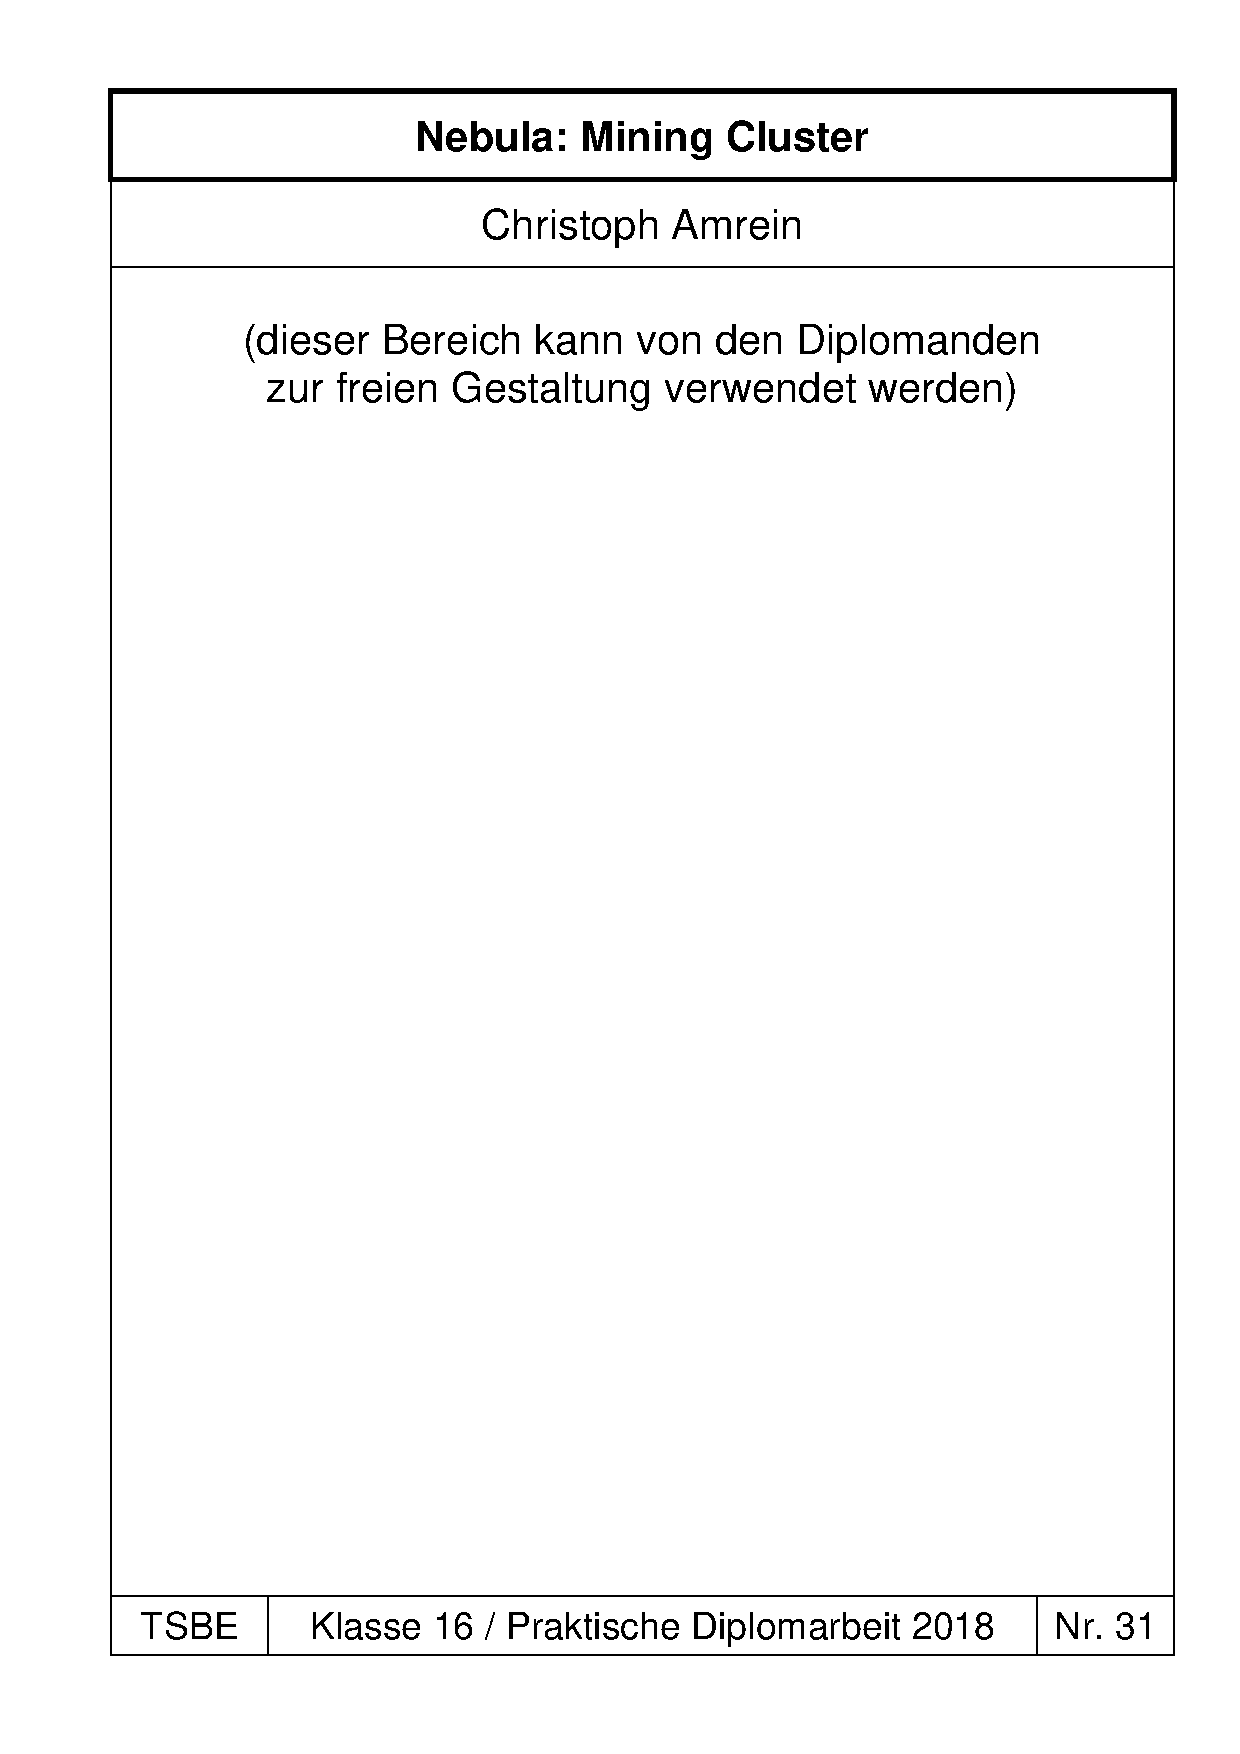
\includepdf[pages=1]{Titelblatt.pdf}
%\Large{Abschlussprüfung \pruefungstermin}\\[3ex]

%\Large{\ausbildungsberuf}\\
%\LARGE{\betreff}\\[4ex]

%\huge{\textbf{\titel}}\\[1.5ex]
%\Large{\textbf{\untertitel}}\\[4ex]

%\normalsize
%Abgabetermin: \abgabeOrt, den \abgabeTermin\\[3em]
%\textbf{Prüfungsbewerber:}\\
%\autorName\\
%\autorAnschrift\\
%\autorOrt\\[5ex]

%\includegraphics[scale=0.4]{\betriebLogo}\\[2ex]
%\textbf{Ausbildungsbetrieb:}\\
%\betriebName\\
%\betriebAnschrift\\
%\betriebOrt\\[5em]
\end{center}
\end{figure}
%\small
%\noindent

\end{titlepage}
\cleardoublepage

% !TEX root = ../Projektdokumentation.tex
\section{Management Summary}
%\label{sec:Management Summary}



% Preface --------------------------------------------------------------------
\phantomsection
\pdfbookmark[1]{Inhaltsverzeichnis}{inhalt}
\tableofcontents
\cleardoublepage


% Inhalt ---------------------------------------------------------------------
\pagenumbering{arabic}
% !TEX root = Projektdokumentation.tex
%% !TEX root = ../Projektdokumentation.tex
\section{Projektplanung} 
\label{sec:Projektplanung}


\subsection{Projektphasen}
\label{sec:Projektphasen}

\begin{itemize}
	\item In welchem Zeitraum und unter welchen Rahmenbedingungen (\zB Tagesarbeitszeit) findet das Projekt statt?
	\item Verfeinerung der Zeitplanung, die bereits im Projektantrag vorgestellt wurde.
\end{itemize}

\paragraph{Beispiel}
Tabelle~\ref{tab:Zeitplanung} zeigt ein Beispiel für eine grobe Zeitplanung.
\tabelle{Zeitplanung}{tab:Zeitplanung}{ZeitplanungKurz}\\
Eine detailliertere Zeitplanung findet sich im \Anhang{app:Zeitplanung}.


\subsection{Abweichungen vom Projektantrag}
\label{sec:AbweichungenProjektantrag}

\begin{itemize}
	\item Sollte es Abweichungen zum Projektantrag geben (\zB Zeitplanung, Inhalt des Projekts, neue Anforderungen), müssen diese explizit aufgeführt und begründet werden.
\end{itemize}


\subsection{Ressourcenplanung}
\label{sec:Ressourcenplanung}

\begin{itemize}
	\item Detaillierte Planung der benötigten Ressourcen (Hard-/Software, Räumlichkeiten \usw).
	\item \Ggfs sind auch personelle Ressourcen einzuplanen (\zB unterstützende Mitarbeiter).
	\item Hinweis: Häufig werden hier Ressourcen vergessen, die als selbstverständlich angesehen werden (\zB PC, Büro). 
\end{itemize}


\subsection{Entwicklungsprozess}
\label{sec:Entwicklungsprozess}
\begin{itemize}
	\item Welcher Entwicklungsprozess wird bei der Bearbeitung des Projekts verfolgt (\zB Wasserfall, agiler Prozess)?
\end{itemize}

%% !TEX root = ../Projektdokumentation.tex
\section{Analysephase} 
\label{sec:Analysephase}


\subsection{Ist-Analyse} 
\label{sec:IstAnalyse}
\begin{itemize}
	\item Wie ist die bisherige Situation (\zB bestehende Programme, Wünsche der Mitarbeiter)?
	\item Was gilt es zu erstellen/verbessern?
\end{itemize}


\subsection{Wirtschaftlichkeitsanalyse}
\label{sec:Wirtschaftlichkeitsanalyse}
\begin{itemize}
	\item Lohnt sich das Projekt für das Unternehmen?
\end{itemize}


\subsubsection{\gqq{Make or Buy}-Entscheidung}
\label{sec:MakeOrBuyEntscheidung}
\begin{itemize}
	\item Gibt es vielleicht schon ein fertiges Produkt, dass alle Anforderungen des Projekts abdeckt?
	\item Wenn ja, wieso wird das Projekt trotzdem umgesetzt?
\end{itemize}


\subsubsection{Projektkosten}
\label{sec:Projektkosten}
\begin{itemize}
	\item Welche Kosten fallen bei der Umsetzung des Projekts im Detail an (\zB Entwicklung, Einführung/Schulung, Wartung)?
\end{itemize}

\paragraph{Beispielrechnung (verkürzt)}
Die Kosten für die Durchführung des Projekts setzen sich sowohl aus Personal-, als auch aus Ressourcenkosten zusammen.
Laut Tarifvertrag verdient ein Auszubildender im dritten Lehrjahr pro Monat \eur{1000} Brutto. 

\begin{eqnarray}
8 \mbox{ h/Tag} \cdot 220 \mbox{ Tage/Jahr} = 1760 \mbox{ h/Jahr}\\
\eur{1000}\mbox{/Monat} \cdot 13,3 \mbox{ Monate/Jahr} = \eur{13300} \mbox{/Jahr}\\
\frac{\eur{13300} \mbox{/Jahr}}{1760 \mbox{ h/Jahr}} \approx \eur{7,56}\mbox{/h}
\end{eqnarray}

Es ergibt sich also ein Stundenlohn von \eur{7,56}. 
Die Durchführungszeit des Projekts beträgt 70 Stunden. Für die Nutzung von Ressourcen\footnote{Räumlichkeiten, Arbeitsplatzrechner etc.} wird 
ein pauschaler Stundensatz von \eur{15} angenommen. Für die anderen Mitarbeiter wird pauschal ein Stundenlohn von \eur{25} angenommen. 
Eine Aufstellung der Kosten befindet sich in Tabelle~\ref{tab:Kostenaufstellung} und sie betragen insgesamt \eur{2739,20}.
\tabelle{Kostenaufstellung}{tab:Kostenaufstellung}{Kostenaufstellung.tex}


\subsubsection{Amortisationsdauer}
\label{sec:Amortisationsdauer}
\begin{itemize}
	\item Welche monetären Vorteile bietet das Projekt (\zB Einsparung von Lizenzkosten, Arbeitszeitersparnis, bessere Usability, Korrektheit)?
	\item Wann hat sich das Projekt amortisiert?
\end{itemize}

\paragraph{Beispielrechnung (verkürzt)}
Bei einer Zeiteinsparung von 10 Minuten am Tag für jeden der 25 Anwender und 220 Arbeitstagen im Jahr ergibt sich eine gesamte Zeiteinsparung von 
\begin{eqnarray}
25 \cdot 220 \mbox{ Tage/Jahr} \cdot 10 \mbox{ min/Tag} = 55000 \mbox{ min/Jahr} \approx 917 \mbox{ h/Jahr} 
\end{eqnarray}

Dadurch ergibt sich eine jährliche Einsparung von 
\begin{eqnarray}
917 \mbox{h} \cdot \eur{(25 + 15)}{\mbox{/h}} = \eur{36680}
\end{eqnarray}

Die Amortisationszeit beträgt also $\frac{\eur{2739,20}}{\eur{36680}\mbox{/Jahr}} \approx 0,07 \mbox{ Jahre} \approx 4 \mbox{ Wochen}$.


\subsection{Nutzwertanalyse}
\label{sec:Nutzwertanalyse}
\begin{itemize}
	\item Darstellung des nicht-monetären Nutzens (\zB Vorher-/Nachher-Vergleich anhand eines Wirtschaftlichkeitskoeffizienten). 
\end{itemize}

\paragraph{Beispiel}
Ein Beispiel für eine Entscheidungsmatrix findet sich in Kapitel~\ref{sec:Architekturdesign}: \nameref{sec:Architekturdesign}.


\subsection{Anwendungsfälle}
\label{sec:Anwendungsfaelle}
\begin{itemize}
	\item Welche Anwendungsfälle soll das Projekt abdecken?
	\item Einer oder mehrere interessante (!) Anwendungsfälle könnten exemplarisch durch ein Aktivitätsdiagramm oder eine \ac{EPK} detailliert beschrieben werden. 
\end{itemize}

\paragraph{Beispiel}
Ein Beispiel für ein Use Case-Diagramm findet sich im \Anhang{app:UseCase}.


\subsection{Qualitätsanforderungen}
\label{sec:Qualitaetsanforderungen}
\begin{itemize}
	\item Welche Qualitätsanforderungen werden an die Anwendung gestellt (\zB hinsichtlich Performance, Usability, Effizienz \etc (siehe \citet{ISO9126}))?
\end{itemize}


\subsection{Lastenheft/Fachkonzept}
\label{sec:Lastenheft}
\begin{itemize}
	\item Auszüge aus dem Lastenheft/Fachkonzept, wenn es im Rahmen des Projekts erstellt wurde.
	\item Mögliche Inhalte: Funktionen des Programms (Muss/Soll/Wunsch), User Stories, Benutzerrollen
\end{itemize}

\paragraph{Beispiel}
Ein Beispiel für ein Lastenheft findet sich im \Anhang{app:Lastenheft}. 

\Zwischenstand{Analysephase}{Analyse}

%% !TEX root = ../Projektdokumentation.tex
\section{Entwurfsphase} 
\label{sec:Entwurfsphase}

\subsection{Zielplattform}
\label{sec:Zielplattform}

\begin{itemize}
	\item Beschreibung der Kriterien zur Auswahl der Zielplattform (\ua Programmiersprache, Datenbank, Client/Server, Hardware).
\end{itemize}


\subsection{Architekturdesign}
\label{sec:Architekturdesign}
\begin{itemize}
	\item Beschreibung und Begründung der gewählten Anwendungsarchitektur (\zB \acs{MVC}).
	\item \Ggfs Bewertung und Auswahl von verwendeten Frameworks sowie \ggfs eine kurze Einführung in die Funktionsweise des verwendeten Frameworks.
\end{itemize}

\paragraph{Beispiel}
Anhand der Entscheidungsmatrix in Tabelle~\ref{tab:Entscheidungsmatrix} wurde für die Implementierung der Anwendung das \acs{PHP}-Framework Symfony\footnote{\Vgl \citet{Symfony}.} ausgewählt. 

\tabelle{Entscheidungsmatrix}{tab:Entscheidungsmatrix}{Nutzwert.tex}


\subsection{Entwurf der Benutzeroberfläche}
\label{sec:Benutzeroberflaeche} 
\begin{itemize}
	\item Entscheidung für die gewählte Benutzeroberfläche (\zB GUI, Webinterface).
	\item Beschreibung des visuellen Entwurfs der konkreten Oberfläche (\zB Mockups, Menüführung).
	\item \Ggfs Erläuterung von angewendeten Richtlinien zur Usability und Verweis auf Corporate Design.
\end{itemize}

\paragraph{Beispiel}
Beispielentwürfe finden sich im \Anhang{app:Entwuerfe}.


\subsection{Datenmodell}
\label{sec:Datenmodell}

\begin{itemize}
	\item Entwurf/Beschreibung der Datenstrukturen (\zB \acs{ERM} und/oder Tabellenmodell, \acs{XML}-Schemas) mit kurzer Beschreibung der wichtigsten (!) verwendeten Entitäten.
\end{itemize}

\paragraph{Beispiel}
In \Abbildung{ER} wird ein \ac{ERM} dargestellt, welches lediglich Entitäten, Relationen und die dazugehörigen Kardinalitäten enthält. 

\begin{figure}[htb]
\centering
\includegraphicsKeepAspectRatio{ERDiagramm.pdf}{0.6}
\caption{Vereinfachtes ER-Modell}
\label{fig:ER}
\end{figure} 


\subsection{Geschäftslogik}
\label{sec:Geschaeftslogik}

\begin{itemize}
	\item Modellierung und Beschreibung der wichtigsten (!) Bereiche der Geschäftslogik (\zB mit Kom\-po\-nen\-ten-, Klassen-, Sequenz-, Datenflussdiagramm, Programmablaufplan, Struktogramm, \ac{EPK}).
	\item Wie wird die erstellte Anwendung in den Arbeitsfluss des Unternehmens integriert?
\end{itemize}

\paragraph{Beispiel}
Ein Klassendiagramm, welches die Klassen der Anwendung und deren Beziehungen untereinander darstellt kann im \Anhang{app:Klassendiagramm} eingesehen werden.

\Abbildung{Modulimport} zeigt den grundsätzlichen Programmablauf beim Einlesen eines Moduls als \ac{EPK}.
\begin{figure}[htb]
\centering
\includegraphicsKeepAspectRatio{modulimport.pdf}{0.9}
\caption{Prozess des Einlesens eines Moduls}
\label{fig:Modulimport}
\end{figure}


\subsection{Maßnahmen zur Qualitätssicherung}
\label{sec:Qualitaetssicherung}
\begin{itemize}
	\item Welche Maßnahmen werden ergriffen, um die Qualität des Projektergebnisses (siehe Kapitel~\ref{sec:Qualitaetsanforderungen}: \nameref{sec:Qualitaetsanforderungen}) zu sichern (\zB automatische Tests, Anwendertests)?
	\item \Ggfs Definition von Testfällen und deren Durchführung (durch Programme/Benutzer).
\end{itemize}


\subsection{Pflichtenheft/Datenverarbeitungskonzept}
\label{sec:Pflichtenheft}
\begin{itemize}
	\item Auszüge aus dem Pflichtenheft/Datenverarbeitungskonzept, wenn es im Rahmen des Projekts erstellt wurde.
\end{itemize}

\paragraph{Beispiel}
Ein Beispiel für das auf dem Lastenheft (siehe Kapitel~\ref{sec:Lastenheft}: \nameref{sec:Lastenheft}) aufbauende Pflichtenheft ist im \Anhang{app:Pflichtenheft} zu finden.


\Zwischenstand{Entwurfsphase}{Entwurf}

%% !TEX root = ../Projektdokumentation.tex
\section{Abnahmephase} 
\label{sec:Abnahmephase}

\begin{itemize}
	\item Welche Tests (\zB Unit-, Integrations-, Systemtests) wurden durchgeführt und welche Ergebnisse haben sie geliefert (\zB Logs von Unit Tests, Testprotokolle der Anwender)?
	\item Wurde die Anwendung offiziell abgenommen?
\end{itemize}

\paragraph{Beispiel}
Ein Auszug eines Unit Tests befindet sich im \Anhang{app:Test}. Dort ist auch der Aufruf des Tests auf der Konsole des Webservers zu sehen.


\Zwischenstand{Abnahmephase}{Abnahme}

%% !TEX root = ../Projektdokumentation.tex
\section{Einführungsphase}
\label{sec:Einfuehrungsphase}

\begin{itemize}
	\item Welche Schritte waren zum Deployment der Anwendung nötig und wie wurden sie durchgeführt (automatisiert/manuell)?
	\item Wurden \ggfs Altdaten migriert und wenn ja, wie?
	\item Wurden Benutzerschulungen durchgeführt und wenn ja, Wie wurden sie vorbereitet?
\end{itemize}


\Zwischenstand{Einführungsphase}{Einfuehrung}

%% !TEX root = ../Projektdokumentation.tex
\section{Dokumentation}
\label{sec:Dokumentation}

\begin{itemize}
	\item Wie wurde die Anwendung für die Benutzer/Administratoren/Entwickler dokumentiert (\zB Benutzerhandbuch, \acs{API}-Dokumentation)?
	\item Hinweis: Je nach Zielgruppe gelten bestimmte Anforderungen für die Dokumentation (\zB keine IT-Fachbegriffe in einer Anwenderdokumentation verwenden, aber auf jeden Fall in einer Dokumentation für den IT-Bereich).
\end{itemize}

\paragraph{Beispiel}
Ein Ausschnitt aus der erstellten Benutzerdokumentation befindet sich im \Anhang{app:BenutzerDoku}.
Die Entwicklerdokumentation wurde mittels PHPDoc\footnote{Vgl. \cite{phpDoc}} automatisch generiert. Ein beispielhafter Auszug aus der Dokumentation einer Klasse findet sich im \Anhang{app:Doc}. 

\Zwischenstand{Dokumentation}{Dokumentation}

%% !TEX root = ../Projektdokumentation.tex
\section{Fazit} 
\label{sec:Fazit}

\subsection{Soll-/Ist-Vergleich}
\label{sec:SollIstVergleich}

\begin{itemize}
	\item Wurde das Projektziel erreicht und wenn nein, warum nicht?
	\item Ist der Auftraggeber mit dem Projektergebnis zufrieden und wenn nein, warum nicht?
	\item Wurde die Projektplanung (Zeit, Kosten, Personal, Sachmittel) eingehalten oder haben sich Abweichungen ergeben und wenn ja, warum?
	\item Hinweis: Die Projektplanung muss nicht strikt eingehalten werden. Vielmehr sind Abweichungen sogar als normal anzusehen. Sie müssen nur vernünftig begründet werden (\zB durch Änderungen an den Anforderungen, unter-/überschätzter Aufwand).
\end{itemize}

\paragraph{Beispiel (verkürzt)}
Wie in Tabelle~\ref{tab:Vergleich} zu erkennen ist, konnte die Zeitplanung bis auf wenige Ausnahmen eingehalten werden.
\tabelle{Soll-/Ist-Vergleich}{tab:Vergleich}{Zeitnachher.tex}


\subsection{Lessons Learned}
\label{sec:LessonsLearned}

\begin{itemize}
	\item Was hat der Prüfling bei der Durchführung des Projekts gelernt (\zB Zeitplanung, Vorteile der eingesetzten Frameworks, Änderungen der Anforderungen)?
\end{itemize}


\subsection{Ausblick}
\label{sec:Ausblick}

\begin{itemize}
	\item Wie wird sich das Projekt in Zukunft weiterentwickeln (\zB geplante Erweiterungen)?
\end{itemize}

% !TEX root = ../Diplombericht.tex
% !TEX root = ../Diplombericht.tex

\section{Ausgangslage}
Die aktuelle Umgebung ist nicht auf das Schürfen von Kryptowährungen ausgelegt. Das System hat eine Uptime von maximal 40\%. Auch der Standort, der Lärm und die Hitze des Systems und Raumes werden als störend empfunden. Dadurch wurden hauptsächlich Tokens auf Börsen gekauft, welche nicht geschürft werden können. Die Sicherung der Daten ist ebenfalls nicht gewährleistet. Zudem existieren keine Monitoring Tools, welche den Status des Schürfens und der Hardware zu erkennen geben. Dabei wird das Analysieren von Problemen als schwierig erachtet, da keine Logdaten existieren, oder diese mit viel Aufwand zusammengesucht werden müssen. Es wurde bereits vor dem Projektstart die benötigte Hardware für die Umsetzung der neuen HPC Cluster Lösung besorgt.


\subsection{Weshalb soll das Projekt realisiert werden?}
Es soll eine stabile Lösung zum Schürfen von Kryptowährungen auf CPU Basis erschaffen werden, welche permanent in Betrieb sein kann und Profit generiert.

\subsection{Für wen ist das Projekt gedacht?}
Das Projekt wird in eigenem Interesse aufgebaut. Es existieren demnach keine Kunden und Abhängigkeiten zu anderen Personen oder Unternehmen.


% !TEX root = ../Diplombericht.tex
\subsection{Situationsanalyse}
Für das Schürfen von Kryptowährungen werden folgende Komponenten eingesetzt:
\begin{table}[H]
\begin{tabular}[t]{p{0.5cm}p{0.8cm}p{6.7cm}p{6.7cm}}
\hline
\rowcolor{heading}\textbf{Nr.} & \textbf{Typ} & \textbf{Komponente} & \textbf{Modell \/Version} \\\hline
1 & HW & Prozessor & Intel Core i7-4700, 3.40 GHz Quad Core \\\hline
2 & HW & Grafikkarte & NVIDIA GeForce GTX 1070 Ti  \\\hline
3 & HW & Festplatte & TOSHIBA DT01ACA200  \\\hline
4 & SW & Schürf-Software & Minergate, Version 7.2  \\\hline
5 & SW & Betriebssystem & Windows 10 EDU, Version 1709 \\\hline
\end{tabular}
\caption{Situationsanalyse Komponenten}
\end{table}


\textbf{Legende:} HW = Hardware, SW = Software

\subsubsection{Stärken}
\begin{table}[H]
\begin{tabular}[t]{p{0.5cm}p{4.1cm}p{10.1cm}}
\hline
\rowcolor{heading}\textbf{Nr.} & \textbf{Kategorie} & \textbf{Beschreibung} \\\hline
1 & Bedienbarkeit & Das Schürfen der Währungen kann über ein Graphical User Interface (GUI) gestartet werden. \\\hline
2 & Wartung & Es existieren keine Umsysteme  \\\hline
\end{tabular}
\caption{Situationsanalyse Stärken}
\end{table}

\subsubsection{Schwächen}
\begin{table}[H]
\begin{tabular}[t]{p{0.5cm}p{4.1cm}p{10.1cm}}
\hline
\rowcolor{heading}\textbf{Nr.} & \textbf{Kategorie} & \textbf{Beschreibung} \\\hline
1 & Flexibilität & Während des Schürfens ist der Computer für andere Tätigkeiten blockiert. \\\hline
2 & Kosten & Die Betriebskosten sind höher als der Ertrag.  \\\hline
3 & Betriebszeit & Es können nicht durchgehend Kryptowährungen geschürft werden.  \\\hline
\end{tabular}
\caption{Situationsanalyse Schwächen}
\end{table}
% !TEX root = ../Diplombericht.tex
\subsection{Ziele}
\subsubsection{Vorgehensziele}

\textbf{Zeitplan}
\newline
Während der Initialisierungsphase wurde eine Projektplanung mit den Aufgaben und den vorgesehenen Aufwänden während des Projektes erstellt. Die definierten Soll-Aufwände sollen mit den stetig nachgeführten IST-Aufwänden verglichen werden. Die Abweichungen werden im Projektplan direkt errechnet.

\textbf{Meilensteine}
\newline
Die Meilensteine wurden in der Zeitplanung des Projektes berücksichtigt und definiert. Die Aufwände werden jeweils im Projektplan nachgeführt, dies ermöglicht einen Ist- und Soll-Aufwand Vergleich

\textbf{Arbeitsjournal}
\newline
Das Arbeitsjournal wird alle 2 Wochen an die Experten versendet. Diese haben die Möglichkeit die Aufwände und investierte Zeit zu prüfen.

\textbf{Beweiserbringung}
\newline
Alle geleisteten Arbeiten sollen in dokumentarischer Form, Präsentation oder einem Gespräch bewiesen werden können.
% !TEX root = ../Diplombericht.tex
\newpage
\subsubsection{Projektziele} 
\label{sec:Projektziele}

\begin{table}[H]
\begin{tabular}[t]{p{0.7cm}p{6.1cm}p{6.1cm} >{\centering}p{0.6cm}c}
\hline
\rowcolor{heading}\textbf{Nr.} & \textbf{Ziel} & \textbf{Messgrösse} & \textbf{Kat.} & \textbf{Prio.} \\\hline
01 & Die CPU des Clusters soll zu 90\% zum Schürfen von Kryptowährung  beansprucht werden. & Log und Monitoring Auswertungen nach dem Testlauf. & LZ & \textbf{M} \\\hline
02 & Die Daten werden auf einem Network Attached Storage (NAS) mit Redundant Array of Independent Disks (RAID I) gesichert. & Die Festplatten werden einzeln überprüft, der Datenbestand muss identisch sein. & BZ \newline TZ & \textbf{M} \\\hline
03 & Der Cluster soll eine Verfügbarkeit von 98\% aufweisen. & Dies kann erst nach dem Testlauf durch ein Monitoring der Laufzeit gemessen werden. & LZ \newline BZ \newline TZ & \textbf{M} \\\hline
04 & Es können während des Betriebs neue Compute Nodes hinzugefügt werden \& ausfallende Compute Nodes verursachen keinen Unterbruch des Betriebs. & Während der Testphase werden neue Compute Nodes hinzugefügt und Compute Nodes vom Cluster getrennt.  & LZ \newline BZ \newline TZ & \textbf{M} \\\hline 
05 & Der Cluster kann für verschiedene Anwendungsgebiete eingesetzt werden. & Während der Testphase werden andere Applikationen, welche die Cluster Ressourcen verwenden sollen, installiert. & BZ & \textbf{M} \\\hline
06 & Das Betriebssystem soll über das Netzwerk an die Compute Nodes verteilt werden, um SD-Karten zu sparen und ein Betriebssystem zentral verwalten zu können. & Wird während der Installation über Systemlogdateien ausgelesen und mit SSH-Zugriffen getestet. & WZ \newline BZ \newline TZ & \textbf{M} \\\hline
07 & Das Schürfprogramm soll automatisch die gewinnbringendste Währung abbauen. & Nach der Testphase werden die Logdateien und Wallets ausgewertet und mit Daten der Währungskurse abgeglichen. & LZ \newline WZ & \textbf{K} \\\hline
08 & Mit der geschürften Währung soll auf Börsen gehandelt werden können. & Kann nach der Realisierung durch Transaktionslogdaten gemessen werden. & LZ \newline WZ & \textbf{K} \\\hline
09 & Die Wartungsarbeiten sollen pro Monat nicht mehr als 3 Stunden betragen. & Wird durch ein Eingriffsprotokoll nach der Realisierungsphase festgehalten. & BZ & \textbf{K} \\\hline
10 & Der Cluster soll einfach transportierbar und wiederaufbaubar sein. & Der Cluster wird nach der Testphase physisch verschoben und neu aufgebaut, dabei wird die Zeit des Wiederaufbaus gemessen. & TZ & \textbf{K}\\\hline
\end{tabular}
\caption{Projektziele}
\end{table}

\textbf{Legende:} LZ = Leistungsziel, WZ = Wirtschaftsziel, BZ = Betriebsziel, TZ = Technisches Ziel, \newline M = Muss-Kriterium, K = Kann-Kriterium

\subsubsection{Lieferobjekte}
Folgende Dokumente werden während des Projektes erstellt und geliefert:

\begin{table}[H]
\begin{tabular}[t]{p{0.5cm}p{6.5cm}p{6.5cm}p{1.8cm}}
\hline
\rowcolor{heading}\textbf{Nr.} & \textbf{Dokument} & \textbf{Phase} & \textbf{Termin} \\\hline
1 & Projektplan & Initialisierung & 15.02.2018 \\\hline
2 & Projektlogo & Initialisierung & 20.02.2018 \\\hline
3 & Projektauftrag & Initialisierung & 20.02.2018 \\\hline
4 & Studie & Initialisierung & 25.02.2018 \\\hline
5 & Detailkonzept & Konzept & 17.03.2018 \\\hline
6 & Testkonzept & Konzept & 22.03.2018 \\\hline
7 & Testprotokoll & Realisierung & 03.05.2018 \\\hline
8 & Installationshandbuch & Realisierung & 10.05.2018 \\\hline
9 & Betriebshandbuch & Realisierung & 13.05.2018 \\\hline
\end{tabular}
\caption{Lieferobjekte}
\end{table}


 

% !TEX root = ../Diplombericht.tex
\subsubsection{Rahmenbedingungen} 
\label{sec:Rahmenbedingungen}

Folgende Bedingungen gelten für die Durchführung des Projektes:
\begin{itemize}
	\item Dem Projekt stehen 294 Stunden Arbeitszeit zur Verügung.
	\item Es wird nach der Projektmethode HERMES gearbeitet.
	\item Der Stundenansatz der involvierten Personen ist auf 120.00 CHF angesetzt.
%	\item Die Hardware wurde bereits vor dem Projekt besorgt.
	\item Neue Anforderungen werden erst nach dem Projektabschluss berücksichtigt.
\end{itemize}

\subsubsection{Abgrenzungen} 
\label{sec:Abgrenzungen}
\begin{itemize}
	\item Das Projekt wird für den privaten Nutzen durchgeführt.
	\item Die Experten sind in den Kostrenrechnungen nicht berücksichtigt.
	\item Der Cluster wird aus Kosten- und Leistungsgründen nicht redundant aufgebaut.
	\item Neue Anforderungen können während des Projektes nicht berücksichtigt werden.
	\item Das Projektbudget kann aus finanziellen Gründen nicht erhöht werden.
	\item Defekte Computenodes werden während des Projektes nicht ersetzt.
\end{itemize}
% !TEX root = ../Diplombericht.tex

\subsection{Lösungsbeschreibung}
Es wird physisch ein Cluster aus mindestens 40 aktiven RPI's aufgebaut. Der Cluster soll aus finanziellen Gründen mit möglichst wenigen Komponenten wie, Netzteile, USB Kabel \& Speicherkarten in Betrieb genommen werden. Dabei wird das Betriebssystem zentral verwaltet und über das Netzwerk an die einzelnen Raspberry PI's verteilt. Zugleich wird zur Datensicherheit ein Netzwerkshare (NAS) mit RAID I installiert. Zusätzlich soll die rentabelste Währung automatisch für eine Woche geschürft werden, bevor eine erneute Prüfung auf die rentabelste Währung geschieht. Die geschürften Kryptowährungen werden jeweils in die entsprechenden verschlüsselten Wallets transferiert. Durch die geschürften Währungen soll an Börsen gehandelt werden können, welche es ermöglichen sollen Profit zu erzielen. Durch eine Monitoring, Alarming und Logdaten Lösung soll auf Missstände des Clusters aufmerksam gemacht werden. Die Tools bieten sich sogleich für eine Analyse der Probleme an und sind über einen Webbrowser aufrufbar.   
% !TEX root = ../Diplombericht.tex

\subsection{Kosten}

\subsubsection{Einmalige Kosten}
\textbf{Beschaffungskosten}
\begin{table}[H]
\centering
\begin{tabular}{p{2cm}p{5cm}p{4cm}p{4cm}}
\hline
\rowcolor{heading} \textbf{Anzahl} & \textbf{Komponente} & \hfill \textbf{Stückpreis(CHF)} & \hfill \textbf{Gesamtwert(CHF)} \\\hline
40 & Raspberry PI Model B & \hfill 33.00 & \hfill 1'320.00 \\\hline
1 & Schaltnetzteil & \hfill  229.00 & \hfill 229.00 \\\hline
1 & TTL Serial Kabel & \hfill 30.00 & \hfill 30.00 \\\hline
40 & Patchkabel Cat. 5e & \hfill 1.00 & \hfill 40.00 \\\hline
1 & TP-Link Switch & \hfill 220.00 & \hfill 220.00 \\\hline
1 & Synology NAS DS216 & \hfill 600.00 & \hfill 600.00 \\\hline
1 & Diverse Kabel, Schrauben & \hfill 50.00 & \hfill 50.00 \\\hline
\rowcolor{subheading}\textbf{-} & \textbf{Total} & \hfill \textbf{-} & \hfill \textbf{2'489.00} \\\hline
\end{tabular}
\caption{Beschaffungskosten}
\end{table}

\textbf{Aufwandskosten}
\begin{table}[H]
\centering
\begin{tabular}{p{2cm}p{5cm}p{4cm}p{4cm}}
\hline
\rowcolor{heading} \textbf{Stunden} & \textbf{Phase} & \textbf{Stundenansatz(CHF)} &\hfill \textbf{Gesamtkosten(CHF)} \\\hline
30 & Initialisierung & \hfill 120.00 & \hfill 3'600.00 \\\hline
41 & Konzept & \hfill 120.00 & \hfill  6'000.00 \\\hline
171 & Realisierung & \hfill 120.00 & \hfill  17'040.00 \\\hline
25.5 & Einführung & \hfill 120.00 & \hfill 2'640.00 \\\hline
25 & Periodische Arbeiten & \hfill 120.00 & \hfill  3'000.00 \\\hline
1.5 & Reserve / Administration & \hfill 120.00 & \hfill 3'000.00 \\\hline
\rowcolor{subheading}\textbf{294} & \textbf{Total} &\hfill  \textbf{120.00} & \hfill \textbf{35'280.00} \\\hline
\end{tabular}
\caption{Aufwandskosten}
\end{table}

\subsubsection{Betriebskosten (repetitiv)}

Folgende Voraussetzungen sind für die folgenden Berechnungen definiert:
\begin{itemize}
	\item 1000 Watt die Stunde kostet 0.2894 CHF
	\item Ein Monat hat 30 Tage
	\item Ein Jahr hat 360 Tage
\end{itemize}

\textbf{Wartungskosten}
\newline
Pro Monat sind 3 Stunden Wartungsaufwand einzuberechnen, dadurch ergeben sich mit dem definierten Stundenansatz jährliche Wartungskosten von \textbf{4'320.00 CHF}. \newline
\newline
\textbf{Stromkosten}\newline
Der Strom wird durch die BKW über den Vertrag Energy Blue bezogen.

\begin{table}[H]
\centering
\begin{tabular}{p{1.5cm}p{2cm}|p{2.75cm}p{2.75cm}p{2.75cm}p{2.75cm}}
\hline
\rowcolor{heading} \textbf{Anzahl} & \textbf{Leistung} & \multicolumn{4}{l}{\textbf{Kosten in CHF}} \\\hline
\rowcolor{subheading} \textbf{RPI} & \textbf{kW} & \textbf{Stunde} &\textbf{Tag} & \textbf{Monat} &\textbf{Jahr} \\\hline
40 & 0.4 & 0.11576 & 2.78 & 83.35 & 1'000.20 \\\hline
\end{tabular}
\caption{Stromkostenrechnung}
\end{table}

\subsubsection{Gesamtkosten}

\textbf{Jährliche Kosten} \newline
Das Projekt wird Anfang Juni abgeschlossen sein. Deshalb belaufen sich die Wartungs- und Stromkosten im 1. Jahr auf die Hälfte gegenüber den Folgejahren.
Der Cluster soll innerhalb von 3 Jahren gewinnbringend wirken. Die jährlichen sowie täglichen Kosten (in CHF) sind der nachfolgenden Tabelle zu entnehmen: 

\begin{table}[H]
\centering
\begin{tabular}{p{4cm}p{4cm}p{4cm}p{4cm}}
\hline
\rowcolor{heading} \textbf{Kostengrund} & \hfill \textbf{Kosten 1. Jahr} & \hfill\textbf{Kosten 2. Jahr} & \hfill \textbf{Kosten 3. Jahr}\\\hline
Beschaffung & \hfill 2'489.00 &\hfill - &\hfill - \\\hline
Aufwand & \hfill 35'280.00 & \hfill- & \hfill- \\\hline
Wartungskosten & \hfill 2'160.00 & \hfill 4'320.00 & \hfill 4'320.00 \\\hline
Stromkosten & \hfill 500.00 & \hfill 1'000.00 & \hfill 1'000.00 \\\hline
\rowcolor{subheading}\textbf{Total} & \hfill \textbf{40'429.00} & \hfill \textbf{45'749.00} & \hfill \textbf{51'069.00} \\\hline
\end{tabular}
\caption{Gesamtkosten}
\end{table}

\textbf{Tägliche Kosten}\newline
Auf 3 Jahre ausgerechnet, muss täglich ein Ertrag von 47.29 CHF erwirtschaftet werden, um die investierten Aufwände und Kosten zu decken.


% !TEX root = ../Diplombericht.tex

\section{Wirtschaftlichkeit}
\subsection{Spekulation}

Der Cluster soll täglich \textbf{30 CHF} erwirtschaften.

Daraus ergibt sich ein tägliches Defizit von -17.36 CHF, welches durch Handeln an Börsen gedeckt werden soll. Durch den volatilen Markt ist es durchaus möglich die \textbf{36.65\%} durch das Handeln zu decken.

\subsection{Infrastruktur}
Es wurde darauf geachtet, dass die Komponenten durch eine zentrale Stelle versorgt werden. Dabei werden die Raspberry PI's mit nur einem Netzteil versorgt und das Betriebssystem wird über das Netzwerk verteilt welches Speicherkarten einspart.

\begin{table}[H]
\centering
\begin{tabular}{p{2cm}p{5cm}p{4cm}p{4cm}}
\hline
\rowcolor{heading} \textbf{Anzahl} & \textbf{Komponente} & \textbf{Stückpreis in CHF} &\textbf{Gesamtwert in CHF} \\\hline
\rowcolor{subheading}\multicolumn{3}{l}{\textbf{Standardlösung}} & \textbf{700.00} \\\hline
4 & USB-HUB 10 Ports & 35.00 & 140.00 \\\hline
40 & Mini-USB Kabel & 6.00 & 240.00 \\\hline
40 & MicroSD Karte & 8.00 & 320.00 \\\hline
\rowcolor{subheading}\multicolumn{3}{l}{\textbf{Projektlösung}} & \textbf{268.00} \\\hline
1 & Netzteil & 230.00 & 230.00 \\\hline
1 & MicroSD Karte & 8.00 & 8.00 \\\hline
- & Diverse Stromkabel & 30.00 & 30.00 \\\hline
\rowcolor{subheading}\multicolumn{3}{l}{\textbf{Differenz der Lösungen}} & \cellcolor{asparagus}\textbf{432.00} \\\hline
\end{tabular}
\caption{Wirtschaftlichkeit Hardware}
\end{table}

Durch die vorgesehene Hardwarelösung können 432.00 CHF eingespart werden. Dies entspricht einer Einsparung von \textbf{261\%}.

\subsection{Return of Investment}


% !TEX root = ../Projektdokumentation.tex
\newpage
\subsection{Planung} 
%\label{sec:Terminplan}
\subsubsection{Grober Projektplan}
Die folgende Tabelle zeigt die Arbeiten an, welche während des Projektes erledigt werden sollen. Ein grafischer und detailierter Projektplan ist über das eingerichtete Confluence\footnote{\url{http://wiki.influ.ch/download/attachments/327735/NEBULA-Projektplan-v1.xlsx?api=v2}} zugänglich.

\begin{table}[H]
\centering
\begin{tabular}{|p{0.7cm}p{6.8cm}p{2cm}p{2cm}|c|c|c|}

%\rowcolor{heading}\textbf{Phase: Vorarbeiten} & \textbf{Von} & \textbf{Bis} & \textbf{Soll} \\\hline
%Ablage erstellen & 05.02.2018 & 05.02.2018 & 0.2 \\\hline
%Projektinitialisierungsauftrag schreiben & 05.02.2018 & 05.02.2018 & 3 \\\hline
%Kickoff-Meeting & 05.02.2018 & 05.02.2018 & 5 \\\hline
\hline
\rowcolor{heading}\multicolumn{2}{l}{\textbf{Aufgabe}} & \textbf{Start} & \textbf{Ende} & \multicolumn{3}{c|}{\textbf{Dauer in Stunden}} \\\cline{5-7} 
\rowcolor{heading}& & & & \textbf{Soll} & \textbf{Ist} & \textbf{Abw.} \\\hline
\rowcolor{subheading} 0.0 & \textbf{Initialisierung} & & & 30 & 38.5 & +8.5\\\hline
0.1 & Projektplan erstellen & 06.02.2018 & 15.02.2018  & 4 & 6 & +2 \\\hline
0.2 & Projektlogo erstellen & 06.02.2018 & 20.02.2018 & 2 & 0.5 & -0.5\\\hline
0.3 & Studie: durchführen   & 06.02.2018 & 20.02.2018 & 18 & 24 & +6\\\hline
0.4 & Projektauftrag erstellen & 20.02.2018 & 25.02.2018 & 2 & 4 & +2\\\hline
0.5 & Diplombericht erstellen  & 25.02.2018 & 28.02.2018 & 4 & 4 & 0\\\hline
\rowcolor{subheading} 1.0 &\textbf{Konzept} & & & 41 & 38.5 & -2.5 \\\hline
1.1 & Zwischen-Meeting & 01.03.2018 & 01.03.2018 & 6 & 5.5 & -0.5\\\hline
1.2 & Detailkonzept erstellen & 05.03.2018 & 17.03.2018 & 12 & 18 & +6\\\hline
1.3 & Testkonzept erstellen & 18.03.2018 & 22.03.2018 & 11 & 12 & +1\\\hline
1.4 & Dokumenten Review & 24.03.2018 & 26.03.2018  & 12 & 3 & -9 \\\hline
\hline
\rowcolor{subheading} 2.0 & \textbf{Realisierung} & & & 171 & 176 & +5\\\hline
2.1 & Physischer Aufbau & 03.04.2018 & 07.04.2018 & 20 & 32 & +12 \\\hline
2.2 & Stromversorgung einrichten & 08.04.2018 & 09.04.2018 & 8 & 7 & -1 \\\hline
2.3 & Raspberry PI's vorbereiten & 17.04.2018 & 17.04.2018 & 4 & 6 & +2 \\\hline
2.4 & Netzwerkboot einrichten & 21.04.2018 & 23.04.2018 & 25 & 25 & 0 \\\hline
2.5 & Cluster Software installieren & 24.04.2018 & 25.04.2018 & 25 & 20 & -5 \\\hline
2.6 & Schürf Software installieren & 26.04.2018 & 26.04.2018 & 12 & 10 & -2 \\\hline
2.7 & Entwickeln von Tools und Automatismen & 02.04.2018 & 28.04.2018 & 30 & 17 &  -13 \\\hline
2.8 & Monitoring einrichten & 01.05.2018 & 10.05.2018 & 14 & 7 & -7\\\hline
2.9 & Periodische Systemtests & 10.04.2018 & 13.05.2018 & 7 & 30 & +13\\\hline
3.0 & Installationshandbuch erstellen & 02.04.2018 & 10.05.2018 & 8 & 10 & +2  \\\hline
3.1 & Testprotokoll erstellen & 02.05.2018 & 03.05.2018 & 9 & 9 & 0 \\\hline
3.2 & Betriebshandbuch & 01.05.2018 & 13.05.2018 & 9 & 3 & -6\\\hline
3.3 & Freigabe zur Einführung & 07.05.2018 & 15.05.2018 & 0 & 0 & 0 \\\hline
\rowcolor{subheading} 4.0 & \textbf{Einführung} & & & 25.5 & 27 & +1.5 \\\hline
4.1 & Abschlussbericht & 17.05.2018 & 22.05.2018 & 9.5 & 15 & +5.5 \\\hline
4.2 & Management Summary & 20.05.2018 & 24.05.2018 & 8 & 2 & -6 \\\hline
4.3 & Vorbereitung  Abschluss Meeting & 22.05.2018 & 27.05.2018 & 3 & 5 & +2 \\\hline
4.4 & Drucken und Binden & 24.05.2018 & 01.06.2018 & 2 & 2 & 0 \\\hline
4.5 & Abschluss-Meeting & 02.06.2018 & 02.06.2018 & 2 & 2 & 0 \\\hline
4.6 & Projektabschluss & 03.06.2018 & 03.06.2018 & 1 & 1 & 0 \\\hline
\end{tabular}
\caption{Grober Projektplan}
\end{table}

\subsubsection{Termine}
\begin{table}[H]
\centering
\begin{tabular}{p{5cm}p{2.4cm}p{4.5cm}p{3.5cm}}
\hline
\rowcolor{heading} \textbf{Ereignis} & \textbf{Datum} & \textbf{Teilnehmer} &\textbf{Standort} \\\hline
\rowcolor{subheading}\multicolumn{4}{l}{\textbf{Einmalige Ereignisse}} \\\hline
Kick-Off Meeting & 05.02.2018 & Projektleiter \& Experten & Post IT, Zollikofen \\\hline
Zwischenmeeting & 01.03.2018 &  Projektleiter \& Experten & GIBB (TSBE), Bern \\\hline
Abgabe des Diplomberichts & 01.06.2018 & Projektleiter & -  \\\hline
Abschlussmeeting & 07.06.2018 & Projektleiter \& Experten & GIBB (TSBE), Bern  \\\hline
\rowcolor{subheading}\multicolumn{4}{l}{\textbf{Periodische Ereignisse}} \\\hline
Statusbericht & Monatlich & Projektleiter & - \\\hline
Arbeitsjournal & 2-Wöchentlich & Projektleiter & -  \\\hline
\end{tabular}
\caption{Termine}
\end{table}
% !TEX root = ../Projektdokumentation.tex
\subsection{Ressourcen}

\subsubsection{Personal}
Kann dem Kapitel Organisation entnommen werden.

\subsubsection{Budget}
Dem privaten Projekt steht ein Budget von 3'750 CHF zu. Die Aufwände werden hierbei nicht berücksichtigt, das keine Löhne bezahlt werden müssen.
\begin{table}[H]
\centering
\begin{tabular}[t]{p{1cm}p{5cm}p{2cm}}
\hline
\rowcolor{heading}\textbf{Nr.} & \textbf{Verwendungszweck} & \textbf{Budget \newline in CHF} \\\hline
1 & Beschaffungen & 3'000 \\\hline
1 & Apéro & 150 \\\hline
2 & Drucken \& Binden & 100 \\\hline
3 & Reserve Kontingent & 500 \\\hline
\textbf{} & \textbf{Total} & \textbf{3'750}  \\\hline
\end{tabular}
\caption{Projektbudget}
\end{table}

\subsubsection{Sachmittel}
Die aufgelisteten Komponenten werden für die Lösung benötigt.


\begin{table}[H]
\centering
\begin{tabular}[t]{p{1cm}p{1.2cm}p{6.5cm}p{6.5cm}}
\hline
\rowcolor{heading}\textbf{Nr.} & \textbf{Anzahl} & \textbf{Komponenten} & Modell / Spezifikationen\\\hline
1 & 40 & Mini Computer & Raspberry PI 3 Model B+\\\hline
2 & 1 & Schaltnetzteil & RSP-750-5, Mean Well\\\hline
3 & 1 & Midi Tower & Corsair Crystal 570X RGB\\\hline
4 & 1 & USB zu TTL Serial-Kabel & Adafruit USB zu TTL Seriel Kabel, 75cm (Kabel) \\\hline
5 & 40 & Ethernetkabel & FTP Cat.5e Patchkabel \\\hline
6 & 1 & Switch & TL-SL3452 48-Port 10/100, TP-Link \\\hline
7 & 1 & Datenspeicher & Synology NAS DS218\\\hline
8 & * & Diverses, Kabel, Distanzbolzen, \newline Kabelschuhe & *\\\hline
\end{tabular}
\caption{Sachmittel}
\end{table}
* Anzahl und Hertseller unbekannt. Die Artikel wurden in lokalen Baumärkten eingekauft
% !TEX root = ../Projektdokumentation.tex
\subsection{Organisation}
\subsubsection{Projektorganisation}
Die Projektorganisation ist wie folgt aufgebaut:

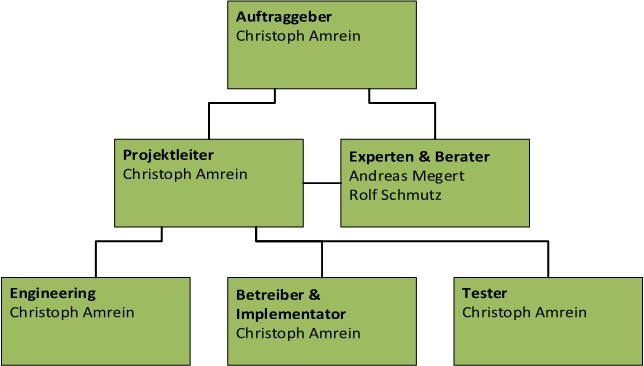
\includegraphics[scale=0.9]{Bilder/Projektorganisation.jpg}{\centering}

\begin{table}[H]
\centering
\begin{tabular}{p{2.5cm}p{13.5cm}}
\hline
\rowcolor{heading}\textbf{Rolle} & \textbf{Verantwortlichkeit} \\\hline
Auftraggeber & Erstellt den Auftrag und übergibt diesen an den Projektleiter \\\hline
Projektleiter & Organisiert die Planung, Durchführung und präsentiert das Projekt \\\hline
Experte & Stehen in Kontakt mit dem Projektleiter und beraten ihn bei Schwierigkeiten \\\hline
Engineering & Stellt dem Betreiber zu implementierende Applikationen zur Verfügung \\\hline
Betreiber & Setzt die Lösung technisch um \\\hline
Tester & Testet die Lösung auf Fehler  \\\hline
\end{tabular}
\caption{Organisation}
\end{table}

\subsubsection{Projektablage}
\begin{table}[H]
\centering
\begin{tabular}{p{1cm}p{4cm}p{11cm}}
\hline
\rowcolor{heading}\textbf{Nr.} & \textbf{Was} & \textbf{Wo} \\\hline
1 & Allgemeine Ablage& wiki.influ.ch \\\hline
2 & Dokumentation & https://github.com/amreinch/Nebula\_AMC \\\hline
3 & Snapshots & Lokal, D:\textbackslash Diplomarbeit\textbackslash CentOS\_works \\\hline
4 & Skripte, Entwürfe & https://github.com/amreinch/OpenHPC\_Install\_Nebula \\\hline
\end{tabular}
\caption{Projektablage}
\end{table}

% !TEX root = ../Diplombericht.tex
\subsection{Cluster-Software Evaluation}
\subsubsection{Cluster Software Kriterien}
Es wurden drei Cluster Software Produkte evaluiert. Dabei mussten die Muss-Kriterien erfüllt werden, um in die Auswahl zu kommen. Diese Kriterien werden für den Entscheid der Software nicht berücksichtigt, grenzen aber die Auswahlmöglichkeit der Produkte ein.

\begin{table}[H]
\begin{tabular}[t]{p{0.7cm}|p{14cm}c}
\hline
\rowcolor{heading}\textbf{Nr.} & \textbf{Anforderung} & \textbf{Prio.} \\\hline
01 & Ist die Software High-Performance-Computing (HPC) tauglich? & M \\\hline
02 & Kann das Produkt innerhalb des vorgesehenen Zeitraumes installiert werden? & M \\\hline
03 & Ist die Lösung skalierbar? &  M \\\hline
04 & Existieren Dokumentationen? & S \\\hline
05 & Kann Support beansprucht und bezogen werden? & S \\\hline
06 & Ist die Lösung benutzerfreundlich? & S \\\hline
07 & Existieren Verwaltungstools? & S \\\hline
08 & Fallen zusätzliche Kosten an? & S \\\hline
\end{tabular}
\caption{Software Kriterien}
\end{table}

\subsubsection{Informationsbeschaffung}
Es wurde nach einer Lösung gemäss der oben definierten Kriterien gesucht. Dabei bin ich auf einen Wikipedia Eintrag\footnote{\url{https://en.wikipedia.org/wiki/Comparison\_of\_cluster\_software}} gestossen, welcher die verschiedenen Cluster Software Angebote auflistet. Dabei wurde nur nach einer HPC Lösung gefiltert. Durch diese Analyse hat sich die OpenHPC Lösung der Linux Foundation herauskristalisiert. Weiterhin wurden Suchbegriffe wie \grqq HPC Raspberry PI\grqq \ über Suchmaschinen eingegeben, da die Compute Nodes des Clusters Raspberry PI's sein sollen. Den Artikel über TinyTitan\footnote{\url{http://www.hpctoday.com/best-practices/tinytitan-a-raspberry-pi-computing-based-cluster/}} habe ich als interessant erachtet und deshalb genauer untersucht.
Mit einer weiteren Suche (hpc cluster software raspberry) bin ich auf einen Guide\footnote{\url{http://thundaxsoftware.blogspot.ch/2016/07/creating-raspberry-pi-3-cluster.html}} gestossen, der relativ simpel aussieht und einfach umzusetzen ist. Es gab durchaus noch weitere Guides und Softwarelösungen, welche ich aber nach einer genaueren Analyse der Installationsanleitung verworfen habe, da diese mir zum Teil zu wenig Informationen lieferten. Während der Informationsbeschaffung wurden alle Installationsskripte und Anleitungen sorgfältig durchgelesen, um diese als mögliche Varianten zu empfehlen. Während der Informationsbeschaffung bin ich auf zwei Fachbegriffe Message Passing Interface (MPI) \& Simple Linux Utility for Resource Management (SLURM), welche meistens in Zusammenhang mit HPC stehen, gestossen. Diese musste ich ebenfalls noch in Erfahrung bringen.






% !TEX root = ../Diplombericht.tex

\subsection{Lösungsvarianten}
\subsubsection{Variantenübersicht}

Die Informationen wurden über die folgenden Produkte gesammelt und zusammengestellt:

\begin{table}[H]
\centering
\begin{tabular}{p{1cm}p{4cm}p{11cm}}
\hline
\rowcolor{heading} \textbf{Nr.} & \textbf{Variante} & \textbf{Bezeichnung} \\\hline
01 & OpenHPC & HPC Lösung entwickelt von der Linux Foundation \\\hline
02 & TinyTitan & Open Source Lösung entwickelt von Oak Ridge Leadership Computing Facility \\\hline
03 & Minimale Lösung & Simple 32-Bit Architekturlösung \\\hline
\end{tabular}
\caption{Variantenübersicht}
\end{table}

\subsubsection{Variante V1 \flqq OpenHPC\frqq}

\textbf{Beschreibung}\newline
OpenHPC gilt als vorangeschrittenes OpenSource Projekt der Linux Foundation. Das Produkt steht in direkter Verbindung mit diversen grossen IT Unternehmen weltweit. Das Ziel der Linux Foundation ist es, durch OpenHPC eine kostengünstige sowie schnell zu installierende HPC-Umgebung aufzubauen. Durch viele zusätzliche OpenSource Tools rundet sich das Produkt ab und gilt als ernstzunehmender Konkurrent gegenüber kostenpflichtiger Software.

\textbf{Installation und Betrieb}\newline
Es existieren diverse Guides, Foren und Chats sowie eine E-Mail-Liste zu OpenHPC. Dadurch scheint die Unterstützung bei allfälligen Problemen vorhanden zu sein. Die Installationsanleitung, welche von der Linux Foundation geschrieben wurde, liest sich sehr gut und ist absolut ausreichend für die Installation. Der Betriebsaufwand wird als gering eingeschätzt, da es ein sehr ausgereiftes Produkt, welches stetig weiterentwickelt wird, ist.

\textbf{Voraussetzungen, Abhängigkeiten}\newline
Für die Cluster Software werden mindestens ein Masternode und 4 Computenodes vorausgesetzt. Das Betriebssystem bezieht sich hierbei auf ein CentOS7x. Jeder Computenode benötigt 2 Netzwerkschnittstellen. Das eine Interface wird für den Standard Ethernet Zugriff verwendet und das zweite Interface wird für die Kommunikation zu jedem BMC Host verwendet. Es werden zusätzliche Intel Bibliotheken benötigt. Dazu müssen Lizenzen für Parallel Studio XE von Intel besorgt werden. Die Lizenzen können mit einer offiziellen E-Mail-Adresse der Schule gratis bezogen werden. Die Linux Foundation erwähnt in ihrem Guide, dass sie die «Bring your own Licence» Strategie verfolgt.

\subsubsection{Variante V2 \flqq TinyTitan\frqq}
\textbf{Beschreibung}\newline
Das Produkt wurde von der Firma «Oak Ridge Facility» entwickelt. Die Software ist unter anderem für RPI’s entwickelt worden. TinyTitan wurde für das Durchführen wissenschaftlicher Berechnungen entworfen. Jedoch wurde seit geraumer Zeit an dem Produkt nicht mehr weitergearbeitet, wie dem offiziellen GitHub Repository zu entnehmen ist. Die Community selbst erweist sich ebenfalls als sehr klein. 

\textbf{Installation und Betrieb}\newline
Für die Installation des Produktes wird ein XServer vorausgesetzt, da empfohlen wird Tiny-Titan über ein GUI zu installieren. Der Installationsanleitung ist ebenfalls zu entnehmen, dass sich die Entwickler viele Gedanken über das Look a Like des Clusters gemacht haben, zum Beispiel wird ein Thema dem Einbinden von LED’s gewidmet. Die Installation findet ausschliesslich durch vordefinierte Scripts statt. Durch die kleine Community und nicht mehr gepflegte Software kann nichts über den Betriebsaufwand in Erfahrung gebracht werden.

\textbf{Voraussetzungen, Abhängigkeiten}\newline
Laut Guides werden lediglich 2 RPI’s benötigt.

\subsubsection{Variante V3 \flqq Minimale Lösung\frqq}
\textbf{Beschreibung}\newline
Die Minimale Installation ist eine zum Teil Eigenbau Lösung, welche sich nahe an diverse Guides aus dem Internet bezieht. Jedoch wird diese auf eigene Bedürfnisse angepasst.

\textbf{Installation und Betrieb}\newline
Da es bei dieser Lösung selber zu entscheiden gilt, was und wie die Lösung installiert und umgesetzt werden soll, kann während der Installation darauf geachtet werden, was den grössten Vorteil für den Betrieb danach mit sich bringt. Während dem Projekt soll die Installation aber klein gehalten werden und nur das nötigste wird umgesetzt. 

\textbf{Voraussetzungen, Abhängigkeiten}\newline
Es werden 2 RPI's benötigt.

\subsubsection{Anforderungsabdeckung der Varianten}

\begin{table}[H]
\centering
\begin{tabular}{p{1cm}p{2.5cm}p{2.2cm}p{10.3cm}}
\hline
\rowcolor{heading} \textbf{Nr.} & \textbf{Kriterium} & \textbf{Gewichtung} &\textbf{Begründung} \\\hline
1 & Installation & 40\% & Die Installation soll keine Hürden aufweisen, da der Zeitplan ansonsten nicht eingehalten werden kann. \\\hline
2 & Partner & 10\% & Je mehr Partner vorhanden sind, desto grösser und innovativer ist die Software. Die Software hat dadurch einen fixen Standpunkt auf dem Markt und wird weiterentwickelt. \\\hline
3 & Aktualität & 20\% & Fördert den LifeCycle und die Sicherheit der Cluster-Software. \\\hline
4 & Tools & 30\% & Mitgelieferte Tools. \\\hline
\end{tabular}
\caption{Anforderungsabdeckung}
\end{table}

\subsubsection{Notenskala der Kriterien}
\begin{table}[H]
\centering
\begin{tabular}{p{0.6cm}p{2.2cm}p{1.cm}p{12.2cm}}
\hline
\rowcolor{heading} \textbf{Nr.} & \textbf{Kriterium} & \textbf{Note} &\textbf{Begründung} \\\hline
1 & Installation & 0/3/5 & 5 = Kann gemäss Anleitung direkt installiert werden. \newline 3 = Veraltete Anleitung. Komplikationsprobleme möglich. \newline
0 = Keine Anleitung vorhanden.
 \\\hline
2 & Partner & 0/2 & 2 = Viele Partner vorhanden. \newline
0 = Keine Partner vorhanden \\\hline
3 & Aktualität & 0/3/5 & 5 = Releases in den letzten 2 Monaten. \newline 3 = Releases in den letzten 6 Monaten \newline 0 = Keine Releases seit einem Jahr. \\\hline
4 & Tools & 0/5 & 5 = Es werden Tools angeboten \newline 0 = Es werden keine Tools angeboten. \\\hline
\end{tabular}
\caption{Notenskala der Kriterien}
\end{table}

\subsection{Bewertung der Varianten}
\begin{table}[H]
\centering
\begin{tabular}{p{2cm}p{2cm}p{4cm}p{4cm}p{4cm}}
\hline
\rowcolor{heading} \textbf{Kriterium} & \textbf{Gewicht} & \textbf{Variante 1} & \textbf{Variante 2}& \textbf{Variante 3} \\\hline
Installation & 40\% & 5x40 = 200 & 4x40 = 160 & 5x40 = 200 \\\hline
Partner & 10\% & 2x10 = 20 & 0x10 = 0 & 0x10 = 0 \\\hline
Aktualität & 20\% & 5x20 = 100 & 0x20 = 0 & 5x20 = 100 \\\hline
Tools & 30\% & 5x30 = 150 & 0x30 = 0 & 0x30 = 0\\\hline
\textbf{Total} & \textbf{100\%} & \ \ \ \ \ \ \ \ \ \ \ \textbf{470} & \ \ \ \ \ \ \ \ \ \ \textbf{160} & \ \ \ \ \ \ \ \ \ \ \ \textbf{300} \\\hline
\end{tabular}
\caption{Bewertung der Varianten}
\end{table}

\subsection{Variantenentscheid}
Anhand der Bewertung wird empfohlen, die OpenHPC Lösung der Linux Foundation zu verwenden. Die Installation kann gemäss Anleitung in kürzester Zeit umgesetzt werden. Die Releases können mit kleinerem Aufwand installiert werden. Zudem runden die Möglichkeiten der Schnittstellen und Komponenten den Entscheid ab. Es ist möglich, Administrations- sowie Performance Monitoring Tools einzusetzen, welche mit der Lösung harmonieren. Als Hürde sehe ich die möglichen anfallenden Lizenzen und das zweite Netzwerk Interface, welches man für die Kommunikation unter den RPI’s benötigt.
% !TEX root = ../Diplombericht.tex

\section{Lösungsvarianten}
\subsection{Variantenübersicht}

Die Informationen wurden über die folgenden Produkte gesammelt und zusammengestellt:

\begin{table}[H]
\centering
\begin{tabular}{p{1cm}p{4cm}p{11cm}}
\hline
\rowcolor{heading} \textbf{Nr.} & \textbf{Variante} & \textbf{Bezeichnung} \\\hline
01 & OpenHPC & HPC Lösung entwickelt von der Linux Foundation \\\hline
02 & TinyTitan & Open Source Lösung entwickelt von Oak Ridge Leadership Computing Facility \\\hline
03 & Minimale Lösung & Simple 32-Bit Architekturlösung \\\hline
\end{tabular}
\caption{Variantenübersicht}
\end{table}

\subsection{Variante V1 \flqq OpenHPC\frqq}

\subsubsection{Beschreibung}
OpenHPC gilt als vorangeschrittenes OpenSource Projekt der Linux Foundation. Das Produkt steht in direkter Verbindung mit diversen grossen IT Unternehmen weltweit. Das Ziel der Linux Foundation ist es, durch OpenHPC eine kostengünstige sowie schnell zu installierende HPC-Umgebung aufzubauen. Durch viele zusätzliche OpenSource Tools rundet sich das Produkt ab und gilt als ernstzunehmender Konkurrent gegenüber kostenpflichtiger Software.

\subsubsection{Installation und Betrieb}
Es existieren diverse Guides, Foren und Chats sowie eine E-Mail-Liste zu OpenHPC. Dadurch scheint die Unterstützung bei allfälligen Problemen vorhanden zu sein. Die Installati-onsanleitung, welche von der Linux Foundation geschrieben wurde, liest sich sehr gut und ist absolut ausreichend für die Installation. Der Betriebsaufwand wird als gering eingeschätzt, da es ein sehr ausgereiftes Produkt, welches stetig weiterentwickelt wird, ist.

\subsubsection{Voraussetzungen, Abhängigkeiten}
Für die Cluster Software werden mindestens ein Masternode und 4 Computenodes voraus-gesetzt. Das Betriebssystem bezieht sich hierbei auf ein CentOS7x. Jeder Computenode be-nötigt 2 Netzwerkschnittstellen. Das eine Interface wird für den Standard Ethernet Zugriff verwendet und das zweite Interface wird für die Kommunikation zu jedem BMC Host ver-wendet. Es werden zusätzliche Intel Bibliotheken benötigt. Dazu müssen Lizenzen für Parallel Studio XE von Intel besorgt werden. Die Lizenzen können mit einer offiziellen E-Mail-Adresse der Schule gratis bezogen werden. Die Linux Foundation erwähnt in ihrem Guide, dass sie die «Bring your own Licence» Strategie verfolgt.

\subsection{Variante V2 \flqq TinyTitan\frqq}
\subsubsection{Beschreibung}
Das Produkt wurde von der Firma «Oak Ridge Facility» entwickelt. Die Software ist unter anderem für RPI’s entwickelt worden. TinyTitan wurde für das Durchführen wissenschaftli-cher Berechnungen entworfen. Jedoch wurde seit geraumer Zeit an dem Produkt nicht mehr weitergearbeitet, wie dem offiziellen GitHub Repository zu entnehmen ist. Die Community selbst erweist sich ebenfalls als sehr klein. 

\subsubsection{Installation und Betrieb}
Für die Installation des Produktes wird ein XServer vorausgesetzt, da empfohlen wird Tiny-Titan über ein GUI zu installieren. Der Installationsanleitung ist ebenfalls zu entnehmen, dass sich die Entwickler viele Gedanken über das Look a Like des Clusters gemacht haben, zum Beispiel wird ein Thema dem Einbinden von LED’s gewidmet. Die Installation findet aus-schliesslich durch vordefinierte Scripts statt. Durch die kleine Community und nicht mehr ge-pflegte Software kann nichts über den Betriebsaufwand in Erfahrung gebracht werden.

\subsubsection{Voraussetzungen, Abhängigkeiten}
Laut Guides werden lediglich 2 RPI’s benötigt.

\subsection{Variante V3 \flqq Minimale Lösung\frqq}
\subsubsection{Beschreibung}
Die Minimale Installation ist eine zum Teil Eigenbau Lösung, welche sich nahe an diverse Guides aus dem Internet bezieht. Jedoch wird diese auf eigene Bedürfnisse angepasst.

\subsubsection{Installation und Betrieb}
Da es bei dieser Lösung selber zu entscheiden gibt, was und wie die Lösung installiert und umgesetzt werden soll, kann während der Installation darauf geachtet werden, was den grössten Vorteil für den Betrieb danach mit sich bringt. Während dem Projekt soll die Installation aber klein gehalten werden und nur das nötigste wird umgesetzt. 

\subsubsection{Voraussetzungen, Abhängigkeiten}
Es werden 2 RPI's benötigt.

% !TEX root = ../Projektdokumentation.tex
\section{Studie} 
\label{sec:Studie}
Hier werden Grundsatzentscheide gefällt, es werden keine Details beschrieben!
\begin{itemize}
	\item Informationsbeschaffung
	\item Anforderungskatalog
	\item Schwachstellenkatalog
	\item Pflichtenheft
	\item Analyse welche Varianten möglich sind
	\item Evaluation der möglichen Varianten
	\item Entscheid mit welcher Varianten das Konzept realisiert wird
	\item Wirtschaftlichkeit
\end{itemize}


\subsection{Informationsbeschaffung}
Durch die Studie soll eine HPC Cluster Software Lösung welche mit Raspberry PI's kompatibel ist evaluiert werden.

\subsubsection{Informationsbeschaffung}
Es wurden über den Wikipedia Eintrag \hyperref[Wikipedia Eintrag]{https://en.wikipedia.org/wiki/Comparison\_of\_cluster\_software} die verschiedenen Cluster Software Angebote verglichen. Dabei wurde nur nach einer HPC Lösung gefiltert. Die Anforderungen an die Cluster Software ist, dass es eine gratis Lösung sein muss, zudem ist ein komplett Paket erwünscht und nicht nur eine minimale Softwarelösung. Durch diese Analyse hat sich die OpenHPC Lösung der Linux Foundation herauskristalisiert. Weiterhin wurden Suchbegriffe wie "HPC Raspberry PI" über Suchmaschinen im Internet eingegeben da die Computenodes des Cluster Raspberry PI's sein sollen. Folgender Artikel habe ich als interessant erachtet und wurde analysiert.\hyperref[TinyTitan]{http://www.hpctoday.com/best-practices/tinytitan-a-raspberry-pi-computing-based-cluster/}
Mit einer weiteren Suche(hpc cluster software raspberry) bin ich auf einen Guide gestossen, der relativ simpel aussieht und einfach umzusetzen ist.\hyperref[Eigenbau]{http://thundaxsoftware.blogspot.ch/2016/07/creating-raspberry-pi-3-cluster.html}. Es gab durchaus noch weitere Guides und Softwarelösungen, welche ich aber nach einer genaueren Installationsanleitung verworfen habe, da diese mir zum Teil zu wenig Informationen lieferten. Während der Informationsbeschaffung wurden alle Installationsskripte und Anleitungen sorgfältig durchgelesen um diese als mögliche Variante zu empfehlen.

\subsubsection{Anforderungskatalog}
Es wurden folgende Anforderungen an die Cluster Software gestellt.

\begin{itemize}
\item Die Software soll auf einer 64 Bit Architektur betrieben werden können.
\item Es müssen stabile Releases vorhanden sein
\item Die Software soll eine skalierbare Funktion beinhalten.
\item Die Software soll die CPU Ressourcen für Berechnungsaufgaben zu mindestens 90\% auslasten.
\item Es sollen Monitoring Tools bereits in der Softwarelösung vorhanden sein
\item Es sollen Logging Tools bereits in der Softwarelösung vorhanden sein
\item Die Softwarelösung soll mit einem Netzwerkboot zurecht kommen.
\item Die Software muss gratis sein.
\item Die Installation soll einfach und nachvollziehbar sein.
\item Es sollen mehrere Befehlssatzarchitekturen unterstützt werden.
\item Die Softwarelösung soll eine Community für Fragen anbieten.
\item Der Letzte Release soll nicht lange zurückliegen.
\item Die Software soll bereits einen bekanntheitsgrad vorweisen.
\end{itemize}




% !TEX root = ../Diplombericht.tex
\newpage
\section{Konzept} 
\label{sec:Konzept}
Das Konzept beschreibt den vorgesehenen Aufbau des Clusters und beinhaltet die Testfälle, welche bei der Abnahme nach der Realisierung berücksichtigt werden müssen.

% !TEX root = ../Diplombericht.tex
\subsection{Physikalischer Überblick}
Die nachfolgende Abbildung stellt ein verinfachter Überblick der vorgesehenen Infratstruktur dar.

\begin{figure}[htb]
\centering
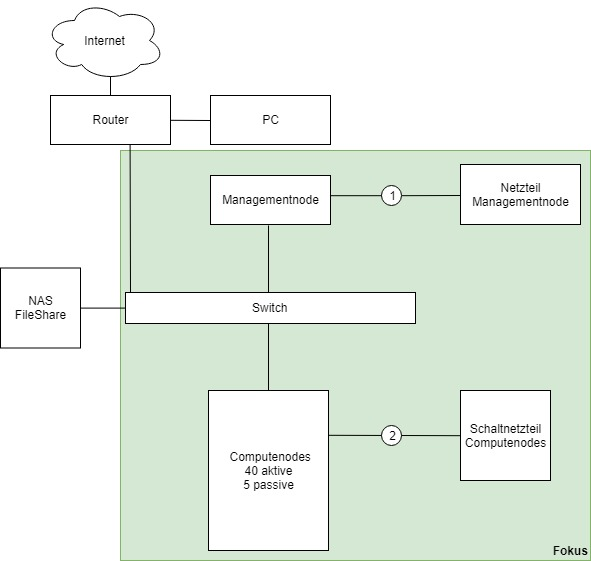
\includegraphics[scale=0.5]{phys_ueberblick.jpg}
\caption{Physikalischer Überblick}
\label{fig:Physikalischer Überblick}
\end{figure} 

\textbf{Beschreibung}\newline
Der grün markierte Teil beinhaltet das Vorhaben. Diese Komponenten werden neu in das Netzwerk eingebunden und aufgebaut. Die Komponenten ausserhalb des grünen Bereiches existieren bereits und es müssen für die Umsetzung konfigurationen vorgenommen werden.

\textbf{Verbindung 1} \newline
Der Managementnode wird über ein herkömmliches Netzteil per Micro USB mit Stom versorgt.

\textbf{Verbindung 2} \newline
Die Computenodes werden über ein Schaltnetzteil über die GPIO Pins mit Stom betrieben.



% !TEX root = ../Diplombericht.tex
\subsection{Physikalische Verbindungen}

\subsubsection{Stromversorgung Management Node}
Der Management Node wird über den Micro USB Anschluss mit Strom versorgt. Dabei muss darauf geachtet werden, dass ein mindest Strom von 2 Ampere fliesst. Zudem wird eine konstante Spannung von 5 Volt benötigt. Deshalb wird ein Netzteil mit einer Leistung von 10 Watt verwendet. Das Netzteil wird über eine Stromschiene an das Stromnetz angeschlossen.

\subsubsection{Compute Nodes}
Die Compute Nodes werden über die GPIO Pins via Jumperkabel über ein gemeinsames Netzteil mit Strom versorgt. Da es sich hierbei um eine Anzahl von mindestens 45 Raspberry's handelt, ist ein Netzteil mit einer Leistung von 500W vorgesehen. Das Netzteil wird über die Stromschiene an das Stomnetz angeschlossen.


\subsubsection{Übrige Geräte}
Die übrigen Geräte werden über den herkömmlichen Weg mit Strom über eine Stromschiene versorgt.

\subsubsection{Netzwerkverbindungen}
Die folgenden Komponenten sind über den Switch in das lokale Netzwerk eingebunden. Die nicht aufgelisteten Geräte werden direkt über Powerline oder WLAN mit dem Router verbunden:
\begin{itemize}
\item Management Node
\item Compute Nodes
\item NAS
\end{itemize}



% !TEX root = ../Diplombericht.tex
\subsection{Technischer Überblick}
\begin{figure}[H]
\centering
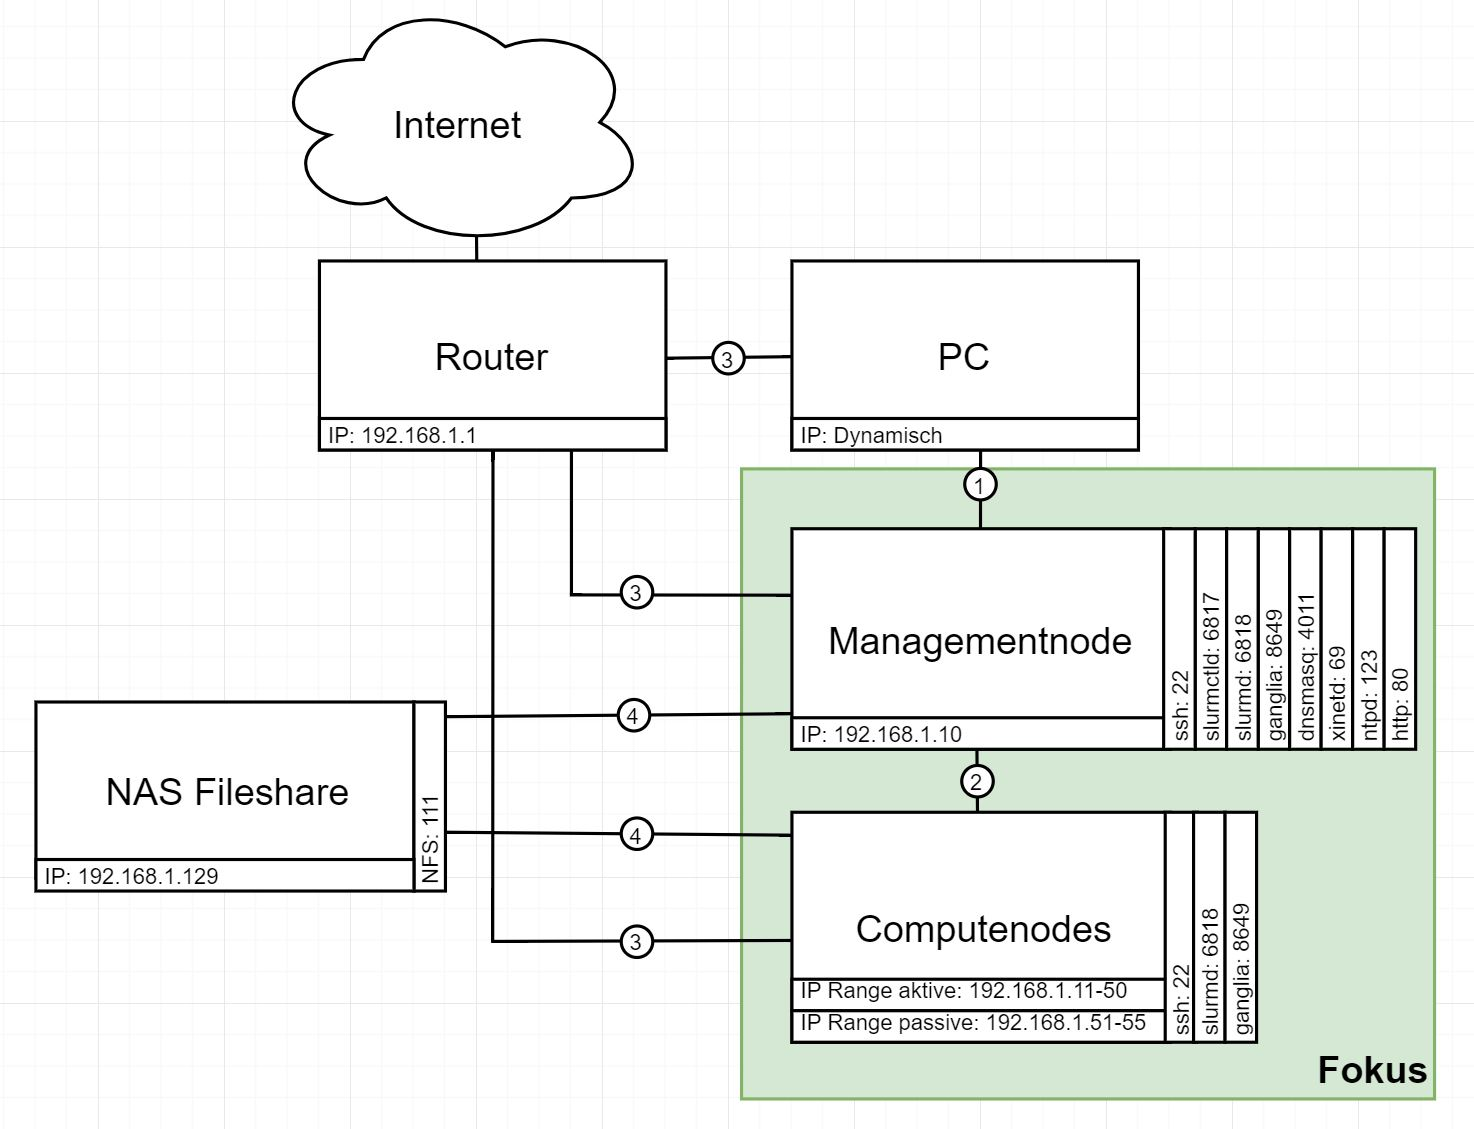
\includegraphics[scale=0.5]{tech_ueberblick.jpg}
\caption{Technischer Überblick}
\label{fig:Technischer Überblick}
\end{figure} 

\textbf{Beschreibung}\newline
Der grün markierte Teil beinhaltet das Vorhaben. Diese Komponenten werden neu in das Netzwerk eingebunden und aufgebaut. Die Komponenten ausserhalb des grünen Bereiches existieren bereits und es müssen für die Umsetzung konfigurationen vorgenommen werden.

\textbf{Verbindung 1} \newline
Der PC kann mit dem \textbf{SSH Protokoll} auf den Managementnode zugreifen. Dadurch kann die Installation vorgenommen werden. Zugleich wird über \textbf{HTTP} via Webbrowser der Zugriff auf diverse Applikationen wie z.B. Nagios \& Ganglia ermöglicht.

\textbf{Verbindung 2} \newline
Der Managementnode verteilt via \textbf{dnsmasq} und  \textbf {TFTP} das Betriebssystem an die Computenodes über das Netzwerk. Sogleich ist auch der \textbf{Slurm Controller} für die Jobsteuerung auf dem Managementnode installiert, welcher mit den \textbf{Slurm Daemons} auf den Computenodes kommuniziert. Weiterhin sind die Monitoring Komponenten \textbf{Ganglia und Nagios} auf dem Managementnode installiert, welche Monitoringdaten der Computenodes sammeln und zur Auswertung verarbeiten.

\textbf{Verbindung 3} \newline
Der Router verteilt via \textbf{DHCP} statische IP Adressen und Hostnamen welche über die MAC Adressen definiert sind.

\textbf{Verbindung 4} \newline
Der NAS Share wird über \textbf{SMB} auf den Computenodes und dem Masternode angehängt.

\subsubsection{Verwendete Protokolle}
\begin{table}[H]
\centering
\begin{tabular}{p{2cm}p{4cm}p{5cm}p{5cm}}
\hline
\rowcolor{heading} \textbf{Verbindung} & \textbf{Protokoll} & \textbf{Protokollfamilie} & \textbf{Ports} \\\hline
1 & SSH & TCP & 22 \\\hline
2 & SMTP & TCP & 25 \\\hline
3 & DHCP & UDP & 67 / 78 \\\hline
4 & TFTP & UDP & 69 \\\hline
5 & HTTP & TCP & 80 \\\hline
6 & SMB & TCP & 445 \\\hline
\end{tabular}
\caption{Protokolle}
\end{table}

% !TEX root = ../Diplombericht.tex
\subsection{Technische Verbindungen \& Kommunikation}
\begin{table}[H]
\centering
\begin{tabular}{p{1cm}p{1.5cm}p{1.5cm}p{2.2cm}p{8.8cm}}
\hline
\rowcolor{heading} \textbf{Nr.} & \textbf{Quelle} & \textbf{Ziel }& \textbf{Betrifft} & \textbf{Beschreibung} \\\hline
1 & NAS & Mgmt & Datenablage & Der NAS Share wird über das NFS Protkoll angehängt. \\\hline
2 & NAS & Compute & Datenablage & Der NAS Share wird über das NFS Protkoll angehängt. \\\hline
3 & Router & Mgmt & IP Adresse & Anhand der MAC Adresse wird eine statische IP Adresse zugewiesen. \\\hline
4 & Router & Compute & IP Adressen & Anhand der MAC Adressen werden statische IP Adressen zugewiesen. \\\hline
5 & Router & Mgmt &Hostname & Es wird über den Router ein definierter Hostname verteilt. \\\hline
6 & Router & Compute & Hostnamen & Es werden über den Router definierte Hostnamen verteilt. \\\hline
7 & Mgmt & Compute & Netzwerkboot & Der Management Node beliefert die Compute Nodes über das TFT Protokoll mit dem Betriebssystem \\\hline
8 & Internet & Mgmt & Zeitserver & Die aktuelle Zeit wird mit NTP über das Internet synchronisiert.\\\hline
9 & Mgmt & Compute & Zeitserver & Die Compute Nodes beziehen die aktuelle Zeit über NTP.\\\hline
10 & Internet & Compute & Internetzugriff & Die Compute Nodes können über ein Routing über den Mgmt auf das Internet zugreifen. \\\hline
11 & PC & Mgmt & Zugriff & Verbindungen über den PC können mit dem SSH Protokoll aufgebaut werden. \\\hline
12 & PC & Compute & Zugriff & Verbindungen über den PC können mit dem SSH Protokoll aufgebaut werden. \\\hline
\end{tabular}
\caption{Verbindungen \& Kommunikation}
\end{table}
\textbf{Legende:} Mgmt = Management Node, Compute = Compute Nodes, PC = Home Computer

% !TEX root = ../Diplombericht.tex
\subsection{Komponentenbeschreibung}
\subsubsection{Router}

Bei dem Router handelt es sich um eine Internet-Box Plus von Swisscom. Das Admin Interface ist über http://internetbox aufrufbar.

\subsubsection{PC}
Der PC ist selbst zusammengestellt und wird nur für Webzugriffe auf Applikationen welche auf dem Managementnode laufen verwendet. Zusätzlich wird per SSH auf den Managementnode zugegriffen.

\subsubsection{Managementnode}
Der Managementnode dient der Jobsteuerung sowie Clusterverwaltung. Alle zentralen Programme sind auf diesem Node installiert.

\begin{table}[H]
\centering
\begin{tabular}{|l|l|}
\hline
Hostname & nebula \\\hline
Modell & Raspberry PI 3 \\\hline
Betriebssystem & Centos 7.4 \\\hline
Architektur & 64 Bit \\\hline
\end{tabular}
\caption{Komponente Managementnode}
\end{table}

\subsubsection{Netzteil Managementnode}
Das Netzteil liefert eine konstante Spannung von 5V und Strom von mindestens 2 Ampere. Dabei handelt es sich um ein Noname Netzeil welches eine Mindestleistug von 10 Watt aufbringen muss.

\subsubsection{NAS}
Das NAS ist von der Firma Synology, das Modell lautet DS216 und wird als redundanter Datenspeicher benutzt.

\subsubsection{Switch}
Der Managed Switch TL-SL3428 von TP-Link wird für die Kommunikation zwischen NAS, Managementnode und den Computenodes benötigt. Auf die Managed Funktion wird allerdings während des Aufbaus und Betriebs verzichtet.

\subsubsection{Computenodes}
Die Computenodes erhalten über das Netzwerk das Betriebssystem durch den Managementnode zugestellt. Dabei sind alle Hostnamen mit dem Prefix "c" versehen und werden aufnummeriert. Dabei sind die Computenodes in aktiv und passiv (Fallback, Reserve) aufgeteilt, die passiven Computenodes sollen ausgefallene aktive Computenodes ersetzen und deren Arbeiten und Leistung übernehmen.

\textbf{Aktiv}
\begin{table}[H]
\centering
\begin{tabular}{|l|l|}
\hline
Hostname & c[1-40] \\\hline
Modell & Raspberry PI 3 \\\hline
Betriebssystem & Centos 7.4 \\\hline
Architektur & 64 Bit \\\hline
\end{tabular}
\caption{Komponente aktive Copmputenodes}
\end{table}

\textbf{Passiv}
\begin{table}[H]
\centering
\begin{tabular}{|l|l|}
\hline
Hostname & c[41-45] \\\hline
Modell & Raspberry PI 3 \\\hline
Betriebssystem & Centos 7.4 \\\hline
Architektur & 64 Bit \\\hline
\end{tabular}
\caption{Komponente passive Copmputenodes}
\end{table}

\subsubsection{Schaltnetzteil Computenodes}
Das Schaltnetzteil RSP-750-5 von Mean Well liefert konstante 5 Volt aus Ausgangsspannung und kann eine Leistung bis zu 500 Watt aufbringen.


% !TEX root = ../Diplombericht.tex
\subsection{Tests}
\subsubsection{Testobjekte}
Die folgende Hardware ist für die Tests der Funktionsfähigkeit des Clusters im Scope vorgesehen:
\begin{table}[H]
\centering
\begin{tabular}{p{1cm}p{7.cm}p{7.5cm}}
\hline
\rowcolor{heading} \textbf{Nr.} & \textbf{Objekt} & \textbf{Beschreibung} \\\hline
1 & Management Node & Raspberry PI 3  \\\hline
2 & Compute Nodes & Raspberry PI 3 \\\hline
3 & NAS & Synology NAS DS216 \\\hline
4 & Switch & TP-Link TL-SL3428 \\\hline
\end{tabular}
\caption{Testobjekte}
\end{table}

\subsubsection{Testarten}
Die Tests werden in folgende Kategorien eingestuft:

\begin{table}[H]
\centering
\begin{tabular}{p{1cm}p{3cm}p{12cm}}
\hline
\rowcolor{heading} \textbf{Nr.} & \textbf{Testart} & \textbf{Beschreibung} \\\hline
1 & Komponententest & Die Lauffähigkeit und Erreichbarkeit der einzelnen Hardware Komponenten wird überprüft.  \\\hline
2 & Integrationstest & Es wird die Zusammenarbeit der aktiven und neu integrierten abhängigen Komponenten überprüft. \\\hline
3 & Systemtest & Das System wird als Komplettlösung getestet. Hierbei soll geprüft werden, ob die Lösung den Anforderungen der Anwendbarkeit und Nutzbarkeit dem Auftrag entspricht.  \\\hline
\end{tabular}
\caption{Testarten}
\end{table}

\subsubsection{Testvoraussetzungen}
\textbf{Startbedingungen}\newline
Für den Start der Tests muss der Cluster aufgebaut sein und die einzelnen Komponenten müssen mit Strom versorgt sein. 

\textbf{Abbruchbedingungen}\newline
Die Tests werden abgebrochen, sobald Fehler auftauchen, welche Folgetests verhindern.

\subsubsection{Fehlerklassen}
\begin{table}[H]
\centering
\begin{tabular}{p{1cm}p{4cm}p{11cm}}
\hline
\rowcolor{heading} \textbf{Nr.} & \textbf{Fehlerklassen} & \textbf{Beschreibung} \\\hline
1 & Fehlerfrei & Die Erwartungen sind erfüllt.  \\\hline
2 & Harmloser Mangel & Es sind keine Betriebsverhinderungen zu erkennen. Die Erwartungen sind erfüllt. \\\hline
3 & Kleiner Mangel & Der Betrieb kann aufgenommen werden. Das Problem sollte aber über einen Zeitraum von 6 Monaten behoben werden.  \\\hline
4 & Schwerer Mangel & Der Cluster kann nur teilweise in Betrieb genommen werden. Der Mangel muss innerhalb zwei Wochen behoben werden. \\\hline
5 & Kritischer Mangel & Der Cluster kann nicht in Betrieb genommen werden. Die Mängel müssen umgehend behoben werden. \\\hline
\end{tabular}
\caption{Fehlerklassen}
\end{table}

\subsubsection{Testhilfsmittel}
Die Dokumentation der Tests wird im Testprotokoll nachgeführt. Damit die Tests durchgeführt werden können wird ein PC oder Notebook als Testclient benötigt. Dieser Client muss sich im selben Netzwerk wie der Cluster befinden.


% !TEX root = ../Diplombericht.tex
\subsection{Monitoring}
Es werden zwei Überwachungsapplikationen eingesetzt, welche über einen Browser aufrufbar sind. Dabei wird zwischen Service- und Performancemonitoring unterschieden.

\subsubsection{Service Monitoring}
Als Servicemonitoring wird die Applikation Nagios eingesetzt. Alle Abfragen auf sämtliche Nodes finden automatisiert vom Managementnode aus statt. Sämtliche Fehler werden per E-Mail gemeldet. Adresse gemeldetDabei müssen folgende Überwachungen implementiert werden.

\begin{table}[H]
\begin{tabular}[t]{p{0.6cm}p{2.5cm}p{2.2cm}p{1.5cm}p{8.8cm}}
\hline
\rowcolor{heading}\textbf{Nr.} & \textbf{Überwachung} & \textbf{Schweregrad} & \textbf{Intervall} &\textbf{Beschreibung} \\\hline
1 & Erreichbarkeit & Kritisch & 5 & Es wird mittels Ping eine Statusüberprüfung der Nodes durchgeführt \\\hline
2 & SSH Zugriff & Mittel & 60 & Die Zugriffe auf die Computenodes sollen über den Managementnode stattfinden  \\\hline
3 & CPU Last & Hoch & 5 & Die CPU's ständig ausgelastet sein  \\\hline
\end{tabular}
\caption{Service Monitoring}
\end{table}

\textbf{Meldungen \& Alarme} \newline
Sobald sich der Status einer Überwachung ändert, wird eine Nachricht per E-Mail an den Systemadministrator gesendet.





% !TEX root = ../Diplombericht.tex
\subsection{Mining}
Die Kryptowährungen werden über die Miningpools von Minergate.com geschürft. Dafür wird die cpuminer Version von tkinjo1985 verwendet. Diese Version unterstützt die ARMv8 Prozessoren und bietet alle gängigen Algorithmen für das Schürfen der Währungen an.
Zudem werden nur Währungen geschürft, welche auf Börsen resp. Märkten gehandelt werden können.


\subsubsection{Kryptowährungen}
Folgende Kryptowährungen werden über die Minergate Pools mit dem CryptoNight Algorithmus geschürft:

\begin{table}[H]
\centering
\begin{tabular}{p{1cm}p{3.5cm}p{2cm}p{9.5cm}}
\hline
\rowcolor{heading} \textbf{Nr.} & \textbf{Währung} & \textbf{Kürzel} &\textbf{Märkte } \\\hline
1 & Bytecoin & BCN & HitBTC, Poloniex \\\hline
2 & Monero & XMR & HitBTC, Binance, Bitfinex, Poloniex \\\hline
3 & Monero Original & XMO & HitBTC \\\hline
4 & DigitalNote & XDN & HitBTC, Bittrex \\\hline
5 & Quazar Coin & QCN & HitBTC \\\hline
6 & DashCoin & DSH & HitBTC \\\hline
7 & FantomCoin & FCN & HitBTC \\\hline
\end{tabular}
\caption{Kryptowährungen}
\end{table}


\subsection{Automatisiertes Schürfen}
Das zu entwickelnde Skript, welches automatisch die gewinnbringendste Kryptowährung schürfen soll, muss per Curl auf  die API von Coinmarketcap\footnote{\url{https://api.coinmarketcap.com/}} der jeweiligen Währung zugreifen. Dabei soll die Antwort für das Ermitteln der gewinnbringendsten Währung dienen.
% !TEX root = ../Diplombericht.tex
\subsection{Hostnamen}
Die Compute Node Namen wurden nach einem überschaulichen Konzept definiert. Jeder Compute Node trägt den Prefix "c". Dies soll bei der Behebung von Problemen auf physicher Ebene, z.B. Austauschen eines Nodes, dienen. Zudem werden alle Hostnamen immer in kleinen Buchstaben geschrieben. 

\subsubsection{Management Node Name}
\begin{table}[H]
\centering
\begin{tabular}{p{5cm}p{5.5cm}p{5.5cm}}
\hline
\rowcolor{heading} \textbf{Name} & \textbf{IP} & \textbf{MAC} \\\hline
nebula & 192.168.1.10 & B8:27:EB:32:A9:1C \\\hline
\end{tabular}
\caption{Management Node Name}
\end{table}

\subsubsection{Compute Node Namen}
\begin{longtable}{p{1cm}p{2cm}p{6cm}p{6cm}}
\hline
\rowcolor{heading} \textbf{Nr.} & \textbf{Name} & \textbf{IP} & \textbf{MAC} \\\hline
01 & c1 & 192.168.1.11 & B8:27:EB:32:39:A7\\\hline
02 & c2 & 192.168.1.12 & B8:27:EB:2E:A3:D1\\\hline
03 & c3 & 192.168.1.13 & B8:27:EB:50:45:3F\\\hline
04 & c4 & 192.168.1.14 & B8:27:EB:0D:E6:25\\\hline
05 & c5 & 192.168.1.15 & B8:27:EB:3E:96:B5\\\hline
06 & c6 & 192.168.1.16 & B8:27:EB:EE:77:DA\\\hline
07 & c7 & 192.168.1.17 & B8:27:EB:21:63:E6\\\hline
08 & c8 & 192.168.1.18 & B8:27:EB:2E:2E:CC\\\hline
09 & c9 & 192.168.1.19 & B8:27:EB:17:32:96\\\hline
10 & c10 & 192.168.1.20 & B8:27:EB:B2:1C:A9\\\hline
11 & c11 & 192.168.1.21 & B8:27:EB:AF:63:1F\\\hline
12 & c12 & 192.168.1.22 & B8:27:EB:43:00:2C\\\hline
13 & c13 & 192.168.1.23 & B8:27:EB:13:7B:18\\\hline
14 & c14 & 192.168.1.24 & B8:27:EB:43:CD:29\\\hline
15 & c15 & 192.168.1.25 & B8:27:EB:FF:C7:56\\\hline
16 & c16 & 192.168.1.26 & B8:27:EB:CE:98:66\\\hline
17 & c17 & 192.168.1.27 & B8:27:EB:5D:63:34\\\hline
18 & c18 & 192.168.1.28 & B8:27:EB:91:3E:0F\\\hline
19 & c19 & 192.168.1.29 & B8:27:EB:F4:65:EC\\\hline
20 & c20 & 192.168.1.30 & B8:27:EB:3E:AB:DC\\\hline
21 & c21 & 192.168.1.31 & B8:27:EB:66:60:F6\\\hline
22 & c22 & 192.168.1.32 & B8:27:EB:37:3F:74\\\hline
23 & c23 & 192.168.1.33 & B8:27:EB:18:5E:F0\\\hline
24 & c24 & 192.168.1.34 & B8:27:EB:B0:23:B8\\\hline
25 & c25 & 192.168.1.35 & B8:27:EB:BE:C4:94\\\hline
26 & c26 & 192.168.1.36 & B8:27:EB:FB:FF:57\\\hline
27 & c27 & 192.168.1.37 & B8:27:EB:4E:EC:CE\\\hline
28 & c28 & 192.168.1.38 & B8:27:EB:43:1C:35\\\hline
29 & c29 & 192.168.1.39 & B8:27:EB:DC:74:5F\\\hline
30 & c30 & 192.168.1.40 & B8:27:EB:D1:DE:2F\\\hline
31 & c31 & 192.168.1.41 & B8:27:EB:5E:90:34\\\hline
32 & c32 & 192.168.1.42 & B8:27:EB:DE:80:24\\\hline
33 & c33 & 192.168.1.43 & B8:27:EB:A4:79:6F\\\hline
34 & c34 & 192.168.1.44 & B8:27:EB:0A:4D:C7\\\hline
35 & c35 & 192.168.1.45 & B8:27:EB:5C:53:5F\\\hline
36 & c36 & 192.168.1.46 & B8:27:EB:F7:AF:C2\\\hline
37 & c37 & 192.168.1.47 & B8:27:EB:CE:BA:ED\\\hline
38 & c38 & 192.168.1.48 & B8:27:EB:59:38:3C\\\hline
39 & c39 & 192.168.1.49 & B8:27:EB:99:BB:8E\\\hline
40 & c40 & 192.168.1.50 & B8:27:EB:8F:7A:0D\\\hline
\caption{Compute Node Namen}
\end{longtable}


\subsubsection{Reserve Node Name}
Die Reservenodes sind als Fallback für ausgefallene Compute Nodes vorgesehen.
\begin{table}[H]
\centering
\begin{tabular}{p{1cm}p{2cm}p{6cm}p{6cm}}
\hline
\rowcolor{heading} \textbf{Nr.} & \textbf{Name} & \textbf{IP} & \textbf{MAC} \\\hline
1 & c41 & 192.168.1.51 & B8:27:EB:DE:C9:69 \\\hline
2 & c42 & 192.168.1.52 & B8:27:EB:7E:6F:48 \\\hline
3 & c43 & 192.168.1.53 & B8:27:EB:5D:DD:FE \\\hline
4 & c44 & 192.168.1.54 & B8:27:EB:A6:6D:4D \\\hline
5 & c45 & 192.168.1.55 & B8:27:EB:0C:63:10 \\\hline
\end{tabular}
\caption{Reserve Node Namen}
\end{table}
% !TEX root = ../Projektdokumentation.tex
\section{Realisierung und Einführung} 
\label{sec:RealisierungEinfuehrung}

\begin{itemize}
	\item Schlusskommentar zum Ergebnis der gesamten Arbeit
	\item Wie geht es weiter mit dem Projekt
	\item Persönliche Betrachtung
	\item Danksagung
	\item Urheberrecht
\end{itemize}

\subsection{Ausführen}
\begin{itemize}
	\item Lösungen ausarbeiten
	\item Prototyp erstellen
\end{itemize}

\subsection{Tests}
\begin{itemize}
	\item Planung
	\begin{itemize}
		\item Was wird getestet
		\item Welche Tests sollen durchgeführt werden?
		\item Welches Resultat wird erwartet
	\end{itemize}
	\item Durchführung
	\item Auswertung, Testbericht
	\item Protokollierung (wie wurde getestet): Die Testanordnung muss ersichtlich sein.
	Das Test-Quipment (Geräte, div. Material) muss erfasst und aufgelistet werden.
	Tests müssen immer nachvollziehbar sein!
\end{itemize}


\subsection{Wirtschaftlichkeit}
\begin{itemize}
	\item Darlegung der tatsächlichen Kosten / Renditen
	\item Diskrepanz zur ursprünglichen Budgetplanung aus der Studie
	\item Abschliessende wirtschaftliche Betrachtung der Arbeit
\end{itemize}

\subsection{Persönliche Betrachtung}

\subsection{Danksagung}

\subsection{Urheberrecht}


% !TEX root = ../Projektdokumentation.tex
\section{Schlussbetrachtung} 
\label{sec:Schlussbetrachtung}
Der Cluster kann parallele Berechnungen durchführen. Jedoch ist es nicht möglich Kryptowährungen mit nur einem Prozess über den Cluster hinweg zu schürfen. Jedoch ergibt es hierbei keinen unterschied ob jeweils neue Prozesse pro Node gestartet sind, oder ob diese in einen Prozess zusammengeführt sind. Dies würde erst eine Wichtigkeit erlangen, wenn es darum geht Währungen zu schürfen welche in den Blockchains diverse Bountys beinhalten, welche Belohnungen für das schürfen beinhalten.

\subsection{Arbeiten nach dem Projekt}
Der Cluster ist nicht rentabel und es ist vorgesehen das Anwendungsgebiet zu wechseln, dabei soll der Cluster als Entwicklerumgebung für Webanwendungen eingesetzt werden. Worauf gleichzeitig eine Virtualisierung stattfinden soll.

\subsection{Persönliche Betrachtung}
Generell ist es mir gelungen eine grössere Anzahl von verschiedenen Komponenten zu einem einheitlichen Produkt zu verbinden. Dadurch habe ich nun private CPU Ressourcen welche abgekoppelt von meinem PC sind. Das Produkt kann ich für meine nächsten persönlichen Vorhaben weiterhin benutzen und muss mir keine Webserver mieten.
 
\subsection{Danksagung}
An dieser Stelle möchte ich mich speziell den unten aufgeführten Personen für die Unterstützung meiner Diplomarbeit bedanken:

\begin{itemize} 
	\item Vielen Dank für die Überprüfung der Satzstellungen und das Korrigieren der Schreibfehler
 \end{itemize}
 \begin{itemize} 
	\item Vielen Dank für das anpassen der Schürfsoftware, welches mir ermöglicht Satistiken einzelner Nodes besser auszulesen.
 \end{itemize}

\section{Authentizität}
Mit meiner Unterschrift bestätige ich, die vorliegende Diplomarbeit selbstständig, ohne Hilfe Dritter und nur unter Benutzung der angegebenen Quellen ohne Copyright-Verletzung, erstellt zu haben.

Schüpfen, 27.05.2018\newline
\newline
\newline
Christoph Amrein



% Literatur ------------------------------------------------------------------
%\clearpage
%\renewcommand{\refname}{Literaturverzeichnis}
%\bibliography{Bibliographie}
%\bibliographystyle{Allgemein/natdin} % DIN-Stil des Literaturverzeichnisses
%% !TEX root = Projektdokumentation.tex
\clearpage
\addsec{Eidesstattliche Erklärung}

% Hinweis: die eidesstattliche Erklärung ist ggfs. an die Richtlinie der IHK anzupassen

Ich, \autorName, versichere hiermit, dass ich meine \textbf{\betreff} mit dem
Thema
\begin{quote}
\textit{\kompletterTitel}
\end{quote}
selbständig verfasst und keine anderen als die angegebenen Quellen und Hilfsmittel benutzt habe,
wobei ich alle wörtlichen und sinngemäßen Zitate als solche gekennzeichnet habe. Die Arbeit
wurde bisher keiner anderen Prüfungsbehörde vorgelegt und auch nicht veröffentlicht.\\[6ex]

\abgabeOrt, den \abgabeTermin


\rule[-0.2cm]{5.5cm}{0.5pt}

\textsc{\autorName}


% Anhang ---------------------------------------------------------------------
\clearpage
\appendix
% !TEX root = ../Diplombericht.tex
\section{Anhang}
Die folgenden Kapitel gehören zum Anhang und ergänzen den Diplombericht.
% !TEX root = ../Diplombericht.tex
\section{Vorbereitungen RPI's}
\subsection{Betriebssystem installieren}
Für die Installation des CentOS 7.4 ist kein boot fähiger Kernel vorhanden. Das RPI kann aber dennoch mit einem Centos 7.4 betrieben werden. Dafür sind die folgenden Schritte vorzunehmen. Die Installation des Betriebssystems ist von einem Fedora Linux Client aus beschrieben.

1. Gentoo 64 Bit Image herunterladen aus dem Github Repository\footnote{\url{https://github.com/sakaki-/gentoo-on-rpi3-64bit}} von Sakaki\newline
2. Das Archiv wird mit dem Fedora Media Writer auf die SD Karte geschrieben. Dies ist anhand der Screenshots beschrieben. \newline
\begin{figure}[H]
	\centering
	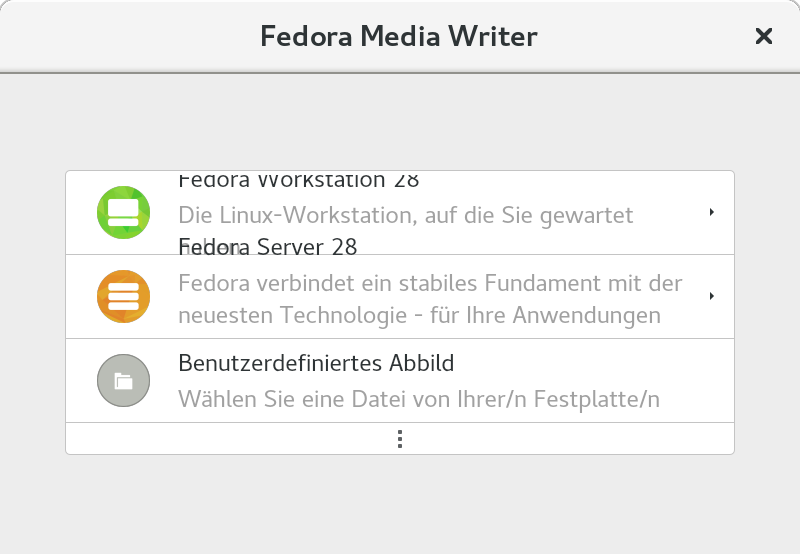
\includegraphics[scale=0.3]{Bilder/fmw1.png}
	\caption{FMW: Fedora Media Writer starten}
\end{figure}
\begin{figure}[H]
	\centering
	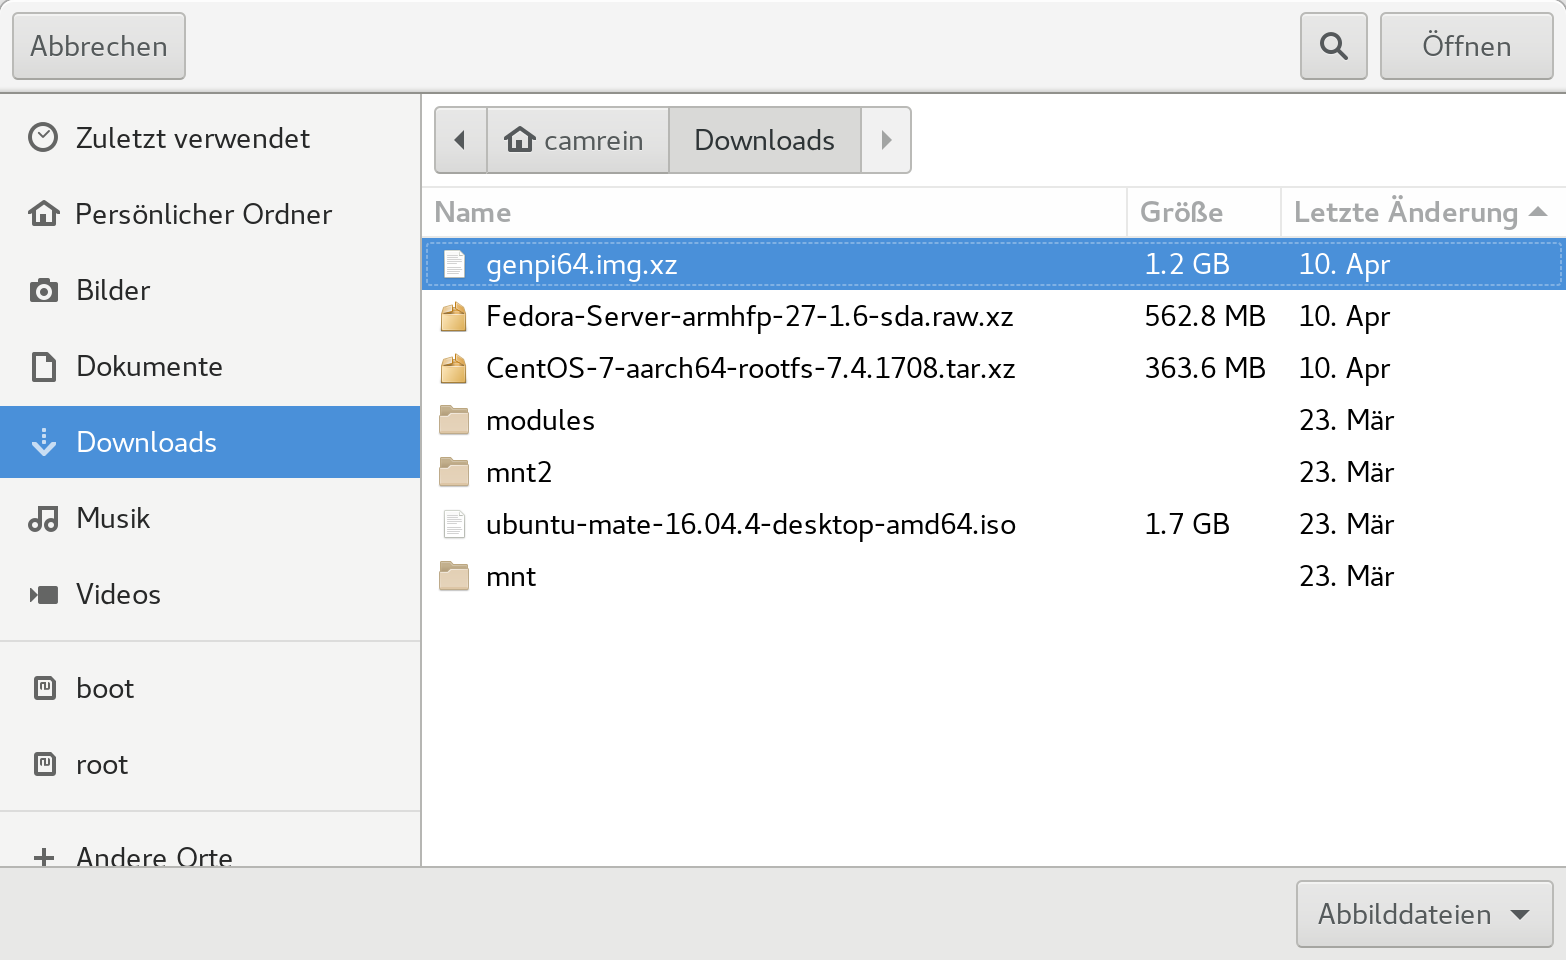
\includegraphics[scale=0.2]{Bilder/fmw2.png}
	\caption{FMW: Archiv auswählen}
\end{figure}
\begin{figure}[H]
	\centering
	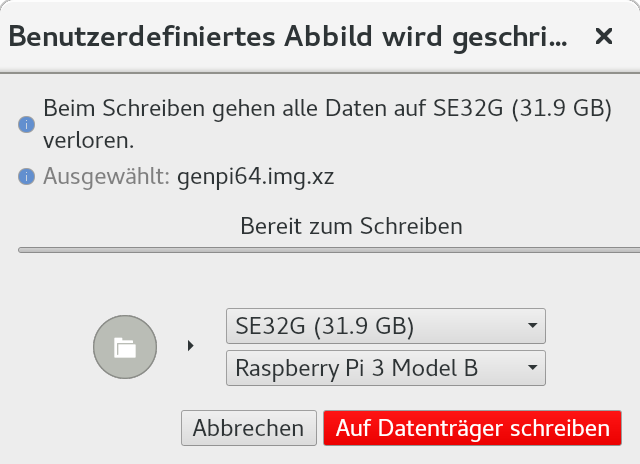
\includegraphics[scale=0.3]{Bilder/fmw3.png}
	\caption{FMW: Abbild schreiben}
\end{figure}
3. Durch das Schreiben des Archivs wurden zwei Partitionen (boot \& rootfs) auf der SD Karte erstellt. Diese werden wie folgt ausgelesen:
\begin{lstlisting}
[camrein@wifibridge ~]\$ lsblk
NAME MAJ:MIN RM SIZE RO TYPE MOUNTPOINT
sda 8:0 0 238.5G 0 disk 
-sda1 8:1 0 200M 0 part /boot/efi
-sda2 8:2 0 1G 0 part /boot
-sda3 8:3 0 237.3G 0 part 
--fedora-root 253:0 0 50G 0 lvm /
--fedora-swap 253:1 0 7.8G 0 lvm [SWAP]
--fedora-home 253:2 0 179.5G 0 lvm /home
mmcblk0 179:0 0 29.7G 0 disk}
-mmcblk0p1 179:1 0 43.1M 0 part /run/media/camrein/boot
-mmcblk0p2 179:2 0 29.7G 0 part /run/media/camrein/rootfs
[camrein@wifibridge ~]\$
\end{lstlisting}
4. Die Dateisystem-Partition muss mit der von CentOS überschrieben werden. Dazu wird die Partition auf dem Linux Client angehängt. Bei Schritt 5-7 wird überprüft, ob die Partition wirklich leer ist.
\begin{lstlisting}
[root@wifibridge Downloads]# mkdir mnt
[root@wifibridge Downloads]# mount /dev/mmcblk0p2 mnt
[root@wifibridge Downloads]# cd mnt
[root@wifibridge mnt]# rm -rf *
[root@wifibridge mnt]# ls -lrtha
drwxr-xr-x. 5 camrein camrein 20K 15. Mai 17:39 ..
drwxr-xr-x. 2 root root 4.0K 16. Mai 17:58 .
\end{lstlisting}

Die Dateisystem-Partition ist nun leer und kann mit der von CentOS überschrieben werden. \newline
5. Das Dateisystem aus dem offiziellen Centos Repository\footnote{\url{http://mirror.centos.org/altarch/7.4.1708/isos/aarch64/CentOS-7-aarch64-rootfs-7.4.1708.tar.xz}} beziehen. \newline
6. Die geleerte Partition wird nun mit dem Dateisystem von Centos7.4 überschrieben. Zugleich soll bei Schritt 2 überprüft werden, ob die Daten wirklich auf die Partition geschrieben wurden.
\begin{lstlisting}
[root@wifibridge mnt]# tar --numeric-owner -xpJf ../CentOS-7-aarch64-rootfs-7.4.1708.tar.xz
[root@wifibridge mnt]# ls -lrtha
insgesamt 84K
drwxr-xr-x. 2 root root 4.0K 23. Nov 2016 srv
drwxr-xr-x. 2 root root 4.0K 23. Nov 2016 opt
drwxr-xr-x. 2 root root 4.0K 23. Nov 2016 mnt
drwxr-xr-x. 2 root root 4.0K 23. Nov 2016 media
drwxr-xr-x. 2 root root 4.0K 23. Nov 2016 home
drwxr-xr-x. 2 root root 4.0K 12. Sep 2017 dev
drwxr-xr-x. 2 root root 4.0K 12. Sep 2017 proc
drwxr-xr-x. 2 root root 4.0K 12. Sep 2017 run
drwxr-xr-x. 2 root root 4.0K 12. Sep 2017 sys
lrwxrwxrwx. 1 root root 7 12. Sep 2017 bin -> usr/bin
lrwxrwxrwx. 1 root root 8 12. Sep 2017 sbin -> usr/sbin
lrwxrwxrwx. 1 root root 9 12. Sep 2017 lib64 -> usr/lib64
lrwxrwxrwx. 1 root root 7 12. Sep 2017 lib -> usr/lib
drwxr-xr-x. 13 root root 4.0K 12. Sep 2017 usr
drwxr-xr-x. 19 root root 4.0K 12. Sep 2017 var
dr-xr-xr-x. 17 root root 4.0K 12. Sep 2017 .
drwxr-xr-x. 82 root root 4.0K 12. Sep 2017 etc
dr-xr-xr-x. 3 root root 4.0K 12. Sep 2017 boot
drwxrwxrwt. 7 root root 4.0K 12. Sep 2017 tmp
dr-xr-x---. 2 root root 4.0K 12. Sep 2017 root
drwxr-xr-x. 5 camrein camrein 20K 15. Mai 17:39 ..
[root@wifibridge mnt]#
\end{lstlisting}

Die SD Karte kann nun mit den RPI's verwendet werden. Diese starten jeweils mit dem Hostnamen centos.


\subsection{RPI für den Netzwerkboot vorbereiten}
Für das Vorbereiten der Clients für den Netzwerkboot wurde der Guide NETWORK BOOT YOUR RASPBERRY PI von raspberrypi.org\footnote{\url{https://www.raspberrypi.org/documentation/hardware/raspberrypi/bootmodes/net\_tutorial.md}} verwendet. Die RPI's werden wie folgt vorbereitet:

1. Die config.txt Datei im /boot Verzeichnis benötigt einen OTP Eintrag, dieser sagt aus, dass das RPI ohne SD Karte nach einem Betriebssystem anfragen soll. 
\begin{lstlisting}
echo program_usb_boot_mode=1 | sudo tee -a /boot/config.txt
\end{lstlisting}
2. RPI neu starten. \newline
3. Prüfen, ob die Änderung aktiv ist.
\begin{lstlisting}
vcgencmd otp_dump | grep 17:
\end{lstlisting}
Erwartetes Ergebnis:
\begin{lstlisting}
17:3020000a
\end{lstlisting}
4. Den Eintrag in der /boot/config.txt wieder entfernen.\newline
\textbf{MAC-Adressen auslesen}\newline
Um Zeit zu sparen können alle MAC-Adressen der RPI's während der Vorbereitung der Clients auf den Netzwerkboot ausgelesen werden.\newline
5. nmap Scan auf die IP Range 192.168.1.0-255 von einem Linux Client aus durchführen.
\begin{lstlisting}
	  nmap -sP 192.168.1.0/24  
\end{lstlisting}
Erwartetes Ergebnis für ein RPI:
\begin{lstlisting}
	  Nmap scan report for centos.home (192.168.1.11)
	  Host is up (0.00055s latency).
	  MAC Address: B8:27:EB:32:39:A7 (Raspberry Pi Foundation)   
\end{lstlisting}

Die Vorbereitung der RPI(Compute Nodes) ist somit abgeschlossen und es kann mit der Installation des Management Node fortgefahren werden.

\subsection{Hostname und IP der MAC Adresse zuweisen}
über http://internetbox/ wird die IP Adresse sowie der Hostname der MAC Adresse der RPI's zugewiesen. Alle jemals angeschlossenen Geräte werden unter der Geräteliste aufgelistet. Dort können ebenfalls die Hostnamen den Geräten zugewiesen werden.

\begin{figure}[H]
	\centering
	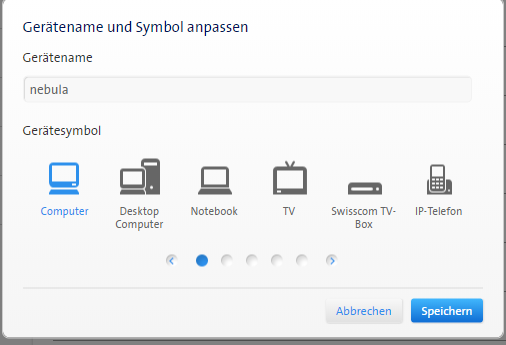
\includegraphics[scale=0.8]{Bilder/hostnamen_mac_edit.png}
	\caption{Hostnamen editieren}
\end{figure}
\begin{figure}[H]
	\centering
	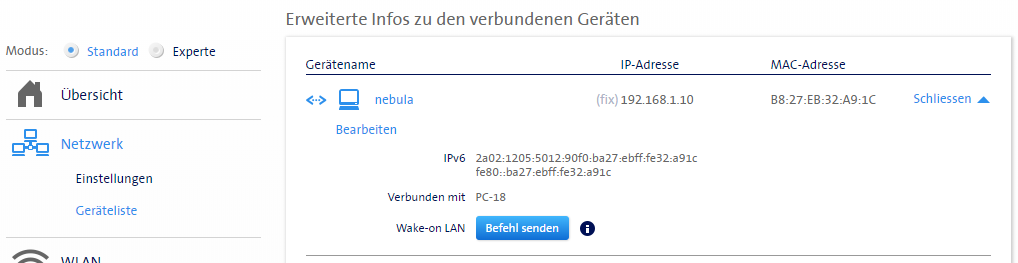
\includegraphics[scale=0.6]{Bilder/hostnamen_mac_overview.png}
	\caption{Übersicht der Hostnamen Zuweisung}
\end{figure}

Die fixe IP Adresse wird unter den Netzwerkeinstellungen des Routers direkt vorgenommen. Hierbei kann den bereits erkannten und definierten RPI's per Hostname eine IP zugewiesen werden.
\begin{figure}[H]
	\centering
	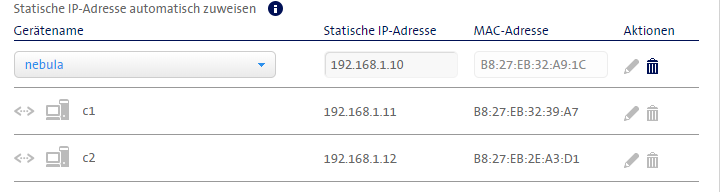
\includegraphics[scale=0.8]{Bilder/ip_mac_edit.png}
	\caption{Statische IP vergeben}
\end{figure}

\subsection{Netzwerkshare einrichten}
Der Netzwerkshare wird über das Synology NAS mit dem Network File System (NFS) Protkoll bereitgestellt. Der Share wird gemäss den aufgelisteten Schritten erstellt. \newline

1. Über den Browser auf das NAS via http://influbox/ verbinden. \newline
2. Anmeldedaten eingeben. \newline
3. Über die Systemsteuerung die Einstellungen für Dateidienste aufrufen. \newline
4. Unter dem Reiter SMB/AFP/NFS soll die Funktion \grqq NFS aktivieren\grqq aktiviert werden. \newline
5. Der NFS Dienst ist nun aktiviert und es kann unter \grqq Gemeinsam Ordner\grqq ein neues Verzeichnis angelegt werden. Dieses Verzeichnis wird der Mountpoint für die Nodes. Der Mountpoint wurde nebula genannt. \newline
6. Für den erstellten Ordner müssen nun noch die Berechtigungen für Zugriffe eingerichtet werden. Dazu bearbeitet man unter Einstellungen die Rechte auf das Verzeichnis. \newline
7. Damit nicht jeder das Verzeichnis mounten kann, wurde  auf 192.168.10/24  eingegrenzt. Dies kann über das GUI von Synology direkt eingerichtet werden.
\begin{figure}[H]
	\centering
	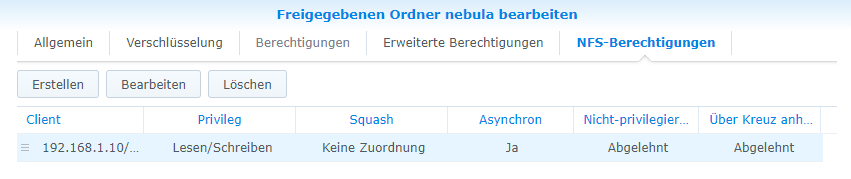
\includegraphics[scale=0.8]{Bilder/nfs_net.png}
	\caption{NFS: Erlaubte Clients}
\end{figure}
8. Der Netzwerkshare kann von nun an auf dem Management Node und den Computes eingebunden werden.
% !TEX root = ../Diplombericht.tex

\section{Installation Management Node}
Die Serverinstallation des Management Nodes wird nach dem offiziellen OpenHPC Guide mit einigen Abweichungen durchgeführt. Die Installation basiert auf der Anleitung CentOS 7.4 aarch64 Install guide with Warewulf + Slurm \footnote{\url{http://openhpc.community/downloads/}}. Die Installation wird hauptsächlich mit dem ROOT-Benutzer durchgeführt, falls nichts anderes erwähnt wird.

\subsection{Variablen Definition}
Durch die Installation hinweg werden die folgenden Variablen verwendet:

\begin{longtable}{| p{0.5cm} | p{3cm} | p{8.5cm} | p{4cm} |} 
\hline
\rowcolor{heading} \textbf{Nr.} & \textbf{Variable} & \textbf{Beschreibung} &\textbf{Werte} \\\hline
1 & sms\_name & Hostname des Managementhosts & nebula \\\hline
2 & sms\_ip & IP Adresse des Managementhosts & 192.168.1.10 \\\hline
3 & sms\_eth\_internal & Ethernet Interface & eth0 \\\hline
4 & ntp\_server[0] \newline ntp\_server[1] \newline ntp\_server[2] \newline ntp\_server[3] & Zeitserver (Array) & server 0.ch.pool.ntp.org \newline server 1.ch.pool.ntp.org \newline server 2.ch.pool.ntp.org \newline server 3.ch.pool.ntp.org  \\\hline
5 & num\_computes & Anzahl Compute Nodes & 45 \\\hline
6 &  c\_ip[0] \newline  c\_ip[1] \newline c\_ip[2] \newline c\_ip[3] \newline c\_ip[4] \newline c\_ip[5] \newline c\_ip[6] \newline c\_ip[7] \newline c\_ip[8] \newline c\_ip[9] \newline c\_ip[10] \newline c\_ip[11] \newline c\_ip[12] \newline c\_ip[13] \newline c\_ip[14] \newline c\_ip[15] \newline c\_ip[16] \newline c\_ip[17] \newline c\_ip[18] & IP Adressen der Compute Nodes (Array) & 192.168.1.11 \newline 192.168.1.12 \newline 192.168.1.13 \newline 192.168.1.14 \newline 192.168.1.15 \newline 192.168.1.16 \newline 192.168.1.17 \newline 192.168.1.18 \newline 192.168.1.19 \newline 192.168.1.20 \newline 192.168.1.21 \newline 192.168.1.22 \newline 192.168.1.23 \newline 192.168.1.24 \newline 192.168.1.25 \newline 192.168.1.26 \newline 192.168.1.27 \newline 192.168.1.28 \newline 192.168.1.29 \\\hline 
\rowcolor{heading} \textbf{Nr.} & \textbf{Variable} & \textbf{Beschreibung} &\textbf{Werte} \\\hline
6 & c\_ip[19] \newline c\_ip[20] \newline c\_ip[21] \newline c\_ip[22] \newline c\_ip[23] \newline c\_ip[24]  \newline c\_ip[25] \newline c\_ip[26] \newline c\_ip[27] \newline c\_ip[28] \newline c\_ip[29]  \newline c\_ip[30] \newline c\_ip[31] \newline c\_ip[32] \newline c\_ip[33] \newline c\_ip[34] \newline c\_ip[35] \newline c\_ip[36] \newline c\_ip[37] \newline c\_ip[38] \newline c\_ip[39] \newline c\_ip[40] \newline c\_ip[41] \newline c\_ip[42] \newline c\_ip[43] \newline c\_ip[44] & IP Adressen der Compute Nodes (Array) &  192.168.1.30 \newline 192.168.1.31 \newline 192.168.1.32 \newline  192.168.1.33 \newline 192.168.1.34 \newline 192.168.1.35 \newline 192.168.1.36 \newline 192.168.1.37 \newline 192.168.1.38 \newline 192.168.1.39 \newline 192.168.1.40 \newline 192.168.1.41 \newline 192.168.1.42 \newline 192.168.1.43 \newline 192.168.1.44 \newline 192.168.1.45 \newline 192.168.1.46 \newline 192.168.1.47 \newline 192.168.1.48 \newline 192.168.1.49 \newline 192.168.1.50 \newline 192.168.1.51 \newline 192.168.1.52 \newline 192.168.1.53 \newline 192.168.1.54 \newline 192.168.1.55 \\\hline 
7 &  c\_name[0] \newline  c\_name[1] \newline c\_name[2] \newline c\_name[3] \newline c\_name[4] \newline c\_name[5] \newline c\_name[6] \newline c\_name[7] \newline c\_name[8] \newline c\_name[9] \newline c\_name[10] \newline c\_name[11] \newline c\_name[12]  & Hostnamen der Compute Nodes (Array) & c1 \newline c2 \newline c3 \newline c4 \newline c5 \newline c6 \newline c7 \newline c8 \newline c9 \newline c10 \newline c11 \newline c12 \newline c13 \\\hline 
\rowcolor{heading} \textbf{Nr.} & \textbf{Variable} & \textbf{Beschreibung} &\textbf{Werte} \\\hline
7 & c\_name[13] \newline c\_name[14] \newline c\_name[15] \newline c\_name[16] \newline c\_name[17] \newline c\_name[18] \newline c\_name[19] \newline c\_name[20] \newline c\_name[21] \newline c\_name[22] \newline c\_name[23] \newline c\_name[24] \newline c\_name[25] \newline c\_name[26] \newline c\_name[27] c\_name[28] \newline  c\_name[29] \newline c\_name[30] \newline c\_name[31] \newline c\_name[32] \newline c\_name[33] \newline c\_name[34] \newline c\_name[35] \newline c\_name[36] \newline c\_name[37] \newline c\_name[38] \newline c\_name[39] \newline c\_name[40] \newline c\_name[41] \newline c\_name[42] \newline c\_name[43] \newline c\_name[44] & Hostnamen der Compute Nodes (Array) &   c14 \newline c15 \newline c16 \newline c17 \newline c18 \newline c19 \newline c20 \newline c21 \newline c22 \newline c23 \newline c24 \newline c25 \newline c26 \newline c27 \newline c28 \newline c29 \newline c30 \newline c31 \newline c32 \newline c33 \newline c34 \newline c35 \newline c36 \newline c37 \newline c38 \newline c39 \newline c40 \newline c41 \newline c42 \newline c43 \newline c44 \newline c45\\\hline 
8 &  c\_mac[0] \newline  c\_mac[1] \newline c\_mac[2] \newline c\_mac[3] \newline c\_mac[4] \newline c\_mac[5] \newline c\_mac[6]   & MAC Adressen der Compute Nodes (Array) & B8:27:EB:32:39:A7 \newline B8:27:EB:2E:A3:D1 \newline B8:27:EB:50:45:3F \newline B8:27:EB:0D:E6:25 \newline B8:27:EB:3E:96:B5 \newline B8:27:EB:EE:77:DA \newline B8:27:EB:21:63:E6 \\\hline 
\rowcolor{heading} \textbf{Nr.} & \textbf{Variable} & \textbf{Beschreibung} &\textbf{Werte} \\\hline
8 & c\_mac[7] \newline c\_mac[8] \newline c\_mac[9] \newline  c\_mac[10] \newline c\_mac[11] \newline c\_mac[12] \newline c\_mac[13] \newline c\_mac[14] \newline c\_mac[15] \newline c\_mac[16] \newline c\_mac[17] \newline c\_mac[18] \newline c\_mac[19] \newline c\_mac[20] \newline c\_mac[21] \newline c\_mac[22] \newline c\_mac[23] \newline c\_mac[24] \newline c\_mac[25] \newline c\_mac[26] \newline c\_mac[27] \newline c\_mac[28] \newline c\_mac[29] \newline c\_mac[30] \newline c\_mac[31] \newline c\_mac[32] \newline c\_mac[33] \newline c\_mac[34] \newline c\_mac[35] \newline c\_mac[36] \newline c\_mac[37] \newline c\_mac[38] \newline c\_mac[39] \newline c\_mac[40] \newline c\_mac[41] \newline c\_mac[42] \newline c\_mac[43] \newline c\_mac[44] & MAC Adressen der Compute Nodes (Array) & B8:27:EB:2E:2E:CC \newline B8:27:EB:17:32:96 \newline B8:27:EB:B2:1C:A9 \newline B8:27:EB:AF:63:1F \newline B8:27:EB:43:00:2C \newline B8:27:EB:13:7B:18 \newline B8:27:EB:43:CD:29 \newline B8:27:EB:FF:C7:56 \newline B8:27:EB:CE:98:66 \newline B8:27:EB:5D:63:34 \newline B8:27:EB:91:3E:0F \newline B8:27:EB:F4:65:EC \newline B8:27:EB:3E:AB:DC \newline B8:27:EB:66:60:F6 \newline B8:27:EB:37:3F:74 \newline B8:27:EB:18:5E:F0 \newline B8:27:EB:B0:23:B8 \newline B8:27:EB:BE:C4:94 \newline B8:27:EB:FB:FF:57 \newline B8:27:EB:4E:EC:CE \newline 	B8:27:EB:43:1C:35 \newline B8:27:EB:DC:74:5F \newline B8:27:EB:D1:DE:2F \newline B8:27:EB:5E:90:34 \newline B8:27:EB:DE:80:24 \newline B8:27:EB:A4:79:6F \newline B8:27:EB:0A:4D:C7 \newline B8:27:EB:5C:53:5F \newline B8:27:EB:F7:AF:C2 \newline B8:27:EB:CE:BA:ED \newline B8:27:EB:59:38:3C \newline B8:27:EB:99:BB:8E \newline B8:27:EB:8F:7A:0D \newline B8:27:EB:DE:C9:69 \newline B8:27:EB:7E:6F:48 \newline B8:27:EB:5D:DD:FE
\newline B8:27:EB:A6:6D:4D \newline B8:27:EB:0C:63:10\\\hline 
\caption{Variablen Definition}
\end{longtable}

\subsection{Basiskonfiguration}
Dem Management Node muss ein eindeutiger Hostname zugewiesen werden. Hierbei werden die untenstehenden Kommandos abgesetzt:

\begin{lstlisting}
echo ${sms_ip} ${sms_name} >> /etc/hosts
hostnamectl set-hostname ${sms_name}
\end{lstlisting}

Für die folgenden Arbeiten müssen die Firewall und SELinux deaktiviert werden. DHCP wird aufgrund der Verwendung von dnsmasq deaktivert.

\begin{lstlisting}
systemctl disable firewalld
systemctl stop firewalld
systemctl disable dhcpd
systemctl stop dhcpd
echo 0 > /selinux/enforce
\end{lstlisting}

\subsection{OpenHPC Komponenten installieren}
Es wird das OpenHPC Repository für die Installation der OpenHPC Komponenten benötigt. Dieses muss installiert werden:

\begin{lstlisting}
yum install http://build.openhpc.community/OpenHPC:/1.3/CentOS_7/aarch64/ohpc-release-1.3-1.el7.aarch64.rpm
\end{lstlisting}

Von nun an können die benötigten Pakete über den Red Hat Package Manager (RPM-Paketmanager) installiert werden.

Durch das neu angehängte Repository können nun die folgenden Pakete installiert werden:

\begin{lstlisting}
yum -y install ohpc-base
yum -y install ohpc-warewulf
\end{lstlisting}

Weiterhin spielt die Zeit eine wichtige Rolle zwischen der Kommunikation des Managementhosts und der Compute Nodes. Dazu müssen die bereits vorhandenen Einträge der Zeitserver in der ntp.conf entfernt werden.


\begin{lstlisting}
systemctl disable chronyd.service
systemctl stop chronyd.service
systemctl enable ntpd.service
sed -i '/^server/ d' /etc/ntp.conf
echo "server ${ntp_server[0]}" >> /etc/ntp.conf
echo "server ${ntp_server[1]}" >> /etc/ntp.conf
echo "server ${ntp_server[2]}" >> /etc/ntp.conf
echo "server ${ntp_server[3]}" >> /etc/ntp.conf
systemctl restart ntpd
\end{lstlisting}

Nun wird der Slurmcontroller installiert. Dieser dient dazu, die Jobs auf die Compute Nodes zu verteilen. Dieser steuert die Jobverwaltung und muss installiert und eingerichtet werden. Hierbei wird die Konfiguration für 45 Compute Nodes vorgenommen.

\begin{lstlisting}
yum -y install ohpc-slurm-server
perl -pi -e "s/ControlMachine=\S+/ControlMachine=${sms_name}/" /etc/slurm/slurm.conf
sed -i '/^NodeName/ d' /etc/slurm/slurm.conf
sed -i '/^Partition/ d' /etc/slurm/slurm.conf
echo "NodeName=c[1-45] CoresPerSocket=1 ThreadsPerCore=1 SocketsPerBoard=4 State=UNKNOWN" >> /etc/slurm/slurm.conf
echo "PartitionName=normal Nodes=c[1-45] Default=YES MaxTime=INFINITE State=UP" >> /etc/slurm/slurm.conf
\end{lstlisting}

\subsection{Netzwerkboot einrichten}
Das Dateisystem und die Boot-Partition werden in zwei verschiedenen Verzeichnissen erstellt und abgelegt.

Definieren des Dateisystem-Verzeichnisses und das Centos7.4 Basis-Dateisystem erstellen.
\begin{lstlisting}
export CHROOT=/opt/ohpc/admin/images/centos7.4
wwmkchroot centos-7 $CHROOT
\end{lstlisting}

Anstelle von DHCPD muss der networking Service verwendet werden. Deshalb wird dieser aktiviert und gestartet.
\begin{lstlisting}
systemctl enable networking
systemctl start networking
\end{lstlisting}

Nun wird das Paket dnsmaq installiert. Dadurch wird die Verteilung des Betriebssystems an eine gewisse IP Range und an ein Subnetz gewährleistet. Geräte ausserhalb der Range und des Subnetzes sollen das Betriebssystem nicht erhalten dürfen.

\begin{lstlisting}
yum -y install dnsmasq
\end{lstlisting}

Nach der Installation kann die Konfiguration von dnsmasq vorgenommen werden. Dazu werden die Datei /etc/dnsmasq.conf angepasst und die Datei /etc/dnsmasq.d/host.allow erstellt.

In der dnsmasq.conf Datei wird das Konfigurationsverzeichnis für die erlaubten Hosts erstellt, zudem wird eine IP Range angegeben, alle Geräte innerhalb dieser Range dürfen den Kernel des Betriebssystems aus dem Verzeichnis /tftboot erhalten.  
\begin{lstlisting}
[root@nebula etc]# cat /etc/dnsmasq.conf
conf-dir=/etc/dnsmasq.d
port=0
dhcp-range=192.168.1.10,192.168.1.50,12h
log-dhcp
enable-tftp
tftp-root=/tftpboot
pxe-service=0,"Raspberry Pi Boot"
\end{lstlisting}

Falls sich andere Geräte in dieser IP Range befinden, wird dies durch die /etc/dnsmasq.d/host.allow Datei abgefangen. Dort sind alle Compute Nodes mit MAC Adresse, Hostnamen und IP Adresse hinterlegt.

Die host.allow Datei kann in einer for Schlaufe mit den definierten Variablen einfach abgefüllt werden.

\begin{lstlisting}
for ((i=0; i<45; i++)); do echo "dhcp-host=${c_mac[$i]};${c_name[$i]};${c_ip[$i]}" >> /etc/dnsmasq.d/host.allow; done
\end{lstlisting}

Das Ergebnis muss wie folgt aussehen:
\begin{lstlisting}
[root@nebula etc]# cat /etc/dnsmasq.d/host.allow
dhcp-host=B8:27:EB:32:39:A7,c1,192.168.1.11
dhcp-host=B8:27:EB:2E:A3:D1,c2,192.168.1.12
dhcp-host=B8:27:EB:50:45:3F,c3,192.168.1.13
dhcp-host=B8:27:EB:0D:E6:25,c4,192.168.1.14
dhcp-host=B8:27:EB:3E:96:B5,c5,192.168.1.15
dhcp-host=B8:27:EB:EE:77:DA,c6,192.168.1.16
dhcp-host=B8:27:EB:21:63:E6,c7,192.168.1.17
dhcp-host=B8:27:EB:2E:2E:CC,c8,192.168.1.18
dhcp-host=B8:27:EB:17:32:96,c9,192.168.1.19
dhcp-host=B8:27:EB:B2:1C:A9,c10,192.168.1.20
dhcp-host=B8:27:EB:AF:63:1F,c11,192.168.1.21
dhcp-host=B8:27:EB:43:00:2C,c12,192.168.1.22
dhcp-host=B8:27:EB:13:7B:18,c13,192.168.1.23
dhcp-host=B8:27:EB:43:CD:29,c14,192.168.1.24
dhcp-host=B8:27:EB:FF:C7:56,c15,192.168.1.25
dhcp-host=B8:27:EB:CE:98:66,c16,192.168.1.26
dhcp-host=B8:27:EB:5D:63:34,c17,192.168.1.27
dhcp-host=B8:27:EB:91:3E:0F,c18,192.168.1.28
dhcp-host=B8:27:EB:F4:65:EC,c19,192.168.1.29
dhcp-host=B8:27:EB:3E:AB:DC,c20,192.168.1.30
dhcp-host=B8:27:EB:66:60:F6,c21,192.168.1.31
dhcp-host=B8:27:EB:37:3F:74,c22,192.168.1.32
dhcp-host=B8:27:EB:18:5E:F0,c23,192.168.1.33
dhcp-host=B8:27:EB:B0:23:B8,c24,192.168.1.34
dhcp-host=B8:27:EB:BE:C4:94,c25,192.168.1.35
dhcp-host=B8:27:EB:FB:FF:57,c26,192.168.1.36
dhcp-host=B8:27:EB:4E:EC:CE,c27,192.168.1.37
dhcp-host=B8:27:EB:43:1C:35,c28,192.168.1.38
dhcp-host=B8:27:EB:DC:74:5F,c29,192.168.1.39
dhcp-host=B8:27:EB:D1:DE:2F,c30,192.168.1.40
dhcp-host=B8:27:EB:5E:90:34,c31,192.168.1.41
dhcp-host=B8:27:EB:DE:80:24,c32,192.168.1.42
dhcp-host=B8:27:EB:A4:79:6F,c33,192.168.1.43
dhcp-host=B8:27:EB:0A:4D:C7,c34,192.168.1.44
dhcp-host=B8:27:EB:5C:53:5F,c35,192.168.1.45
dhcp-host=B8:27:EB:F7:AF:C2,c36,192.168.1.46
dhcp-host=B8:27:EB:CE:BA:ED,c37,192.168.1.47
dhcp-host=B8:27:EB:59:38:3C,c38,192.168.1.48
dhcp-host=B8:27:EB:99:BB:8E,c39,192.168.1.49
dhcp-host=B8:27:EB:8F:7A:0D,c40,192.168.1.50
dhcp-host=B8:27:EB:DE:C9:69,c41,192.168.1.51
dhcp-host=B8:27:EB:7E:6F:48,c42,192.168.1.52
dhcp-host=B8:27:EB:5D:DD:FE,c43,192.168.1.53
dhcp-host=B8:27:EB:A6:6D:4D,c44,192.168.1.54
dhcp-host=B8:27:EB:0C:63:10,c45,192.168.1.55
\end{lstlisting}

Boot-Verzeichnis erstellen. Aus diesem Verzeichnis wird der Kernel den Compute Nodes angeboten und übermittelt. Dabei wird das /boot Verzeichnis des Management Nodes in dieses Verzeichnis kopiert, da es sich um das selbe Betriebssystem handelt.

\begin{lstlisting}
[root@nebula /]# mkdir /tftpboot
[root@nebula /]# chmod 777 /tftpboot
[root@nebula /]# cp -r /boot /tftboot
\end{lstlisting}

Dabei muss darauf geachtet werden, dass die cmdline.txt Datei im /tftboot Verzeichnis folgenden Eintrag erhält. Dieser sagt aus, dass der Compute Node sein /root Verzeichnis vom Management Node unter dem Pfad /opt/ohpc/admin/images/centos7.4 beziehen soll.

\begin{lstlisting}
[root@nebula etc]# cat /tftpboot/cmdline.txt
dwc_otg.lpm_enable=0 root=/dev/nfs nfsroot=192.168.1.10:/opt/ohpc/admin/images/centos7.4,vers=3 rw ip=dhcp rootwait elevator=deadline
\end{lstlisting}

Zudem wird die config.txt angepasst. Hierbei wird die Taktrate der CPU auf 1400 MHz hochgetaktet. Dadurch steigt die Mining Performance von einer Hashrate 1.6 H/s auf 1.9 H/s.

\begin{lstlisting}
[root@nebula /]# echo "arm_freq=1400" > /tftpboot/config.txt
\end{lstlisting}


Den dnsmaq Service aktivieren und starten.
\begin{lstlisting}
[root@nebula /]# systemctl enable dnsmasq.service
[root@nebula /]# systemctl restart dnsmasq.service
\end{lstlisting}

OpenHPC Pakete für die Compute Nodes installieren.
\begin{lstlisting}
[root@nebula /]# yum -y --installroot=$CHROOT install ohpc-base-compute
\end{lstlisting}

Damit die Compute Nodes über den Hostnamen angesprochen werden können, wird eine Domain Name System (DNS) Konfiguration benötigt. Die Auflösung findet über folgende Einstellung statt. Dabei wird vom Management Node die resolv.conf Datei übernommen und auf das Dateisystem der Compute Nodes kopiert:
\begin{lstlisting}
[root@nebula /]# cp -p /etc/resolv.conf $CHROOT/etc/resolv.conf
\end{lstlisting}

Die zusätzlichen Pakete werden für die Kommunikation mit dem Slurmcontroller und der Zeitsynchronisierung benötigt.

\begin{lstlisting}
[root@nebula /]# yum -y --installroot=$CHROOT install ohpc-slurm-client
[root@nebula /]# yum -y --installroot=$CHROOT install ntp
\end{lstlisting}

Beim Booten der Compute Nodes muss das Dateisystem gemountet werden. Dafür werden fstab Einträge erstellt. Ausserdem wird auf der letzten Zeile der gemeinsame Netzwerkshare mit NFS angehängt.

\begin{lstlisting}
[root@nebula /]# echo "${sms_ip}:/home /home nfs nfsvers=3,nodev,nosuid,noatime 0 0" >> $CHROOT/etc/fstab
[root@nebula /]# echo "${sms_ip}:/opt/ohpc/pub /opt/ohpc/pub nfs nfsvers=3,nodev,noatime 0 0" >> $CHROOT/etc/fstab
[root@nebula /]# echo "192.168.1.129:/volume1/nebula /media/nebula_data nfs" >> $CHROOT/etc/fstab
\end{lstlisting}

Zudem müssen gewisse Verzeichnisse vom Management Node aus exportiert werden.

\begin{lstlisting}
[root@nebula /]# echo "/home *(rw,no_subtree_check,fsid=10,no_root_squash)" >> /etc/exports
[root@nebula /]# echo "echo "/opt/ohpc/pub *(ro,no_subtree_check,fsid=11)" >> /etc/exports
[root@nebula /]# echo "/opt/ohpc/admin/images/centos7.4 *(rw,sync,no_subtree_check,no_root_squash)" /etc/exports
[root@nebula /]# exportfs -a
[root@nebula /]# systemctl restart nfs-server
[root@nebula /]# systemctl enable nfs-server
\end{lstlisting}

Damit die Zeitsynchronisierung über den Management Node läuft, wird folgendes umgesetzt:

\begin{lstlisting}
[root@nebula /]# chroot $CHROOT systemctl enable ntpd
[root@nebula /]# echo "server ${sms_ip}" >> $CHROOT/etc/ntp.conf
\end{lstlisting}

Die Compute Nodes können nun mit Strom versorgt werden. Dabei wird auf dem Management Node auf die /var/log/messages Logdatei geachtet. Dort sind alle Einträge des Netzwerkboots zusammengeschlossen. Dabei müssen folgende Einträge erscheinen:

\begin{lstlisting}
May 17 20:31:34 nebula dnsmasq-dhcp[382]: 653460281 next server: 192.168.1.10
May 17 20:31:34 nebula dnsmasq-dhcp[382]: 653460281 sent size:  1 option: 53 message-type  2
May 17 20:31:34 nebula dnsmasq-dhcp[382]: 653460281 sent size:  4 option: 54 server-identifier  192.168.1.10
May 17 20:31:34 nebula dnsmasq-dhcp[382]: 653460281 sent size:  4 option: 51 lease-time  12h
May 17 20:31:34 nebula dnsmasq-dhcp[382]: 653460281 sent size:  4 option: 58 T1  6h
May 17 20:31:34 nebula dnsmasq-dhcp[382]: 653460281 sent size:  4 option: 59 T2  10h30m
May 17 20:31:34 nebula dnsmasq-dhcp[382]: 653460281 sent size:  4 option:  1 netmask  255.255.255.0
May 17 20:31:34 nebula dnsmasq-dhcp[382]: 653460281 sent size:  4 option: 28 broadcast  192.168.1.255
May 17 20:31:34 nebula dnsmasq-dhcp[382]: 653460281 sent size:  9 option: 60 vendor-class  50:58:45:43:6c:69:65:6e:74
May 17 20:31:34 nebula dnsmasq-dhcp[382]: 653460281 sent size: 17 option: 97 client-machine-id  00:44:44:44:44:44:44:44:44:44:44:44:44:44...
May 17 20:31:34 nebula dnsmasq-dhcp[382]: 653460281 sent size: 32 option: 43 vendor-encap  06:01:03:0a:04:00:50:58:45:09:14:00:00:11...
May 17 20:31:34 nebula dnsmasq-dhcp[382]: 653460281 available DHCP range: 192.168.1.10 -- 192.168.1.50
May 17 20:31:34 nebula dnsmasq-dhcp[382]: 653460281 vendor class: PXEClient:Arch:00000:UNDI:002001
..
..
..
May 17 20:31:35 nebula dnsmasq-tftp[382]: sent /tftpboot/bootcode.bin to 192.168.1.46
May 17 20:31:35 nebula dnsmasq-tftp[382]: file /tftpboot/autoboot.txt not found
May 17 20:31:35 nebula dnsmasq-tftp[382]: sent /tftpboot/config.txt to 192.168.1.38
May 17 20:31:35 nebula dnsmasq-tftp[382]: file /tftpboot/recovery.elf not found
May 17 20:31:35 nebula dnsmasq-tftp[382]: file /tftpboot/beb21ca9/start.elf not found
May 17 20:31:35 nebula dnsmasq-tftp[382]: file /tftpboot/75a66d4d/start.elf not found
May 17 20:31:35 nebula dnsmasq-tftp[382]: file /tftpboot/d0185ef0/start.elf not found
May 17 20:31:35 nebula dnsmasq-tftp[382]: file /tftpboot/10dec969/start.elf not found
May 17 20:31:35 nebula dnsmasq-tftp[382]: file /tftpboot/d4373f74/start.elf not found
May 17 20:31:35 nebula dnsmasq-tftp[382]: file /tftpboot/0643cd29/start.elf not found
May 17 20:31:35 nebula dnsmasq-tftp[382]: file /tftpboot/bootsig.bin not found
May 17 20:31:35 nebula dnsmasq-tftp[382]: sent /tftpboot/bootcode.bin to 192.168.1.40
May 17 20:31:35 nebula dnsmasq-tftp[382]: file /tftpboot/bootsig.bin not found
May 17 20:31:35 nebula dnsmasq-tftp[382]: sent /tftpboot/bootcode.bin to 192.168.1.16
May 17 20:31:35 nebula dnsmasq-tftp[382]: file /tftpboot/bootsig.bin not found
May 17 20:31:35 nebula dnsmasq-tftp[382]: sent /tftpboot/bootcode.bin to 192.168.1.27
..
..
..
May 17 20:32:56 nebula dnsmasq-dhcp[382]: 925035958 next server: 192.168.1.10
May 17 20:32:56 nebula dnsmasq-dhcp[382]: 925035958 sent size:  1 option: 53 message-type  2
May 17 20:32:56 nebula dnsmasq-dhcp[382]: 925035958 sent size:  4 option: 54 server-identifier  192.168.1.10
May 17 20:32:56 nebula dnsmasq-dhcp[382]: 925035958 sent size:  4 option: 51 lease-time  12h
May 17 20:32:56 nebula dnsmasq-dhcp[382]: 925035958 sent size:  4 option: 58 T1  6h
May 17 20:32:56 nebula dnsmasq-dhcp[382]: 925035958 sent size:  4 option: 59 T2  10h30m
May 17 20:32:56 nebula dnsmasq-dhcp[382]: 925035958 sent size:  4 option:  1 netmask  255.255.255.0
May 17 20:32:56 nebula dnsmasq-dhcp[382]: 925035958 sent size:  4 option: 28 broadcast  192.168.1.255
May 17 20:32:56 nebula dnsmasq-dhcp[382]: 925035958 sent size:  4 option:  3 router  192.168.1.10
May 17 20:32:56 nebula dnsmasq-dhcp[382]: 925035958 sent size:  3 option: 12 hostname  c12
May 17 20:32:56 nebula dnsmasq-dhcp[382]: 925035958 available DHCP range: 192.168.1.10 -- 192.168.1.50
May 17 20:32:56 nebula rpc.mountd[495]: authenticated mount request from 192.168.1.22:999 for /opt/ohpc/admin/images/centos7.4 (/opt/ohpc/admin/images/centos7.4)
\end{lstlisting}

Durch die letzte Zeile (authenticated mount request from 192.168.1.22) ist ersichtlich, dass der Compute Node c12 gestartet wurde und nach dem Betriebssystem angefragt hat und dieses mounten will.
\newpage

\subsection{Netzwerkshare einbinden}

Der Netzwerkshare wird über NFS auf dem Management Node eingebunden. Dies wird mit einem Eintrag in /etc/fstab erledigt. Dadurch ist bei einem Neustart der Netzwerkshare automatisch wieder verbunden.
\begin{lstlisting}
[root@nebula /]# echo "192.168.1.129:/volume1/nebula /media/nebula_data nfs" >> /etc/fstab
\end{lstlisting}

\subsection{Registration Compute Nodes}

Die Basisinstallation ist soweit abgeschlossen. Nun werden die Compute Nodes registriert. Ab diesem Zeitpunkt kennt der Management Node jeden Compute Node. Die Compute Nodes werden wie folgt in den Datastore aufgenommen:

\begin{lstlisting}
[root@nebula /]# echo "GATEWAYDEV=${eth_internal}" > /tmp/network.$$
[root@nebula /]# wwsh -y file import /tmp/network.$$ --name network
[root@nebula /]# wwsh -y file set network --path /etc/sysconfig/network --mode=0644 --uid=0
[root@nebula /]# for ((i=0; i<$num_computes; i++)) ; do
[root@nebula /]# wwsh -y node new ${c_name[i]} --ipaddr=${c_ip[i]} --hwaddr=${c_mac[i]} -D ${eth_internal}
done
\end{lstlisting}
\newpage
\subsection{Monitoring installieren}

Das Nagios Monitoring wird wie folgt installiert. Dabei werden alle Grundüberwachungen installiert und können Out of the Box verwendet werden:

\begin{lstlisting}
[root@nebula /]# yum -y install ohpc-nagios
[root@nebula /]# yum -y --installroot=$CHROOT install nagios-plugins-all-ohpc nrpe-ohpc
[root@nebula /]# chroot $CHROOT systemctl enable nrpe
[root@nebula /]# perl -pi -e "s/^allowed_hosts=/# allowed_hosts=/" $CHROOT/etc/nagios/nrpe.cfg
[root@nebula /]# echo "nrpe 5666/tcp # NRPE" >> $CHROOT/etc/services
[root@nebula /]# echo "nrpe : ${sms_ip} : ALLOW" >> $CHROOT/etc/hosts.allow
[root@nebula /]# echo "nrpe : ALL : DENY" >> $CHROOT/etc/hosts.allow
[root@nebula /]# chroot $CHROOT /usr/sbin/useradd -c "NRPE user for the NRPE service" -d /var/run/nrpe -r -g nrpe -s /sbin/nologin nrpe
[root@nebula /]# chroot $CHROOT /usr/sbin/groupadd -r nrpe
[root@nebula /]# mv /etc/nagios/conf.d/services.cfg.example /etc/nagios/conf.d/services.cfg
[root@nebula /]# mv /etc/nagios/conf.d/hosts.cfg.example /etc/nagios/conf.d/hosts.cfg
[root@nebula /]# for ((i=0; i<$num_computes; i++)) ; do
perl -pi -e "s/HOSTNAME$(($i+1))/${c_name[$i]}/ || s/HOST$(($i+1))_IP/${c_ip[$i]}/" \
[root@nebula /]# /etc/nagios/conf.d/hosts.cfg
done
[root@nebula /]# perl -pi -e "s/ \/bin\/mail/ \/usr\/bin\/mailx/g" /etc/nagios/objects/commands.cfg
[root@nebula /]# perl -pi -e "s/nagios\@localhost/root\@${sms_name}/" /etc/nagios/objects/contacts.cfg
[root@nebula /]# echo command[check_ssh]=/usr/lib64/nagios/plugins/check_ssh localhost >> $CHROOT/etc/nagios/nrpe.cfg
[root@nebula /]# htpasswd -bc /etc/nagios/passwd nagiosadmin ${Eigenes_Passwort}
[root@nebula /]# chkconfig nagios on
[root@nebula /]# systemctl start nagios
[root@nebula /]# chmod u+s `which ping
\end{lstlisting}

Nagios kann nun eingesetzt werden und ist über http://nebula/nagios erreichbar.

Das Performance Monitoring wird mit Ganglia realisiert, welches sich wie folgt installieren lässt:

\begin{lstlisting}
[root@nebula /]# yum -y install ohpc-ganglia
[root@nebula /]# yum -y --installroot=$CHROOT install ganglia-gmond-ohpc
[root@nebula /]# cp /opt/ohpc/pub/examples/ganglia/gmond.conf /etc/ganglia/gmond.conf
[root@nebula /]# perl -pi -e "s/<sms>/${sms_name}/" /etc/ganglia/gmond.conf
[root@nebula /]# cp /etc/ganglia/gmond.conf $CHROOT/etc/ganglia/gmond.conf
echo "gridname MySite" >> /etc/ganglia/gmetad.conf
[root@nebula /]# systemctl enable gmond
[root@nebula /]# systemctl enable gmetad
[root@nebula /]# systemctl start gmond
[root@nebula /]# systemctl start gmetad
[root@nebula /]# chroot $CHROOT systemctl enable gmond
[root@nebula /]# systemctl try-restart httpd
\end{lstlisting}

Ganglia kann nun eingesetzt werden und ist über http://nebula/ganglia erreichbar.

\subsection{Miner installieren}
Es wird die cpuminer-multi Version von tkinjo verwendet. Diese ist mit dem ARMv8 Prozessor kompatibel und der Miner kann kompiliert werden.

Die folgenden Schritte sind für die Installation notwendig:

Verzeichnis erstellen, in dem der Miner installiert werden soll.
\begin{lstlisting}
[root@nebula /]# mkdir  -p /opt/miners
\end{lstlisting}

Das tkinjo cpuminer-multi Repository klonen. Dabei wird das /opt/miners/tkinjo Verzeichnis erstellt.
\begin{lstlisting}
[root@nebula /]# cd /opt/miners
[root@nebula miners]# git clone https://github.com/tkinjo1985/cpuminer-multi.git tkinjo
Klone nach 'tkinjo'...
remote: Counting objects: 3805, done.
remote: Total 3805 (delta 0), reused 0 (delta 0), pack-reused 3805
Empfange Objekte: 100% (3805/3805), 18.98 MiB | 3.77 MiB/s, done.
Loese Unterschiede auf: 100% (2589/2589), done.
\end{lstlisting}

Die geklonte Version wurde noch modifiziert, so dass die jeweiligen Hostnamen beim Schürfen angegeben werden. Dazu wird die /opt/miners/tkinjo/cpu-miner.c wie folgt angepasst. Dies kann mit git apply cpu-miner.c.diff installiert werden:
\begin{lstlisting}
cat  /opt/miners/tkinjo/cpu-miner.c.diff
diff --git a/cpu-miner.c b/cpu-miner.c
index 0620d15..0d8c5e2 100644
--- a/cpu-miner.c
+++ b/cpu-miner.c
@@ -281,6 +281,11 @@ char *opt_api_allow = NULL;
 int opt_api_remote = 0;
 int opt_api_listen = 4048; /* 0 to disable */

+#ifndef MAX_HOST_LEN
+#define MAX_HOST_LEN 0xff
+char local_hostname[MAX_HOST_LEN];
+#endif
+
 #ifdef HAVE_GETOPT_LONG
 #include <getopt.h>
 #else
@@ -1011,6 +1016,7 @@ out:
 #define YAY "yay!!!"
 #define BOO "booooo"

+
 static int share_result(int result, struct work *work, const char *reason)
 {
        const char *flag;
@@ -1052,14 +1058,14 @@ static int share_result(int result, struct work *work, const char *reason)
        case ALGO_PLUCK:
        case ALGO_SCRYPTJANE:
                sprintf(s, hashrate >= 1e6 ? "%.0f" : "%.2f", hashrate);
-               applog(LOG_NOTICE, "accepted: %lu/%lu (%s), %s H/s %s",
-                       accepted_count, accepted_count + rejected_count,
+               applog(LOG_NOTICE, "[" CL_LBL "%s" CL_N "] accepted: %lu/%lu (%s), %s H/s %s",
+                       local_hostname, accepted_count, accepted_count + rejected_count,
                        suppl, s, flag);
                break;
        default:
                sprintf(s, hashrate >= 1e6 ? "%.0f" : "%.2f", hashrate / 1000.0);
-               applog(LOG_NOTICE, "accepted: %lu/%lu (%s), %s kH/s %s",
-                       accepted_count, accepted_count + rejected_count,
+               applog(LOG_NOTICE, "[" CL_LBL "%s" CL_N "] accepted: %lu/%lu (%s), %s kH/s %s",
+                       local_hostname, accepted_count, accepted_count + rejected_count,
                        suppl, s, flag);
                break;
        }
@@ -2388,12 +2394,12 @@ static void *miner_thread(void *userdata)
                        case ALGO_CRYPTONIGHT:
                        case ALGO_PLUCK:
                        case ALGO_SCRYPTJANE:
-                               applog(LOG_INFO, "CPU #%d: %.2f H/s", thr_id, thr_hashrates[thr_id]);
+                               applog(LOG_INFO, "[" CL_LBL "%s" CL_N "] CPU #%d: %.2f H/s", local_hostname, thr_id, thr_hashrates[thr_id]);
                                break;
                        default:
                                sprintf(s, thr_hashrates[thr_id] >= 1e6 ? "%.0f" : "%.2f",
                                                thr_hashrates[thr_id] / 1e3);
-                               applog(LOG_INFO, "CPU #%d: %s kH/s", thr_id, s);
+                               applog(LOG_INFO, "[" CL_LBL "%s" CL_N "] CPU #%d: %s kH/s", local_hostname, thr_id, s);
                                break;
                        }
                        tm_rate_log = time(NULL);
@@ -2409,11 +2415,11 @@ static void *miner_thread(void *userdata)
                                case ALGO_AXIOM:
                                case ALGO_SCRYPTJANE:
                                        sprintf(s, "%.3f", hashrate);
-                                       applog(LOG_NOTICE, "Total: %s H/s", s);
+                                       applog(LOG_NOTICE, "[" CL_LBL "%s" CL_N "] Total: %s H/s", local_hostname, s);
                                        break;
                                default:
                                        sprintf(s, hashrate >= 1e6 ? "%.0f" : "%.2f", hashrate / 1000);
-                                       applog(LOG_NOTICE, "Total: %s kH/s", s);
+                                       applog(LOG_NOTICE, "[" CL_LBL "%s" CL_N "] Total: %s kH/s", local_hostname, s);
                                        break;
                                }
                                global_hashrate = (uint64_t) hashrate;
@@ -3338,6 +3344,8 @@ int main(int argc, char *argv[]) {
        long flags;
        int i, err;

+  gethostname(local_hostname, MAX_HOST_LEN*sizeof(char));
+
        pthread_mutex_init(&applog_lock, NULL);

        show_credits();
\end{lstlisting}

Ohne Anpassung sieht die Ausgabe wie folgt aus:
\begin{lstlisting}
[2018-05-19 14:09:03] CPU #3: 1.86 H/s
[2018-05-19 14:09:03] CPU #2: 1.86 H/s
[2018-05-19 14:09:03] CPU #3: 1.86 H/s
[2018-05-19 14:09:03] CPU #1: 1.86 H/s
[2018-05-19 14:09:03] CPU #3: 1.86 H/s
[2018-05-19 14:09:03] CPU #0: 1.86 H/s
[2018-05-19 14:09:03] CPU #2: 1.86 H/s
[2018-05-19 14:09:03] CPU #2: 1.85 H/s
[2018-05-19 14:09:03] CPU #2: 1.86 H/s
[2018-05-19 14:09:03] CPU #3: 1.85 H/s
[2018-05-19 14:09:03] CPU #3: 1.86 H/s
[2018-05-19 14:09:03] CPU #0: 1.85 H/s
[2018-05-19 14:09:03] CPU #0: 1.85 H/s
[2018-05-19 14:09:03] CPU #0: 1.85 H/s
[2018-05-19 14:09:03] CPU #2: 1.85 H/s
[2018-05-19 14:09:03] CPU #1: 1.85 H/s
[2018-05-19 14:09:03] CPU #2: 1.85 H/s
\end{lstlisting}
Durch die Modifikation werden die Compute Node Namen ausgegeben:
\begin{lstlisting}
[2018-05-19 14:06:33] [c26] CPU #2: 1.86 H/s
[2018-05-19 14:06:33] [c14] CPU #1: 1.86 H/s
[2018-05-19 14:06:33] [c1] CPU #1: 1.86 H/s
[2018-05-19 14:06:33] [c30] CPU #1: 1.85 H/s
[2018-05-19 14:06:33] [c9] CPU #3: 1.86 H/s
[2018-05-19 14:06:33] [c21] CPU #1: 1.86 H/s
[2018-05-19 14:06:33] [c9] CPU #2: 1.85 H/s
[2018-05-19 14:06:33] [c21] CPU #2: 1.86 H/s
[2018-05-19 14:06:33] [c14] CPU #3: 1.85 H/s
[2018-05-19 14:06:33] [c1] CPU #2: 1.85 H/s
[2018-05-19 14:06:33] [c39] CPU #2: 1.85 H/s
[2018-05-19 14:06:33] [c39] CPU #0: 1.85 H/s
[2018-05-19 14:06:33] [c13] CPU #2: 1.84 H/s
[2018-05-19 14:06:33] [c13] CPU #0: 1.84 H/s
[2018-05-19 14:06:33] [c4] CPU #3: 1.85 H/s
\end{lstlisting}
Die geklonte Version kann nun kompiliert werden. Dabei kann die Warnung: \grqq Implizite Deklaration der Funktion\grqq \ ignoriert werden. Zur Übersicht wurde die Ausgabe unten gekürzt:
\begin{lstlisting}
[root@nebula miners]# cd tkinjo/
[root@nebula tkinjo]#./build.sh
make: *** Keine Regel, um >>clean<< zu erstellen.  Schluss.
clean
configure.ac:15: installing './compile'
configure.ac:4: installing './config.guess'
configure.ac:4: installing './config.sub'
configure.ac:9: installing './install-sh'
configure.ac:9: installing './missing'
Makefile.am: installing './depcomp'
checking build system type... aarch64-unknown-linux-gnu
checking host system type... aarch64-unknown-linux-gnu
checking target system type... aarch64-unknown-linux-gnu
checking for a BSD-compatible install... /usr/bin/install -c
checking whether build environment is sane... yes
checking for a thread-safe mkdir -p... /usr/bin/mkdir -p
In file included from algo/../scryptjane/scrypt-jane-romix.h:2:0,
                 from algo/scrypt-jane.c:24:
algo/../scryptjane/scrypt-jane-chacha.h: In Funktion >>scrypt_test_mix<<:
algo/../scryptjane/scrypt-jane-chacha.h:125:20: Warnung: Implizite Deklaration der Funktion >>detect_cpu<< [-Wimplicit-function-declaration]
  size_t cpuflags = detect_cpu();
                    ^~~~~~~~~~
make[2]: Leaving directory `/opt/miners/tkinjo'
make[1]: Leaving directory `/opt/miners/tkinjo'
\end{lstlisting}
 

% Literatur ------------------------------------------------------------------
\clearpage
\renewcommand{\refname}{Literaturverzeichnis}

\bibliography{Bibliographie}
\bibliographystyle{Allgemein/natdin} % DIN-Stil des Literaturverzeichnisses
\newpage
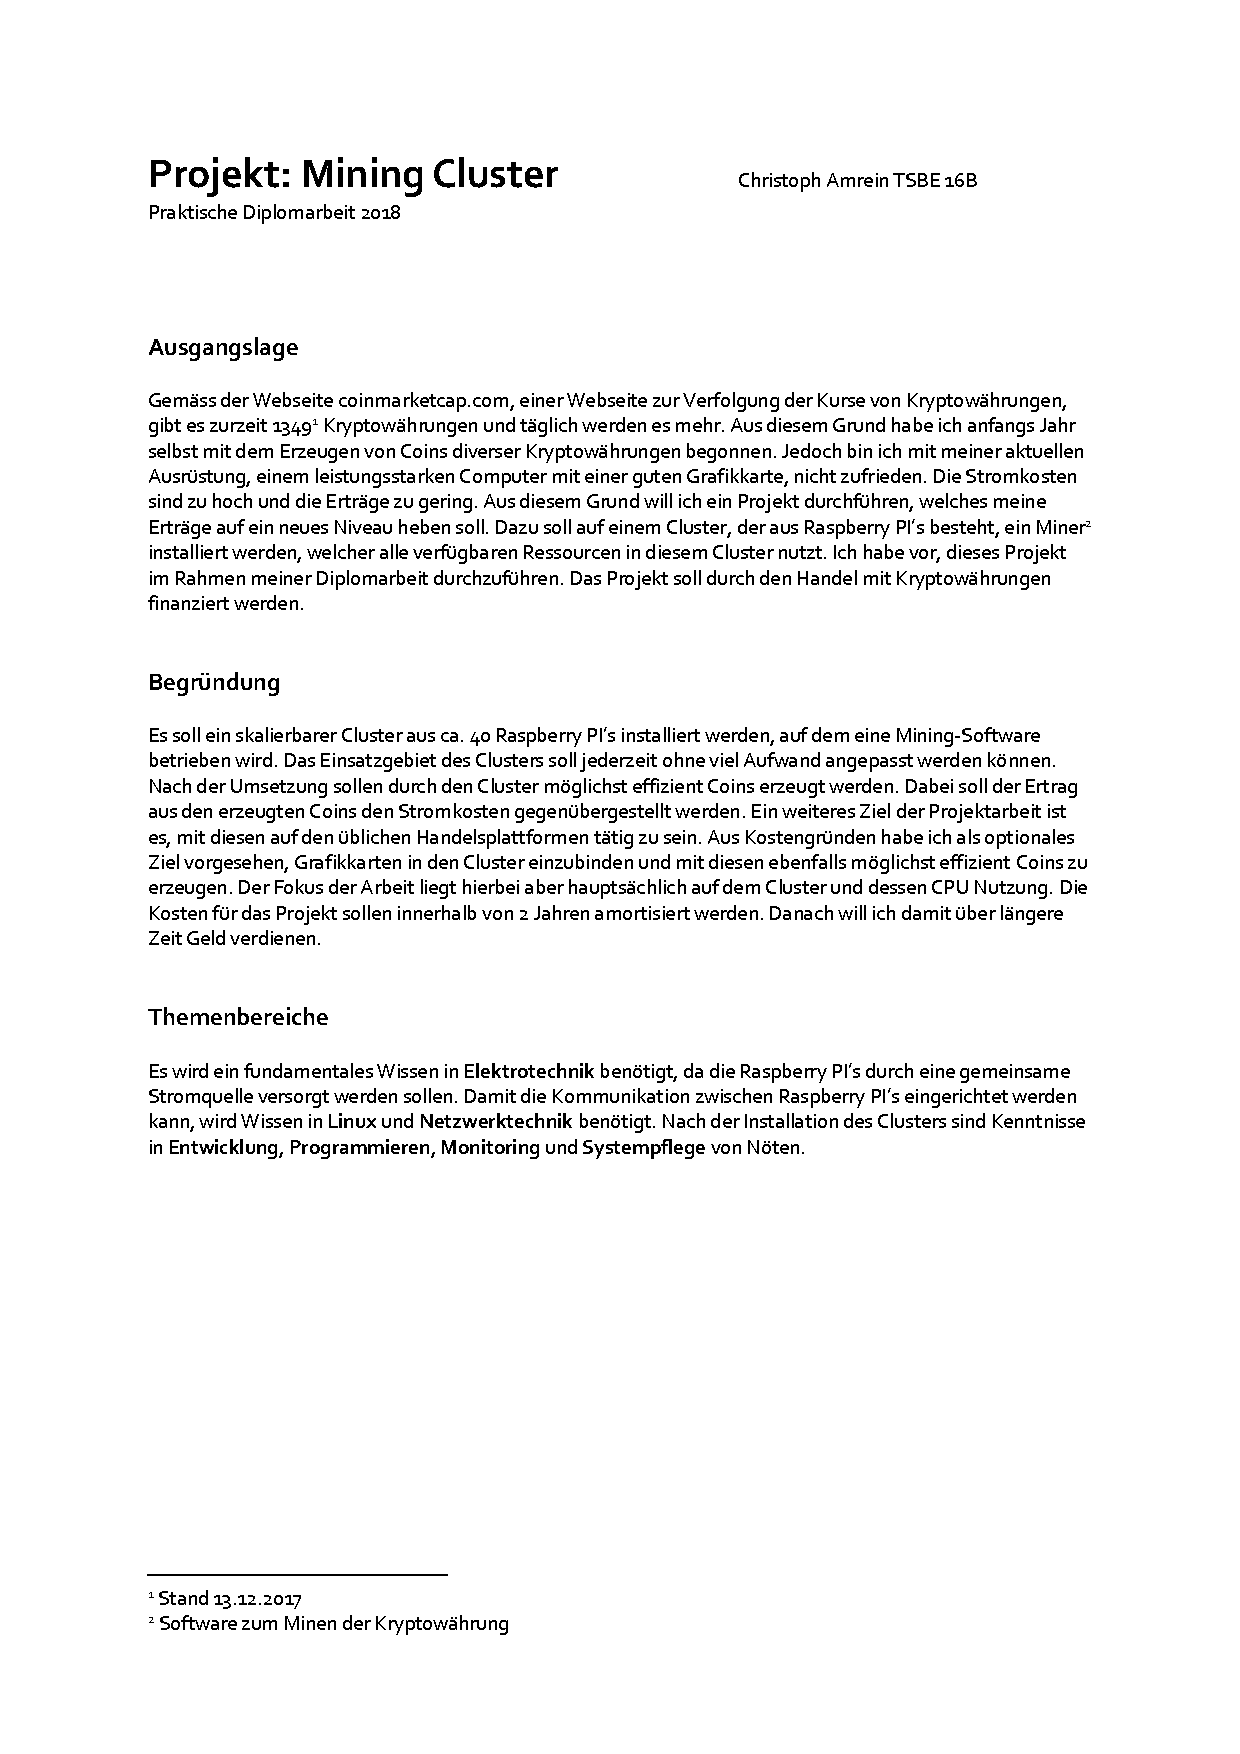
\includepdf[pages=1,scale=.8,pagecommand={\section{Diplomeingabe}\label{pdf:Diplomeingabe}},linktodoc=true]{Anhang/Diplomarbeit_Eingabe.pdf}
\includepdf[pages={2,3},scale=0.9,pagecommand={},linktodoc=true]{Anhang/Diplomarbeit_Eingabe.pdf}
% !TEX root = ../Diplombericht.tex
\section{Testfälle}
\subsection{Komponententests}
\begin{table}[H]
\centering
\begin{tabular}{|p{4cm}|p{4cm}|p{4cm}|p{4cm}|}
\hline
Bezeichnung & \textbf{K-001} & Management Node & Hostnamen / IP / MAC \\ \hline
Beschreibung & \multicolumn{3}{p{12cm}|}{Der Management Node wird auf die zugewiesene IP Adresse, MAC Adresse und den Hostnamen geprüft.} \\ \hline
Testvoraussetzung & \multicolumn{3}{p{12cm}|}{Der Management Node und der Testclient befinden sich im selben Netzwerk.} \\ \hline
Testschritte & \multicolumn{3}{p{12cm}|}{
- Management Node starten (Strom anschliessen).\newline
- 30 Sekunden warten.\newline
- Auf dem Testclient über Putty oder Shell mit dem Befehl \newline 
 \grqq nmap -sn 192.168.1.10\grqq \ eingeben.\newline
- Prüfen, ob der die Zuweisung gemäss Hostnamenkonzept richtig ist.} \\ \hline
Erwartetes Ergebnis & \multicolumn{3}{p{12cm}|}{Die Rückgabewerte (Hostnamen, IP- und MAC-Adresse) sollen identisch mit deren im Hostnamenkonzept sein.} \\\hline
\end{tabular}
\caption{Testfall K-001}
\label{Testfall K-001}
\end{table}

\begin{table}[H]
\centering
\begin{tabular}{|p{4cm}|p{4cm}|p{4cm}|p{4cm}|}
\hline
Bezeichnung & \textbf{K-002} & Management Node & Anmelden \\ \hline
Beschreibung & \multicolumn{3}{p{12cm}|}{Es wird getestet, ob der Management Node über das SSH Protokoll erreichbar ist.} \\ \hline
Testvoraussetzung & \multicolumn{3}{p{12cm}|}{Der Management Node und der Testclient befinden sich im selben Netzwerk.} \\ \hline
Testschritte & \multicolumn{3}{p{12cm}|}{
- Management Node starten (Strom anschliessen).\newline
- 30 Sekunden warten.\newline
- Auf dem Testclient über Putty oder Shell den Befehl \grqq ssh root@nebula\grqq \ \ eingeben. \newline
- Passwort eingeben.} \\ \hline
Erwartetes Ergebnis & \multicolumn{3}{p{12cm}|}{Der Zugriff auf den Management Node funktioniert.} \\\hline
\end{tabular}
\caption{Testfall K-002}
\label{Testfall K-002}
\end{table}

\begin{table}[H]
\centering
\begin{tabular}{|p{4cm}|p{4cm}|p{4cm}|p{4cm}|}
\hline
Bezeichnung & \textbf{K-003} & Compute Node c1 & Hostnamen / IP / MAC \\ \hline
Beschreibung & \multicolumn{3}{p{12cm}|}{Der Compute Node wird auf die zugewiesene IP Adresse, MAC Adresse und den Hostnamen geprüft.} \\ \hline
Testvoraussetzung & \multicolumn{3}{p{12cm}|}{Der Compute Node und der Testclient befinden sich im selben Netzwerk.} \\ \hline
Testschritte & \multicolumn{3}{p{12cm}|}{
- Compute Node starten (Strom anschliessen).\newline
- 3 Minuten warten.\newline
- Auf dem Testclient über Putty oder Shell mit dem Befehl \newline \grqq nmap -sn 192.168.1.11\grqq \ eingeben.\newline
- Prüfen, ob die Zuweisung gemäss Hostnamenkonzept richtig ist.} \\ \hline
Erwartetes Ergebnis & \multicolumn{3}{p{12cm}|}{Die Rückgabewerte (Hostnamen, IP- und MAC-Adresse) sollen identisch mit deren im Hostnamenkonzept sein.} \\\hline
\end{tabular}
\caption{Testfall K-003}
\label{Testfall K-003}
\end{table}


\begin{table}[H]
\centering
\begin{tabular}{|p{4cm}|p{4cm}|p{4cm}|p{4cm}|}
\hline
Bezeichnung & \textbf{K-004} & Compute Node c2 & Hostnamen / IP / MAC \\ \hline
Beschreibung & \multicolumn{3}{p{12cm}|}{Der Compute Node wird auf die zugewiesene IP Adresse, MAC Adresse und den Hostnamen geprüft.} \\ \hline
Testvoraussetzung & \multicolumn{3}{p{12cm}|}{Der Compute Node und der Testclient befinden sich im selben Netzwerk.} \\ \hline
Testschritte & \multicolumn{3}{p{12cm}|}{
- Compute Node starten (Strom anschliessen).\newline
- 3 Minuten warten.\newline
- Auf dem Testclient über Putty oder Shell mit dem Befehl \newline \grqq nmap -sn 192.168.1.12\grqq \ eingeben.\newline
- Prüfen, ob die Zuweisung gemäss Hostnamenkonzept richtig ist.} \\ \hline
Erwartetes Ergebnis & \multicolumn{3}{p{12cm}|}{Die Rückgabewerte (Hostnamen, IP- und MAC-Adresse) sollen identisch mit deren im Hostnamenkonzept sein.} \\\hline
\end{tabular}
\caption{Testfall K-004}
\label{Testfall K-004}
\end{table}


\begin{table}[H]
\centering
\begin{tabular}{|p{4cm}|p{4cm}|p{4cm}|p{4cm}|}
\hline
Bezeichnung & \textbf{K-005} & Compute Node c3 & Hostnamen / IP / MAC \\ \hline
Beschreibung & \multicolumn{3}{p{12cm}|}{Der Compute Node wird auf die zugewiesene IP Adresse, MAC Adresse und den Hostnamen geprüft.} \\ \hline
Testvoraussetzung & \multicolumn{3}{p{12cm}|}{Der Compute Node und der Testclient befinden sich im selben Netzwerk.} \\ \hline
Testschritte & \multicolumn{3}{p{12cm}|}{
- Compute Node starten (Strom anschliessen).\newline
- 3 Minuten warten.\newline
- Auf dem Testclient über Putty oder Shell mit dem Befehl \newline \grqq nmap -sn 192.168.1.13\grqq \ eingeben.\newline
- Prüfen, ob die Zuweisung gemäss Hostnamenkonzept richtig ist.} \\ \hline
Erwartetes Ergebnis & \multicolumn{3}{p{12cm}|}{Die Rückgabewerte (Hostnamen, IP- und MAC-Adresse) sollen identisch mit deren im Hostnamenkonzept sein.} \\\hline
\end{tabular}
\caption{Testfall K-005}
\label{Testfall K-005}
\end{table}


\begin{table}[H]
\centering
\begin{tabular}{|p{4cm}|p{4cm}|p{4cm}|p{4cm}|}
\hline
Bezeichnung & \textbf{K-006} & Compute Node c4 & Hostnamen / IP / MAC \\ \hline
Beschreibung & \multicolumn{3}{p{12cm}|}{Der Compute Node wird auf die zugewiesene IP Adresse, MAC Adresse und den Hostnamen geprüft.} \\ \hline
Testvoraussetzung & \multicolumn{3}{p{12cm}|}{Der Compute Node und der Testclient befinden sich im selben Netzwerk.} \\ \hline
Testschritte & \multicolumn{3}{p{12cm}|}{
- Compute Node starten (Strom anschliessen).\newline
- 3 Minuten warten.\newline
- Auf dem Testclient über Putty oder Shell mit dem Befehl \newline \grqq nmap -sn 192.168.1.14\grqq \ eingeben.\newline
- Prüfen, ob die Zuweisung gemäss Hostnamenkonzept richtig ist.} \\ \hline
Erwartetes Ergebnis & \multicolumn{3}{p{12cm}|}{Die Rückgabewerte (Hostnamen, IP- und MAC-Adresse) sollen identisch mit deren im Hostnamenkonzept sein.} \\\hline
\end{tabular}
\caption{Testfall K-006}
\label{Testfall K-006}
\end{table}


\begin{table}[H]
\centering
\begin{tabular}{|p{4cm}|p{4cm}|p{4cm}|p{4cm}|}
\hline
Bezeichnung & \textbf{K-007} & Compute Node c5 & Hostnamen / IP / MAC \\ \hline
Beschreibung & \multicolumn{3}{p{12cm}|}{Der Compute Node wird auf die zugewiesene IP Adresse, MAC Adresse und den Hostnamen geprüft.} \\ \hline
Testvoraussetzung & \multicolumn{3}{p{12cm}|}{Der Compute Node und der Testclient befinden sich im selben Netzwerk.} \\ \hline
Testschritte & \multicolumn{3}{p{12cm}|}{
- Compute Node starten (Strom anschliessen).\newline
- 3 Minuten warten.\newline
- Auf dem Testclient über Putty oder Shell mit dem Befehl \newline \grqq nmap -sn 192.168.1.15\grqq \ eingeben.\newline
- Prüfen, ob die Zuweisung gemäss Hostnamenkonzept richtig ist.} \\ \hline
Erwartetes Ergebnis & \multicolumn{3}{p{12cm}|}{Die Rückgabewerte (Hostnamen, IP- und MAC-Adresse) sollen identisch mit deren im Hostnamenkonzept sein.} \\\hline
\end{tabular}
\caption{Testfall K-007}
\label{Testfall K-007}
\end{table}


\begin{table}[H]
\centering
\begin{tabular}{|p{4cm}|p{4cm}|p{4cm}|p{4cm}|}
\hline
Bezeichnung & \textbf{K-008} & Compute Node c6 & Hostnamen / IP / MAC \\ \hline
Beschreibung & \multicolumn{3}{p{12cm}|}{Der Compute Node wird auf die zugewiesene IP Adresse, MAC Adresse und den Hostnamen geprüft.} \\ \hline
Testvoraussetzung & \multicolumn{3}{p{12cm}|}{Der Compute Node und der Testclient befinden sich im selben Netzwerk.} \\ \hline
Testschritte & \multicolumn{3}{p{12cm}|}{
- Compute Node starten (Strom anschliessen).\newline
- 3 Minuten warten.\newline
- Auf dem Testclient über Putty oder Shell mit dem Befehl \newline \grqq nmap -sn 192.168.1.16\grqq \ eingeben.\newline
- Prüfen, ob die Zuweisung gemäss Hostnamenkonzept richtig ist.} \\ \hline
Erwartetes Ergebnis & \multicolumn{3}{p{12cm}|}{Die Rückgabewerte (Hostnamen, IP- und MAC-Adresse) sollen identisch mit deren im Hostnamenkonzept sein.} \\\hline
\end{tabular}
\caption{Testfall K-008}
\label{Testfall K-008}
\end{table}


\begin{table}[H]
\centering
\begin{tabular}{|p{4cm}|p{4cm}|p{4cm}|p{4cm}|}
\hline
Bezeichnung & \textbf{K-009} & Compute Node c7 & Hostnamen / IP / MAC \\ \hline
Beschreibung & \multicolumn{3}{p{12cm}|}{Der Compute Node wird auf die zugewiesene IP Adresse, MAC Adresse und den Hostnamen geprüft.} \\ \hline
Testvoraussetzung & \multicolumn{3}{p{12cm}|}{Der Compute Node und der Testclient befinden sich im selben Netzwerk.} \\ \hline
Testschritte & \multicolumn{3}{p{12cm}|}{
- Compute Node starten (Strom anschliessen).\newline
- 3 Minuten warten.\newline
- Auf dem Testclient über Putty oder Shell mit dem Befehl \newline \grqq nmap -sn 192.168.1.17\grqq \ eingeben.\newline
- Prüfen, ob die Zuweisung gemäss Hostnamenkonzept richtig ist.} \\ \hline
Erwartetes Ergebnis & \multicolumn{3}{p{12cm}|}{Die Rückgabewerte (Hostnamen, IP- und MAC-Adresse) sollen identisch mit deren im Hostnamenkonzept sein.} \\\hline
\end{tabular}
\caption{Testfall K-009}
\label{Testfall K-009}
\end{table}


\begin{table}[H]
\centering
\begin{tabular}{|p{4cm}|p{4cm}|p{4cm}|p{4cm}|}
\hline
Bezeichnung & \textbf{K-010} & Compute Node c8 & Hostnamen / IP / MAC \\ \hline
Beschreibung & \multicolumn{3}{p{12cm}|}{Der Compute Node wird auf die zugewiesene IP Adresse, MAC Adresse und den Hostnamen geprüft.} \\ \hline
Testvoraussetzung & \multicolumn{3}{p{12cm}|}{Der Compute Node und der Testclient befinden sich im selben Netzwerk.} \\ \hline
Testschritte & \multicolumn{3}{p{12cm}|}{
- Compute Node starten (Strom anschliessen).\newline
- 3 Minuten warten.\newline
- Auf dem Testclient über Putty oder Shell mit dem Befehl \newline \grqq nmap -sn 192.168.1.18\grqq \ eingeben.\newline
- Prüfen, ob die Zuweisung gemäss Hostnamenkonzept richtig ist.} \\ \hline
Erwartetes Ergebnis & \multicolumn{3}{p{12cm}|}{Die Rückgabewerte (Hostnamen, IP- und MAC-Adresse) sollen identisch mit deren im Hostnamenkonzept sein.} \\\hline
\end{tabular}
\caption{Testfall K-010}
\label{Testfall K-010}
\end{table}



\begin{table}[H]
\centering
\begin{tabular}{|p{4cm}|p{4cm}|p{4cm}|p{4cm}|}
\hline
Bezeichnung & \textbf{K-011} & Compute Node c9 & Hostnamen / IP / MAC \\ \hline
Beschreibung & \multicolumn{3}{p{12cm}|}{Der Compute Node wird auf die zugewiesene IP Adresse, MAC Adresse und den Hostnamen geprüft.} \\ \hline
Testvoraussetzung & \multicolumn{3}{p{12cm}|}{Der Compute Node und der Testclient befinden sich im selben Netzwerk.} \\ \hline
Testschritte & \multicolumn{3}{p{12cm}|}{
- Compute Node starten (Strom anschliessen).\newline
- 3 Minuten warten.\newline
- Auf dem Testclient über Putty oder Shell mit dem Befehl \newline \grqq nmap -sn 192.168.1.19\grqq \ eingeben.\newline
- Prüfen, ob die Zuweisung gemäss Hostnamenkonzept richtig ist.} \\ \hline
Erwartetes Ergebnis & \multicolumn{3}{p{12cm}|}{Die Rückgabewerte (Hostnamen, IP- und MAC-Adresse) sollen identisch mit deren im Hostnamenkonzept sein.} \\\hline
\end{tabular}
\caption{Testfall K-011}
\label{Testfall K-011}
\end{table}


\begin{table}[H]
\centering
\begin{tabular}{|p{4cm}|p{4cm}|p{4cm}|p{4cm}|}
\hline
Bezeichnung & \textbf{K-012} & Compute Node c10 & Hostnamen / IP / MAC \\ \hline
Beschreibung & \multicolumn{3}{p{12cm}|}{Der Compute Node wird auf die zugewiesene IP Adresse, MAC Adresse und den Hostnamen geprüft.} \\ \hline
Testvoraussetzung & \multicolumn{3}{p{12cm}|}{Der Compute Node und der Testclient befinden sich im selben Netzwerk.} \\ \hline
Testschritte & \multicolumn{3}{p{12cm}|}{
- Compute Node starten (Strom anschliessen).\newline
- 3 Minuten warten.\newline
- Auf dem Testclient über Putty oder Shell mit dem Befehl \newline \grqq nmap -sn 192.168.1.20\grqq \ eingeben.\newline
- Prüfen, ob die Zuweisung gemäss Hostnamenkonzept richtig ist.} \\ \hline
Erwartetes Ergebnis & \multicolumn{3}{p{12cm}|}{Die Rückgabewerte (Hostnamen, IP- und MAC-Adresse) sollen identisch mit deren im Hostnamenkonzept sein.} \\\hline
\end{tabular}
\caption{Testfall K-012}
\label{Testfall K-012}
\end{table}


\begin{table}[H]
\centering
\begin{tabular}{|p{4cm}|p{4cm}|p{4cm}|p{4cm}|}
\hline
Bezeichnung & \textbf{K-013} & Compute Node c11 & Hostnamen / IP / MAC \\ \hline
Beschreibung & \multicolumn{3}{p{12cm}|}{Der Compute Node wird auf die zugewiesene IP Adresse, MAC Adresse und den Hostnamen geprüft.} \\ \hline
Testvoraussetzung & \multicolumn{3}{p{12cm}|}{Der Compute Node und der Testclient befinden sich im selben Netzwerk.} \\ \hline
Testschritte & \multicolumn{3}{p{12cm}|}{
- Compute Node starten (Strom anschliessen).\newline
- 3 Minuten warten.\newline
- Auf dem Testclient über Putty oder Shell mit dem Befehl \newline \grqq nmap -sn 192.168.1.21\grqq \ eingeben.\newline
- Prüfen, ob die Zuweisung gemäss Hostnamenkonzept richtig ist.} \\ \hline
Erwartetes Ergebnis & \multicolumn{3}{p{12cm}|}{Die Rückgabewerte (Hostnamen, IP- und MAC-Adresse) sollen identisch mit deren im Hostnamenkonzept sein.} \\\hline
\end{tabular}
\caption{Testfall K-013}
\label{Testfall K-013}
\end{table}


\begin{table}[H]
\centering
\begin{tabular}{|p{4cm}|p{4cm}|p{4cm}|p{4cm}|}
\hline
Bezeichnung & \textbf{K-014} & Compute Node c12 & Hostnamen / IP / MAC \\ \hline
Beschreibung & \multicolumn{3}{p{12cm}|}{Der Compute Node wird auf die zugewiesene IP Adresse, MAC Adresse und den Hostnamen geprüft.} \\ \hline
Testvoraussetzung & \multicolumn{3}{p{12cm}|}{Der Compute Node und der Testclient befinden sich im selben Netzwerk.} \\ \hline
Testschritte & \multicolumn{3}{p{12cm}|}{
- Compute Node starten (Strom anschliessen).\newline
- 3 Minuten warten.\newline
- Auf dem Testclient über Putty oder Shell mit dem Befehl \newline \grqq nmap -sn 192.168.1.22\grqq \ eingeben.\newline
- Prüfen, ob die Zuweisung gemäss Hostnamenkonzept richtig ist.} \\ \hline
Erwartetes Ergebnis & \multicolumn{3}{p{12cm}|}{Die Rückgabewerte (Hostnamen, IP- und MAC-Adresse) sollen identisch mit deren im Hostnamenkonzept sein.} \\\hline
\end{tabular}
\caption{Testfall K-014}
\label{Testfall K-014}
\end{table}


\begin{table}[H]
\centering
\begin{tabular}{|p{4cm}|p{4cm}|p{4cm}|p{4cm}|}
\hline
Bezeichnung & \textbf{K-015} & Compute Node c13 & Hostnamen / IP / MAC \\ \hline
Beschreibung & \multicolumn{3}{p{12cm}|}{Der Compute Node wird auf die zugewiesene IP Adresse, MAC Adresse und den Hostnamen geprüft.} \\ \hline
Testvoraussetzung & \multicolumn{3}{p{12cm}|}{Der Compute Node und der Testclient befinden sich im selben Netzwerk.} \\ \hline
Testschritte & \multicolumn{3}{p{12cm}|}{
- Compute Node starten (Strom anschliessen).\newline
- 3 Minuten warten.\newline
- Auf dem Testclient über Putty oder Shell mit dem Befehl \newline \grqq nmap -sn 192.168.1.23\grqq \ eingeben.\newline
- Prüfen, ob die Zuweisung gemäss Hostnamenkonzept richtig ist.} \\ \hline
Erwartetes Ergebnis & \multicolumn{3}{p{12cm}|}{Die Rückgabewerte (Hostnamen, IP- und MAC-Adresse) sollen identisch mit deren im Hostnamenkonzept sein.} \\\hline
\end{tabular}
\caption{Testfall K-015}
\label{Testfall K-015}
\end{table}


\begin{table}[H]
\centering
\begin{tabular}{|p{4cm}|p{4cm}|p{4cm}|p{4cm}|}
\hline
Bezeichnung & \textbf{K-016} & Compute Node c14 & Hostnamen / IP / MAC \\ \hline
Beschreibung & \multicolumn{3}{p{12cm}|}{Der Compute Node wird auf die zugewiesene IP Adresse, MAC Adresse und den Hostnamen geprüft.} \\ \hline
Testvoraussetzung & \multicolumn{3}{p{12cm}|}{Der Compute Node und der Testclient befinden sich im selben Netzwerk.} \\ \hline
Testschritte & \multicolumn{3}{p{12cm}|}{
- Compute Node starten (Strom anschliessen).\newline
- 3 Minuten warten.\newline
- Auf dem Testclient über Putty oder Shell mit dem Befehl \newline \grqq nmap -sn 192.168.1.24\grqq \ eingeben.\newline
- Prüfen, ob die Zuweisung gemäss Hostnamenkonzept richtig ist.} \\ \hline
Erwartetes Ergebnis & \multicolumn{3}{p{12cm}|}{Die Rückgabewerte (Hostnamen, IP- und MAC-Adresse) sollen identisch mit deren im Hostnamenkonzept sein.} \\\hline
\end{tabular}
\caption{Testfall K-016}
\label{Testfall K-016}
\end{table}


\begin{table}[H]
\centering
\begin{tabular}{|p{4cm}|p{4cm}|p{4cm}|p{4cm}|}
\hline
Bezeichnung & \textbf{K-017} & Compute Node c15 & Hostnamen / IP / MAC \\ \hline
Beschreibung & \multicolumn{3}{p{12cm}|}{Der Compute Node wird auf die zugewiesene IP Adresse, MAC Adresse und den Hostnamen geprüft.} \\ \hline
Testvoraussetzung & \multicolumn{3}{p{12cm}|}{Der Compute Node und der Testclient befinden sich im selben Netzwerk.} \\ \hline
Testschritte & \multicolumn{3}{p{12cm}|}{
- Compute Node starten (Strom anschliessen).\newline
- 3 Minuten warten.\newline
- Auf dem Testclient über Putty oder Shell mit dem Befehl \newline \grqq nmap -sn 192.168.1.25\grqq \ eingeben.\newline
- Prüfen, ob die Zuweisung gemäss Hostnamenkonzept richtig ist.} \\ \hline
Erwartetes Ergebnis & \multicolumn{3}{p{12cm}|}{Die Rückgabewerte (Hostnamen, IP- und MAC-Adresse) sollen identisch mit deren im Hostnamenkonzept sein.} \\\hline
\end{tabular}
\caption{Testfall K-017}
\label{Testfall K-017}
\end{table}


\begin{table}[H]
\centering
\begin{tabular}{|p{4cm}|p{4cm}|p{4cm}|p{4cm}|}
\hline
Bezeichnung & \textbf{K-018} & Compute Node c16 & Hostnamen / IP / MAC \\ \hline
Beschreibung & \multicolumn{3}{p{12cm}|}{Der Compute Node wird auf die zugewiesene IP Adresse, MAC Adresse und den Hostnamen geprüft.} \\ \hline
Testvoraussetzung & \multicolumn{3}{p{12cm}|}{Der Compute Node und der Testclient befinden sich im selben Netzwerk.} \\ \hline
Testschritte & \multicolumn{3}{p{12cm}|}{
- Compute Node starten (Strom anschliessen).\newline
- 3 Minuten warten.\newline
- Auf dem Testclient über Putty oder Shell mit dem Befehl \newline \grqq nmap -sn 192.168.1.26\grqq \ eingeben.\newline
- Prüfen, ob die Zuweisung gemäss Hostnamenkonzept richtig ist.} \\ \hline
Erwartetes Ergebnis & \multicolumn{3}{p{12cm}|}{Die Rückgabewerte (Hostnamen, IP- und MAC-Adresse) sollen identisch mit deren im Hostnamenkonzept sein.} \\\hline
\end{tabular}
\caption{Testfall K-018}
\label{Testfall K-018}
\end{table}


\begin{table}[H]
\centering
\begin{tabular}{|p{4cm}|p{4cm}|p{4cm}|p{4cm}|}
\hline
Bezeichnung & \textbf{K-019} & Compute Node c17 & Hostnamen / IP / MAC \\ \hline
Beschreibung & \multicolumn{3}{p{12cm}|}{Der Compute Node wird auf die zugewiesene IP Adresse, MAC Adresse und den Hostnamen geprüft.} \\ \hline
Testvoraussetzung & \multicolumn{3}{p{12cm}|}{Der Compute Node und der Testclient befinden sich im selben Netzwerk.} \\ \hline
Testschritte & \multicolumn{3}{p{12cm}|}{
- Compute Node starten (Strom anschliessen).\newline
- 3 Minuten warten.\newline
- Auf dem Testclient über Putty oder Shell mit dem Befehl \newline \grqq nmap -sn 192.168.1.27\grqq \ eingeben.\newline
- Prüfen, ob die Zuweisung gemäss Hostnamenkonzept richtig ist.} \\ \hline
Erwartetes Ergebnis & \multicolumn{3}{p{12cm}|}{Die Rückgabewerte (Hostnamen, IP- und MAC-Adresse) sollen identisch mit deren im Hostnamenkonzept sein.} \\\hline
\end{tabular}
\caption{Testfall K-019}
\label{Testfall K-019}
\end{table}


\begin{table}[H]
\centering
\begin{tabular}{|p{4cm}|p{4cm}|p{4cm}|p{4cm}|}
\hline
Bezeichnung & \textbf{K-020} & Compute Node c18 & Hostnamen / IP / MAC \\ \hline
Beschreibung & \multicolumn{3}{p{12cm}|}{Der Compute Node wird auf die zugewiesene IP Adresse, MAC Adresse und den Hostnamen geprüft.} \\ \hline
Testvoraussetzung & \multicolumn{3}{p{12cm}|}{Der Compute Node und der Testclient befinden sich im selben Netzwerk.} \\ \hline
Testschritte & \multicolumn{3}{p{12cm}|}{
- Compute Node starten (Strom anschliessen).\newline
- 3 Minuten warten.\newline
- Auf dem Testclient über Putty oder Shell mit dem Befehl \newline \grqq nmap -sn 192.168.1.28\grqq \ eingeben.\newline
- Prüfen, ob die Zuweisung gemäss Hostnamenkonzept richtig ist.} \\ \hline
Erwartetes Ergebnis & \multicolumn{3}{p{12cm}|}{Die Rückgabewerte (Hostnamen, IP- und MAC-Adresse) sollen identisch mit deren im Hostnamenkonzept sein.} \\\hline
\end{tabular}
\caption{Testfall K-020}
\label{Testfall K-020}
\end{table}


\begin{table}[H]
\centering
\begin{tabular}{|p{4cm}|p{4cm}|p{4cm}|p{4cm}|}
\hline
Bezeichnung & \textbf{K-021} & Compute Node c19 & Hostnamen / IP / MAC \\ \hline
Beschreibung & \multicolumn{3}{p{12cm}|}{Der Compute Node wird auf die zugewiesene IP Adresse, MAC Adresse und den Hostnamen geprüft.} \\ \hline
Testvoraussetzung & \multicolumn{3}{p{12cm}|}{Der Compute Node und der Testclient befinden sich im selben Netzwerk.} \\ \hline
Testschritte & \multicolumn{3}{p{12cm}|}{
- Compute Node starten (Strom anschliessen).\newline
- 3 Minuten warten.\newline
- Auf dem Testclient über Putty oder Shell mit dem Befehl \newline \grqq nmap -sn 192.168.1.29\grqq \ eingeben.\newline
- Prüfen, ob die Zuweisung gemäss Hostnamenkonzept richtig ist.} \\ \hline
Erwartetes Ergebnis & \multicolumn{3}{p{12cm}|}{Die Rückgabewerte (Hostnamen, IP- und MAC-Adresse) sollen identisch mit deren im Hostnamenkonzept sein.} \\\hline
\end{tabular}
\caption{Testfall K-021}
\label{Testfall K-021}
\end{table}



\begin{table}[H]
\centering
\begin{tabular}{|p{4cm}|p{4cm}|p{4cm}|p{4cm}|}
\hline
Bezeichnung & \textbf{K-022} & Compute Node c20 & Hostnamen / IP / MAC \\ \hline
Beschreibung & \multicolumn{3}{p{12cm}|}{Der Compute Node wird auf die zugewiesene IP Adresse, MAC Adresse und den Hostnamen geprüft.} \\ \hline
Testvoraussetzung & \multicolumn{3}{p{12cm}|}{Der Compute Node und der Testclient befinden sich im selben Netzwerk.} \\ \hline
Testschritte & \multicolumn{3}{p{12cm}|}{
- Compute Node starten (Strom anschliessen).\newline
- 3 Minuten warten.\newline
- Auf dem Testclient über Putty oder Shell mit dem Befehl \newline \grqq nmap -sn 192.168.1.30\grqq \ eingeben.\newline
- Prüfen, ob die Zuweisung gemäss Hostnamenkonzept richtig ist.} \\ \hline
Erwartetes Ergebnis & \multicolumn{3}{p{12cm}|}{Die Rückgabewerte (Hostnamen, IP- und MAC-Adresse) sollen identisch mit deren im Hostnamenkonzept sein.} \\\hline
\end{tabular}
\caption{Testfall K-022}
\label{Testfall K-022}
\end{table}


\begin{table}[H]
\centering
\begin{tabular}{|p{4cm}|p{4cm}|p{4cm}|p{4cm}|}
\hline
Bezeichnung & \textbf{K-023} & Compute Node c21 & Hostnamen / IP / MAC \\ \hline
Beschreibung & \multicolumn{3}{p{12cm}|}{Der Compute Node wird auf die zugewiesene IP Adresse, MAC Adresse und den Hostnamen geprüft.} \\ \hline
Testvoraussetzung & \multicolumn{3}{p{12cm}|}{Der Compute Node und der Testclient befinden sich im selben Netzwerk.} \\ \hline
Testschritte & \multicolumn{3}{p{12cm}|}{
- Compute Node starten (Strom anschliessen).\newline
- 3 Minuten warten.\newline
- Auf dem Testclient über Putty oder Shell mit dem Befehl \newline \grqq nmap -sn 192.168.1.31\grqq \ eingeben.\newline
- Prüfen, ob die Zuweisung gemäss Hostnamenkonzept richtig ist.} \\ \hline
Erwartetes Ergebnis & \multicolumn{3}{p{12cm}|}{Die Rückgabewerte (Hostnamen, IP- und MAC-Adresse) sollen identisch mit deren im Hostnamenkonzept sein.} \\\hline
\end{tabular}
\caption{Testfall K-023}
\label{Testfall K-023}
\end{table}


\begin{table}[H]
\centering
\begin{tabular}{|p{4cm}|p{4cm}|p{4cm}|p{4cm}|}
\hline
Bezeichnung & \textbf{K-024} & Compute Node c22 & Hostnamen / IP / MAC \\ \hline
Beschreibung & \multicolumn{3}{p{12cm}|}{Der Compute Node wird auf die zugewiesene IP Adresse, MAC Adresse und den Hostnamen geprüft.} \\ \hline
Testvoraussetzung & \multicolumn{3}{p{12cm}|}{Der Compute Node und der Testclient befinden sich im selben Netzwerk.} \\ \hline
Testschritte & \multicolumn{3}{p{12cm}|}{
- Compute Node starten (Strom anschliessen).\newline
- 3 Minuten warten.\newline
- Auf dem Testclient über Putty oder Shell mit dem Befehl \newline \grqq nmap -sn 192.168.1.32\grqq \ eingeben.\newline
- Prüfen, ob die Zuweisung gemäss Hostnamenkonzept richtig ist.} \\ \hline
Erwartetes Ergebnis & \multicolumn{3}{p{12cm}|}{Die Rückgabewerte (Hostnamen, IP- und MAC-Adresse) sollen identisch mit deren im Hostnamenkonzept sein.} \\\hline
\end{tabular}
\caption{Testfall K-024}
\label{Testfall K-024}
\end{table}


\begin{table}[H]
\centering
\begin{tabular}{|p{4cm}|p{4cm}|p{4cm}|p{4cm}|}
\hline
Bezeichnung & \textbf{K-025} & Compute Node c23 & Hostnamen / IP / MAC \\ \hline
Beschreibung & \multicolumn{3}{p{12cm}|}{Der Compute Node wird auf die zugewiesene IP Adresse, MAC Adresse und den Hostnamen geprüft.} \\ \hline
Testvoraussetzung & \multicolumn{3}{p{12cm}|}{Der Compute Node und der Testclient befinden sich im selben Netzwerk.} \\ \hline
Testschritte & \multicolumn{3}{p{12cm}|}{
- Compute Node starten (Strom anschliessen).\newline
- 3 Minuten warten.\newline
- Auf dem Testclient über Putty oder Shell mit dem Befehl \newline \grqq nmap -sn 192.168.1.33\grqq \ eingeben.\newline
- Prüfen, ob die Zuweisung gemäss Hostnamenkonzept richtig ist.} \\ \hline
Erwartetes Ergebnis & \multicolumn{3}{p{12cm}|}{Die Rückgabewerte (Hostnamen, IP- und MAC-Adresse) sollen identisch mit deren im Hostnamenkonzept sein.} \\\hline
\end{tabular}
\caption{Testfall K-025}
\label{Testfall K-025}
\end{table}


\begin{table}[H]
\centering
\begin{tabular}{|p{4cm}|p{4cm}|p{4cm}|p{4cm}|}
\hline
Bezeichnung & \textbf{K-026} & Compute Node c24 & Hostnamen / IP / MAC \\ \hline
Beschreibung & \multicolumn{3}{p{12cm}|}{Der Compute Node wird auf die zugewiesene IP Adresse, MAC Adresse und den Hostnamen geprüft.} \\ \hline
Testvoraussetzung & \multicolumn{3}{p{12cm}|}{Der Compute Node und der Testclient befinden sich im selben Netzwerk.} \\ \hline
Testschritte & \multicolumn{3}{p{12cm}|}{
- Compute Node starten (Strom anschliessen).\newline
- 3 Minuten warten.\newline
- Auf dem Testclient über Putty oder Shell mit dem Befehl \newline \grqq nmap -sn 192.168.1.34\grqq \ eingeben.\newline
- Prüfen, ob die Zuweisung gemäss Hostnamenkonzept richtig ist.} \\ \hline
Erwartetes Ergebnis & \multicolumn{3}{p{12cm}|}{Die Rückgabewerte (Hostnamen, IP- und MAC-Adresse) sollen identisch mit deren im Hostnamenkonzept sein.} \\\hline
\end{tabular}
\caption{Testfall K-026}
\label{Testfall K-026}
\end{table}


\begin{table}[H]
\centering
\begin{tabular}{|p{4cm}|p{4cm}|p{4cm}|p{4cm}|}
\hline
Bezeichnung & \textbf{K-027} & Compute Node c25 & Hostnamen / IP / MAC \\ \hline
Beschreibung & \multicolumn{3}{p{12cm}|}{Der Compute Node wird auf die zugewiesene IP Adresse, MAC Adresse und den Hostnamen geprüft.} \\ \hline
Testvoraussetzung & \multicolumn{3}{p{12cm}|}{Der Compute Node und der Testclient befinden sich im selben Netzwerk.} \\ \hline
Testschritte & \multicolumn{3}{p{12cm}|}{
- Compute Node starten (Strom anschliessen).\newline
- 3 Minuten warten.\newline
- Auf dem Testclient über Putty oder Shell mit dem Befehl \newline \grqq nmap -sn 192.168.1.35\grqq \ eingeben.\newline
- Prüfen, ob die Zuweisung gemäss Hostnamenkonzept richtig ist.} \\ \hline
Erwartetes Ergebnis & \multicolumn{3}{p{12cm}|}{Die Rückgabewerte (Hostnamen, IP- und MAC-Adresse) sollen identisch mit deren im Hostnamenkonzept sein.} \\\hline
\end{tabular}
\caption{Testfall K-027}
\label{Testfall K-027}
\end{table}


\begin{table}[H]
\centering
\begin{tabular}{|p{4cm}|p{4cm}|p{4cm}|p{4cm}|}
\hline
Bezeichnung & \textbf{K-028} & Compute Node c26 & Hostnamen / IP / MAC \\ \hline
Beschreibung & \multicolumn{3}{p{12cm}|}{Der Compute Node wird auf die zugewiesene IP Adresse, MAC Adresse und den Hostnamen geprüft.} \\ \hline
Testvoraussetzung & \multicolumn{3}{p{12cm}|}{Der Compute Node und der Testclient befinden sich im selben Netzwerk.} \\ \hline
Testschritte & \multicolumn{3}{p{12cm}|}{
- Compute Node starten (Strom anschliessen).\newline
- 3 Minuten warten.\newline
- Auf dem Testclient über Putty oder Shell mit dem Befehl \newline \grqq nmap -sn 192.168.1.36\grqq \ eingeben.\newline
- Prüfen, ob die Zuweisung gemäss Hostnamenkonzept richtig ist.} \\ \hline
Erwartetes Ergebnis & \multicolumn{3}{p{12cm}|}{Die Rückgabewerte (Hostnamen, IP- und MAC-Adresse) sollen identisch mit deren im Hostnamenkonzept sein.} \\\hline
\end{tabular}
\caption{Testfall K-028}
\label{Testfall K-028}
\end{table}


\begin{table}[H]
\centering
\begin{tabular}{|p{4cm}|p{4cm}|p{4cm}|p{4cm}|}
\hline
Bezeichnung & \textbf{K-029} & Compute Node c27 & Hostnamen / IP / MAC \\ \hline
Beschreibung & \multicolumn{3}{p{12cm}|}{Der Compute Node wird auf die zugewiesene IP Adresse, MAC Adresse und den Hostnamen geprüft.} \\ \hline
Testvoraussetzung & \multicolumn{3}{p{12cm}|}{Der Compute Node und der Testclient befinden sich im selben Netzwerk.} \\ \hline
Testschritte & \multicolumn{3}{p{12cm}|}{
- Compute Node starten (Strom anschliessen).\newline
- 3 Minuten warten.\newline
- Auf dem Testclient über Putty oder Shell mit dem Befehl \newline \grqq nmap -sn 192.168.1.37\grqq \ eingeben.\newline
- Prüfen, ob die Zuweisung gemäss Hostnamenkonzept richtig ist.} \\ \hline
Erwartetes Ergebnis & \multicolumn{3}{p{12cm}|}{Die Rückgabewerte (Hostnamen, IP- und MAC-Adresse) sollen identisch mit deren im Hostnamenkonzept sein.} \\\hline
\end{tabular}
\caption{Testfall K-029}
\label{Testfall K-029}
\end{table}


\begin{table}[H]
\centering
\begin{tabular}{|p{4cm}|p{4cm}|p{4cm}|p{4cm}|}
\hline
Bezeichnung & \textbf{K-030} & Compute Node c28 & Hostnamen / IP / MAC \\ \hline
Beschreibung & \multicolumn{3}{p{12cm}|}{Der Compute Node wird auf die zugewiesene IP Adresse, MAC Adresse und den Hostnamen geprüft.} \\ \hline
Testvoraussetzung & \multicolumn{3}{p{12cm}|}{Der Compute Node und der Testclient befinden sich im selben Netzwerk.} \\ \hline
Testschritte & \multicolumn{3}{p{12cm}|}{
- Compute Node starten (Strom anschliessen).\newline
- 3 Minuten warten.\newline
- Auf dem Testclient über Putty oder Shell mit dem Befehl \newline \grqq nmap -sn 192.168.1.38\grqq \ eingeben.\newline
- Prüfen, ob die Zuweisung gemäss Hostnamenkonzept richtig ist.} \\ \hline
Erwartetes Ergebnis & \multicolumn{3}{p{12cm}|}{Die Rückgabewerte (Hostnamen, IP- und MAC-Adresse) sollen identisch mit deren im Hostnamenkonzept sein.} \\\hline
\end{tabular}
\caption{Testfall K-030}
\label{Testfall K-030}
\end{table}


\begin{table}[H]
\centering
\begin{tabular}{|p{4cm}|p{4cm}|p{4cm}|p{4cm}|}
\hline
Bezeichnung & \textbf{K-031} & Compute Node c29 & Hostnamen / IP / MAC \\ \hline
Beschreibung & \multicolumn{3}{p{12cm}|}{Der Compute Node wird auf die zugewiesene IP Adresse, MAC Adresse und den Hostnamen geprüft.} \\ \hline
Testvoraussetzung & \multicolumn{3}{p{12cm}|}{Der Compute Node und der Testclient befinden sich im selben Netzwerk.} \\ \hline
Testschritte & \multicolumn{3}{p{12cm}|}{
- Compute Node starten (Strom anschliessen).\newline
- 3 Minuten warten.\newline
- Auf dem Testclient über Putty oder Shell mit dem Befehl \newline \grqq nmap -sn 192.168.1.39\grqq \ eingeben.\newline
- Prüfen, ob die Zuweisung gemäss Hostnamenkonzept richtig ist.} \\ \hline
Erwartetes Ergebnis & \multicolumn{3}{p{12cm}|}{Die Rückgabewerte (Hostnamen, IP- und MAC-Adresse) sollen identisch mit deren im Hostnamenkonzept sein.} \\\hline
\end{tabular}
\caption{Testfall K-031}
\label{Testfall K-031}
\end{table}


\begin{table}[H]
\centering
\begin{tabular}{|p{4cm}|p{4cm}|p{4cm}|p{4cm}|}
\hline
Bezeichnung & \textbf{K-032} & Compute Node c30 & Hostnamen / IP / MAC \\ \hline
Beschreibung & \multicolumn{3}{p{12cm}|}{Der Compute Node wird auf die zugewiesene IP Adresse, MAC Adresse und den Hostnamen geprüft.} \\ \hline
Testvoraussetzung & \multicolumn{3}{p{12cm}|}{Der Compute Node und der Testclient befinden sich im selben Netzwerk.} \\ \hline
Testschritte & \multicolumn{3}{p{12cm}|}{
- Compute Node starten (Strom anschliessen).\newline
- 3 Minuten warten.\newline
- Auf dem Testclient über Putty oder Shell mit dem Befehl \newline \grqq nmap -sn 192.168.1.40\grqq \ eingeben.\newline
- Prüfen, ob die Zuweisung gemäss Hostnamenkonzept richtig ist.} \\ \hline
Erwartetes Ergebnis & \multicolumn{3}{p{12cm}|}{Die Rückgabewerte (Hostnamen, IP- und MAC-Adresse) sollen identisch mit deren im Hostnamenkonzept sein.} \\\hline
\end{tabular}
\caption{Testfall K-032}
\label{Testfall K-032}
\end{table}



\begin{table}[H]
\centering
\begin{tabular}{|p{4cm}|p{4cm}|p{4cm}|p{4cm}|}
\hline
Bezeichnung & \textbf{K-033} & Compute Node c31 & Hostnamen / IP / MAC \\ \hline
Beschreibung & \multicolumn{3}{p{12cm}|}{Der Compute Node wird auf die zugewiesene IP Adresse, MAC Adresse und den Hostnamen geprüft.} \\ \hline
Testvoraussetzung & \multicolumn{3}{p{12cm}|}{Der Compute Node und der Testclient befinden sich im selben Netzwerk.} \\ \hline
Testschritte & \multicolumn{3}{p{12cm}|}{
- Compute Node starten (Strom anschliessen).\newline
- 3 Minuten warten.\newline
- Auf dem Testclient über Putty oder Shell mit dem Befehl \newline \grqq nmap -sn 192.168.1.41\grqq \ eingeben.\newline
- Prüfen, ob die Zuweisung gemäss Hostnamenkonzept richtig ist.} \\ \hline
Erwartetes Ergebnis & \multicolumn{3}{p{12cm}|}{Die Rückgabewerte (Hostnamen, IP- und MAC-Adresse) sollen identisch mit deren im Hostnamenkonzept sein.} \\\hline
\end{tabular}
\caption{Testfall K-033}
\label{Testfall K-033}
\end{table}


\begin{table}[H]
\centering
\begin{tabular}{|p{4cm}|p{4cm}|p{4cm}|p{4cm}|}
\hline
Bezeichnung & \textbf{K-034} & Compute Node c32 & Hostnamen / IP / MAC \\ \hline
Beschreibung & \multicolumn{3}{p{12cm}|}{Der Compute Node wird auf die zugewiesene IP Adresse, MAC Adresse und den Hostnamen geprüft.} \\ \hline
Testvoraussetzung & \multicolumn{3}{p{12cm}|}{Der Compute Node und der Testclient befinden sich im selben Netzwerk.} \\ \hline
Testschritte & \multicolumn{3}{p{12cm}|}{
- Compute Node starten (Strom anschliessen).\newline
- 3 Minuten warten.\newline
- Auf dem Testclient über Putty oder Shell mit dem Befehl \newline \grqq nmap -sn 192.168.1.42\grqq \ eingeben.\newline
- Prüfen, ob die Zuweisung gemäss Hostnamenkonzept richtig ist.} \\ \hline
Erwartetes Ergebnis & \multicolumn{3}{p{12cm}|}{Die Rückgabewerte (Hostnamen, IP- und MAC-Adresse) sollen identisch mit deren im Hostnamenkonzept sein.} \\\hline
\end{tabular}
\caption{Testfall K-034}
\label{Testfall K-034}
\end{table}


\begin{table}[H]
\centering
\begin{tabular}{|p{4cm}|p{4cm}|p{4cm}|p{4cm}|}
\hline
Bezeichnung & \textbf{K-035} & Compute Node c33 & Hostnamen / IP / MAC \\ \hline
Beschreibung & \multicolumn{3}{p{12cm}|}{Der Compute Node wird auf die zugewiesene IP Adresse, MAC Adresse und den Hostnamen geprüft.} \\ \hline
Testvoraussetzung & \multicolumn{3}{p{12cm}|}{Der Compute Node und der Testclient befinden sich im selben Netzwerk.} \\ \hline
Testschritte & \multicolumn{3}{p{12cm}|}{
- Compute Node starten (Strom anschliessen).\newline
- 3 Minuten warten.\newline
- Auf dem Testclient über Putty oder Shell mit dem Befehl \newline \grqq nmap -sn 192.168.1.43\grqq \ eingeben.\newline
- Prüfen, ob die Zuweisung gemäss Hostnamenkonzept richtig ist.} \\ \hline
Erwartetes Ergebnis & \multicolumn{3}{p{12cm}|}{Die Rückgabewerte (Hostnamen, IP- und MAC-Adresse) sollen identisch mit deren im Hostnamenkonzept sein.} \\\hline
\end{tabular}
\caption{Testfall K-035}
\label{Testfall K-035}
\end{table}


\begin{table}[H]
\centering
\begin{tabular}{|p{4cm}|p{4cm}|p{4cm}|p{4cm}|}
\hline
Bezeichnung & \textbf{K-036} & Compute Node c34 & Hostnamen / IP / MAC \\ \hline
Beschreibung & \multicolumn{3}{p{12cm}|}{Der Compute Node wird auf die zugewiesene IP Adresse, MAC Adresse und den Hostnamen geprüft.} \\ \hline
Testvoraussetzung & \multicolumn{3}{p{12cm}|}{Der Compute Node und der Testclient befinden sich im selben Netzwerk.} \\ \hline
Testschritte & \multicolumn{3}{p{12cm}|}{
- Compute Node starten (Strom anschliessen).\newline
- 3 Minuten warten.\newline
- Auf dem Testclient über Putty oder Shell mit dem Befehl \newline \grqq nmap -sn 192.168.1.44\grqq \ eingeben.\newline
- Prüfen, ob die Zuweisung gemäss Hostnamenkonzept richtig ist.} \\ \hline
Erwartetes Ergebnis & \multicolumn{3}{p{12cm}|}{Die Rückgabewerte (Hostnamen, IP- und MAC-Adresse) sollen identisch mit deren im Hostnamenkonzept sein.} \\\hline
\end{tabular}
\caption{Testfall K-036}
\label{Testfall K-036}
\end{table}


\begin{table}[H]
\centering
\begin{tabular}{|p{4cm}|p{4cm}|p{4cm}|p{4cm}|}
\hline
Bezeichnung & \textbf{K-037} & Compute Node c35 & Hostnamen / IP / MAC \\ \hline
Beschreibung & \multicolumn{3}{p{12cm}|}{Der Compute Node wird auf die zugewiesene IP Adresse, MAC Adresse und den Hostnamen geprüft.} \\ \hline
Testvoraussetzung & \multicolumn{3}{p{12cm}|}{Der Compute Node und der Testclient befinden sich im selben Netzwerk.} \\ \hline
Testschritte & \multicolumn{3}{p{12cm}|}{
- Compute Node starten (Strom anschliessen).\newline
- 3 Minuten warten.\newline
- Auf dem Testclient über Putty oder Shell mit dem Befehl \newline \grqq nmap -sn 192.168.1.45\grqq \ eingeben.\newline
- Prüfen, ob die Zuweisung gemäss Hostnamenkonzept richtig ist.} \\ \hline
Erwartetes Ergebnis & \multicolumn{3}{p{12cm}|}{Die Rückgabewerte (Hostnamen, IP- und MAC-Adresse) sollen identisch mit deren im Hostnamenkonzept sein.} \\\hline
\end{tabular}
\caption{Testfall K-037}
\label{Testfall K-037}
\end{table}


\begin{table}[H]
\centering
\begin{tabular}{|p{4cm}|p{4cm}|p{4cm}|p{4cm}|}
\hline
Bezeichnung & \textbf{K-038} & Compute Node c36 & Hostnamen / IP / MAC \\ \hline
Beschreibung & \multicolumn{3}{p{12cm}|}{Der Compute Node wird auf die zugewiesene IP Adresse, MAC Adresse und den Hostnamen geprüft.} \\ \hline
Testvoraussetzung & \multicolumn{3}{p{12cm}|}{Der Compute Node und der Testclient befinden sich im selben Netzwerk.} \\ \hline
Testschritte & \multicolumn{3}{p{12cm}|}{
- Compute Node starten (Strom anschliessen).\newline
- 3 Minuten warten.\newline
- Auf dem Testclient über Putty oder Shell mit dem Befehl \newline \grqq nmap -sn 192.168.1.46\grqq \ eingeben.\newline
- Prüfen, ob die Zuweisung gemäss Hostnamenkonzept richtig ist.} \\ \hline
Erwartetes Ergebnis & \multicolumn{3}{p{12cm}|}{Die Rückgabewerte (Hostnamen, IP- und MAC-Adresse) sollen identisch mit deren im Hostnamenkonzept sein.} \\\hline
\end{tabular}
\caption{Testfall K-038}
\label{Testfall K-038}
\end{table}


\begin{table}[H]
\centering
\begin{tabular}{|p{4cm}|p{4cm}|p{4cm}|p{4cm}|}
\hline
Bezeichnung & \textbf{K-039} & Compute Node c37 & Hostnamen / IP / MAC \\ \hline
Beschreibung & \multicolumn{3}{p{12cm}|}{Der Compute Node wird auf die zugewiesene IP Adresse, MAC Adresse und den Hostnamen geprüft.} \\ \hline
Testvoraussetzung & \multicolumn{3}{p{12cm}|}{Der Compute Node und der Testclient befinden sich im selben Netzwerk.} \\ \hline
Testschritte & \multicolumn{3}{p{12cm}|}{
- Compute Node starten (Strom anschliessen).\newline
- 3 Minuten warten.\newline
- Auf dem Testclient über Putty oder Shell mit dem Befehl \newline \grqq nmap -sn 192.168.1.47\grqq \ eingeben.\newline
- Prüfen, ob die Zuweisung gemäss Hostnamenkonzept richtig ist.} \\ \hline
Erwartetes Ergebnis & \multicolumn{3}{p{12cm}|}{Die Rückgabewerte (Hostnamen, IP- und MAC-Adresse) sollen identisch mit deren im Hostnamenkonzept sein.} \\\hline
\end{tabular}
\caption{Testfall K-039}
\label{Testfall K-039}
\end{table}


\begin{table}[H]
\centering
\begin{tabular}{|p{4cm}|p{4cm}|p{4cm}|p{4cm}|}
\hline
Bezeichnung & \textbf{K-040} & Compute Node c38 & Hostnamen / IP / MAC \\ \hline
Beschreibung & \multicolumn{3}{p{12cm}|}{Der Compute Node wird auf die zugewiesene IP Adresse, MAC Adresse und den Hostnamen geprüft.} \\ \hline
Testvoraussetzung & \multicolumn{3}{p{12cm}|}{Der Compute Node und der Testclient befinden sich im selben Netzwerk.} \\ \hline
Testschritte & \multicolumn{3}{p{12cm}|}{
- Compute Node starten (Strom anschliessen).\newline
- 3 Minuten warten.\newline
- Auf dem Testclient über Putty oder Shell mit dem Befehl \newline \grqq nmap -sn 192.168.1.48\grqq \ eingeben.\newline
- Prüfen, ob die Zuweisung gemäss Hostnamenkonzept richtig ist.} \\ \hline
Erwartetes Ergebnis & \multicolumn{3}{p{12cm}|}{Die Rückgabewerte (Hostnamen, IP- und MAC-Adresse) sollen identisch mit deren im Hostnamenkonzept sein.} \\\hline
\end{tabular}
\caption{Testfall K-040}
\label{Testfall K-040}
\end{table}


\begin{table}[H]
\centering
\begin{tabular}{|p{4cm}|p{4cm}|p{4cm}|p{4cm}|}
\hline
Bezeichnung & \textbf{K-041} & Compute Node c39 & Hostnamen / IP / MAC \\ \hline
Beschreibung & \multicolumn{3}{p{12cm}|}{Der Compute Node wird auf die zugewiesene IP Adresse, MAC Adresse und den Hostnamen geprüft.} \\ \hline
Testvoraussetzung & \multicolumn{3}{p{12cm}|}{Der Compute Node und der Testclient befinden sich im selben Netzwerk.} \\ \hline
Testschritte & \multicolumn{3}{p{12cm}|}{
- Compute Node starten (Strom anschliessen).\newline
- 3 Minuten warten.\newline
- Auf dem Testclient über Putty oder Shell mit dem Befehl \newline \grqq nmap -sn 192.168.1.49\grqq \ eingeben.\newline
- Prüfen, ob die Zuweisung gemäss Hostnamenkonzept richtig ist.} \\ \hline
Erwartetes Ergebnis & \multicolumn{3}{p{12cm}|}{Die Rückgabewerte (Hostnamen, IP- und MAC-Adresse) sollen identisch mit deren im Hostnamenkonzept sein.} \\\hline
\end{tabular}
\caption{Testfall K-041}
\label{Testfall K-041}
\end{table}


\begin{table}[H]
\centering
\begin{tabular}{|p{4cm}|p{4cm}|p{4cm}|p{4cm}|}
\hline
Bezeichnung & \textbf{K-042} & Compute Node c40 & Hostnamen / IP / MAC \\ \hline
Beschreibung & \multicolumn{3}{p{12cm}|}{Der Compute Node wird auf die zugewiesene IP Adresse, MAC Adresse und den Hostnamen geprüft.} \\ \hline
Testvoraussetzung & \multicolumn{3}{p{12cm}|}{Der Compute Node und der Testclient befinden sich im selben Netzwerk.} \\ \hline
Testschritte & \multicolumn{3}{p{12cm}|}{
- Compute Node starten (Strom anschliessen).\newline
- 3 Minuten warten.\newline
- Auf dem Testclient über Putty oder Shell mit dem Befehl \newline \grqq nmap -sn 192.168.1.50\grqq \ eingeben.\newline
- Prüfen, ob die Zuweisung gemäss Hostnamenkonzept richtig ist.} \\ \hline
Erwartetes Ergebnis & \multicolumn{3}{p{12cm}|}{Die Rückgabewerte (Hostnamen, IP- und MAC-Adresse) sollen identisch mit deren im Hostnamenkonzept sein.} \\\hline
\end{tabular}
\caption{Testfall K-042}
\label{Testfall K-042}
\end{table}



\begin{table}[H]
\centering
\begin{tabular}{|p{4cm}|p{4cm}|p{4cm}|p{4cm}|}
\hline
Bezeichnung & \textbf{K-043} & Compute Node c41 & Hostnamen / IP / MAC \\ \hline
Beschreibung & \multicolumn{3}{p{12cm}|}{Der Compute Node wird auf die zugewiesene IP Adresse, MAC Adresse und den Hostnamen geprüft.} \\ \hline
Testvoraussetzung & \multicolumn{3}{p{12cm}|}{Der Compute Node und der Testclient befinden sich im selben Netzwerk.} \\ \hline
Testschritte & \multicolumn{3}{p{12cm}|}{
- Compute Node starten (Strom anschliessen).\newline
- 3 Minuten warten.\newline
- Auf dem Testclient über Putty oder Shell mit dem Befehl \newline \grqq nmap -sn 192.168.1.51\grqq \ eingeben.\newline
- Prüfen, ob die Zuweisung gemäss Hostnamenkonzept richtig ist.} \\ \hline
Erwartetes Ergebnis & \multicolumn{3}{p{12cm}|}{Die Rückgabewerte (Hostnamen, IP- und MAC-Adresse) sollen identisch mit deren im Hostnamenkonzept sein.} \\\hline
\end{tabular}
\caption{Testfall K-043}
\label{Testfall K-043}
\end{table}


\begin{table}[H]
\centering
\begin{tabular}{|p{4cm}|p{4cm}|p{4cm}|p{4cm}|}
\hline
Bezeichnung & \textbf{K-044} & Compute Node c42 & Hostnamen / IP / MAC \\ \hline
Beschreibung & \multicolumn{3}{p{12cm}|}{Der Compute Node wird auf die zugewiesene IP Adresse, MAC Adresse und den Hostnamen geprüft.} \\ \hline
Testvoraussetzung & \multicolumn{3}{p{12cm}|}{Der Compute Node und der Testclient befinden sich im selben Netzwerk.} \\ \hline
Testschritte & \multicolumn{3}{p{12cm}|}{
- Compute Node starten (Strom anschliessen).\newline
- 3 Minuten warten.\newline
- Auf dem Testclient über Putty oder Shell mit dem Befehl \newline \grqq nmap -sn 192.168.1.52\grqq \ eingeben.\newline
- Prüfen, ob die Zuweisung gemäss Hostnamenkonzept richtig ist.} \\ \hline
Erwartetes Ergebnis & \multicolumn{3}{p{12cm}|}{Die Rückgabewerte (Hostnamen, IP- und MAC-Adresse) sollen identisch mit deren im Hostnamenkonzept sein.} \\\hline
\end{tabular}
\caption{Testfall K-044}
\label{Testfall K-044}
\end{table}


\begin{table}[H]
\centering
\begin{tabular}{|p{4cm}|p{4cm}|p{4cm}|p{4cm}|}
\hline
Bezeichnung & \textbf{K-045} & Compute Node c43 & Hostnamen / IP / MAC \\ \hline
Beschreibung & \multicolumn{3}{p{12cm}|}{Der Compute Node wird auf die zugewiesene IP Adresse, MAC Adresse und den Hostnamen geprüft.} \\ \hline
Testvoraussetzung & \multicolumn{3}{p{12cm}|}{Der Compute Node und der Testclient befinden sich im selben Netzwerk.} \\ \hline
Testschritte & \multicolumn{3}{p{12cm}|}{
- Compute Node starten (Strom anschliessen).\newline
- 3 Minuten warten.\newline
- Auf dem Testclient über Putty oder Shell mit dem Befehl \newline \grqq nmap -sn 192.168.1.53\grqq \ eingeben.\newline
- Prüfen, ob die Zuweisung gemäss Hostnamenkonzept richtig ist.} \\ \hline
Erwartetes Ergebnis & \multicolumn{3}{p{12cm}|}{Die Rückgabewerte (Hostnamen, IP- und MAC-Adresse) sollen identisch mit deren im Hostnamenkonzept sein.} \\\hline
\end{tabular}
\caption{Testfall K-045}
\label{Testfall K-045}
\end{table}


\begin{table}[H]
\centering
\begin{tabular}{|p{4cm}|p{4cm}|p{4cm}|p{4cm}|}
\hline
Bezeichnung & \textbf{K-046} & Compute Node c44 & Hostnamen / IP / MAC \\ \hline
Beschreibung & \multicolumn{3}{p{12cm}|}{Der Compute Node wird auf die zugewiesene IP Adresse, MAC Adresse und den Hostnamen geprüft.} \\ \hline
Testvoraussetzung & \multicolumn{3}{p{12cm}|}{Der Compute Node und der Testclient befinden sich im selben Netzwerk.} \\ \hline
Testschritte & \multicolumn{3}{p{12cm}|}{
- Compute Node starten (Strom anschliessen).\newline
- 3 Minuten warten.\newline
- Auf dem Testclient über Putty oder Shell mit dem Befehl \newline \grqq nmap -sn 192.168.1.54\grqq \ eingeben.\newline
- Prüfen, ob die Zuweisung gemäss Hostnamenkonzept richtig ist.} \\ \hline
Erwartetes Ergebnis & \multicolumn{3}{p{12cm}|}{Die Rückgabewerte (Hostnamen, IP- und MAC-Adresse) sollen identisch mit deren im Hostnamenkonzept sein.} \\\hline
\end{tabular}
\caption{Testfall K-046}
\label{Testfall K-046}
\end{table}


\begin{table}[H]
\centering
\begin{tabular}{|p{4cm}|p{4cm}|p{4cm}|p{4cm}|}
\hline
Bezeichnung & \textbf{K-047} & Compute Node c45 & Hostnamen / IP / MAC \\ \hline
Beschreibung & \multicolumn{3}{p{12cm}|}{Der Compute Node wird auf die zugewiesene IP Adresse, MAC Adresse und den Hostnamen geprüft.} \\ \hline
Testvoraussetzung & \multicolumn{3}{p{12cm}|}{Der Compute Node und der Testclient befinden sich im selben Netzwerk.} \\ \hline
Testschritte & \multicolumn{3}{p{12cm}|}{
- Compute Node starten (Strom anschliessen).\newline
- 3 Minuten warten.\newline
- Auf dem Testclient über Putty oder Shell mit dem Befehl \newline \grqq nmap -sn 192.168.1.55\grqq \ eingeben.\newline
- Prüfen, ob die Zuweisung gemäss Hostnamenkonzept richtig ist.} \\ \hline
Erwartetes Ergebnis & \multicolumn{3}{p{12cm}|}{Die Rückgabewerte (Hostnamen, IP- und MAC-Adresse) sollen identisch mit deren im Hostnamenkonzept sein.} \\\hline
\end{tabular}
\caption{Testfall K-047}
\label{Testfall K-047}
\end{table}

\begin{table}[H]
\centering
\begin{tabular}{|p{4cm}|p{4cm}|p{4cm}|p{4cm}|}
\hline
Bezeichnung & \textbf{K-048} & NAS & Erreichbarkeit \\ \hline
Beschreibung & \multicolumn{3}{p{12cm}|}{Das NAS soll auf die Erreichbarkeit geprüft werden.} \\ \hline
Testvoraussetzung & \multicolumn{3}{p{12cm}|}{Das NAS ist am Netzwerk angeschlossen.} \\ \hline
Testschritte & \multicolumn{3}{p{12cm}|}{Den Befehl \grqq ping 192.168.1.129\grqq \ \ auf dem Testclient ausführen und 2 Versuche abwarten.} \\ \hline
Erwartetes Ergebnis & \multicolumn{3}{p{12cm}|}{Das NAS antwortet auf den Ping befehl mit: \grqq 2 packets transmitted, 2 received, 0\% packet loss\grqq. } \\\hline
\end{tabular}
\caption{Testfall K-048}
\label{Testfall K-048}
\end{table}


\subsection{Integrationstests}

\begin{table}[H]
\centering
\begin{tabular}{|p{4cm}|p{4cm}|p{4cm}|p{4cm}|}
\hline
Bezeichnung & \textbf{I-001} & Compute Nodes & Internet Zugang \\ \hline
Beschreibung & \multicolumn{3}{p{12cm}|}{Es wird getestet, ob alle Compute Nodes auf das Internet zugreifen können.} \\ \hline
Testvoraussetzung & \multicolumn{3}{p{12cm}|}{Das Routing ist eingerichtet.} \\ \hline
Testschritte & \multicolumn{3}{p{12cm}|}{
- Den Befehl \grqq  pdsh -w c[1-45] ping -c 1 google.de\grqq \ auf dem Management Node eingeben.} \\ \hline
Erwartetes Ergebnis & \multicolumn{3}{p{12cm}|}{Der Rückgabewert muss pro Compute Node die Ausgabe \grqq 1 packets transmitted, 1 received, 0\% packet loss\grqq \ \ beinhalten. Damit der Test erfolgreich war.
} \\\hline
\end{tabular}
\caption{Testfall I-001}
\label{Testfall I-001}
\end{table}

\begin{table}[H]
\centering
\begin{tabular}{|p{4cm}|p{4cm}|p{4cm}|p{4cm}|}
\hline
Bezeichnung & \textbf{I-002} & NAS / Management Node & Mountpoint \\ \hline
Beschreibung & \multicolumn{3}{p{12cm}|}{Es wird getestet, ob der Management Node sich automatisch bei einem Systemstart mit dem Netzwerkshare verbindet.} \\ \hline
Testvoraussetzung & \multicolumn{3}{p{12cm}|}{Der fstab-Eintrag muss vorhanden sein.} \\ \hline
Testschritte & \multicolumn{3}{p{12cm}|}{
- Management Node starten.\newline
- Auf dem Management Node anmelden.\newline
- Den Befehl \grqq ls -l /media/nebula\_data/ | wc -l\grqq\ eingeben.
} \\ \hline
Erwartetes Ergebnis & \multicolumn{3}{p{12cm}|}{Die Ausgabe des Befehls muss einen grösseren Wert als \grqq 1\grqq \  zurückgeben.} \\\hline
\end{tabular}
\caption{Testfall I-002}
\label{Testfall I-002}
\end{table}

\begin{table}[H]
\centering
\begin{tabular}{|p{4cm}|p{4cm}|p{4cm}|p{4cm}|}
\hline
Bezeichnung & \textbf{I-003} & NAS / Compute Nodes & Mountpoint \\ \hline
Beschreibung & \multicolumn{3}{p{12cm}|}{Es wird getestet, ob die Compute Nodes sich automatisch bei einem Systemstart mit dem Netzwerkshare verbinden.} \\ \hline
Testvoraussetzung & \multicolumn{3}{p{12cm}|}{Der fstab-Eintrag muss vorhanden sein.} \\ \hline
Testschritte & \multicolumn{3}{p{12cm}|}{
- Compute Nodes starten.\newline
- Auf dem Management Node anmelden.\newline
- Den Befehl \grqq pdsh -w c[1-45] ls -l /media/nebula\_data/ | wc -l\grqq \ eingeben.
} \\ \hline
Erwartetes Ergebnis & \multicolumn{3}{p{12cm}|}{Die Ausgabe des Befehls muss jeweils einen grösseren Wert als \grqq 1\grqq zurückgeben.} \\\hline
\end{tabular}
\caption{Testfall I-003}
\label{Testfall I-003}
\end{table}

\begin{table}[H]
\centering
\begin{tabular}{|p{4cm}|p{4cm}|p{4cm}|p{4cm}|}
\hline
Bezeichnung & \textbf{I-004} & Cluster & Wiederaufbau \\ \hline
Beschreibung & \multicolumn{3}{p{12cm}|}{Es wird getestet, ob der Cluster in einem Raum innerhalb von 15 Minuten wiederaufgebaut werden kann.} \\ \hline
Testvoraussetzung & \multicolumn{3}{p{12cm}|}{Cluster ist kompakt aufgebaut.} \\ \hline
Testschritte & \multicolumn{3}{p{12cm}|}{
- Cluster herunterfahren.\newline
- Externe physische Verbindungen trennen.\newline
- Cluster in ein anderes Zimmer verschieben und wiederaufbauen (selbes Netzwerk).
} \\ \hline
Erwartetes Ergebnis & \multicolumn{3}{p{12cm}|}{Der Wiederaufbau soll nicht länger als 15 Minuten dauern.} \\\hline
\end{tabular}
\caption{Testfall I-004}
\label{Testfall I-004}
\end{table}

\subsection{Systemtests}
\begin{table}[H]
\centering
\begin{tabular}{|p{4cm}|p{4cm}|p{4cm}|p{4cm}|}
\hline
Bezeichnung & \textbf{S-001} & Compute Nodes & CPU Last \\ \hline
Beschreibung & \multicolumn{3}{p{12cm}|}{Es wird geprüft, ob die CPU während des Schürfens der Kryptowährungen zu über 90\% beansprucht wird. } \\ \hline
Testvoraussetzung & \multicolumn{3}{p{12cm}|}{Der Cluster muss am Schürfen einer Kryptowährung sein. Dazu muss er bereits 15 Minuten am Schürfen sein, bevor mit dem Test begonnen werden kann.} \\ \hline
Testschritte & \multicolumn{3}{p{12cm}|}{
Die Tests finden vom Management Node aus statt.\newline
- Den Befehl \grqq pdsh -w c[1-45] uptime\grqq \ eingeben. \newline
- Alternativ kann man sich auf jeden Compute Node anmelden und den Befehl \grqq top\grqq \ eingeben. 
} \\ \hline
Erwartetes Ergebnis & \multicolumn{3}{p{12cm}|}{Die Loadaverage-Werte überschreiten jeweils den Wert 1, die Ausgabe sollte in etwa so aussehen: \newline  load average: 4.18, 2.44, 1.16} \\\hline
\end{tabular}
\caption{Testfall S-001}
\label{Testfall S-001}
\end{table}

\begin{table}[H]
\centering
\begin{tabular}{|p{4cm}|p{4cm}|p{4cm}|p{4cm}|}
\hline
Bezeichnung & \textbf{S-002} & Nodes & Nagios Monitoring \\ \hline
Beschreibung & \multicolumn{3}{p{12cm}|}{Es wird geprüft, ob alle Nodes von Nagios überwacht werden. } \\ \hline
Testvoraussetzung & \multicolumn{3}{p{12cm}|}{Alle Nodes müssen einmal in Betrieb gewesen sein.} \\ \hline
Testschritte & \multicolumn{3}{p{12cm}|}{
- \url{http://nebula/nagios} aufrufen. \newline
- Bei Nagios anmelden. \newline
- Auf den Reiter \grqq Hosts\grqq \  klicken.
} \\ \hline
Erwartetes Ergebnis & \multicolumn{3}{p{12cm}|}{Es werden alle Nodes aufgelistet. Unabhängig des Status, ob der Node in Betrieb ist oder nicht.} \\\hline
\end{tabular}
\caption{Testfall S-002}
\label{Testfall S-002}
\end{table}

\begin{table}[H]
\centering
\begin{tabular}{|p{4cm}|p{4cm}|p{4cm}|p{4cm}|}
\hline
Bezeichnung & \textbf{S-003} & Nodes & Nagios Alarmierung \\ \hline
Beschreibung & \multicolumn{3}{p{12cm}|}{Bei aufgetretenen Problemen soll Nagios eine E-Mail versenden.} \\ \hline
Testvoraussetzung & \multicolumn{3}{p{12cm}|}{Der Cluster muss in Betrieb sein.} \\ \hline
Testschritte & \multicolumn{3}{p{12cm}|}{
- Strom von Node c1 trennen. \newline
- 5 Minuten warten. \newline
- Email prüfen (christoph.amrein86@gmail.com).
} \\ \hline
Erwartetes Ergebnis & \multicolumn{3}{p{12cm}|}{Es trifft eine Alarmierungs-Email ein.} \\\hline
\end{tabular}
\caption{Testfall S-003}
\label{Testfall S-003}
\end{table}

\begin{table}[H]
\centering
\begin{tabular}{|p{4cm}|p{4cm}|p{4cm}|p{4cm}|}
\hline
Bezeichnung & \textbf{S-004} & Nodes & Ganglia Monitoring \\ \hline
Beschreibung & \multicolumn{3}{p{12cm}|}{Es wird geprüft, ob alle Nodes von Ganglia gemonitored werden. } \\ \hline
Testvoraussetzung & \multicolumn{3}{p{12cm}|}{Alle Nodes müssen einmal in Betrieb gewesen sein.} \\ \hline
Testschritte & \multicolumn{3}{p{12cm}|}{
- \url{http://nebula/ganglia} aufrufen. \newline
- Quelle \grqq  Nebula\grqq \ auswählen.
} \\ \hline
Erwartetes Ergebnis & \multicolumn{3}{p{12cm}|}{Es werden alle Nodes aufgelistet. } \\\hline
\end{tabular}
\caption{Testfall S-004}
\label{Testfall S-004}
\end{table}

\begin{table}[H]
\centering
\begin{tabular}{|p{4cm}|p{4cm}|p{4cm}|p{4cm}|}
\hline
Bezeichnung & \textbf{S-005} & Nodes & Cluster Jobs \\ \hline
Beschreibung & \multicolumn{3}{p{12cm}|}{Es wird geprüft, ob Jobs auf dem Cluster laufen. } \\ \hline
Testvoraussetzung & \multicolumn{3}{p{12cm}|}{Der Cluster muss in Betrieb sein.} \\ \hline
Testschritte & \multicolumn{3}{p{12cm}|}{
Auf dem Management Node sind folgende Befehle abzusetzen: \newline
- \grqq mpicc -O3 /opt/ohpc/pub/examples/mpi/hello.c\grqq \newline
- \grqq srun -n 8 -N 2 --pty /bin/bash\grqq \newline
- \grqq squeue\grqq
} \\ \hline
Erwartetes Ergebnis & \multicolumn{3}{p{12cm}|}{Der Job wird in der Queue angezeigt und ist 2 Nodes zugewiesen. } \\\hline
\end{tabular}
\caption{Testfall S-005}
\label{Testfall S-005}
\end{table}


\begin{table}[H]
\centering
\begin{tabular}{|p{4cm}|p{4cm}|p{4cm}|p{4cm}|}
\hline
Bezeichnung & \textbf{S-006} & Nodes & Schürfen \\ \hline
Beschreibung & \multicolumn{3}{p{12cm}|}{Es wird geprüft, ob über den Cluster Kryptowährung über einen Job geschürft werden kann. } \\ \hline
Testvoraussetzung & \multicolumn{3}{p{12cm}|}{Der Cluster muss in Betrieb sein.} \\ \hline
Testschritte & \multicolumn{3}{p{12cm}|}{
Auf dem Management Node sind folgende Befehle als root abzusetzen: \newline
- \grqq cd /opt/miners/tkinjo\grqq \newline
- \grqq srun --nodes=40-45 --ntasks=40 --cpus-per-task=4 ./cpuminer  -a cryptonight -o stratum+tcp://xdn.pool.minergate.com:45620 -u x -p x\grqq \newline
} \\ \hline
Erwartetes Ergebnis & \multicolumn{3}{p{12cm}|}{Es soll direkt in der Shell die Ausgabe des Miners ausgegeben werden. } \\\hline
\end{tabular}
\caption{Testfall S-006}
\label{Testfall S-006}
\end{table}
% !TEX root = ../Diplombericht.tex
\section{Testprotokoll}
\subsection{Komponententests}
\begin{table}[H]
\centering
\begin{tabular}{p{4.5cm}p{11.5cm}}
\hline
\cellcolor{heading}\textbf{Test-ID:} & K-001 \\\hline
\cellcolor{heading}\textbf{Testobjekt} & Management Node \\\hline
\cellcolor{heading}\textbf{Testschritte} & 
- Management Node starten (Strom anschliessen).\newline
- 30 Sekunden warten.\newline
- Auf dem Testclient über Putty oder Shell mit dem Befehl \newline \grqq nmap -sn 192.168.1.10 \grqq eingeben.\newline
- Prüfen, ob die Zuweisung gemäss Hostnamenkonzept richtig ist. \\\hline
\cellcolor{heading}\textbf{Erwartetes Ergebnis} & Hostname = nebula \newline
IP = 192.168.1.10 \newline
MAC = B8:27:EB:32:A9:1C \\\hline
\cellcolor{heading}\textbf{Tatsächliches Ergebnis} &
Nmap scan report for nebula.home (192.168.1.10)\newline
MAC Address: B8:27:EB:32:A9:1C (Raspberry Pi Foundation)\newline
Nmap done: 1 IP address (1 host up) scanned in 0.26 seconds)  \\\hline
\cellcolor{heading}\textbf{Tester} & Christoph Amrein  \\\hline
\cellcolor{heading}\textbf{Datum des Tests} & 21.05.2018  \\\hline
\cellcolor{heading}\textbf{Testergebnis \newline (Fehlerklasse)} & 1 - Fehlerfrei, die Erwartungen sind erfüllt. \\\hline
\cellcolor{heading}\textbf{Fehlerbeschreibung} &   \\\hline
\end{tabular}
\caption{K-001 Protokoll}
\end{table}

\begin{table}[H]
\centering
\begin{tabular}{p{4.5cm}p{11.5cm}}
\hline
\cellcolor{heading}\textbf{Test-ID:} & K-002 \\\hline
\cellcolor{heading}\textbf{Testobjekt} & Management Node \\\hline
\cellcolor{heading}\textbf{Testschritte} & 
- Management Node starten (Strom anschliessen).\newline
- 30 Sekunden warten.\newline
- Auf dem Testclient über Putty oder Shell den Befehl\newline \grqq ssh root@nebula\grqq \  eingeben. \newline
- Passwort eingeben. \\ \hline
\cellcolor{heading}\textbf{Erwartetes Ergebnis} & Die SSH Verbindung auf den Management Node hat funktioniert und man ist als root-Benutzer angemeldet.  \\\hline
\cellcolor{heading}\textbf{Tatsächliches Ergebnis} & login as: root \newline
root@nebula's password: \newline
Last login: Fri May 18 17:40:34 2018 from desktop-rrq1k7v.home \\\hline
\cellcolor{heading}\textbf{Tester} & Christoph Amrein  \\\hline
\cellcolor{heading}\textbf{Datum des Tests} & 21.05.2018  \\\hline
\cellcolor{heading}\textbf{Testergebnis \newline (Fehlerklasse)} & 1 - Fehlerfrei, die Erwartungen sind erfüllt. \\\hline
\cellcolor{heading}\textbf{Fehlerbeschreibung} &   \\\hline
\end{tabular}
\caption{K-002 Protokoll}
\end{table}

\begin{table}[H]
\centering
\begin{tabular}{p{4.5cm}p{11.5cm}}
\hline
\cellcolor{heading}\textbf{Test-ID:} & K-003 \\\hline
\cellcolor{heading}\textbf{Testobjekt} & Compute Node c1 \\\hline
\cellcolor{heading}\textbf{Testschritte} & 
- Management Node starten (Strom anschliessen).\newline
- 3 Minuten warten.\newline
- Auf dem Testclient über Putty oder Shell mit dem Befehl \newline \grqq nmap -sn 192.168.1.11\grqq \ eingeben.\newline
- Prüfen, ob die Zuweisung gemäss Hostnamenkonzept richtig ist. \\\hline
\cellcolor{heading}\textbf{Erwartetes Ergebnis} & Hostname = c1 \newline
IP = 192.168.1.11 \newline
MAC =  B8:27:EB:32:39:A7 \\\hline
\cellcolor{heading}\textbf{Tatsächliches Ergebnis} &
Nmap scan report for c1.home (192.168.1.11) \newline
MAC Address: B8:27:EB:32:39:A7 (Raspberry Pi Foundation) \newline
Nmap done: 1 IP address (1 host up) scanned in 0.09 seconds  \\\hline
\cellcolor{heading}\textbf{Tester} & Christoph Amrein  \\\hline
\cellcolor{heading}\textbf{Datum des Tests} & 21.05.2018  \\\hline
\cellcolor{heading}\textbf{Testergebnis \newline (Fehlerklasse)} & 1 - Fehlerfrei, die Erwartungen sind erfüllt. \\\hline
\cellcolor{heading}\textbf{Fehlerbeschreibung} &   \\\hline
\end{tabular}
\caption{K-003 Protokoll}
\end{table}

\begin{table}[H]
\centering
\begin{tabular}{p{4.5cm}p{11.5cm}}
\hline
\cellcolor{heading}\textbf{Test-ID:} & K-004 \\\hline
\cellcolor{heading}\textbf{Testobjekt} & Compute Node c2 \\\hline
\cellcolor{heading}\textbf{Testschritte} & 
- Management Node starten (Strom anschliessen).\newline
- 3 Minuten warten.\newline
- Auf dem Testclient über Putty oder Shell mit dem Befehl \newline \grqq nmap -sn 192.168.1.12\grqq \ eingeben.\newline
- Prüfen, ob die Zuweisung gemäss Hostnamenkonzept richtig ist. \\\hline
\cellcolor{heading}\textbf{Erwartetes Ergebnis} & Hostname = c2 \newline
IP = 192.168.1.12 \newline
MAC = B8:27:EB:2E:A3:D1 \\\hline
\cellcolor{heading}\textbf{Tatsächliches Ergebnis} &
Nmap scan report for c2.home (192.168.1.12) \newline
MAC Address: B8:27:EB:2E:A3:D1 (Raspberry Pi Foundation)\newline
Nmap done: 1 IP address (1 host up) scanned in 0.09 seconds \\\hline
\cellcolor{heading}\textbf{Tester} & Christoph Amrein  \\\hline
\cellcolor{heading}\textbf{Datum des Tests} & 22.05.2018  \\\hline
\cellcolor{heading}\textbf{Testergebnis \newline (Fehlerklasse)} & 1 - Fehlerfrei, die Erwartungen sind erfüllt. \\\hline
\cellcolor{heading}\textbf{Fehlerbeschreibung} &   \\\hline
\end{tabular}
\caption{K-004 Protokoll}
\end{table}


\begin{table}[H]
\centering
\begin{tabular}{p{4.5cm}p{11.5cm}}
\hline
\cellcolor{heading}\textbf{Test-ID:} & K-005 \\\hline
\cellcolor{heading}\textbf{Testobjekt} & Compute Node c3 \\\hline
\cellcolor{heading}\textbf{Testschritte} & 
- Management Node starten (Strom anschliessen).\newline
- 3 Minuten warten.\newline
- Auf dem Testclient über Putty oder Shell mit dem Befehl \newline \grqq nmap -sn 192.168.1.13\grqq \ eingeben.\newline
- Prüfen, ob die Zuweisung gemäss Hostnamenkonzept richtig ist. \\\hline
\cellcolor{heading}\textbf{Erwartetes Ergebnis} & Hostname = c3 \newline
IP = 192.168.1.13 \newline
MAC = B8:27:EB:50:45:3F \\\hline
\cellcolor{heading}\textbf{Tatsächliches Ergebnis} &
Nmap scan report for c3.home (192.168.1.13) \newline
MAC Address: B8:27:EB:50:45:3F (Raspberry Pi Foundation) \newline
Nmap done: 1 IP address (1 host up) scanned in 0.09 seconds  \\\hline
\cellcolor{heading}\textbf{Tester} & Christoph Amrein  \\\hline
\cellcolor{heading}\textbf{Datum des Tests} & 22.05.2018  \\\hline
\cellcolor{heading}\textbf{Testergebnis \newline (Fehlerklasse)} & 1 - Fehlerfrei, die Erwartungen sind erfüllt. \\\hline
\cellcolor{heading}\textbf{Fehlerbeschreibung} &   \\\hline
\end{tabular}
\caption{K-005 Protokoll}
\end{table}

\begin{table}[H]
\centering
\begin{tabular}{p{4.5cm}p{11.5cm}}
\hline
\cellcolor{heading}\textbf{Test-ID:} & K-006 \\\hline
\cellcolor{heading}\textbf{Testobjekt} & Compute Node c4 \\\hline
\cellcolor{heading}\textbf{Testschritte} & 
- Management Node starten (Strom anschliessen).\newline
- 3 Minuten warten.\newline
- Auf dem Testclient über Putty oder Shell mit dem Befehl \newline \grqq nmap -sn 192.168.1.14\grqq \ eingeben.\newline
- Prüfen, ob die Zuweisung gemäss Hostnamenkonzept richtig ist. \\\hline
\cellcolor{heading}\textbf{Erwartetes Ergebnis} & Hostname = c4 \newline
IP = 192.168.1.14 \newline
MAC = B8:27:EB:0D:E6:25 \\\hline
\cellcolor{heading}\textbf{Tatsächliches Ergebnis} &
Nmap scan report for c4.home (192.168.1.14) \newline
MAC Address: B8:27:EB:0D:E6:25 (Raspberry Pi Foundation) \newline
Nmap done: 1 IP address (1 host up) scanned in 0.10 seconds  \\\hline
\cellcolor{heading}\textbf{Tester} & Christoph Amrein  \\\hline
\cellcolor{heading}\textbf{Datum des Tests} & 22.05.2018  \\\hline
\cellcolor{heading}\textbf{Testergebnis \newline (Fehlerklasse)} & 1 - Fehlerfrei, die Erwartungen sind erfüllt. \\\hline
\cellcolor{heading}\textbf{Fehlerbeschreibung} &   \\\hline
\end{tabular}
\caption{K-006 Protokoll}
\end{table}

\begin{table}[H]
\centering
\begin{tabular}{p{4.5cm}p{11.5cm}}
\hline
\cellcolor{heading}\textbf{Test-ID:} & K-007 \\\hline
\cellcolor{heading}\textbf{Testobjekt} & Compute Node c5 \\\hline
\cellcolor{heading}\textbf{Testschritte} & 
- Management Node starten (Strom anschliessen).\newline
- 3 Minuten warten.\newline
- Auf dem Testclient über Putty oder Shell mit dem Befehl \newline \grqq nmap -sn 192.168.1.15\grqq \ eingeben.\newline
- Prüfen, ob die Zuweisung gemäss Hostnamenkonzept richtig ist. \\\hline
\cellcolor{heading}\textbf{Erwartetes Ergebnis} & Hostname = c5 \newline
IP = 192.168.1.15 \newline
MAC = B8:27:EB:3E:96:B5 \\\hline
\cellcolor{heading}\textbf{Tatsächliches Ergebnis} &
Nmap scan report for c5.home (192.168.1.15) \newline
MAC Address: B8:27:EB:3E:96:B5 (Raspberry Pi Foundation) \newline
Nmap done: 1 IP address (1 host up) scanned in 0.09 seconds  \\\hline
\cellcolor{heading}\textbf{Tester} & Christoph Amrein  \\\hline
\cellcolor{heading}\textbf{Datum des Tests} & 22.05.2018  \\\hline
\cellcolor{heading}\textbf{Testergebnis \newline (Fehlerklasse)} & 1 - Fehlerfrei, die Erwartungen sind erfüllt. \\\hline
\cellcolor{heading}\textbf{Fehlerbeschreibung} &   \\\hline
\end{tabular}
\caption{K-007 Protokoll}
\end{table}


\begin{table}[H]
\centering
\begin{tabular}{p{4.5cm}p{11.5cm}}
\hline
\cellcolor{heading}\textbf{Test-ID:} & K-008 \\\hline
\cellcolor{heading}\textbf{Testobjekt} & Compute Node c6 \\\hline
\cellcolor{heading}\textbf{Testschritte} & 
- Management Node starten (Strom anschliessen).\newline
- 3 Minuten warten.\newline
- Auf dem Testclient über Putty oder Shell mit dem Befehl \newline \grqq nmap -sn 192.168.1.16\grqq \ eingeben.\newline
- Prüfen, ob die Zuweisung gemäss Hostnamenkonzept richtig ist. \\\hline
\cellcolor{heading}\textbf{Erwartetes Ergebnis} & Hostname = c6 \newline
IP = 192.168.1.16 \newline
MAC = B8:27:EB:EE:77:DA \\\hline
\cellcolor{heading}\textbf{Tatsächliches Ergebnis} &
Nmap scan report for c6.home (192.168.1.16) \newline
MAC Address: B8:27:EB:EE:77:DA (Raspberry Pi Foundation) \newline
Nmap done: 1 IP address (1 host up) scanned in 0.09 seconds  \\\hline
\cellcolor{heading}\textbf{Tester} & Christoph Amrein  \\\hline
\cellcolor{heading}\textbf{Datum des Tests} & 22.05.2018  \\\hline
\cellcolor{heading}\textbf{Testergebnis \newline (Fehlerklasse)} & 1 - Fehlerfrei, die Erwartungen sind erfüllt. \\\hline
\cellcolor{heading}\textbf{Fehlerbeschreibung} &   \\\hline
\end{tabular}
\caption{K-008 Protokoll}
\end{table}

\begin{table}[H]
\centering
\begin{tabular}{p{4.5cm}p{11.5cm}}
\hline
\cellcolor{heading}\textbf{Test-ID:} & K-009 \\\hline
\cellcolor{heading}\textbf{Testobjekt} & Compute Node c7 \\\hline
\cellcolor{heading}\textbf{Testschritte} & 
- Management Node starten (Strom anschliessen).\newline
- 3 Minuten warten.\newline
- Auf dem Testclient über Putty oder Shell mit dem Befehl \newline \grqq nmap -sn 192.168.1.17\grqq \ eingeben.\newline
- Prüfen, ob die Zuweisung gemäss Hostnamenkonzept richtig ist. \\\hline
\cellcolor{heading}\textbf{Erwartetes Ergebnis} & Hostname = c7 \newline
IP = 192.168.1.17 \newline
MAC = B8:27:EB:21:63:E6 \\\hline
\cellcolor{heading}\textbf{Tatsächliches Ergebnis} &
Nmap scan report for c7.home (192.168.1.17) \newline
MAC Address: B8:27:EB:21:63:E6 (Raspberry Pi Foundation) \newline
Nmap done: 1 IP address (1 host up) scanned in 0.09 seconds  \\\hline
\cellcolor{heading}\textbf{Tester} & Christoph Amrein  \\\hline
\cellcolor{heading}\textbf{Datum des Tests} & 22.05.2018  \\\hline
\cellcolor{heading}\textbf{Testergebnis \newline (Fehlerklasse)} & 1 - Fehlerfrei, die Erwartungen sind erfüllt. \\\hline
\cellcolor{heading}\textbf{Fehlerbeschreibung} &   \\\hline
\end{tabular}
\caption{K-009 Protokoll}
\end{table}


\begin{table}[H]
\centering
\begin{tabular}{p{4.5cm}p{11.5cm}}
\hline
\cellcolor{heading}\textbf{Test-ID:} & K-010 \\\hline
\cellcolor{heading}\textbf{Testobjekt} & Compute Node c8 \\\hline
\cellcolor{heading}\textbf{Testschritte} & 
- Management Node starten (Strom anschliessen).\newline
- 3 Minuten warten.\newline
- Auf dem Testclient über Putty oder Shell mit dem Befehl \newline \grqq nmap -sn 192.168.1.18\grqq \ eingeben.\newline
- Prüfen, ob die Zuweisung gemäss Hostnamenkonzept richtig ist. \\\hline
\cellcolor{heading}\textbf{Erwartetes Ergebnis} & Hostname = c8 \newline
IP = 192.168.1.18 \newline
MAC = B8:27:EB:2E:2E:CC \\\hline
\cellcolor{heading}\textbf{Tatsächliches Ergebnis} &
Nmap scan report for c8.home (192.168.1.18) \newline
MAC Address: B8:27:EB:2E:2E:CC (Raspberry Pi Foundation) \newline
Nmap done: 1 IP address (1 host up) scanned in 0.09 seconds  \\\hline
\cellcolor{heading}\textbf{Tester} & Christoph Amrein  \\\hline
\cellcolor{heading}\textbf{Datum des Tests} & 22.05.2018  \\\hline
\cellcolor{heading}\textbf{Testergebnis \newline (Fehlerklasse)} & 1 - Fehlerfrei, die Erwartungen sind erfüllt. \\\hline
\cellcolor{heading}\textbf{Fehlerbeschreibung} &   \\\hline
\end{tabular}
\caption{K-010 Protokoll}
\end{table}

\begin{table}[H]
\centering
\begin{tabular}{p{4.5cm}p{11.5cm}}
\hline
\cellcolor{heading}\textbf{Test-ID:} & K-011 \\\hline
\cellcolor{heading}\textbf{Testobjekt} & Compute Node c9 \\\hline
\cellcolor{heading}\textbf{Testschritte} & 
- Management Node starten (Strom anschliessen).\newline
- 3 Minuten warten.\newline
- Auf dem Testclient über Putty oder Shell mit dem Befehl \newline \grqq nmap -sn 192.168.1.19\grqq \ eingeben.\newline
- Prüfen, ob die Zuweisung gemäss Hostnamenkonzept richtig ist. \\\hline
\cellcolor{heading}\textbf{Erwartetes Ergebnis} & Hostname = c9 \newline
IP = 192.168.1.19 \newline
MAC = B8:27:EB:17:32:96 \\\hline
\cellcolor{heading}\textbf{Tatsächliches Ergebnis} &
Nmap scan report for galaxy-a5-2017.home (192.168.1.19) \newline
MAC Address: B8:27:EB:17:32:96 (Raspberry Pi Foundation) \newline
Nmap done: 1 IP address (1 host up) scanned in 0.09 seconds  \\\hline
\cellcolor{heading}\textbf{Tester} & Christoph Amrein  \\\hline
\cellcolor{heading}\textbf{Datum des Tests} & 22.05.2018  \\\hline
\cellcolor{heading}\textbf{Testergebnis \newline (Fehlerklasse)} & 1 - Fehlerfrei, die Erwartungen sind erfüllt. \\\hline
\cellcolor{heading}\textbf{Fehlerbeschreibung} &   \\\hline
\end{tabular}
\caption{K-011 Protokoll}
\end{table}

\begin{table}[H]
\centering
\begin{tabular}{p{4.5cm}p{11.5cm}}
\hline
\cellcolor{heading}\textbf{Test-ID:} & K-012 \\\hline
\cellcolor{heading}\textbf{Testobjekt} & Compute Node c10 \\\hline
\cellcolor{heading}\textbf{Testschritte} & 
- Management Node starten (Strom anschliessen).\newline
- 3 Minuten warten.\newline
- Auf dem Testclient über Putty oder Shell mit dem Befehl \newline \grqq nmap -sn 192.168.1.20\grqq \ eingeben.\newline
- Prüfen, ob die Zuweisung gemäss Hostnamenkonzept richtig ist. \\\hline
\cellcolor{heading}\textbf{Erwartetes Ergebnis} & Hostname = c10 \newline
IP = 192.168.1.20 \newline
MAC = B8:27:EB:B2:1C:A9 \\\hline
\cellcolor{heading}\textbf{Tatsächliches Ergebnis} &
Nmap scan report for c10.home (192.168.1.20) \newline
MAC Address: B8:27:EB:B2:1C:A9 (Raspberry Pi Foundation) \newline
Nmap done: 1 IP address (1 host up) scanned in 0.09 seconds  \\\hline
\cellcolor{heading}\textbf{Tester} & Christoph Amrein  \\\hline
\cellcolor{heading}\textbf{Datum des Tests} & 22.05.2018  \\\hline
\cellcolor{heading}\textbf{Testergebnis \newline (Fehlerklasse)} & 1 - Fehlerfrei, die Erwartungen sind erfüllt. \\\hline
\cellcolor{heading}\textbf{Fehlerbeschreibung} &   \\\hline
\end{tabular}
\caption{K-012 Protokoll}
\end{table}

\begin{table}[H]
\centering
\begin{tabular}{p{4.5cm}p{11.5cm}}
\hline
\cellcolor{heading}\textbf{Test-ID:} & K-013 \\\hline
\cellcolor{heading}\textbf{Testobjekt} & Compute Node c11 \\\hline
\cellcolor{heading}\textbf{Testschritte} & 
- Management Node starten (Strom anschliessen).\newline
- 3 Minuten warten.\newline
- Auf dem Testclient über Putty oder Shell mit dem Befehl \newline \grqq nmap -sn 192.168.1.21\grqq \ eingeben.\newline
- Prüfen, ob die Zuweisung gemäss Hostnamenkonzept richtig ist. \\\hline
\cellcolor{heading}\textbf{Erwartetes Ergebnis} & Hostname = c11 \newline
IP = 192.168.1.21 \newline
MAC = B8:27:EB:AF:63:1F \\\hline
\cellcolor{heading}\textbf{Tatsächliches Ergebnis} &
Nmap scan report for c11.home (192.168.1.21) \newline
MAC Address: B8:27:EB:AF:63:1F (Raspberry Pi Foundation) \newline
Nmap done: 1 IP address (1 host up) scanned in 0.09 seconds  \\\hline
\cellcolor{heading}\textbf{Tester} & Christoph Amrein  \\\hline
\cellcolor{heading}\textbf{Datum des Tests} & 22.05.2018  \\\hline
\cellcolor{heading}\textbf{Testergebnis \newline (Fehlerklasse)} & 1 - Fehlerfrei, die Erwartungen sind erfüllt. \\\hline
\cellcolor{heading}\textbf{Fehlerbeschreibung} &   \\\hline
\end{tabular}
\caption{K-013 Protokoll}
\end{table}

\begin{table}[H]
\centering
\begin{tabular}{p{4.5cm}p{11.5cm}}
\hline
\cellcolor{heading}\textbf{Test-ID:} & K-014 \\\hline
\cellcolor{heading}\textbf{Testobjekt} & Compute Node c12 \\\hline
\cellcolor{heading}\textbf{Testschritte} & 
- Management Node starten (Strom anschliessen).\newline
- 3 Minuten warten.\newline
- Auf dem Testclient über Putty oder Shell mit dem Befehl \newline \grqq nmap -sn 192.168.1.22\grqq \ eingeben.\newline
- Prüfen, ob die Zuweisung gemäss Hostnamenkonzept richtig ist. \\\hline
\cellcolor{heading}\textbf{Erwartetes Ergebnis} & Hostname = c12 \newline
IP = 192.168.1.22 \newline
MAC = B8:27:EB:43:00:2C \\\hline
\cellcolor{heading}\textbf{Tatsächliches Ergebnis} &
Nmap scan report for c12.home (192.168.1.22) \newline
MAC Address: B8:27:EB:43:00:2C (Raspberry Pi Foundation) \newline
Nmap done: 1 IP address (1 host up) scanned in 0.10 seconds  \\\hline
\cellcolor{heading}\textbf{Tester} & Christoph Amrein  \\\hline
\cellcolor{heading}\textbf{Datum des Tests} & 22.05.2018  \\\hline
\cellcolor{heading}\textbf{Testergebnis \newline (Fehlerklasse)} & 1 - Fehlerfrei, die Erwartungen sind erfüllt. \\\hline
\cellcolor{heading}\textbf{Fehlerbeschreibung} &   \\\hline
\end{tabular}
\caption{K-014 Protokoll}
\end{table}

\begin{table}[H]
\centering
\begin{tabular}{p{4.5cm}p{11.5cm}}
\hline
\cellcolor{heading}\textbf{Test-ID:} & K-015 \\\hline
\cellcolor{heading}\textbf{Testobjekt} & Compute Node c13 \\\hline
\cellcolor{heading}\textbf{Testschritte} & 
- Management Node starten (Strom anschliessen).\newline
- 3 Minuten warten.\newline
- Auf dem Testclient über Putty oder Shell mit dem Befehl \newline \grqq nmap -sn 192.168.1.23\grqq \ eingeben.\newline
- Prüfen, ob die Zuweisung gemäss Hostnamenkonzept richtig ist. \\\hline
\cellcolor{heading}\textbf{Erwartetes Ergebnis} & Hostname = c13 \newline
IP = 192.168.1.23 \newline
MAC = B8:27:EB:13:7B:18 \\\hline
\cellcolor{heading}\textbf{Tatsächliches Ergebnis} &
Nmap scan report for c13.home (192.168.1.23) \newline
MAC Address: B8:27:EB:13:7B:18 (Raspberry Pi Foundation) \newline
Nmap done: 1 IP address (1 host up) scanned in 0.09 seconds  \\\hline
\cellcolor{heading}\textbf{Tester} & Christoph Amrein  \\\hline
\cellcolor{heading}\textbf{Datum des Tests} & 22.05.2018  \\\hline
\cellcolor{heading}\textbf{Testergebnis \newline (Fehlerklasse)} & 1 - Fehlerfrei, die Erwartungen sind erfüllt. \\\hline
\cellcolor{heading}\textbf{Fehlerbeschreibung} &   \\\hline
\end{tabular}
\caption{K-015 Protokoll}
\end{table}

\begin{table}[H]
\centering
\begin{tabular}{p{4.5cm}p{11.5cm}}
\hline
\cellcolor{heading}\textbf{Test-ID:} & K-016 \\\hline
\cellcolor{heading}\textbf{Testobjekt} & Compute Node c14 \\\hline
\cellcolor{heading}\textbf{Testschritte} & 
- Management Node starten (Strom anschliessen).\newline
- 3 Minuten warten.\newline
- Auf dem Testclient über Putty oder Shell mit dem Befehl \newline \grqq nmap -sn 192.168.1.24\grqq \ eingeben.\newline
- Prüfen, ob die Zuweisung gemäss Hostnamenkonzept richtig ist. \\\hline
\cellcolor{heading}\textbf{Erwartetes Ergebnis} & Hostname = c14 \newline
IP = 192.168.1.24 \newline
MAC = B8:27:EB:43:CD:29 \\\hline
\cellcolor{heading}\textbf{Tatsächliches Ergebnis} &
Nmap scan report for c14.home (192.168.1.24) \newline
MAC Address: B8:27:EB:43:CD:29 (Raspberry Pi Foundation) \newline
Nmap done: 1 IP address (1 host up) scanned in 0.09 seconds  \\\hline
\cellcolor{heading}\textbf{Tester} & Christoph Amrein  \\\hline
\cellcolor{heading}\textbf{Datum des Tests} & 22.05.2018  \\\hline
\cellcolor{heading}\textbf{Testergebnis \newline (Fehlerklasse)} & 1 - Fehlerfrei, die Erwartungen sind erfüllt. \\\hline
\cellcolor{heading}\textbf{Fehlerbeschreibung} &   \\\hline
\end{tabular}
\caption{K-016 Protokoll}
\end{table}

\begin{table}[H]
\centering
\begin{tabular}{p{4.5cm}p{11.5cm}}
\hline
\cellcolor{heading}\textbf{Test-ID:} & K-017 \\\hline
\cellcolor{heading}\textbf{Testobjekt} & Compute Node c15 \\\hline
\cellcolor{heading}\textbf{Testschritte} & 
- Management Node starten (Strom anschliessen).\newline
- 3 Minuten warten.\newline
- Auf dem Testclient über Putty oder Shell mit dem Befehl \newline \grqq nmap -sn 192.168.1.25\grqq \ eingeben.\newline
- Prüfen, ob die Zuweisung gemäss Hostnamenkonzept richtig ist. \\\hline
\cellcolor{heading}\textbf{Erwartetes Ergebnis} & Hostname = c15 \newline
IP = 192.168.1.25 \newline
MAC = B8:27:EB:FF:C7:56 \\\hline
\cellcolor{heading}\textbf{Tatsächliches Ergebnis} &
Nmap scan report for c15.home (192.168.1.25) \newline
MAC Address: B8:27:EB:FF:C7:56 (Raspberry Pi Foundation) \newline
Nmap done: 1 IP address (1 host up) scanned in 0.09 seconds  \\\hline
\cellcolor{heading}\textbf{Tester} & Christoph Amrein  \\\hline
\cellcolor{heading}\textbf{Datum des Tests} & 22.05.2018  \\\hline
\cellcolor{heading}\textbf{Testergebnis \newline (Fehlerklasse)} & 1 - Fehlerfrei, die Erwartungen sind erfüllt. \\\hline
\cellcolor{heading}\textbf{Fehlerbeschreibung} &   \\\hline
\end{tabular}
\caption{K-017 Protokoll}
\end{table}

\begin{table}[H]
\centering
\begin{tabular}{p{4.5cm}p{11.5cm}}
\hline
\cellcolor{heading}\textbf{Test-ID:} & K-018 \\\hline
\cellcolor{heading}\textbf{Testobjekt} & Compute Node c16 \\\hline
\cellcolor{heading}\textbf{Testschritte} & 
- Management Node starten (Strom anschliessen).\newline
- 3 Minuten warten.\newline
- Auf dem Testclient über Putty oder Shell mit dem Befehl \newline \grqq nmap -sn 192.168.1.26\grqq \ eingeben.\newline
- Prüfen, ob die Zuweisung gemäss Hostnamenkonzept richtig ist. \\\hline
\cellcolor{heading}\textbf{Erwartetes Ergebnis} & Hostname = c16 \newline
IP = 192.168.1.26 \newline
MAC = B8:27:EB:CE:98:66 \\\hline
\cellcolor{heading}\textbf{Tatsächliches Ergebnis} &
Nmap scan report for c16.home (192.168.1.26) \newline
MAC Address: B8:27:EB:CE:98:66 (Raspberry Pi Foundation) \newline
Nmap done: 1 IP address (1 host up) scanned in 0.10 seconds \\\hline
\cellcolor{heading}\textbf{Tester} & Christoph Amrein  \\\hline
\cellcolor{heading}\textbf{Datum des Tests} & 22.05.2018  \\\hline
\cellcolor{heading}\textbf{Testergebnis \newline (Fehlerklasse)} & 1 - Fehlerfrei, die Erwartungen sind erfüllt. \\\hline
\cellcolor{heading}\textbf{Fehlerbeschreibung} &   \\\hline
\end{tabular}
\caption{K-018 Protokoll}
\end{table}

\begin{table}[H]
\centering
\begin{tabular}{p{4.5cm}p{11.5cm}}
\hline
\cellcolor{heading}\textbf{Test-ID:} & K-019 \\\hline
\cellcolor{heading}\textbf{Testobjekt} & Compute Node c17 \\\hline
\cellcolor{heading}\textbf{Testschritte} & 
- Management Node starten (Strom anschliessen).\newline
- 3 Minuten warten.\newline
- Auf dem Testclient über Putty oder Shell mit dem Befehl \newline \grqq nmap -sn 192.168.1.27\grqq \ eingeben.\newline
- Prüfen, ob die Zuweisung gemäss Hostnamenkonzept richtig ist. \\\hline
\cellcolor{heading}\textbf{Erwartetes Ergebnis} & Hostname = c17 \newline
IP = 192.168.1.27 \newline
MAC = B8:27:EB:5D:63:34 \\\hline
\cellcolor{heading}\textbf{Tatsächliches Ergebnis} &
Nmap scan report for c17.home (192.168.1.27) \newline
MAC Address: B8:27:EB:5D:63:34 (Raspberry Pi Foundation) \newline
Nmap done: 1 IP address (1 host up) scanned in 0.09 seconds  \\\hline
\cellcolor{heading}\textbf{Tester} & Christoph Amrein  \\\hline
\cellcolor{heading}\textbf{Datum des Tests} & 22.05.2018  \\\hline
\cellcolor{heading}\textbf{Testergebnis \newline (Fehlerklasse)} & 1 - Fehlerfrei, die Erwartungen sind erfüllt. \\\hline
\cellcolor{heading}\textbf{Fehlerbeschreibung} &   \\\hline
\end{tabular}
\caption{K-019 Protokoll}
\end{table}

\begin{table}[H]
\centering
\begin{tabular}{p{4.5cm}p{11.5cm}}
\hline
\cellcolor{heading}\textbf{Test-ID:} & K-020 \\\hline
\cellcolor{heading}\textbf{Testobjekt} & Compute Node c18 \\\hline
\cellcolor{heading}\textbf{Testschritte} & 
- Management Node starten (Strom anschliessen).\newline
- 3 Minuten warten.\newline
- Auf dem Testclient über Putty oder Shell mit dem Befehl \newline \grqq nmap -sn 192.168.1.28\grqq \ eingeben.\newline
- Prüfen, ob die Zuweisung gemäss Hostnamenkonzept richtig ist. \\\hline
\cellcolor{heading}\textbf{Erwartetes Ergebnis} & Hostname = c18 \newline
IP = 192.168.1.28 \newline
MAC = B8:27:EB:91:3E:0F \\\hline
\cellcolor{heading}\textbf{Tatsächliches Ergebnis} &
Nmap scan report for c18.home (192.168.1.28) \newline
MAC Address: B8:27:EB:91:3E:0F (Raspberry Pi Foundation) \newline
Nmap done: 1 IP address (1 host up) scanned in 0.08 seconds \\\hline
\cellcolor{heading}\textbf{Tester} & Christoph Amrein  \\\hline
\cellcolor{heading}\textbf{Datum des Tests} & 22.05.2018  \\\hline
\cellcolor{heading}\textbf{Testergebnis \newline (Fehlerklasse)} & 1 - Fehlerfrei, die Erwartungen sind erfüllt. \\\hline
\cellcolor{heading}\textbf{Fehlerbeschreibung} &   \\\hline
\end{tabular}
\caption{K-020 Protokoll}
\end{table}

\begin{table}[H]
\centering
\begin{tabular}{p{4.5cm}p{11.5cm}}
\hline
\cellcolor{heading}\textbf{Test-ID:} & K-021 \\\hline
\cellcolor{heading}\textbf{Testobjekt} & Compute Node c19 \\\hline
\cellcolor{heading}\textbf{Testschritte} & 
- Management Node starten (Strom anschliessen).\newline
- 3 Minuten warten.\newline
- Auf dem Testclient über Putty oder Shell mit dem Befehl \newline \grqq nmap -sn 192.168.1.29\grqq \ eingeben.\newline
- Prüfen, ob die Zuweisung gemäss Hostnamenkonzept richtig ist. \\\hline
\cellcolor{heading}\textbf{Erwartetes Ergebnis} & Hostname = c19 \newline
IP = 192.168.1.29 \newline
MAC = B8:27:EB:F4:65:EC \\\hline
\cellcolor{heading}\textbf{Tatsächliches Ergebnis} &
Nmap scan report for c19.home (192.168.1.29) \newline
MAC Address: B8:27:EB:F4:65:EC (Raspberry Pi Foundation) \newline
Nmap done: 1 IP address (1 host up) scanned in 0.09 seconds  \\\hline
\cellcolor{heading}\textbf{Tester} & Christoph Amrein  \\\hline
\cellcolor{heading}\textbf{Datum des Tests} & 22.05.2018  \\\hline
\cellcolor{heading}\textbf{Testergebnis \newline (Fehlerklasse)} & 1 - Fehlerfrei, die Erwartungen sind erfüllt. \\\hline
\cellcolor{heading}\textbf{Fehlerbeschreibung} &   \\\hline
\end{tabular}
\caption{K-021 Protokoll}
\end{table}

\begin{table}[H]
\centering
\begin{tabular}{p{4.5cm}p{11.5cm}}
\hline
\cellcolor{heading}\textbf{Test-ID:} & K-022 \\\hline
\cellcolor{heading}\textbf{Testobjekt} & Compute Node c20 \\\hline
\cellcolor{heading}\textbf{Testschritte} & 
- Management Node starten (Strom anschliessen).\newline
- 3 Minuten warten.\newline
- Auf dem Testclient über Putty oder Shell mit dem Befehl \newline \grqq nmap -sn 192.168.1.30\grqq \ eingeben.\newline
- Prüfen, ob die Zuweisung gemäss Hostnamenkonzept richtig ist. \\\hline
\cellcolor{heading}\textbf{Erwartetes Ergebnis} & Hostname = c20 \newline
IP = 192.168.1.30 \newline
MAC = B8:27:EB:3E:AB:DC \\\hline
\cellcolor{heading}\textbf{Tatsächliches Ergebnis} &
Nmap scan report for c20.home (192.168.1.30) \newline
MAC Address: B8:27:EB:3E:AB:DC (Raspberry Pi Foundation) \newline
Nmap done: 1 IP address (1 host up) scanned in 0.10 seconds  \\\hline
\cellcolor{heading}\textbf{Tester} & Christoph Amrein  \\\hline
\cellcolor{heading}\textbf{Datum des Tests} & 22.05.2018  \\\hline
\cellcolor{heading}\textbf{Testergebnis \newline (Fehlerklasse)} & 1 - Fehlerfrei, die Erwartungen sind erfüllt. \\\hline
\cellcolor{heading}\textbf{Fehlerbeschreibung} &   \\\hline
\end{tabular}
\caption{K-022 Protokoll}
\end{table}

\begin{table}[H]
\centering
\begin{tabular}{p{4.5cm}p{11.5cm}}
\hline
\cellcolor{heading}\textbf{Test-ID:} & K-023 \\\hline
\cellcolor{heading}\textbf{Testobjekt} & Compute Node c21 \\\hline
\cellcolor{heading}\textbf{Testschritte} & 
- Management Node starten (Strom anschliessen).\newline
- 3 Minuten warten.\newline
- Auf dem Testclient über Putty oder Shell mit dem Befehl \newline \grqq nmap -sn 192.168.1.31\grqq \ eingeben.\newline
- Prüfen, ob die Zuweisung gemäss Hostnamenkonzept richtig ist. \\\hline
\cellcolor{heading}\textbf{Erwartetes Ergebnis} & Hostname = c21 \newline
IP = 192.168.1.31 \newline
MAC = B8:27:EB:66:60:F6 \\\hline
\cellcolor{heading}\textbf{Tatsächliches Ergebnis} &
Nmap scan report for c21.home (192.168.1.31) \newline
MAC Address: B8:27:EB:66:60:F6 (Raspberry Pi Foundation) \newline
Nmap done: 1 IP address (1 host up) scanned in 0.09 seconds  \\\hline
\cellcolor{heading}\textbf{Tester} & Christoph Amrein  \\\hline
\cellcolor{heading}\textbf{Datum des Tests} & 22.05.2018  \\\hline
\cellcolor{heading}\textbf{Testergebnis \newline (Fehlerklasse)} & 1 - Fehlerfrei, die Erwartungen sind erfüllt. \\\hline
\cellcolor{heading}\textbf{Fehlerbeschreibung} &   \\\hline
\end{tabular}
\caption{K-023 Protokoll}
\end{table}

\begin{table}[H]
\centering
\begin{tabular}{p{4.5cm}p{11.5cm}}
\hline
\cellcolor{heading}\textbf{Test-ID:} & K-024 \\\hline
\cellcolor{heading}\textbf{Testobjekt} & Compute Node c22 \\\hline
\cellcolor{heading}\textbf{Testschritte} & 
- Management Node starten (Strom anschliessen).\newline
- 3 Minuten warten.\newline
- Auf dem Testclient über Putty oder Shell mit dem Befehl \newline \grqq nmap -sn 192.168.1.32\grqq \ eingeben.\newline
- Prüfen, ob die Zuweisung gemäss Hostnamenkonzept richtig ist. \\\hline
\cellcolor{heading}\textbf{Erwartetes Ergebnis} & Hostname = c22 \newline
IP = 192.168.1.32 \newline
MAC = B8:27:EB:37:3F:74 \\\hline
\cellcolor{heading}\textbf{Tatsächliches Ergebnis} &
Nmap scan report for c22.home (192.168.1.32) \newline
MAC Address: B8:27:EB:37:3F:74 (Raspberry Pi Foundation) \newline
Nmap done: 1 IP address (1 host up) scanned in 0.09 seconds  \\\hline
\cellcolor{heading}\textbf{Tester} & Christoph Amrein  \\\hline
\cellcolor{heading}\textbf{Datum des Tests} & 22.05.2018  \\\hline
\cellcolor{heading}\textbf{Testergebnis \newline (Fehlerklasse)} & 1 - Fehlerfrei, die Erwartungen sind erfüllt. \\\hline
\cellcolor{heading}\textbf{Fehlerbeschreibung} &   \\\hline
\end{tabular}
\caption{K-024 Protokoll}
\end{table}

\begin{table}[H]
\centering
\begin{tabular}{p{4.5cm}p{11.5cm}}
\hline
\cellcolor{heading}\textbf{Test-ID:} & K-025 \\\hline
\cellcolor{heading}\textbf{Testobjekt} & Compute Node c23 \\\hline
\cellcolor{heading}\textbf{Testschritte} & 
- Management Node starten (Strom anschliessen).\newline
- 3 Minuten warten.\newline
- Auf dem Testclient über Putty oder Shell mit dem Befehl \newline \grqq nmap -sn 192.168.1.33\grqq \ eingeben.\newline
- Prüfen, ob die Zuweisung gemäss Hostnamenkonzept richtig ist. \\\hline
\cellcolor{heading}\textbf{Erwartetes Ergebnis} & Hostname = c23 \newline
IP = 192.168.1.33 \newline
MAC = B8:27:EB:18:5E:F0 \\\hline
\cellcolor{heading}\textbf{Tatsächliches Ergebnis} &
Nmap scan report for c23.home (192.168.1.33) \newline
MAC Address: B8:27:EB:18:5E:F0 (Raspberry Pi Foundation) \newline
Nmap done: 1 IP address (1 host up) scanned in 0.09 seconds  \\\hline
\cellcolor{heading}\textbf{Tester} & Christoph Amrein  \\\hline
\cellcolor{heading}\textbf{Datum des Tests} & 22.05.2018  \\\hline
\cellcolor{heading}\textbf{Testergebnis \newline (Fehlerklasse)} & 1 - Fehlerfrei, die Erwartungen sind erfüllt. \\\hline
\cellcolor{heading}\textbf{Fehlerbeschreibung} &   \\\hline
\end{tabular}
\caption{K-025 Protokoll}
\end{table}

\begin{table}[H]
\centering
\begin{tabular}{p{4.5cm}p{11.5cm}}
\hline
\cellcolor{heading}\textbf{Test-ID:} & K-026 \\\hline
\cellcolor{heading}\textbf{Testobjekt} & Compute Node c24 \\\hline
\cellcolor{heading}\textbf{Testschritte} & 
- Management Node starten (Strom anschliessen).\newline
- 3 Minuten warten.\newline
- Auf dem Testclient über Putty oder Shell mit dem Befehl \newline \grqq nmap -sn 192.168.1.34\grqq \ eingeben.\newline
- Prüfen, ob die Zuweisung gemäss Hostnamenkonzept richtig ist. \\\hline
\cellcolor{heading}\textbf{Erwartetes Ergebnis} & Hostname = c24 \newline
IP = 192.168.1.34 \newline
MAC = B8:27:EB:B0:23:B8 \\\hline
\cellcolor{heading}\textbf{Tatsächliches Ergebnis} &
Nmap scan report for c24.home (192.168.1.34) \newline
MAC Address: B8:27:EB:B0:23:B8 (Raspberry Pi Foundation) \newline
Nmap done: 1 IP address (1 host up) scanned in 0.09 seconds  \\\hline
\cellcolor{heading}\textbf{Tester} & Christoph Amrein  \\\hline
\cellcolor{heading}\textbf{Datum des Tests} & 22.05.2018  \\\hline
\cellcolor{heading}\textbf{Testergebnis \newline (Fehlerklasse)} & 1 - Fehlerfrei, die Erwartungen sind erfüllt. \\\hline
\cellcolor{heading}\textbf{Fehlerbeschreibung} &   \\\hline
\end{tabular}
\caption{K-026 Protokoll}
\end{table}


\begin{table}[H]
\centering
\begin{tabular}{p{4.5cm}p{11.5cm}}
\hline
\cellcolor{heading}\textbf{Test-ID:} & K-027 \\\hline
\cellcolor{heading}\textbf{Testobjekt} & Compute Node c25 \\\hline
\cellcolor{heading}\textbf{Testschritte} & 
- Management Node starten (Strom anschliessen).\newline
- 3 Minuten warten.\newline
- Auf dem Testclient über Putty oder Shell mit dem Befehl \newline \grqq nmap -sn 192.168.1.35\grqq \ eingeben.\newline
- Prüfen, ob die Zuweisung gemäss Hostnamenkonzept richtig ist. \\\hline
\cellcolor{heading}\textbf{Erwartetes Ergebnis} & Hostname = c25 \newline
IP = 192.168.1.35 \newline
MAC = B8:27:EB:BE:C4:94 \\\hline
\cellcolor{heading}\textbf{Tatsächliches Ergebnis} &
Nmap scan report for c25.home (192.168.1.35) \newline
MAC Address: B8:27:EB:BE:C4:94 (Raspberry Pi Foundation) \newline
Nmap done: 1 IP address (1 host up) scanned in 0.09 seconds  \\\hline
\cellcolor{heading}\textbf{Tester} & Christoph Amrein  \\\hline
\cellcolor{heading}\textbf{Datum des Tests} & 22.05.2018  \\\hline
\cellcolor{heading}\textbf{Testergebnis \newline (Fehlerklasse)} & 1 - Fehlerfrei, die Erwartungen sind erfüllt. \\\hline
\cellcolor{heading}\textbf{Fehlerbeschreibung} &   \\\hline
\end{tabular}
\caption{K-027 Protokoll}
\end{table}

\begin{table}[H]
\centering
\begin{tabular}{p{4.5cm}p{11.5cm}}
\hline
\cellcolor{heading}\textbf{Test-ID:} & K-028 \\\hline
\cellcolor{heading}\textbf{Testobjekt} & Compute Node c26 \\\hline
\cellcolor{heading}\textbf{Testschritte} & 
- Management Node starten (Strom anschliessen).\newline
- 3 Minuten warten.\newline
- Auf dem Testclient über Putty oder Shell mit dem Befehl \newline \grqq nmap -sn 192.168.1.36\grqq \ eingeben.\newline
- Prüfen, ob die Zuweisung gemäss Hostnamenkonzept richtig ist. \\\hline
\cellcolor{heading}\textbf{Erwartetes Ergebnis} & Hostname = c26 \newline
IP = 192.168.1.36 \newline
MAC = B8:27:EB:FB:FF:57 \\\hline
\cellcolor{heading}\textbf{Tatsächliches Ergebnis} &
Nmap scan report for c26.home (192.168.1.36)\newline
MAC Address: B8:27:EB:FB:FF:57 (Raspberry Pi Foundation) \newline
Nmap done: 1 IP address (1 host up) scanned in 0.09 seconds  \\\hline
\cellcolor{heading}\textbf{Tester} & Christoph Amrein  \\\hline
\cellcolor{heading}\textbf{Datum des Tests} & 22.05.2018  \\\hline
\cellcolor{heading}\textbf{Testergebnis \newline (Fehlerklasse)} & 1 - Fehlerfrei, die Erwartungen sind erfüllt. \\\hline
\cellcolor{heading}\textbf{Fehlerbeschreibung} &   \\\hline
\end{tabular}
\caption{K-028 Protokoll}
\end{table}

\begin{table}[H]
\centering
\begin{tabular}{p{4.5cm}p{11.5cm}}
\hline
\cellcolor{heading}\textbf{Test-ID:} & K-029 \\\hline
\cellcolor{heading}\textbf{Testobjekt} & Compute Node c27 \\\hline
\cellcolor{heading}\textbf{Testschritte} & 
- Management Node starten (Strom anschliessen).\newline
- 3 Minuten warten.\newline
- Auf dem Testclient über Putty oder Shell mit dem Befehl \newline \grqq nmap -sn 192.168.1.37\grqq \ eingeben.\newline
- Prüfen, ob die Zuweisung gemäss Hostnamenkonzept richtig ist. \\\hline
\cellcolor{heading}\textbf{Erwartetes Ergebnis} & Hostname = c27 \newline
IP = 192.168.1.37 \newline
MAC = B8:27:EB:4E:EC:CE \\\hline
\cellcolor{heading}\textbf{Tatsächliches Ergebnis} &
Nmap scan report for c27.home (192.168.1.37) \newline
MAC Address: B8:27:EB:4E:EC:CE (Raspberry Pi Foundation) \newline
Nmap done: 1 IP address (1 host up) scanned in 0.10 seconds  \\\hline
\cellcolor{heading}\textbf{Tester} & Christoph Amrein  \\\hline
\cellcolor{heading}\textbf{Datum des Tests} & 22.05.2018  \\\hline
\cellcolor{heading}\textbf{Testergebnis \newline (Fehlerklasse)} & 1 - Fehlerfrei, die Erwartungen sind erfüllt. \\\hline
\cellcolor{heading}\textbf{Fehlerbeschreibung} &   \\\hline
\end{tabular}
\caption{K-029 Protokoll}
\end{table}

\begin{table}[H]
\centering
\begin{tabular}{p{4.5cm}p{11.5cm}}
\hline
\cellcolor{heading}\textbf{Test-ID:} & K-030 \\\hline
\cellcolor{heading}\textbf{Testobjekt} & Compute Node c28 \\\hline
\cellcolor{heading}\textbf{Testschritte} & 
- Management Node starten (Strom anschliessen).\newline
- 3 Minuten warten.\newline
- Auf dem Testclient über Putty oder Shell mit dem Befehl \newline \grqq nmap -sn 192.168.1.38\grqq \ eingeben.\newline
- Prüfen, ob die Zuweisung gemäss Hostnamenkonzept richtig ist. \\\hline
\cellcolor{heading}\textbf{Erwartetes Ergebnis} & Hostname = c28 \newline
IP = 192.168.1.38 \newline
MAC = B8:27:EB:43:1C:35 \\\hline
\cellcolor{heading}\textbf{Tatsächliches Ergebnis} &
Nmap scan report for c28.home (192.168.1.38) \newline
MAC Address: B8:27:EB:43:1C:35 (Raspberry Pi Foundation)\newline
Nmap done: 1 IP address (1 host up) scanned in 0.09 seconds  \\\hline
\cellcolor{heading}\textbf{Tester} & Christoph Amrein  \\\hline
\cellcolor{heading}\textbf{Datum des Tests} & 22.05.2018  \\\hline
\cellcolor{heading}\textbf{Testergebnis \newline (Fehlerklasse)} & 1 - Fehlerfrei, die Erwartungen sind erfüllt. \\\hline
\cellcolor{heading}\textbf{Fehlerbeschreibung} &   \\\hline
\end{tabular}
\caption{K-030 Protokoll}
\end{table}


\begin{table}[H]
\centering
\begin{tabular}{p{4.5cm}p{11.5cm}}
\hline
\cellcolor{heading}\textbf{Test-ID:} & K-031 \\\hline
\cellcolor{heading}\textbf{Testobjekt} & Compute Node c29 \\\hline
\cellcolor{heading}\textbf{Testschritte} & 
- Management Node starten (Strom anschliessen).\newline
- 3 Minuten warten.\newline
- Auf dem Testclient über Putty oder Shell mit dem Befehl \newline \grqq nmap -sn 192.168.1.39\grqq \ eingeben.\newline
- Prüfen, ob die Zuweisung gemäss Hostnamenkonzept richtig ist. \\\hline
\cellcolor{heading}\textbf{Erwartetes Ergebnis} & Hostname = c29 \newline
IP = 192.168.1.39 \newline
MAC = B8:27:EB:DC:74:5F \\\hline
\cellcolor{heading}\textbf{Tatsächliches Ergebnis} &
Nmap scan report for c29.home (192.168.1.39) \newline
MAC Address: B8:27:EB:DC:74:5F (Raspberry Pi Foundation) \newline
Nmap done: 1 IP address (1 host up) scanned in 0.09 seconds  \\\hline
\cellcolor{heading}\textbf{Tester} & Christoph Amrein  \\\hline
\cellcolor{heading}\textbf{Datum des Tests} & 22.05.2018  \\\hline
\cellcolor{heading}\textbf{Testergebnis \newline (Fehlerklasse)} & 1 - Fehlerfrei, die Erwartungen sind erfüllt. \\\hline
\cellcolor{heading}\textbf{Fehlerbeschreibung} &   \\\hline
\end{tabular}
\caption{K-031 Protokoll}
\end{table}

\begin{table}[H]
\centering
\begin{tabular}{p{4.5cm}p{11.5cm}}
\hline
\cellcolor{heading}\textbf{Test-ID:} & K-032 \\\hline
\cellcolor{heading}\textbf{Testobjekt} & Compute Node c30 \\\hline
\cellcolor{heading}\textbf{Testschritte} & 
- Management Node starten (Strom anschliessen).\newline
- 3 Minuten warten.\newline
- Auf dem Testclient über Putty oder Shell mit dem Befehl \newline \grqq nmap -sn 192.168.1.40\grqq \ eingeben.\newline
- Prüfen, ob die Zuweisung gemäss Hostnamenkonzept richtig ist. \\\hline
\cellcolor{heading}\textbf{Erwartetes Ergebnis} & Hostname = c30 \newline
IP = 192.168.1.40 \newline
MAC = B8:27:EB:D1:DE:2F \\\hline
\cellcolor{heading}\textbf{Tatsächliches Ergebnis} &
Nmap scan report for c30.home (192.168.1.40) \newline
MAC Address: B8:27:EB:D1:DE:2F (Raspberry Pi Foundation) \newline
Nmap done: 1 IP address (1 host up) scanned in 0.09 seconds  \\\hline
\cellcolor{heading}\textbf{Tester} & Christoph Amrein  \\\hline
\cellcolor{heading}\textbf{Datum des Tests} & 22.05.2018  \\\hline
\cellcolor{heading}\textbf{Testergebnis \newline (Fehlerklasse)} & 1 - Fehlerfrei, die Erwartungen sind erfüllt. \\\hline
\cellcolor{heading}\textbf{Fehlerbeschreibung} &   \\\hline
\end{tabular}
\caption{K-032 Protokoll}
\end{table}

\begin{table}[H]
\centering
\begin{tabular}{p{4.5cm}p{11.5cm}}
\hline
\cellcolor{heading}\textbf{Test-ID:} & K-033 \\\hline
\cellcolor{heading}\textbf{Testobjekt} & Compute Node c31 \\\hline
\cellcolor{heading}\textbf{Testschritte} & 
- Management Node starten (Strom anschliessen).\newline
- 3 Minuten warten.\newline
- Auf dem Testclient über Putty oder Shell mit dem Befehl \newline \grqq nmap -sn 192.168.1.41\grqq \ eingeben.\newline
- Prüfen, ob die Zuweisung gemäss Hostnamenkonzept richtig ist. \\\hline
\cellcolor{heading}\textbf{Erwartetes Ergebnis} & Hostname = c31 \newline
IP = 192.168.1.41 \newline
MAC = B8:27:EB:5E:90:34 \\\hline
\cellcolor{heading}\textbf{Tatsächliches Ergebnis} &
Nmap scan report for c31.home (192.168.1.41) \newline
MAC Address: B8:27:EB:5E:90:34 (Raspberry Pi Foundation) \newline
Nmap done: 1 IP address (1 host up) scanned in 0.10 seconds  \\\hline
\cellcolor{heading}\textbf{Tester} & Christoph Amrein  \\\hline
\cellcolor{heading}\textbf{Datum des Tests} & 22.05.2018  \\\hline
\cellcolor{heading}\textbf{Testergebnis \newline (Fehlerklasse)} & 1 - Fehlerfrei, die Erwartungen sind erfüllt. \\\hline
\cellcolor{heading}\textbf{Fehlerbeschreibung} &   \\\hline
\end{tabular}
\caption{K-033 Protokoll}
\end{table}

\begin{table}[H]
\centering
\begin{tabular}{p{4.5cm}p{11.5cm}}
\hline
\cellcolor{heading}\textbf{Test-ID:} & K-034 \\\hline
\cellcolor{heading}\textbf{Testobjekt} & Compute Node c32 \\\hline
\cellcolor{heading}\textbf{Testschritte} & 
- Management Node starten (Strom anschliessen).\newline
- 3 Minuten warten.\newline
- Auf dem Testclient über Putty oder Shell mit dem Befehl \newline \grqq nmap -sn 192.168.1.42\grqq \ eingeben.\newline
- Prüfen, ob die Zuweisung gemäss Hostnamenkonzept richtig ist. \\\hline
\cellcolor{heading}\textbf{Erwartetes Ergebnis} & Hostname = c32 \newline
IP = 192.168.1.42 \newline
MAC = B8:27:EB:DE:80:24 \\\hline
\cellcolor{heading}\textbf{Tatsächliches Ergebnis} &
Nmap scan report for c32.home (192.168.1.42) \newline
MAC Address: B8:27:EB:DE:80:24 (Raspberry Pi Foundation) \newline
Nmap done: 1 IP address (1 host up) scanned in 0.09 seconds  \\\hline
\cellcolor{heading}\textbf{Tester} & Christoph Amrein  \\\hline
\cellcolor{heading}\textbf{Datum des Tests} & 22.05.2018  \\\hline
\cellcolor{heading}\textbf{Testergebnis \newline (Fehlerklasse)} & 1 - Fehlerfrei, die Erwartungen sind erfüllt. \\\hline
\cellcolor{heading}\textbf{Fehlerbeschreibung} &   \\\hline
\end{tabular}
\caption{K-034 Protokoll}
\end{table}

\begin{table}[H]
\centering
\begin{tabular}{p{4.5cm}p{11.5cm}}
\hline
\cellcolor{heading}\textbf{Test-ID:} & K-035 \\\hline
\cellcolor{heading}\textbf{Testobjekt} & Compute Node c33 \\\hline
\cellcolor{heading}\textbf{Testschritte} & 
- Management Node starten (Strom anschliessen).\newline
- 3 Minuten warten.\newline
- Auf dem Testclient über Putty oder Shell mit dem Befehl \newline \grqq nmap -sn 192.168.1.43\grqq \ eingeben.\newline
- Prüfen, ob die Zuweisung gemäss Hostnamenkonzept richtig ist. \\\hline
\cellcolor{heading}\textbf{Erwartetes Ergebnis} & Hostname = c33 \newline
IP = 192.168.1.43 \newline
MAC = B8:27:EB:A4:79:6F \\\hline
\cellcolor{heading}\textbf{Tatsächliches Ergebnis} &
Nmap scan report for c33.home (192.168.1.43) \newline
MAC Address: B8:27:EB:A4:79:6F (Raspberry Pi Foundation) \newline
Nmap done: 1 IP address (1 host up) scanned in 0.09 seconds  \\\hline
\cellcolor{heading}\textbf{Tester} & Christoph Amrein  \\\hline
\cellcolor{heading}\textbf{Datum des Tests} & 22.05.2018  \\\hline
\cellcolor{heading}\textbf{Testergebnis \newline (Fehlerklasse)} & 1 - Fehlerfrei, die Erwartungen sind erfüllt. \\\hline
\cellcolor{heading}\textbf{Fehlerbeschreibung} &   \\\hline
\end{tabular}
\caption{K-035 Protokoll}
\end{table}

\begin{table}[H]
\centering
\begin{tabular}{p{4.5cm}p{11.5cm}}
\hline
\cellcolor{heading}\textbf{Test-ID:} & K-036 \\\hline
\cellcolor{heading}\textbf{Testobjekt} & Compute Node c34 \\\hline
\cellcolor{heading}\textbf{Testschritte} & 
- Management Node starten (Strom anschliessen).\newline
- 3 Minuten warten.\newline
- Auf dem Testclient über Putty oder Shell mit dem Befehl \newline \grqq nmap -sn 192.168.1.44\grqq \ eingeben.\newline
- Prüfen, ob die Zuweisung gemäss Hostnamenkonzept richtig ist. \\\hline
\cellcolor{heading}\textbf{Erwartetes Ergebnis} & Hostname = c34 \newline
IP = 192.168.1.44 \newline
MAC = B8:27:EB:0A:4D:C7 \\\hline
\cellcolor{heading}\textbf{Tatsächliches Ergebnis} &
Nmap scan report for c34.home (192.168.1.44) \newline
MAC Address: B8:27:EB:0A:4D:C7 (Raspberry Pi Foundation) \newline
Nmap done: 1 IP address (1 host up) scanned in 0.09 seconds  \\\hline
\cellcolor{heading}\textbf{Tester} & Christoph Amrein  \\\hline
\cellcolor{heading}\textbf{Datum des Tests} & 22.05.2018  \\\hline
\cellcolor{heading}\textbf{Testergebnis \newline (Fehlerklasse)} & 1 - Fehlerfrei, die Erwartungen sind erfüllt. \\\hline
\cellcolor{heading}\textbf{Fehlerbeschreibung} &   \\\hline
\end{tabular}
\caption{K-036 Protokoll}
\end{table}

\begin{table}[H]
\centering
\begin{tabular}{p{4.5cm}p{11.5cm}}
\hline
\cellcolor{heading}\textbf{Test-ID:} & K-037 \\\hline
\cellcolor{heading}\textbf{Testobjekt} & Compute Node c35 \\\hline
\cellcolor{heading}\textbf{Testschritte} & 
- Management Node starten (Strom anschliessen).\newline
- 3 Minuten warten.\newline
- Auf dem Testclient über Putty oder Shell mit dem Befehl \newline \grqq nmap -sn 192.168.1.45\grqq \ eingeben.\newline
- Prüfen, ob die Zuweisung gemäss Hostnamenkonzept richtig ist. \\\hline
\cellcolor{heading}\textbf{Erwartetes Ergebnis} & Hostname = c35 \newline
IP = 192.168.1.45 \newline
MAC = B8:27:EB:5C:53:5F \\\hline
\cellcolor{heading}\textbf{Tatsächliches Ergebnis} &
Note: Host seems down. If it is really up, but blocking our ping probes, try -Pn \newline
Nmap done: 1 IP address (0 hosts up) scanned in 0.45 seconds  \\\hline
\cellcolor{heading}\textbf{Tester} & Christoph Amrein  \\\hline
\cellcolor{heading}\textbf{Datum des Tests} & 22.05.2018  \\\hline
\cellcolor{heading}\textbf{Testergebnis \newline (Fehlerklasse)} & 3 - Das Problem sollte innerhalb 6 Monaten behoben werden. \\\hline
\cellcolor{heading}\textbf{Fehlerbeschreibung} & Der Compute Node ist defekt und kann nicht mehr in Betrieb genommen werden. \\\hline
\end{tabular}
\caption{K-037 Protokoll}
\end{table}

\begin{table}[H]
\centering
\begin{tabular}{p{4.5cm}p{11.5cm}}
\hline
\cellcolor{heading}\textbf{Test-ID:} & K-038 \\\hline
\cellcolor{heading}\textbf{Testobjekt} & Compute Node c36 \\\hline
\cellcolor{heading}\textbf{Testschritte} & 
- Management Node starten (Strom anschliessen).\newline
- 3 Minuten warten.\newline
- Auf dem Testclient über Putty oder Shell mit dem Befehl \newline \grqq nmap -sn 192.168.1.46\grqq \ eingeben.\newline
- Prüfen, ob die Zuweisung gemäss Hostnamenkonzept richtig ist. \\\hline
\cellcolor{heading}\textbf{Erwartetes Ergebnis} & Hostname = c36 \newline
IP = 192.168.1.46 \newline
MAC = B8:27:EB:F7:AF:C2 \\\hline
\cellcolor{heading}\textbf{Tatsächliches Ergebnis} &
Nmap scan report for c36.home (192.168.1.46) \newline
MAC Address: B8:27:EB:F7:AF:C2 (Raspberry Pi Foundation) \newline
Nmap done: 1 IP address (1 host up) scanned in 0.09 seconds  \\\hline
\cellcolor{heading}\textbf{Tester} & Christoph Amrein  \\\hline
\cellcolor{heading}\textbf{Datum des Tests} & 22.05.2018  \\\hline
\cellcolor{heading}\textbf{Testergebnis \newline (Fehlerklasse)} & 1 - Fehlerfrei, die Erwartungen sind erfüllt. \\\hline
\cellcolor{heading}\textbf{Fehlerbeschreibung} &   \\\hline
\end{tabular}
\caption{K-038 Protokoll}
\end{table}

\begin{table}[H]
\centering
\begin{tabular}{p{4.5cm}p{11.5cm}}
\hline
\cellcolor{heading}\textbf{Test-ID:} & K-039 \\\hline
\cellcolor{heading}\textbf{Testobjekt} & Compute Node c37 \\\hline
\cellcolor{heading}\textbf{Testschritte} & 
- Management Node starten (Strom anschliessen).\newline
- 3 Minuten warten.\newline
- Auf dem Testclient über Putty oder Shell mit dem Befehl \newline \grqq nmap -sn 192.168.1.47\grqq \ eingeben.\newline
- Prüfen, ob die Zuweisung gemäss Hostnamenkonzept richtig ist. \\\hline
\cellcolor{heading}\textbf{Erwartetes Ergebnis} & Hostname = c37 \newline
IP = 192.168.1.47 \newline
MAC = B8:27:EB:CE:BA:ED \\\hline
\cellcolor{heading}\textbf{Tatsächliches Ergebnis} &
Nmap scan report for c37.home (192.168.1.47) \newline
MAC Address: B8:27:EB:CE:BA:ED (Raspberry Pi Foundation) \newline
Nmap done: 1 IP address (1 host up) scanned in 0.09 seconds  \\\hline
\cellcolor{heading}\textbf{Tester} & Christoph Amrein  \\\hline
\cellcolor{heading}\textbf{Datum des Tests} & 22.05.2018  \\\hline
\cellcolor{heading}\textbf{Testergebnis \newline (Fehlerklasse)} & 1 - Fehlerfrei, die Erwartungen sind erfüllt. \\\hline
\cellcolor{heading}\textbf{Fehlerbeschreibung} &   \\\hline
\end{tabular}
\caption{K-039 Protokoll}
\end{table}

\begin{table}[H]
\centering
\begin{tabular}{p{4.5cm}p{11.5cm}}
\hline
\cellcolor{heading}\textbf{Test-ID:} & K-040 \\\hline
\cellcolor{heading}\textbf{Testobjekt} & Compute Node c38 \\\hline
\cellcolor{heading}\textbf{Testschritte} & 
- Management Node starten (Strom anschliessen).\newline
- 3 Minuten warten.\newline
- Auf dem Testclient über Putty oder Shell mit dem Befehl \newline \grqq nmap -sn 192.168.1.48\grqq \ eingeben.\newline
- Prüfen, ob die Zuweisung gemäss Hostnamenkonzept richtig ist. \\\hline
\cellcolor{heading}\textbf{Erwartetes Ergebnis} & Hostname = c38 \newline
IP = 192.168.1.48 \newline
MAC = B8:27:EB:59:38:3C \\\hline
\cellcolor{heading}\textbf{Tatsächliches Ergebnis} &
Nmap scan report for c38.home (192.168.1.48) \newline
MAC Address: B8:27:EB:59:38:3C (Raspberry Pi Foundation) \newline
Nmap done: 1 IP address (1 host up) scanned in 0.09 seconds  \\\hline
\cellcolor{heading}\textbf{Tester} & Christoph Amrein  \\\hline
\cellcolor{heading}\textbf{Datum des Tests} & 22.05.2018  \\\hline
\cellcolor{heading}\textbf{Testergebnis \newline (Fehlerklasse)} & 1 - Fehlerfrei, die Erwartungen sind erfüllt. \\\hline
\cellcolor{heading}\textbf{Fehlerbeschreibung} &   \\\hline
\end{tabular}
\caption{K-040 Protokoll}
\end{table}

\begin{table}[H]
\centering
\begin{tabular}{p{4.5cm}p{11.5cm}}
\hline
\cellcolor{heading}\textbf{Test-ID:} & K-041 \\\hline
\cellcolor{heading}\textbf{Testobjekt} & Compute Node c39 \\\hline
\cellcolor{heading}\textbf{Testschritte} & 
- Management Node starten (Strom anschliessen).\newline
- 3 Minuten warten.\newline
- Auf dem Testclient über Putty oder Shell mit dem Befehl \newline \grqq nmap -sn 192.168.1.49\grqq \ eingeben.\newline
- Prüfen, ob die Zuweisung gemäss Hostnamenkonzept richtig ist. \\\hline
\cellcolor{heading}\textbf{Erwartetes Ergebnis} & Hostname = c39 \newline
IP = 192.168.1.49 \newline
MAC = B8:27:EB:99:BB:8E\\\hline
\cellcolor{heading}\textbf{Tatsächliches Ergebnis} &
Nmap scan report for c39.home (192.168.1.49) \newline
MAC Address: B8:27:EB:99:BB:8E (Raspberry Pi Foundation) \newline
Nmap done: 1 IP address (1 host up) scanned in 0.09 seconds  \\\hline
\cellcolor{heading}\textbf{Tester} & Christoph Amrein  \\\hline
\cellcolor{heading}\textbf{Datum des Tests} & 22.05.2018  \\\hline
\cellcolor{heading}\textbf{Testergebnis \newline (Fehlerklasse)} & 1 - Fehlerfrei, die Erwartungen sind erfüllt. \\\hline
\cellcolor{heading}\textbf{Fehlerbeschreibung} &   \\\hline
\end{tabular}
\caption{K-041 Protokoll}
\end{table}

\begin{table}[H]
\centering
\begin{tabular}{p{4.5cm}p{11.5cm}}
\hline
\cellcolor{heading}\textbf{Test-ID:} & K-042 \\\hline
\cellcolor{heading}\textbf{Testobjekt} & Compute Node c40 \\\hline
\cellcolor{heading}\textbf{Testschritte} & 
- Management Node starten (Strom anschliessen).\newline
- 3 Minuten warten.\newline
- Auf dem Testclient über Putty oder Shell mit dem Befehl \newline \grqq nmap -sn 192.168.1.50\grqq \ eingeben.\newline
- Prüfen, ob die Zuweisung gemäss Hostnamenkonzept richtig ist. \\\hline
\cellcolor{heading}\textbf{Erwartetes Ergebnis} & Hostname = c40 \newline
IP = 192.168.1.50 \newline
MAC = B8:27:EB:8F:7A:0D\\\hline
\cellcolor{heading}\textbf{Tatsächliches Ergebnis} &
Nmap scan report for c40.home (192.168.1.50) \newline
MAC Address: B8:27:EB:8F:7A:0D (Raspberry Pi Foundation) \newline
Nmap done: 1 IP address (1 host up) scanned in 0.10 seconds  \\\hline
\cellcolor{heading}\textbf{Tester} & Christoph Amrein  \\\hline
\cellcolor{heading}\textbf{Datum des Tests} & 22.05.2018  \\\hline
\cellcolor{heading}\textbf{Testergebnis \newline (Fehlerklasse)} & 1 - Fehlerfrei, die Erwartungen sind erfüllt. \\\hline
\cellcolor{heading}\textbf{Fehlerbeschreibung} &   \\\hline
\end{tabular}
\caption{K-042 Protokoll}
\end{table}


\begin{table}[H]
\centering
\begin{tabular}{p{4.5cm}p{11.5cm}}
\hline
\cellcolor{heading}\textbf{Test-ID:} & K-043 \\\hline
\cellcolor{heading}\textbf{Testobjekt} & Compute Node c41 \\\hline
\cellcolor{heading}\textbf{Testschritte} & 
- Management Node starten (Strom anschliessen).\newline
- 3 Minuten warten.\newline
- Auf dem Testclient über Putty oder Shell mit dem Befehl \newline \grqq nmap -sn 192.168.1.51\grqq \ eingeben.\newline
- Prüfen, ob die Zuweisung gemäss Hostnamenkonzept richtig ist. \\\hline
\cellcolor{heading}\textbf{Erwartetes Ergebnis} & Hostname = c41 \newline
IP = 192.168.1.51 \newline
MAC = B8:27:EB:DE:C9:69 \\\hline
\cellcolor{heading}\textbf{Tatsächliches Ergebnis} &
Nmap scan report for c41.home (192.168.1.51) \newline
MAC Address: B8:27:EB:DE:C9:69 (Raspberry Pi Foundation) \newline
Nmap done: 1 IP address (1 host up) scanned in 0.09 seconds  \\\hline
\cellcolor{heading}\textbf{Tester} & Christoph Amrein  \\\hline
\cellcolor{heading}\textbf{Datum des Tests} & 22.05.2018  \\\hline
\cellcolor{heading}\textbf{Testergebnis \newline (Fehlerklasse)} & 1 - Fehlerfrei, die Erwartungen sind erfüllt. \\\hline
\cellcolor{heading}\textbf{Fehlerbeschreibung} &   \\\hline
\end{tabular}
\caption{K-043 Protokoll}
\end{table}


\begin{table}[H]
\centering
\begin{tabular}{p{4.5cm}p{11.5cm}}
\hline
\cellcolor{heading}\textbf{Test-ID:} & K-044 \\\hline
\cellcolor{heading}\textbf{Testobjekt} & Compute Node c42 \\\hline
\cellcolor{heading}\textbf{Testschritte} & 
- Management Node starten (Strom anschliessen).\newline
- 3 Minuten warten.\newline
- Auf dem Testclient über Putty oder Shell mit dem Befehl \newline \grqq nmap -sn 192.168.1.52\grqq \ eingeben.\newline
- Prüfen, ob die Zuweisung gemäss Hostnamenkonzept richtig ist. \\\hline
\cellcolor{heading}\textbf{Erwartetes Ergebnis} & Hostname = c42 \newline
IP = 192.168.1.52 \newline
MAC = B8:27:EB:7E:6F:48 \\\hline
\cellcolor{heading}\textbf{Tatsächliches Ergebnis} &
Nmap scan report for c42.home (192.168.1.52) \newline
MAC Address: B8:27:EB:7E:6F:48 (Raspberry Pi Foundation) \newline
Nmap done: 1 IP address (1 host up) scanned in 0.09 seconds  \\\hline
\cellcolor{heading}\textbf{Tester} & Christoph Amrein  \\\hline
\cellcolor{heading}\textbf{Datum des Tests} & 22.05.2018  \\\hline
\cellcolor{heading}\textbf{Testergebnis \newline (Fehlerklasse)} & 1 - Fehlerfrei, die Erwartungen sind erfüllt. \\\hline
\cellcolor{heading}\textbf{Fehlerbeschreibung} &   \\\hline
\end{tabular}
\caption{K-044 Protokoll}
\end{table}


\begin{table}[H]
\centering
\begin{tabular}{p{4.5cm}p{11.5cm}}
\hline
\cellcolor{heading}\textbf{Test-ID:} & K-045 \\\hline
\cellcolor{heading}\textbf{Testobjekt} & Compute Node c43 \\\hline
\cellcolor{heading}\textbf{Testschritte} & 
- Management Node starten (Strom anschliessen).\newline
- 3 Minuten warten.\newline
- Auf dem Testclient über Putty oder Shell mit dem Befehl \newline \grqq nmap -sn 192.168.1.53\grqq \ eingeben.\newline
- Prüfen, ob die Zuweisung gemäss Hostnamenkonzept richtig ist. \\\hline
\cellcolor{heading}\textbf{Erwartetes Ergebnis} & Hostname = c43 \newline
IP = 192.168.1.53 \newline
MAC = B8:27:EB:5D:DD:FE \\\hline
\cellcolor{heading}\textbf{Tatsächliches Ergebnis} &
nmap scan report for c43.home (192.168.1.53)  \newline
MAC Address: B8:27:EB:5D:DD:FE (Raspberry Pi Foundation)\newline
Nmap done: 1 IP address (1 host up) scanned in 0.09 seconds  \\\hline
\cellcolor{heading}\textbf{Tester} & Christoph Amrein  \\\hline
\cellcolor{heading}\textbf{Datum des Tests} & 22.05.2018  \\\hline
\cellcolor{heading}\textbf{Testergebnis \newline (Fehlerklasse)} & 1 - Fehlerfrei, die Erwartungen sind erfüllt. \\\hline
\cellcolor{heading}\textbf{Fehlerbeschreibung} &   \\\hline
\end{tabular}
\caption{K-045 Protokoll}
\end{table}

\begin{table}[H]
\centering
\begin{tabular}{p{4.5cm}p{11.5cm}}
\hline
\cellcolor{heading}\textbf{Test-ID:} & K-046 \\\hline
\cellcolor{heading}\textbf{Testobjekt} & Compute Node c44 \\\hline
\cellcolor{heading}\textbf{Testschritte} & 
- Management Node starten (Strom anschliessen).\newline
- 3 Minuten warten.\newline
- Auf dem Testclient über Putty oder Shell mit dem Befehl \newline \grqq nmap -sn 192.168.1.54\grqq \ eingeben.\newline
- Prüfen, ob die Zuweisung gemäss Hostnamenkonzept richtig ist. \\\hline
\cellcolor{heading}\textbf{Erwartetes Ergebnis} & Hostname = c44 \newline
IP = 192.168.1.54 \newline
MAC = 	B8:27:EB:A6:6D:4D \\\hline
\cellcolor{heading}\textbf{Tatsächliches Ergebnis} &
Nmap scan report for c44.home (192.168.1.54) \newline
MAC Address: B8:27:EB:A6:6D:4D (Raspberry Pi Foundation) \newline
Nmap done: 1 IP address (1 host up) scanned in 0.10 seconds  \\\hline
\cellcolor{heading}\textbf{Tester} & Christoph Amrein  \\\hline
\cellcolor{heading}\textbf{Datum des Tests} & 22.05.2018  \\\hline
\cellcolor{heading}\textbf{Testergebnis \newline (Fehlerklasse)} & 1 - Fehlerfrei, die Erwartungen sind erfüllt. \\\hline
\cellcolor{heading}\textbf{Fehlerbeschreibung} &   \\\hline
\end{tabular}
\caption{K-046 Protokoll}
\end{table}


\begin{table}[H]
\centering
\begin{tabular}{p{4.5cm}p{11.5cm}}
\hline
\cellcolor{heading}\textbf{Test-ID:} & K-047 \\\hline
\cellcolor{heading}\textbf{Testobjekt} & Compute Node c45 \\\hline
\cellcolor{heading}\textbf{Testschritte} & 
- Management Node starten (Strom anschliessen).\newline
- 3 Minuten warten.\newline
- Auf dem Testclient über Putty oder Shell mit dem Befehl \newline \grqq nmap -sn 192.168.1.55\grqq \ eingeben.\newline
- Prüfen, ob die Zuweisung gemäss Hostnamenkonzept richtig ist. \\\hline
\cellcolor{heading}\textbf{Erwartetes Ergebnis} & Hostname = c45 \newline
IP = 192.168.1.55 \newline
MAC = B8:27:EB:0C:63:10 \\\hline
\cellcolor{heading}\textbf{Tatsächliches Ergebnis} &
Nmap scan report for c45.home (192.168.1.55) \newline
MAC Address: B8:27:EB:0C:63:10 (Raspberry Pi Foundation) \newline
Nmap done: 1 IP address (1 host up) scanned in 0.09 seconds  \\\hline
\cellcolor{heading}\textbf{Tester} & Christoph Amrein  \\\hline
\cellcolor{heading}\textbf{Datum des Tests} & 22.05.2018  \\\hline
\cellcolor{heading}\textbf{Testergebnis \newline (Fehlerklasse)} & 1 - Fehlerfrei, die Erwartungen sind erfüllt. \\\hline
\cellcolor{heading}\textbf{Fehlerbeschreibung} &   \\\hline
\end{tabular}
\caption{K-047 Protokoll}
\end{table}

\begin{table}[H]
\centering
\begin{tabular}{p{4.5cm}p{11.5cm}}
\hline
\cellcolor{heading}\textbf{Test-ID:} & K-048 \\\hline
\cellcolor{heading}\textbf{Testobjekt} & NAS \\\hline
\cellcolor{heading}\textbf{Testschritte} & 
- Den Befehl \grqq  pdsh -w c[1-45] ping -c 1 google.de\grqq \ auf dem\newline Management Node eingeben. \\\hline
\cellcolor{heading}\textbf{Erwartetes Ergebnis} & Der Rückgabewert muss pro Compute Node die Ausgabe \grqq 1 packets transmitted, 1 received, 0\% packet loss\grqq beinhalten. \\\hline
\cellcolor{heading}\textbf{Tatsächliches Ergebnis} &
PING 192.168.1.129 (192.168.1.129) 56(84) bytes of data. \newline
64 bytes from 192.168.1.129: icmp\_seq=1 ttl=64 time=0.539 ms \newline
64 bytes from 192.168.1.129: icmp\_seq=2 ttl=64 time=0.434 ms \newline
--- 192.168.1.129 ping statistics --- \newline
2 packets transmitted, 2 received, 0\% packet loss, time 1001ms 
rtt min/avg/max/mdev = 0.434/0.486/0.539/0.056 ms \\\hline
\cellcolor{heading}\textbf{Tester} & Christoph Amrein  \\\hline
\cellcolor{heading}\textbf{Datum des Tests} & 22.05.2018  \\\hline
\cellcolor{heading}\textbf{Testergebnis \newline (Fehlerklasse)} & 1 - Fehlerfrei, die Erwartungen sind erfüllt. \\\hline
\cellcolor{heading}\textbf{Fehlerbeschreibung} &   \\\hline
\end{tabular}
\caption{K-048 Protokoll}
\end{table}
\newpage
\subsection{Integrationstests}
\begin{longtable}{p{4.5cm}p{11.5cm}}
\hline
\cellcolor{heading}\textbf{Test-ID:} & I-001 \\\hline
\cellcolor{heading}\textbf{Testobjekt} & Compute Nodes \\\hline
\cellcolor{heading}\textbf{Testschritte} & 
- Den Befehl \grqq  pdsh -w c[1-45] ping -c 1 google.de\grqq \ auf dem Management Node eingeben. \\\hline 
\cellcolor{heading}\textbf{Erwartetes Ergebnis} & Der Rückgabewert muss pro Compute Node die Ausgabe \grqq 1 packets transmitted, 1 received, 0\% packet loss\grqq beinhalten. Damit der Test erfolgreich war. \\\hline
\cellcolor{heading}\textbf{Tatsächliches Ergebnis} &
--- google.de ping statistics --- \newline
c1: 1 packets transmitted, 1 received, 0\% packet loss, time 0ms \newline
c2: 1 packets transmitted, 1 received, 0\% packet loss, time 0ms \newline
c3: 1 packets transmitted, 1 received, 0\% packet loss, time 0ms \newline
c4: 1 packets transmitted, 1 received, 0\% packet loss, time 0ms \newline
c5: 1 packets transmitted, 1 received, 0\% packet loss, time 0ms \newline
c6: 1 packets transmitted, 1 received, 0\% packet loss, time 0ms \newline
c7: 1 packets transmitted, 1 received, 0\% packet loss, time 0ms \newline
c8: 1 packets transmitted, 1 received, 0\% packet loss, time 0ms \newline
c9: 1 packets transmitted, 1 received, 0\% packet loss, time 0ms \newline
c10: 1 packets transmitted, 1 received, 0\% packet loss, time 0ms \newline
c11: 1 packets transmitted, 1 received, 0\% packet loss, time 0ms \newline
c12: 1 packets transmitted, 1 received, 0\% packet loss, time 0ms \newline
c13: 1 packets transmitted, 1 received, 0\% packet loss, time 0ms \newline
c14: 1 packets transmitted, 1 received, 0\% packet loss, time 0ms \newline
c15: 1 packets transmitted, 1 received, 0\% packet loss, time 0ms \newline
c16: 1 packets transmitted, 1 received, 0\% packet loss, time 0ms \newline
c17: 1 packets transmitted, 1 received, 0\% packet loss, time 0ms \newline 
c18: 1 packets transmitted, 1 received, 0\% packet loss, time 0ms \newline
c19: 1 packets transmitted, 1 received, 0\% packet loss, time 0ms \newline
c20: 1 packets transmitted, 1 received, 0\% packet loss, time 0ms \newline
c21: 1 packets transmitted, 1 received, 0\% packet loss, time 0ms \newline
c22: 1 packets transmitted, 1 received, 0\% packet loss, time 0ms \newline
c23: 1 packets transmitted, 1 received, 0\% packet loss, time 0ms \newline
c24: 1 packets transmitted, 1 received, 0\% packet loss, time 0ms \newline 
c25: 1 packets transmitted, 1 received, 0\% packet loss, time 0ms \newline
c26: 1 packets transmitted, 1 received, 0\% packet loss, time 0ms \newline
\\\hline
\cellcolor{heading}\textbf{Tatsächliches Ergebnis} & 
c27: 1 packets transmitted, 1 received, 0\% packet loss, time 0ms \newline
c28: 1 packets transmitted, 1 received, 0\% packet loss, time 0ms \newline
c29: 1 packets transmitted, 1 received, 0\% packet loss, time 0ms \newline
c30: 1 packets transmitted, 1 received, 0\% packet loss, time 0ms \newline
c31: 1 packets transmitted, 1 received, 0\% packet loss, time 0ms \newline
c32: 1 packets transmitted, 1 received, 0\% packet loss, time 0ms \newline
c33: 1 packets transmitted, 1 received, 0\% packet loss, time 0ms \newline
c34: 1 packets transmitted, 1 received, 0\% packet loss, time 0ms \newline
c35: ssh: connect to host c35 port 22: No route to host
c36: 1 packets transmitted, 1 received, 0\% packet loss, time 0ms \newline
c37: 1 packets transmitted, 1 received, 0\% packet loss, time 0ms \newline
c38: 1 packets transmitted, 1 received, 0\% packet loss, time 0ms \newline
c39: 1 packets transmitted, 1 received, 0\% packet loss, time 0ms \newline
c40: 1 packets transmitted, 1 received, 0\% packet loss, time 0ms \newline
c41: 1 packets transmitted, 1 received, 0\% packet loss, time 0ms \newline
c42: 1 packets transmitted, 1 received, 0\% packet loss, time 0ms \newline
c43: 1 packets transmitted, 1 received, 0\% packet loss, time 0ms \newline
c44: 1 packets transmitted, 1 received, 0\% packet loss, time 0ms \newline
c45: 1 packets transmitted, 1 received, 0\% packet loss, time 0ms \newline  \\\hline
\cellcolor{heading}\textbf{Tester} & Christoph Amrein  \\\hline
\cellcolor{heading}\textbf{Datum des Tests} & 22.05.2018  \\\hline
\cellcolor{heading}\textbf{Testergebnis \newline (Fehlerklasse)} & 1 - Fehlerfrei, die Erwartungen sind erfüllt. \\\hline
\cellcolor{heading}\textbf{Fehlerbeschreibung} &  Der Compute Node c35 wurde bereits bei den Komponententests als Fehlerhaft erkannt. Deshalb ist das Egebnis wie erwartet. \\\hline
\caption{I-001 Protokoll}
\end{longtable}

\begin{table}[H]
\centering
\begin{tabular}{p{4.5cm}p{11.5cm}}
\hline
\cellcolor{heading}\textbf{Test-ID:} & I-002 \\\hline
\cellcolor{heading}\textbf{Testobjekt} & NAS / Mountpoint / Management Node \\\hline
\cellcolor{heading}\textbf{Testschritte} & 
- Management Node starten.\newline
- auf dem Management Node anmelden.\newline
- Den Befehl \grqq ls -l /media/nebula\_data/ | wc -l \grqq \ eingeben. \\\hline
\cellcolor{heading}\textbf{Erwartetes Ergebnis} & Die Ausgabe des Befehls muss einen grösseren Wert als \grqq 1\grqq zurückgeben. \\\hline
\cellcolor{heading}\textbf{Tatsächliches Ergebnis} &
17  \\\hline
\cellcolor{heading}\textbf{Tester} & Christoph Amrein  \\\hline
\cellcolor{heading}\textbf{Datum des Tests} & 22.05.2018  \\\hline
\cellcolor{heading}\textbf{Testergebnis \newline (Fehlerklasse)} & 1 - Fehlerfrei, die Erwartungen sind erfüllt. \\\hline
\cellcolor{heading}\textbf{Fehlerbeschreibung} &   \\\hline
\end{tabular}
\caption{I-002 Protokoll}
\end{table}

\begin{table}[H]
\centering
\begin{tabular}{p{4.5cm}p{11.5cm}}
\hline
\cellcolor{heading}\textbf{Test-ID:} & I-003 \\\hline
\cellcolor{heading}\textbf{Testobjekt} & NAS / Mountpoint / Compute Nodes\\\hline
\cellcolor{heading}\textbf{Testschritte} & 
- Compute Nodes starten.\newline
- auf dem Management Node anmelden.\newline
- Den Befehl \grqq \ pdsh -w c[1-45] ls -l /media/nebula\_data/ | wc -l\grqq eingeben. \\\hline
\cellcolor{heading}\textbf{Erwartetes Ergebnis} & Die Ausgabe des Befehls muss jeweils einen grösseren Wert als \grqq 1\grqq zurückgeben. \\\hline
\cellcolor{heading}\textbf{Tatsächliches Ergebnis} &
Alle Compute Nodes haben folgendes ausgegeben. Die Ausgabe ist gekürzt. \newline
c1: 17 \newline
c2: 17 \newline
c3: 17 \newline
c4: 17 \newline
c5: 17 \newline
c6: 17 \newline
c7: 17 \newline
.. \newline
c35: ssh: connect to host c35 port 22: No route to host
pdsh@nebula: c35: ssh exited with exit code 255\newline
c36: 17 \newline
.. \newline
c43: 17 \newline
c44: 17 \newline
c45: 17 \\\hline
\cellcolor{heading}\textbf{Tester} & Christoph Amrein  \\\hline
\cellcolor{heading}\textbf{Datum des Tests} & 22.05.2018  \\\hline
\cellcolor{heading}\textbf{Testergebnis \newline (Fehlerklasse)} & 1 - Fehlerfrei, die Erwartungen sind erfüllt. \\\hline
\cellcolor{heading}\textbf{Fehlerbeschreibung} & Der Compute Node c35 wurde bereits bei den Komponententests als Fehlerhaft erkannt. Deshalb ist das Ergebnis wie erwartet.  \\\hline
\end{tabular}
\caption{I-003 Protokoll}
\end{table}

\begin{table}[H]
\centering
\begin{tabular}{p{4.5cm}p{11.5cm}}
\hline
\cellcolor{heading}\textbf{Test-ID:} & I-004 \\\hline
\cellcolor{heading}\textbf{Testobjekt} & Cluster \\\hline
\cellcolor{heading}\textbf{Testschritte} & 
- Cluster herunterfahren.\newline
- Externe physische Verbindungen trennen.\newline
- Cluster in ein anderes Zimmer verschieben und wiederaufbauen (selbes Netzwerk). \\\hline
\cellcolor{heading}\textbf{Erwartetes Ergebnis} & Der Wiederaufbau soll nicht länger als 15 Minuten dauern. \\\hline
\cellcolor{heading}\textbf{Tatsächliches Ergebnis} &
Der Cluster konnte innerhalb von 12 Minuten wiederaufgebaut werden. \\\hline
\cellcolor{heading}\textbf{Tester} & Christoph Amrein  \\\hline
\cellcolor{heading}\textbf{Datum des Tests} & 22.05.2018  \\\hline
\cellcolor{heading}\textbf{Testergebnis \newline (Fehlerklasse)} & 1 - Fehlerfrei, die Erwartungen sind erfüllt. \\\hline
\cellcolor{heading}\textbf{Fehlerbeschreibung} & Der Compute Node c35 wurde bereits bei den Komponententests als Fehlerhaft erkannt. Deshalb ist das Ergebnis wie erwartet.  \\\hline
\end{tabular}
\caption{I-004 Protokoll}
\end{table}
\newpage
\subsection{Systemtests}
\begin{longtable}{p{4.5cm}p{11.5cm}}
\hline
\cellcolor{heading}\textbf{Test-ID:} & S-001 \\\hline
\cellcolor{heading}\textbf{Testobjekt} & Compute Nodes / CPU Last\\\hline
\cellcolor{heading}\textbf{Testschritte} & 
Die Tests finden vom Management Node aus statt.\newline
- Den Befehl \grqq pdsh -w c[1-45] uptime\grqq \ eingeben. \newline 
- Alternativ kann man sich auf jeden Compute Node anmelden und den Befehl \grqq top\grqq \ eingeben. \\\hline
\cellcolor{heading}\textbf{Erwartetes Ergebnis} & 
Die Loadaverage-Werte überschreiten jeweils den Wert 1, die Ausgabe sollte in etwa so aussehen: \newline  load average: 4.18, 2.44, 1.16 \\\hline
\cellcolor{heading}\textbf{Tatsächliches Ergebnis} &
c1:  16:42:23 up  1:02,  0 users,  load average: 4.26, 4.41, 3.29 \newline
c2:  16:42:23 up  1:29,  0 users,  load average: 4.25, 4.26, 3.20 \newline
c3:  16:42:23 up  1:02,  0 users,  load average: 4.38, 4.32, 3.25 \newline
c4:  16:42:23 up  1:29,  0 users,  load average: 4.50, 4.35, 3.25 \newline
c5:  16:42:23 up  1:02,  0 users,  load average: 4.42, 4.30, 3.22 \newline
c6:  16:42:23 up  1:29,  0 users,  load average: 4.26, 4.38, 3.25 \newline
c7:  16:42:23 up  1:29,  0 users,  load average: 5.01, 4.46, 3.25 \newline
c8:  16:42:23 up  1:02,  0 users,  load average: 4.54, 4.42, 3.29 \newline
c9:  16:42:24 up  1:02,  0 users,  load average: 4.68, 4.38, 3.23 \newline
c10:  16:42:23 up  1:29,  0 users,  load average: 4.84, 4.54, 3.31 \newline
c11:  16:42:24 up  1:02,  0 users,  load average: 4.36, 4.38, 3.23 \newline
c12:  16:42:23 up  1:02,  0 users,  load average: 4.30, 4.22, 3.18 \newline
c13:  16:42:23 up  1:29,  0 users,  load average: 4.42, 4.36, 3.28 \newline
c14:  16:42:23 up  1:29,  0 users,  load average: 4.38, 4.28, 3.18 \newline
c15:  16:42:23 up  1:29,  0 users,  load average: 4.61, 4.53, 3.31 \newline
c16:  16:42:23 up  1:02,  0 users,  load average: 4.43, 4.39, 3.22 \newline
c17:  16:42:23 up  1:29,  0 users,  load average: 4.29, 4.28, 3.21 \newline
c18:  16:42:23 up  1:29,  0 users,  load average: 4.47, 4.34, 3.24 \newline
c19:  16:42:23 up  1:29,  0 users,  load average: 4.69, 4.42, 3.26 \newline
c20:  16:42:23 up  1:29,  0 users,  load average: 4.71, 4.42, 3.26 \newline
c21:  16:42:23 up  1:29,  0 users,  load average: 4.91, 4.46, 3.22 \newline
c22:  16:42:23 up  1:29,  0 users,  load average: 4.64, 4.34, 3.23 \newline
c23:  16:42:23 up  1:29,  0 users,  load average: 4.47, 4.32, 3.25 \newline
 \\\hline
\cellcolor{heading}\textbf{Tatsächliches Ergebnis} &
c24:  16:42:23 up  1:29,  0 users,  load average: 4.36, 4.30, 3.23 \newline
c25:  16:42:23 up  1:02,  0 users,  load average: 4.34, 4.31, 3.24 \newline
c26:  16:42:23 up  1:29,  0 users,  load average: 4.54, 4.43, 3.26 \newline
c27:  16:42:23 up  1:02,  0 users,  load average: 4.82, 4.45, 3.27 \newline
c28:  16:42:23 up  1:02,  0 users,  load average: 4.48, 4.38, 3.24 \newline
c29:  16:42:23 up  1:29,  0 users,  load average: 4.28, 4.32, 3.22 \newline
c30:  16:42:23 up  1:29,  0 users,  load average: 4.37, 4.31, 3.24 \newline
c31:  16:42:23 up  1:02,  0 users,  load average: 4.48, 4.36, 3.24 \newline
c32:  16:42:23 up  1:29,  0 users,  load average: 4.27, 4.26, 3.19 \newline
c33:  16:42:27 up  1:02,  0 users,  load average: 4.62, 4.42, 3.30 \newline
c34:  16:42:28 up  1:02,  0 users,  load average: 4.52, 4.27, 3.16 \newline
c35: ssh: connect to host c35 port 22: No route to host \newline
c36:  16:42:23 up  1:02,  0 users,  load average: 4.82, 4.45, 3.27 \newline
c37:  16:42:23 up  1:02,  0 users,  load average: 4.48, 4.38, 3.24 \newline
c38:  16:42:28 up  1:29,  0 users,  load average: 4.28, 4.18, 3.12 \newline
c39:  16:42:28 up  1:02,  0 users,  load average: 4.28, 4.40, 3.29 \newline
c40:  16:42:28 up  1:02,  0 users,  load average: 4.58, 4.51, 3.34 \newline
c41:  16:42:28 up 20 min,  0 users,  load average: 4.70, 4.40, 3.20 \newline
c42:  16:42:28 up  1:02,  0 users,  load average: 4.55, 4.38, 3.26 \newline
c43:  16:42:28 up  1:29,  0 users,  load average: 4.82, 4.49, 3.30 \newline
c44:  16:42:23 up  1:29,  0 users,  load average: 4.47, 4.34, 3.24 \newline
c45:  16:42:23 up  1:29,  0 users,  load average: 4.82, 4.45, 3.27 
\\\hline
\cellcolor{heading}\textbf{Tester} & Christoph Amrein  \\\hline
\cellcolor{heading}\textbf{Datum des Tests} & 22.05.2018  \\\hline
\cellcolor{heading}\textbf{Testergebnis \newline (Fehlerklasse)} & 1 - Fehlerfrei, die Erwartungen sind erfüllt. \\\hline
\cellcolor{heading}\textbf{Fehlerbeschreibung} & Der Compute Node c35 wurde bereits bei den Komponententests als Fehlerhaft erkannt. Deshalb ist das Ergebnis wie erwartet.  \\\hline
\caption{S-001 Protokoll}
\end{longtable}

\begin{table}[H]
\centering
\begin{tabular}{p{4.5cm}p{11.5cm}}
\hline
\cellcolor{heading}\textbf{Test-ID:} & S-002 \\\hline
\cellcolor{heading}\textbf{Testobjekt} & Nodes / Nagios Monitoring\\\hline
\cellcolor{heading}\textbf{Testschritte} & 
- \url{http://nebula/nagios} aufrufen. \newline
- Bei Nagios anmelden. \newline
- Auf den Reiter \grqq Hosts\grqq klicken. \\\hline
\cellcolor{heading}\textbf{Erwartetes Ergebnis} & Es werden alle Nodes aufgelistet. Unabhängig des Status ob der Node in Betrieb ist oder nicht. \\\hline
\cellcolor{heading}\textbf{Tatsächliches Ergebnis} &
Alle Nodes sind aufgelistet und haben den Status UP, mit Ausnahme des Compute Nodes c35. \\\hline
\cellcolor{heading}\textbf{Tester} & Christoph Amrein  \\\hline
\cellcolor{heading}\textbf{Datum des Tests} & 22.05.2018  \\\hline
\cellcolor{heading}\textbf{Testergebnis \newline (Fehlerklasse)} & 1 - Fehlerfrei, die Erwartungen sind erfüllt. \\\hline
\cellcolor{heading}\textbf{Fehlerbeschreibung} & Der Compute Node c35 wurde bereits bei den Komponententests als Fehlerhaft erkannt. Deshalb ist das Ergebnis wie erwartet.  \\\hline
\end{tabular}
\caption{S-002 Protokoll}
\end{table}

\begin{table}[H]
\centering
\begin{tabular}{p{4.5cm}p{11.5cm}}
\hline
\cellcolor{heading}\textbf{Test-ID:} & S-003 \\\hline
\cellcolor{heading}\textbf{Testobjekt} & Nodes / Nagios Alarmierung\\\hline
\cellcolor{heading}\textbf{Testschritte} & 
- Strom von Node c1 trennen. \newline
- 5 Minuten warten. \newline
- Email prüfen (christoph.amrein86@gmail.com) \\\hline
\cellcolor{heading}\textbf{Erwartetes Ergebnis} & Es trifft eine Alarmierungs-Email ein. \\\hline
\cellcolor{heading}\textbf{Tatsächliches Ergebnis} &
E-Mail ist eingetroffen. \newline
***** Nagios ***** \newline
Notification Type: PROBLEM \newline
Host: c1 \newline
State: DOWN \newline
Address: 192.168.1.11 \newline
Info: CRITICAL - Host Unreachable (192.168.1.11) \newline
Date/Time: Sat May 26 17:59:10 CEST 2018 \newline
 \\\hline
\cellcolor{heading}\textbf{Tester} & Christoph Amrein  \\\hline
\cellcolor{heading}\textbf{Datum des Tests} & 26.05.2018  \\\hline
\cellcolor{heading}\textbf{Testergebnis \newline (Fehlerklasse)} & 1 - Fehlerfrei, die Erwartungen sind erfüllt. \\\hline
\cellcolor{heading}\textbf{Fehlerbeschreibung} &\\\hline
\end{tabular}
\caption{S-003 Protokoll}
\end{table}

\begin{table}[H]
\centering
\begin{tabular}{p{4.5cm}p{11.5cm}}
\hline
\cellcolor{heading}\textbf{Test-ID:} & S-004 \\\hline
\cellcolor{heading}\textbf{Testobjekt} & Nodes / Ganglia Monitoring\\\hline
\cellcolor{heading}\textbf{Testschritte} & 
- \url{http://nebula/ganglia} aufrufen. \newline
- Quelle \grqq  Nebula\grqq auswählen. \\\hline
\cellcolor{heading}\textbf{Erwartetes Ergebnis} & Es werden alle Nodes aufgelistet. \\\hline
\cellcolor{heading}\textbf{Tatsächliches Ergebnis} &
Alle Nodes sind aufgelistet, jedoch nicht wie gewünscht gemonitored. \\\hline
\cellcolor{heading}\textbf{Tester} & Christoph Amrein  \\\hline
\cellcolor{heading}\textbf{Datum des Tests} & 26.05.2018  \\\hline
\cellcolor{heading}\textbf{Testergebnis \newline (Fehlerklasse)} & 3 - Kleiner Mangel, muss innerhalb von 6 Monaten gelöst werden. \\\hline
\cellcolor{heading}\textbf{Fehlerbeschreibung} & Es wird nur jeweils ein Node mit aktuellen Aufzeichnungen dargestellt. Es sollten aber alle Nodes aktive Aufzeichnungen haben.\\\hline
\end{tabular}
\caption{S-004 Protokoll}
\end{table}

\begin{table}[H]
\centering
\begin{tabular}{p{4.5cm}p{11.5cm}}
\hline
\cellcolor{heading}\textbf{Test-ID:} & S-005 \\\hline
\cellcolor{heading}\textbf{Testobjekt} & Nodes / Cluster Jobs\\\hline
\cellcolor{heading}\textbf{Testschritte} & 
Auf dem Management Node sind folgende Befehle abzusetzen: \newline
- \grqq mpicc -O3 /opt/ohpc/pub/examples/mpi/hello.c\grqq \newline
- \grqq srun -n 8 -N 2 --pty /bin/bash\grqq \newline
- \grqq squeue\grqq \\\hline
\cellcolor{heading}\textbf{Erwartetes Ergebnis} & Der Job wird in der Queue angezeigt und ist 2 zufälligen Compute Nodes zugewiesen. \\\hline
\cellcolor{heading}\textbf{Tatsächliches Ergebnis} &
Die Spalten wurden gekürzt. \newline
[root@nebula tmp]\# squeue \newline
JOBID \quad USER \quad ST \quad TIME \quad NODES \quad NODELIST(REASON) \newline 123  \qquad \ \ root \qquad R \quad \ 6:14 \quad \ \ 2 \qquad \qquad c[36-37]
 \\\hline
\cellcolor{heading}\textbf{Tester} & Christoph Amrein  \\\hline
\cellcolor{heading}\textbf{Datum des Tests} & 26.05.2018  \\\hline
\cellcolor{heading}\textbf{Testergebnis \newline (Fehlerklasse)} & 1 - Fehlerfrei, die Erwartungen sind erfüllt. \\\hline
\cellcolor{heading}\textbf{Fehlerbeschreibung} & \\\hline
\end{tabular}
\caption{S-005 Protokoll}
\end{table}

\begin{table}[H]
\centering
\begin{tabular}{p{4.5cm}p{11.5cm}}
\hline
\cellcolor{heading}\textbf{Test-ID:} & S-006 \\\hline
\cellcolor{heading}\textbf{Testobjekt} & Nodes / Schürfen\\\hline
\cellcolor{heading}\textbf{Testschritte} & 
Auf dem Management Node sind folgende Befehle als root abzusetzen: \newline
- \grqq cd /opt/miners/tkinjo\grqq \newline
- \grqq srun --nodes=40-45 --ntasks=40 --cpus-per-task=4 ./cpuminer  -a cryptonight -o stratum+tcp://xdn.pool.minergate.com:45620 -u x -p x\grqq
\\\hline
\cellcolor{heading}\textbf{Erwartetes Ergebnis} & Es soll direkt in der Shell die Ausgabe des Miners ausgegeben werden. \\\hline
\cellcolor{heading}\textbf{Tatsächliches Ergebnis} &
Es erscheint die gewünsche Ausgabe, es sind 40 aktive Nodes zu sehen, welche am Schürfen sind.
 \\\hline
\cellcolor{heading}\textbf{Tester} & Christoph Amrein  \\\hline
\cellcolor{heading}\textbf{Datum des Tests} & 26.05.2018  \\\hline
\cellcolor{heading}\textbf{Testergebnis \newline (Fehlerklasse)} & 1 - Fehlerfrei, die Erwartungen sind erfüllt. \\\hline
\cellcolor{heading}\textbf{Fehlerbeschreibung} & \\\hline
\end{tabular}
\caption{S-006 Protokoll}
\end{table}

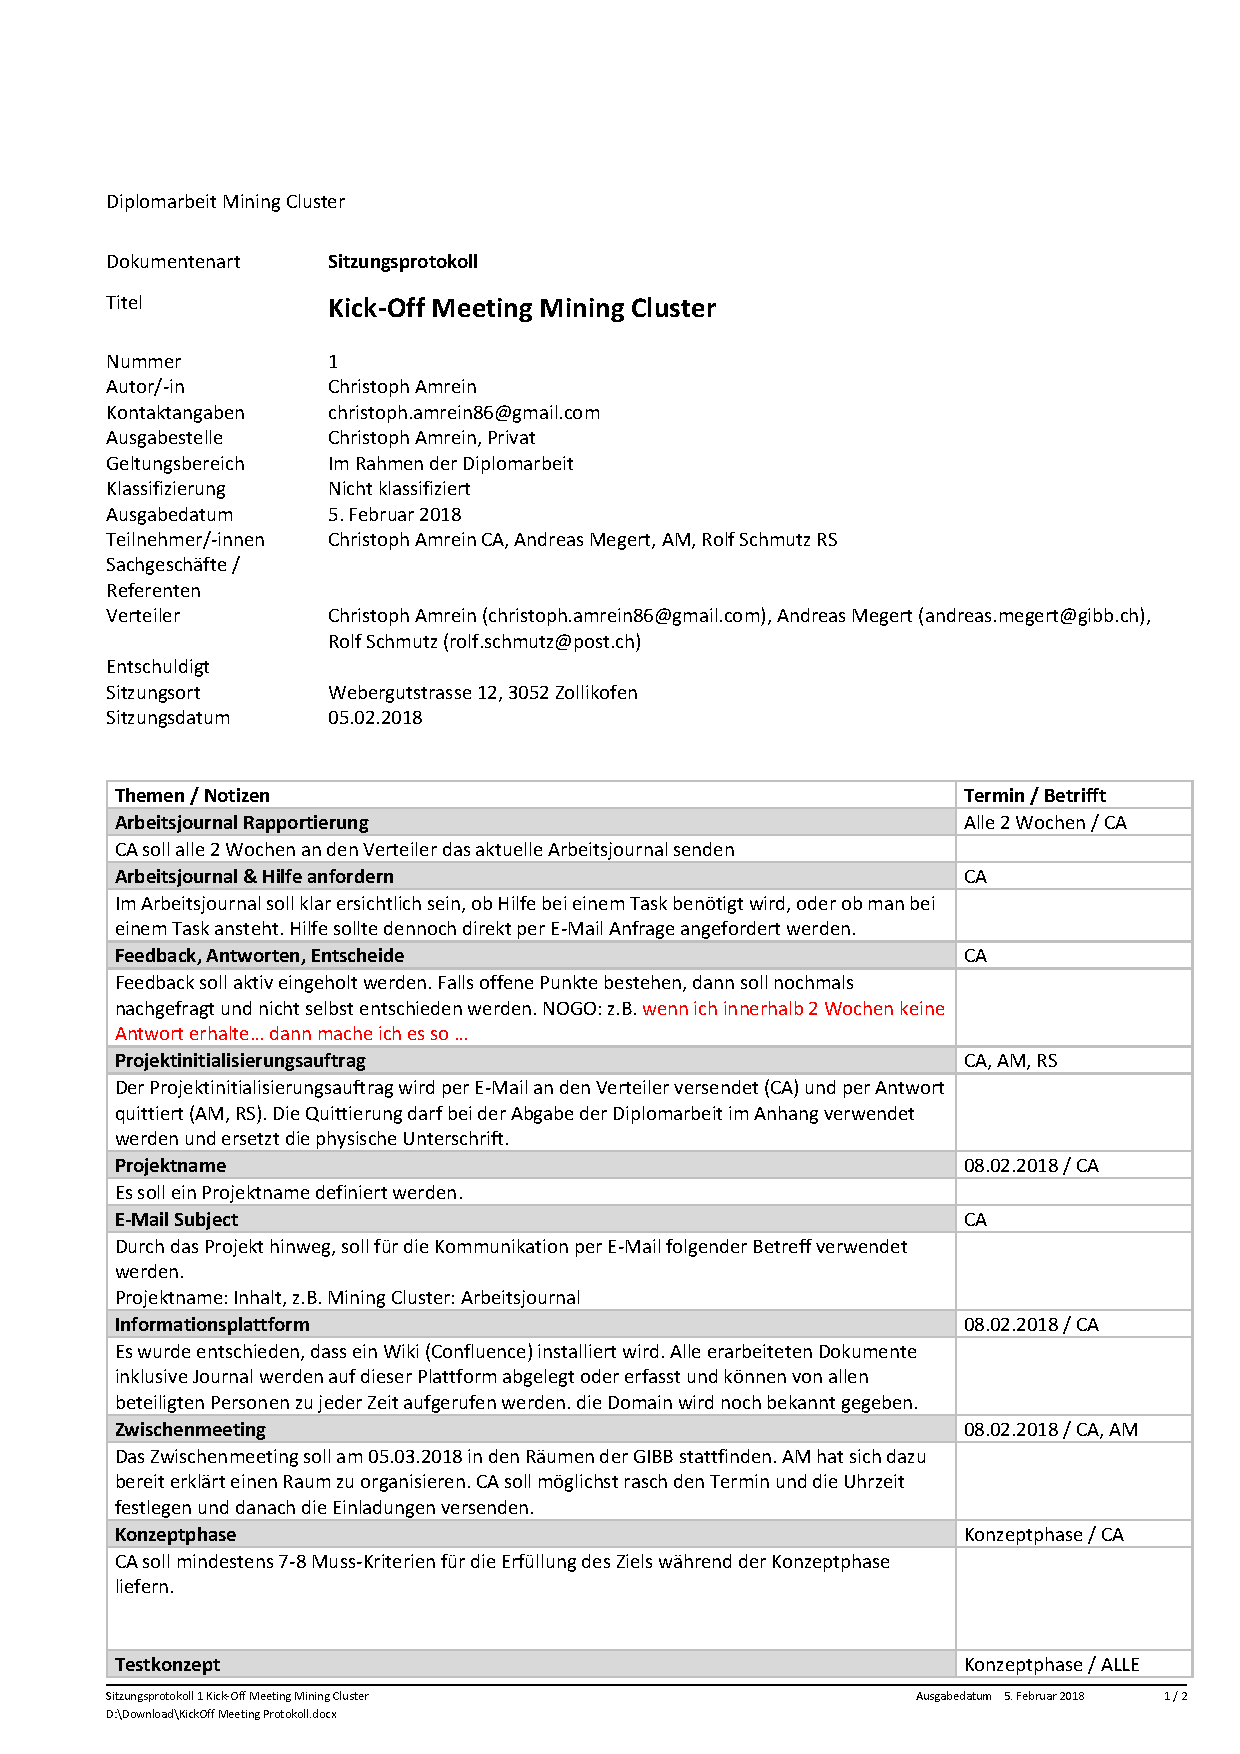
\includepdf[pages=1,scale=.8,pagecommand={\section{Protokoll}\label{pdf:KickOff  Meeting Protokoll}},linktodoc=true]{Anhang/KickOffMeetingProtokoll.pdf}
\includepdf[pages={2},scale=0.9,pagecommand={},linktodoc=true]{Anhang/KickOffMeetingProtokoll.pdf}

% !TEX root = ../Diplombericht.tex
\section{Arbeitsjournal}
\begin{longtable}{|p{5cm}|p{5cm}|p{6cm}|}
\hline
\rowcolor{heading}\textbf{Tag:} 1 & \textbf{Datum:} 05.02.2018 & \textbf{Aufwand:} \\ \hline
\textbf{Erledigte Arbeit} & \multicolumn{2}{p{11cm}|}{- Es wurde ein Share für die Ablage der entstehenden Dokumente und Arbeiten erstellt \newline
- Projektinitialisierungsauftrag wurde geschrieben \newline
- Kick-Off Meeting geplant und durchgeführt} \\ \hline
\textbf{Aufgetretene Probleme} & \multicolumn{2}{p{11cm}|}{-} \\ \hline
\rowcolor{heading}\textbf{Tag:} 2 & \textbf{Datum:} 06.02.2018 & \textbf{Aufwand:} \\ \hline
\textbf{Erledigte Arbeit} & \multicolumn{2}{p{11cm}|}{Confluence für das Projekt eingerichtet (Wurde am Kick-Off Meeting entschieden) \newline
- Protokoll des Kick-Off Meetings verfeinert \newline
- Projektinitialisierungsauftrag gemäss Feedback aus Kick-Off Meeting angepasst \newline
- Projektnamen definiert \newline
- Beginn mit der Projektplanung} \\ \hline
\textbf{Aufgetretene Probleme} & \multicolumn{2}{p{11cm}|}{-} \\ \hline
\rowcolor{heading}\textbf{Tag:} 3 & \textbf{Datum:} 07.02.2018 & \textbf{Aufwand:} \\ \hline
\textbf{Erledigte Arbeit} & \multicolumn{2}{p{11cm}|}{- Zusammenfassung des Kick-Off Meetings an die Anwesenden versendet \newline
- Administrative Arbeiten (Organisation)} \\ \hline
\textbf{Aufgetretene Probleme} & \multicolumn{2}{p{11cm}|}{-} \\ \hline
\rowcolor{heading}\textbf{Tag:} 4 & \textbf{Datum:} 08.02.2018 & \textbf{Aufwand:} \\ \hline
\textbf{Erledigte Arbeit} & \multicolumn{2}{p{11cm}|}{- An der Projektplanung gearbeitet} \\ \hline
\textbf{Aufgetretene Probleme} & \multicolumn{2}{p{11cm}|}{-} \\ \hline
\rowcolor{heading}\textbf{Tag:} 5 & \textbf{Datum:} 09.02.2018 & \textbf{Aufwand:} \\ \hline
\textbf{Erledigte Arbeit} & \multicolumn{2}{p{11cm}|}{-} \\ \hline
\textbf{Aufgetretene Probleme} & \multicolumn{2}{p{11cm}|}{-} \\ \hline
\rowcolor{heading}\textbf{Tag:} 6 & \textbf{Datum:} 10.02.2018 & \textbf{Aufwand:} \\ \hline
\textbf{Erledigte Arbeit} & \multicolumn{2}{p{11cm}|}{-} \\ \hline
\textbf{Aufgetretene Probleme} & \multicolumn{2}{p{11cm}|}{-} \\ \hline
\rowcolor{heading}\textbf{Tag:} 7 & \textbf{Datum:} 11.02.2018 & \textbf{Aufwand:} \\ \hline
\textbf{Erledigte Arbeit} & \multicolumn{2}{p{11cm}|}{-} \\ \hline
\textbf{Aufgetretene Probleme} & \multicolumn{2}{p{11cm}|}{-} \\ \hline
\rowcolor{heading}\textbf{Tag:} 8 & \textbf{Datum:} 12.02.2018 & \textbf{Aufwand:} \\ \hline
\textbf{Erledigte Arbeit} & \multicolumn{2}{p{11cm}|}{- Terminplan und Projektübersicht im Confluence erstellen \newline
- An der Projektplanung weitergearbeitet \newline
- Beginn mit dem Projektauftrag} \\ \hline
\textbf{Aufgetretene Probleme} & \multicolumn{2}{p{11cm}|}{-} \\ \hline
\rowcolor{heading}\textbf{Tag:} 9 & \textbf{Datum:} 13.02.2018 & \textbf{Aufwand:} \\ \hline
\textbf{Erledigte Arbeit} & \multicolumn{2}{p{11cm}|}{- Am Projektauftrag weitergearbeitet} \\ \hline
\textbf{Aufgetretene Probleme} & \multicolumn{2}{p{11cm}|}{-} \\ \hline
\rowcolor{heading}\textbf{Tag:} 10 & \textbf{Datum:} 14.02.2018 & \textbf{Aufwand:} \\ \hline
\textbf{Erledigte Arbeit} & \multicolumn{2}{p{11cm}|}{-} \\ \hline
\textbf{Aufgetretene Probleme} & \multicolumn{2}{p{11cm}|}{-} \\ \hline
\rowcolor{heading}\textbf{Tag:} 11 & \textbf{Datum:} 15.02.2018 & \textbf{Aufwand:} \\ \hline
\textbf{Erledigte Arbeit} & \multicolumn{2}{p{11cm}|}{- Projektauftrag fertiggestellt \newline
- Administrative Arbeiten} \\ \hline
\textbf{Aufgetretene Probleme} & \multicolumn{2}{p{11cm}|}{-} \\ \hline
\rowcolor{heading}\textbf{Tag:} 12 & \textbf{Datum:} 16.02.2018 & \textbf{Aufwand:} \\ \hline
\textbf{Erledigte Arbeit} & \multicolumn{2}{p{11cm}|}{- Krank} \\ \hline
\textbf{Aufgetretene Probleme} & \multicolumn{2}{p{11cm}|}{-} \\ \hline
\rowcolor{heading}\textbf{Tag:} 13 & \textbf{Datum:} 17.02.2018 & \textbf{Aufwand:} \\ \hline
\textbf{Erledigte Arbeit} & \multicolumn{2}{p{11cm}|}{- Krank} \\ \hline
\textbf{Aufgetretene Probleme} & \multicolumn{2}{p{11cm}|}{-} \\ \hline
\rowcolor{heading}\textbf{Tag:} 14 & \textbf{Datum:} 18.02.2018 & \textbf{Aufwand:} \\ \hline
\textbf{Erledigte Arbeit} & \multicolumn{2}{p{11cm}|}{- Krank} \\ \hline
\textbf{Aufgetretene Probleme} & \multicolumn{2}{p{11cm}|}{-} \\ \hline
\rowcolor{heading}\textbf{Tag:} 15 & \textbf{Datum:} 19.02.2018 & \textbf{Aufwand:} \\ \hline
\textbf{Erledigte Arbeit} & \multicolumn{2}{p{11cm}|}{- Krank} \\ \hline
\textbf{Aufgetretene Probleme} & \multicolumn{2}{p{11cm}|}{-} \\ \hline
\rowcolor{heading}\textbf{Tag:} 16 & \textbf{Datum:} 20.02.2018 & \textbf{Aufwand:} \\ \hline
\textbf{Erledigte Arbeit} & \multicolumn{2}{p{11cm}|}{- Krank} \\ \hline
\textbf{Aufgetretene Probleme} & \multicolumn{2}{p{11cm}|}{-} \\ \hline
\rowcolor{heading}\textbf{Tag:} 17 & \textbf{Datum:} 21.02.2018 & \textbf{Aufwand:} \\ \hline
\textbf{Erledigte Arbeit} & \multicolumn{2}{p{11cm}|}{- Krank} \\ \hline
\textbf{Aufgetretene Probleme} & \multicolumn{2}{p{11cm}|}{-} \\ \hline
\rowcolor{heading}\textbf{Tag:} 18 & \textbf{Datum:} 22.02.2018 & \textbf{Aufwand:} \\ \hline
\textbf{Erledigte Arbeit} & \multicolumn{2}{p{11cm}|}{- Krank} \\ \hline
\textbf{Aufgetretene Probleme} & \multicolumn{2}{p{11cm}|}{-} \\ \hline
\rowcolor{heading}\textbf{Tag:} 19 & \textbf{Datum:} 23.02.2018 & \textbf{Aufwand:} \\ \hline
\textbf{Erledigte Arbeit} & \multicolumn{2}{p{11cm}|}{- Krank} \\ \hline
\textbf{Aufgetretene Probleme} & \multicolumn{2}{p{11cm}|}{-} \\ \hline
\rowcolor{heading}\textbf{Tag:} 20 & \textbf{Datum:} 24.02.2018 & \textbf{Aufwand:} \\ \hline
\textbf{Erledigte Arbeit} & \multicolumn{2}{p{11cm}|}{- Krank \newline
- Mit der Studie begonnen \newline
- Informationsbeschaffung der Varianten} \\ \hline
\textbf{Aufgetretene Probleme} & \multicolumn{2}{p{11cm}|}{-} \\ \hline
\rowcolor{heading}\textbf{Tag:} 21 & \textbf{Datum:} 25.02.2018 & \textbf{Aufwand:} \\ \hline
\textbf{Erledigte Arbeit} & \multicolumn{2}{p{11cm}|}{- Studie ausarbeiten \newline
- Informationsbeschaffung \newline
- IST Zustand beschreiben \newline
- Ziele beschreiben} \\ \hline
\textbf{Aufgetretene Probleme} & \multicolumn{2}{p{11cm}|}{-} \\ \hline
\rowcolor{heading}\textbf{Tag:} 22 & \textbf{Datum:} 26.02.2018 & \textbf{Aufwand:} \\ \hline
\textbf{Erledigte Arbeit} & \multicolumn{2}{p{11cm}|}{- Studie abschliessen \newline
- Ziele erweitern \newline
- Varianten beschreiben \newline
- Variantenentscheid fällen \newline
- Empfehlung der Variante beschreiben} \\ \hline
\textbf{Aufgetretene Probleme} & \multicolumn{2}{p{11cm}|}{-} \\ \hline
\rowcolor{heading}\textbf{Tag:} 23 & \textbf{Datum:} 27.02.2018 & \textbf{Aufwand:} \\ \hline
\textbf{Erledigte Arbeit} & \multicolumn{2}{p{11cm}|}{- Projektauftrag mit den neuen Erkenntnissen der Studie ergänzen} \\ \hline
\textbf{Aufgetretene Probleme} & \multicolumn{2}{p{11cm}|}{-} \\ \hline
\rowcolor{heading}\textbf{Tag:} 24 & \textbf{Datum:} 28.02.2018 & \textbf{Aufwand:} \\ \hline
\textbf{Erledigte Arbeit} & \multicolumn{2}{p{11cm}|}{- Projektauftrag fertigstellen \newline
- Studie fertigstellen
- Zwischenmeeting vorbereiten} \\ \hline
\textbf{Aufgetretene Probleme} & \multicolumn{2}{p{11cm}|}{Das vorgesehene Zeitkontingent der Studie wurde überschossen} \\ \hline
\rowcolor{heading}\textbf{Tag:} 25 & \textbf{Datum:} 01.03.2018 & \textbf{Aufwand:} \\ \hline
\textbf{Erledigte Arbeit} & \multicolumn{2}{p{11cm}|}{- Zwischenmeeting vorbereiten \newline
- Finale Version Projektauftrag \newline
- Finale Version Studie \newline
- Powerpoint Präsentation (Agenda) erstellen \newline
- Projektplan updaten } \\ \hline
\textbf{Aufgetretene Probleme} & \multicolumn{2}{p{11cm}|}{-} \\ \hline
\rowcolor{heading}\textbf{Tag:} 26 & \textbf{Datum:} 02.03.2018 & \textbf{Aufwand:} \\ \hline
\textbf{Erledigte Arbeit} & \multicolumn{2}{p{11cm}|}{-} \\ \hline
\textbf{Aufgetretene Probleme} & \multicolumn{2}{p{11cm}|}{-} \\ \hline
\rowcolor{heading}\textbf{Tag:} 27 & \textbf{Datum:} 03.03.2018 & \textbf{Aufwand:} \\ \hline
\textbf{Erledigte Arbeit} & \multicolumn{2}{p{11cm}|}{-} \\ \hline
\textbf{Aufgetretene Probleme} & \multicolumn{2}{p{11cm}|}{-} \\ \hline
\rowcolor{heading}\textbf{Tag:} 28 & \textbf{Datum:} 04.03.2018 & \textbf{Aufwand:} \\ \hline
\textbf{Erledigte Arbeit} & \multicolumn{2}{p{11cm}|}{-} \\ \hline
\textbf{Aufgetretene Probleme} & \multicolumn{2}{p{11cm}|}{-} \\ \hline
\rowcolor{heading}\textbf{Tag:} 29 & \textbf{Datum:} 05.03.2018 & \textbf{Aufwand:} \\ \hline
\textbf{Erledigte Arbeit} & \multicolumn{2}{p{11cm}|}{-} \\ \hline
\textbf{Aufgetretene Probleme} & \multicolumn{2}{p{11cm}|}{-} \\ \hline
\rowcolor{heading}\textbf{Tag:} 30 & \textbf{Datum:} 06.03.2018 & \textbf{Aufwand:} \\ \hline
\textbf{Erledigte Arbeit} & \multicolumn{2}{p{11cm}|}{-} \\ \hline
\textbf{Aufgetretene Probleme} & \multicolumn{2}{p{11cm}|}{-} \\ \hline
\rowcolor{heading}\textbf{Tag:} 31 & \textbf{Datum:} 07.03.2018 & \textbf{Aufwand:} \\ \hline
\textbf{Erledigte Arbeit} & \multicolumn{2}{p{11cm}|}{Erneute Informationsbeschaffung. Es sind Probleme bei der Installation der Variante OpenHPC aufgetreten. Als Zwischenlösung habe ich entschieden einen Laptop der keinen AMD Prozessor verwendet zu benutzen, da dort das Produkt einfach installiert werden kann. Die Computenodes sollen aber weiterhin via Raspberry PI betrieben werden} \\ \hline
\textbf{Aufgetretene Probleme} & \multicolumn{2}{p{11cm}|}{Zuwenige Informationen über OpenHPC gesammelt} \\ \hline
\rowcolor{heading}\textbf{Tag:} 32 & \textbf{Datum:} 08.03.2018 & \textbf{Aufwand:} \\ \hline
\textbf{Erledigte Arbeit} & \multicolumn{2}{p{11cm}|}{Hostnamen und IP's definiert und in Konzept aufgenommen} \\ \hline
\textbf{Aufgetretene Probleme} & \multicolumn{2}{p{11cm}|}{-} \\ \hline
\rowcolor{heading}\textbf{Tag:} 33 & \textbf{Datum:} 09.03.2018 & \textbf{Aufwand:} \\ \hline
\textbf{Erledigte Arbeit} & \multicolumn{2}{p{11cm}|}{- Ich habe versucht verschiedene CentOS Images auf die Raspberry PI's zu installieren, keines hat funktioniert. Es wird weiterhin nach einer alternative gesucht} \\ \hline
\textbf{Aufgetretene Probleme} & \multicolumn{2}{p{11cm}|}{CentOS Images können nicht auf Raspberry PI's installiert werden.} \\ \hline
\rowcolor{heading}\textbf{Tag:} 34 & \textbf{Datum:} 10.03.2018 & \textbf{Aufwand:} \\ \hline
\textbf{Erledigte Arbeit} & \multicolumn{2}{p{11cm}|}{- Neudefinition der Hostnamen \newline
- OpenHPC wurde auf einem Laptop installier \newline
- Die MAC Adressen der Nodes wurden noch nicht ausgelesen deshalb können die Computenodes noch nicht dem Cluster zugewiesen werden \newline
- Die Warewulf Komponente funktioniert noch nicht, somit kann das Betriebssystem noch nich auf die Computenodes verteilt werden} \\ \hline
\textbf{Aufgetretene Probleme} & \multicolumn{2}{p{11cm}|}{WareWulf Komponente blockiert die PXE Boot Installation} \\ \hline
\rowcolor{heading}\textbf{Tag:} 35 & \textbf{Datum:} 11.03.2018 & \textbf{Aufwand:} \\ \hline
\textbf{Erledigte Arbeit} & \multicolumn{2}{p{11cm}|}{- 10 MAC Adressen der RPI's ausgelesen, dafür musste ich eine SD Karte welche ein kompatibles OS für die RPI's besitzt verwenden. Danach habe ich über nmap die MAC Adressen jeweils ausgelesen} \\ \hline
\textbf{Aufgetretene Probleme} & \multicolumn{2}{p{11cm}|}{-} \\ \hline
\rowcolor{heading}\textbf{Tag:} 36 & \textbf{Datum:} 12.03.2018 & \textbf{Aufwand:} \\ \hline
\textbf{Erledigte Arbeit} & \multicolumn{2}{p{11cm}|}{- Ich habe mit dem physischen Aufbau des Clusters begonnen. \newline
- Distanzbolzen mit Raspberry PI's verbunden \newline
- Patchkabel and Raspberry PI's und Switch angeschlossen \newline
- Netzteil via Jumper Kabel an Raspberry PI's angeschlossen} \\ \hline
\textbf{Aufgetretene Probleme} & \multicolumn{2}{p{11cm}|}{Die Lösung sieht instabil aus} \\ \hline
\rowcolor{heading}\textbf{Tag:} 37 & \textbf{Datum:} 13.03.2018 & \textbf{Aufwand:} \\ \hline
\textbf{Erledigte Arbeit} & \multicolumn{2}{p{11cm}|}{- Stromtest des Clusters durchgeführt. 24 Stunden lang den Cluster mit Strom versorgt und beobachtet ob am Schluss Raspberry PI's ausgefallen sind. \newline
- Informationen über das Bedienen von OpenHPC eingeholt} \\ \hline
\textbf{Aufgetretene Probleme} & \multicolumn{2}{p{11cm}|}{} \\ \hline
\rowcolor{heading}\textbf{Tag:} 38 & \textbf{Datum:} 14.03.2018 & \textbf{Aufwand:} \\ \hline
\textbf{Erledigte Arbeit} & \multicolumn{2}{p{11cm}|}{- ein weiterer Versuch PXE Boot mit Warewulf umzusetzen. Dabei bin ich auf Informationen gestossen, dass dies mit den ARMv8 Prozessoren aufgrunde der Architektur nicht möglich ist} \\ \hline
\textbf{Aufgetretene Probleme} & \multicolumn{2}{p{11cm}|}{Warewulf ist nicht mit Raspberry PI's kompatibel} \\ \hline
\rowcolor{heading}\textbf{Tag:} 39 & \textbf{Datum:} 15.03.2018 & \textbf{Aufwand:} \\ \hline
\textbf{Erledigte Arbeit} & \multicolumn{2}{p{11cm}|}{- Weitere Versuche PXE Boot mit Warewulf einzurichten, da ich es nicht glauben kann, dass dies nicht gehen soll} \\ \hline
\textbf{Aufgetretene Probleme} & \multicolumn{2}{p{11cm}|}{Warewulf ist nicht mit Raspberry PI's kompatibel} \\ \hline
\rowcolor{heading}\textbf{Tag:} 40 & \textbf{Datum:} 16.03.2018 & \textbf{Aufwand:} \\ \hline
\textbf{Erledigte Arbeit} & \multicolumn{2}{p{11cm}|}{- Weitere Versuche PXE Boot mit Warewulf einzurichten, da ich es nicht glauben kann, dass dies nicht gehen soll} \\ \hline
\textbf{Aufgetretene Probleme} & \multicolumn{2}{p{11cm}|}{Warewulf ist nicht mit Raspberry PI's kompatibel} \\ \hline
\rowcolor{heading}\textbf{Tag:} 41 & \textbf{Datum:} 17.03.2018 & \textbf{Aufwand:} \\ \hline
\textbf{Erledigte Arbeit} & \multicolumn{2}{p{11cm}|}{- Weitere Versuche PXE Boot mit Warewulf einzurichten, da ich es nicht glauben kann, dass dies nicht gehen soll} \\ \hline
\textbf{Aufgetretene Probleme} & \multicolumn{2}{p{11cm}|}{Warewulf ist nicht mit Raspberry PI's kompatibel} \\ \hline
\rowcolor{heading}\textbf{Tag:} 42 & \textbf{Datum:} 18.03.2018 & \textbf{Aufwand:} \\ \hline
\textbf{Erledigte Arbeit} & \multicolumn{2}{p{11cm}|}{- Den PXE Boot mit einem NOOBS Betriebssystem aufgesetzt. Dies hat funktioniert \newline
- Dies habe ich versucht in Warewulf zu implementieren. Leider erfolglos \newline
Entschieden den TFTBOOT / PXE ohne WareWulf auf dem Managementnode einzurichten.} \\ \hline
\textbf{Aufgetretene Probleme} & \multicolumn{2}{p{11cm}|}{} \\ \hline
\rowcolor{heading}\textbf{Tag:} 43 & \textbf{Datum:} 19.03.2018 & \textbf{Aufwand:} \\ \hline
\textbf{Erledigte Arbeit} & \multicolumn{2}{p{11cm}|}{- Installationsscript geschrieben, welches alles automatisch installiert} \\ \hline
\textbf{Aufgetretene Probleme} & \multicolumn{2}{p{11cm}|}{Es bestehen noch Probleme mit der Installation von CentOS auf den Raspberry PI's} \\ \hline
\rowcolor{heading}\textbf{Tag:} 44 & \textbf{Datum:} 20.03.2018 & \textbf{Aufwand:} \\ \hline
\textbf{Erledigte Arbeit} & \multicolumn{2}{p{11cm}|}{- Den Managementnode mehrfach neu aufgesetzt \newline
- Weitere Abklärungen betreffend, PXE, CentOS und Warewulf} \\ \hline
\textbf{Aufgetretene Probleme} & \multicolumn{2}{p{11cm}|}{} \\ \hline
\rowcolor{heading}\textbf{Tag:} 45 & \textbf{Datum:} 21.03.2018 & \textbf{Aufwand:} \\ \hline
\textbf{Erledigte Arbeit} & \multicolumn{2}{p{11cm}|}{- Ich habe versucht diverse Images auf die SD Karte zu schreiben und die Raspberry PI's zu betreiben \newline
- Die Images stammen von \url{http://mirror.centos.org/altarch/7/isos/aarch64/}} \\ \hline
\textbf{Aufgetretene Probleme} & \multicolumn{2}{p{11cm}|}{- Leider hat kein Image funktioniert \newline
- Vermutlich kann der Kernel nicht richtig geladen werden oder ist nicht kompatibel} \\ \hline
\rowcolor{heading}\textbf{Tag:} 46 & \textbf{Datum:} 22.03.2018 & \textbf{Aufwand:} \\ \hline
\textbf{Erledigte Arbeit} & \multicolumn{2}{p{11cm}|}{- Weitere fremde Images versucht zu installieren, z.B. Gentoo 64 Bit für Raspberry PI's, Fedora, usw.} \\ \hline
\textbf{Aufgetretene Probleme} & \multicolumn{2}{p{11cm}|}{-} \\ \hline
\rowcolor{heading}\textbf{Tag:} 47 & \textbf{Datum:} 23.03.2018 & \textbf{Aufwand:} \\ \hline
\textbf{Erledigte Arbeit} & \multicolumn{2}{p{11cm}|}{- Ich habe nach einer alternativen 64 Bit Version für RPI's gesucht. Dabei bin ich auf diverse Images gestossen: \newline Fedora \url{https://fedoraproject.org/wiki/Architectures/ARM}, die Installation hat einwandfrei funktioniert. (CentOS nahe) \newline Gentoo https://github.com/sakaki-/gentoo-on-rpi3-64bit, die Installation haut auf anhieb funktioniert. Ich bin auf diesen Guide gestossen: \url{https://github.com/umiddelb/aarch64/wiki/Install-CentOS-7-on-your-favourite-ARMv8-ARM64-AArch64-board}, durch diesen Guide habe ich den Durchbruch geschafft. Die Installation habe ich mit der Fedora Boot Partition leider nicht geschafft, mit der Gentoo Lösung ging es aber. Ich bin dabei wie folgt vorgegangen: Beim Schreiben des Gentoo Images auf die SD Karte, werden zwei Partitionen erstellt (Boot \& FileSystem). Die Boot Partition habe ich nicht angepasst. Wichtig dabei ist, dass das RPI ein Kernel8.img für ARMv8 in der Boot Partition benötigt. Dies musste ich also stehen lassen. Als zweiten Schritt habe ich aus dem CentOS Repos das Archiv CentOS-7-aarch64-rootfs-7.4.1708.tar.xz heruntergeladen. Darin ist das komplette FileSystem enthalten. Dies habe ich auf der FileSystem Partition mit dem Befehl tar --numeric-owner -xpJf .../CentOS-7-aarch64-rootfs-7.4.1708.tar.xz -C /home/camrein/Downloads/mnt2 niedergschrieben. (Achtung die Partition wurde nach /home/camrein/Downloads/mnt2 gemountet) Danach hatte ich ein funktionsfaehiges CentOS 64 Bit auf dem Raspberry PI} \\ \hline
\textbf{Aufgetretene Probleme} & \multicolumn{2}{p{11cm}|}{-} \\ \hline
\rowcolor{heading}\textbf{Tag:} 48 & \textbf{Datum:} 24.03.2018 & \textbf{Aufwand:} \\ \hline
\textbf{Erledigte Arbeit} & \multicolumn{2}{p{11cm}|}{- 	
Das Das CentOS nun erfolgreich auf dem RPI betrieben werden kann, habe ich versucht in RPI als Management Node zu verwenden. Bei der Installation des Provisioning Progammes Warewulf bin ich jeweils auf Fehler gestossen. Leider konnte ich in keinem Log inkl Systemlogs keinen Eintrag zum Fehler finden. Das RPI ist jedoch immer wieder eingefrorern. Deshalb habe ich versucht einen üblichen PXE Boot mit TFT einzurichten. Dies hat einwandfrei funktioniert. Bei jedem Erfolg habe ich die SD Karte erneut kopiert, so dass beim Aufsetzen des RPI's wieder möglichst rasch mit einem stabilen Ausgangspunkt weitergemacht werden kann.} \\ \hline
\textbf{Aufgetretene Probleme} & \multicolumn{2}{p{11cm}|}{- Beim PXE Boot trat ich auf diverse Probleme. Jedoch habe ich durch lesen von mehreren Anleitungen und Guides dies beheben können. Ich hatte nicht alles Dateien von der Boot Partition im entsprechenden tftboot Ordner drin} \\ \hline
\rowcolor{heading}\textbf{Tag:} 49 & \textbf{Datum:} 25.03.2018 & \textbf{Aufwand:} \\ \hline
\textbf{Erledigte Arbeit} & \multicolumn{2}{p{11cm}|}{- Administratives, Dokumente nachführen. Entscheidungen treffen. Ich habe mich entschieden es nochmals mit dem Laptop als Managementnode zu versuchen. Dieser hat einen Intel Prozessor und Warewulf kann ohne Probleme auf dem Managementnode installiert werden. Ich habe mich dazu entschlossen als nächsten Schritt es nochmals zu versuchen das vorhandene tftboot Image in Warewulf zu implementieren. Dies würde die Installation enorm vereinfachen, da die Raspberry PI's direkt über die MAC Adresse eine IP und einen Hostnamen zugewiesen werden.} \\ \hline
\textbf{Aufgetretene Probleme} & \multicolumn{2}{p{11cm}|}{-} \\ \hline
\rowcolor{heading}\textbf{Tag:} 50 & \textbf{Datum:} 26.03.2018 & \textbf{Aufwand:} \\ \hline
\textbf{Erledigte Arbeit} & \multicolumn{2}{p{11cm}|}{- Zur Erkenntnis genommen, das die MS Office Tools für mich nicht zu gebrauchen sind. Ich habe mich entschieden die Dokumentation mit LaTeX zu schreiben} \\ \hline
\textbf{Aufgetretene Probleme} & \multicolumn{2}{p{11cm}|}{-} \\ \hline
\rowcolor{heading}\textbf{Tag:} 51 & \textbf{Datum:} 27.03.2018 & \textbf{Aufwand:} \\ \hline
\textbf{Erledigte Arbeit} & \multicolumn{2}{p{11cm}|}{- Studieren von LaTeX: Ich habe noch nie mit LaTeX gearbeitet, es begeistert mich aber, deshalb habe ich mir Beispiele von Dokumentationen und Befehlen angeschaut} \\ \hline
\textbf{Aufgetretene Probleme} & \multicolumn{2}{p{11cm}|}{-} \\ \hline
\rowcolor{heading}\textbf{Tag:} 52 & \textbf{Datum:} 28.03.2018 & \textbf{Aufwand:} \\ \hline
\textbf{Erledigte Arbeit} & \multicolumn{2}{p{11cm}|}{- Versuche mit LaTeX: Ich habe versucht selbst ein LaTeX Dokument zu erstellen und mich mit Freunden darüber unterhalten, dabei habe ich erfahren, dass es bereits sehr gute vordefinierte Templates gibt, welche frei im Internet beziehbar sind} \\ \hline
\textbf{Aufgetretene Probleme} & \multicolumn{2}{p{11cm}|}{-} \\ \hline
\rowcolor{heading}\textbf{Tag:} 53 & \textbf{Datum:} 29.03.2018 & \textbf{Aufwand:} \\ \hline
\textbf{Erledigte Arbeit} & \multicolumn{2}{p{11cm}|}{- Ich habe mich für ein LaTeX Template von Macke entschieden und mit der Migration von Word nach LaText begonnen} \\ \hline
\textbf{Aufgetretene Probleme} & \multicolumn{2}{p{11cm}|}{-} \\ \hline
\rowcolor{heading}\textbf{Tag:} 54 & \textbf{Datum:} 30.03.2018 & \textbf{Aufwand:} \\ \hline
\textbf{Erledigte Arbeit} & \multicolumn{2}{p{11cm}|}{- Ausgangslage und Projektziele nach LaTeX migriert} \\ \hline
\textbf{Aufgetretene Probleme} & \multicolumn{2}{p{11cm}|}{-} \\ \hline\rowcolor{heading}\textbf{Tag:} 55 & \textbf{Datum:} 31.03.2018 & \textbf{Aufwand:} \\ \hline
\textbf{Erledigte Arbeit} & \multicolumn{2}{p{11cm}|}{- Termine und Projektorganisation nach LaTeX migriert} \\ \hline
\textbf{Aufgetretene Probleme} & \multicolumn{2}{p{11cm}|}{-} \\ \hline
\rowcolor{heading}\textbf{Tag:} 56 & \textbf{Datum:} 01.04.2018 & \textbf{Aufwand:} \\ \hline
\textbf{Erledigte Arbeit} & \multicolumn{2}{p{11cm}|}{- Überarbeitung der Darstellung der bereits migrierten Inhalte} \\ \hline
\textbf{Aufgetretene Probleme} & \multicolumn{2}{p{11cm}|}{-} \\ \hline
\rowcolor{heading}\textbf{Tag:} 57 & \textbf{Datum:} 02.04.2018 & \textbf{Aufwand:} \\ \hline
\textbf{Erledigte Arbeit} & \multicolumn{2}{p{11cm}|}{- Kapitel Ressourcen nach LaTeX migriert} \\ \hline
\textbf{Aufgetretene Probleme} & \multicolumn{2}{p{11cm}|}{-} \\ \hline
\rowcolor{heading}\textbf{Tag:} 58 & \textbf{Datum:} 03.04.2018 & \textbf{Aufwand:} \\ \hline
\textbf{Erledigte Arbeit} & \multicolumn{2}{p{11cm}|}{- Überarbeitung bisheriger Dokumentation in LaTeX} \\ \hline
\textbf{Aufgetretene Probleme} & \multicolumn{2}{p{11cm}|}{-} \\ \hline
\rowcolor{heading}\textbf{Tag:} 59 & \textbf{Datum:} 04.04.2018 & \textbf{Aufwand:} \\ \hline
\textbf{Erledigte Arbeit} & \multicolumn{2}{p{11cm}|}{- Design Anpassungen des Diplomberichts} \\ \hline
\textbf{Aufgetretene Probleme} & \multicolumn{2}{p{11cm}|}{-} \\ \hline
\rowcolor{heading}\textbf{Tag:} 60 & \textbf{Datum:} 05.04.2018 & \textbf{Aufwand:} \\ \hline
\textbf{Erledigte Arbeit} & \multicolumn{2}{p{11cm}|}{-} \\ \hline
\textbf{Aufgetretene Probleme} & \multicolumn{2}{p{11cm}|}{-} \\ \hline
\rowcolor{heading}\textbf{Tag:} 61 & \textbf{Datum:} 06.04.2018 & \textbf{Aufwand:} \\ \hline
\textbf{Erledigte Arbeit} & \multicolumn{2}{p{11cm}|}{-} \\ \hline
\textbf{Aufgetretene Probleme} & \multicolumn{2}{p{11cm}|}{-} \\ \hline
\rowcolor{heading}\textbf{Tag:} 62 & \textbf{Datum:} 07.04.2018 & \textbf{Aufwand:} \\ \hline
\textbf{Erledigte Arbeit} & \multicolumn{2}{p{11cm}|}{- Abschliessen der Migration des Projektauftrags (LaTeX) \newline -Informationen über OpenHPC Warewulf und ARMv8 sammeln, da ich noch Probleme mit dem Provisioning des Betriebssystems habe.} \\ \hline
\textbf{Aufgetretene Probleme} & \multicolumn{2}{p{11cm}|}{-} \\ \hline
\rowcolor{heading}\textbf{Tag:} 62 & \textbf{Datum:} 08.04.2018 & \textbf{Aufwand:} \\ \hline
\textbf{Erledigte Arbeit} & \multicolumn{2}{p{11cm}|}{- Studie nach LaTex migrieren \newline
- Informationen über OpenHPC Warewulf und ARMv8 sammeln, da ich noch Probleme mit dem Provisioning des Betriebssystems habe} \\ \hline
\textbf{Aufgetretene Probleme} & \multicolumn{2}{p{11cm}|}{-} \\ \hline
\rowcolor{heading}\textbf{Tag:} 63 & \textbf{Datum:} 09.04.2018 & \textbf{Aufwand:} \\ \hline
\textbf{Erledigte Arbeit} & \multicolumn{2}{p{11cm}|}{- Überarbeitung bisheriger Dokumentation und Konzept Dokumentation migrieren.} \\ \hline
\textbf{Aufgetretene Probleme} & \multicolumn{2}{p{11cm}|}{-} \\ \hline
\rowcolor{heading}\textbf{Tag:} 64 & \textbf{Datum:} 10.04.2018 & \textbf{Aufwand:} \\ \hline
\textbf{Erledigte Arbeit} & \multicolumn{2}{p{11cm}|}{- Entschieden Warewulf auszulassen und mit dnsmasq und pxe boot fortzufahren. PXE Boot mit Centos eingerichtet, alle Raspberry PI's können gestartet werden und beziehen das Betriebssystem über das Netzwerk} \\ \hline
\textbf{Aufgetretene Probleme} & \multicolumn{2}{p{11cm}|}{-} \\ \hline
\rowcolor{heading}\textbf{Tag:} 65 & \textbf{Datum:} 11.04.2018 & \textbf{Aufwand:} \\ \hline
\textbf{Erledigte Arbeit} & \multicolumn{2}{p{11cm}|}{- Nagios einrichten. Es existiert ein Bug mit Centos 7.4. der Ordner /var/run/nagios wird nicht automatisch erstellt. Debuggen bislang erfolglos. Wenn ich in der Konfiguration ein anderes Verzeichnis für die PID Ablage erstelle funktioniert dies noch nicht. Standard Monitoring für alle Nodes eingerichtet. Es müssen aber noch spezifiziertere Überwachungen geschrieben werden} \\ \hline
\textbf{Aufgetretene Probleme} & \multicolumn{2}{p{11cm}|}{-} \\ \hline
\rowcolor{heading}\textbf{Tag:} 66 & \textbf{Datum:} 12.04.2018 & \textbf{Aufwand:} \\ \hline
\textbf{Erledigte Arbeit} & \multicolumn{2}{p{11cm}|}{- Installationsskript anpassen und updaten. Ich habe eine Kopie der SD Karte erstellt. Die SD Karte wurde danach gelöscht und ich habe mit dem automatisierten Installationsskript den Cluster wieder versucht zu installieren. Dabei sind folgende Probleme noch vorhanden: \newline - NTP Sync von Master zu Computenodes \newline
- Slurmd startet nicht automatisch auf den Computes \newline 
- Nagios PID Fehler \newline 
- Ganglia Errors in /var/log/messages ( Keine Nodes werden aufgeführt)} \\ \hline
\textbf{Aufgetretene Probleme} & \multicolumn{2}{p{11cm}|}{-} \\ \hline
\rowcolor{heading}\textbf{Tag:} 67 & \textbf{Datum:} 13.04.2018 & \textbf{Aufwand:} \\ \hline
\textbf{Erledigte Arbeit} & \multicolumn{2}{p{11cm}|}{- Slurm Konfiguration manuell angepasst. Fehler gefunden und behoben. Versucht ersten Job zu erstellen. Jedoch noch erfolglos.} \\ \hline
\textbf{Aufgetretene Probleme} & \multicolumn{2}{p{11cm}|}{- Jobs können in Slurm nocht nicht erstellt werden} \\ \hline
\rowcolor{heading}\textbf{Tag:} 68 & \textbf{Datum:} 14.04.2018 & \textbf{Aufwand:} \\ \hline
\textbf{Erledigte Arbeit} & \multicolumn{2}{p{11cm}|}{- Herausgefunden wie Jobs erstellt werden müssen. Anstatt ein sbatch Script muss mit dem Befehl srun gearbeitet werden. Job erstellt und einen Testlauf vollzogen} \\ \hline
\textbf{Aufgetretene Probleme} & \multicolumn{2}{p{11cm}|}{-} \\ \hline
\rowcolor{heading}\textbf{Tag:} 69 & \textbf{Datum:} 15.04.2018 & \textbf{Aufwand:} \\ \hline
\textbf{Erledigte Arbeit} & \multicolumn{2}{p{11cm}|}{- Dokumentation nachgeführt} \\ \hline
\textbf{Aufgetretene Probleme} & \multicolumn{2}{p{11cm}|}{-} \\ \hline
\rowcolor{heading}\textbf{Tag:} 70 & \textbf{Datum:} 16.04.2018 & \textbf{Aufwand:} \\ \hline
\textbf{Erledigte Arbeit} & \multicolumn{2}{p{11cm}|}{- Bei einem erneuten Testlauf ist ein Raspberry PI beschädigt worden. Ich wollte es austauschen und habe Bemerkt das der Aufwand für den Austausch zu viel Zeit kostet. Deshalb habe ich nochmals den Aufbau überdacht. \newline 
- Dokumentation nachführen, Heatsinks installieren} \\ \hline
\textbf{Aufgetretene Probleme} & \multicolumn{2}{p{11cm}|}{-} \\ \hline
\rowcolor{heading}\textbf{Tag:} 71 & \textbf{Datum:} 17.04.2018 & \textbf{Aufwand:} \\ \hline
\textbf{Erledigte Arbeit} & \multicolumn{2}{p{11cm}|}{- Neuen Aufbau des Clusters in Angriff genommen. Ich habe mir ein passendes Gerüst / Gestell in einem Warenhaus gekauft. } \\ \hline
\textbf{Aufgetretene Probleme} & \multicolumn{2}{p{11cm}|}{-} \\ \hline
\rowcolor{heading}\textbf{Tag:} 72 & \textbf{Datum:} 18.04.2018 & \textbf{Aufwand:} \\ \hline
\textbf{Erledigte Arbeit} & \multicolumn{2}{p{11cm}|}{- Schrauben für die Montage der Raspberry PI's bestellt \newline
- Dokumentation nachgeführt.} \\ \hline
\textbf{Aufgetretene Probleme} & \multicolumn{2}{p{11cm}|}{-} \\ \hline
\rowcolor{heading}\textbf{Tag:} 73 & \textbf{Datum:} 19.04.2018 & \textbf{Aufwand:} \\ \hline
\textbf{Erledigte Arbeit} & \multicolumn{2}{p{11cm}|}{- Überarbeitung des Diplomberichts} \\ \hline
\textbf{Aufgetretene Probleme} & \multicolumn{2}{p{11cm}|}{-} \\ \hline
\rowcolor{heading}\textbf{Tag:} 74 & \textbf{Datum:} 20.04.2018 & \textbf{Aufwand:} \\ \hline
\textbf{Erledigte Arbeit} & \multicolumn{2}{p{11cm}|}{- Diplombericht erweitern} \\ \hline
\textbf{Aufgetretene Probleme} & \multicolumn{2}{p{11cm}|}{-} \\ \hline
\rowcolor{heading}\textbf{Tag:} 75 & \textbf{Datum:} 21.04.2018 & \textbf{Aufwand:} \\ \hline
\textbf{Erledigte Arbeit} & \multicolumn{2}{p{11cm}|}{- Diplombericht erweitern} \\ \hline
\textbf{Aufgetretene Probleme} & \multicolumn{2}{p{11cm}|}{-} \\ \hline
\rowcolor{heading}\textbf{Tag:} 76 & \textbf{Datum:} 22.04.2018 & \textbf{Aufwand:} \\ \hline
\textbf{Erledigte Arbeit} & \multicolumn{2}{p{11cm}|}{- Diplombericht erweitern} \\ \hline
\textbf{Aufgetretene Probleme} & \multicolumn{2}{p{11cm}|}{-} \\ \hline
\rowcolor{heading}\textbf{Tag:} 77 & \textbf{Datum:} 23.04.2018 & \textbf{Aufwand:} \\ \hline
\textbf{Erledigte Arbeit} & \multicolumn{2}{p{11cm}|}{- Schrauben sind angekommen.\newline
- Ich habe den Cluster neu zusammengestellt.} \\ \hline
\textbf{Aufgetretene Probleme} & \multicolumn{2}{p{11cm}|}{-} \\ \hline
\rowcolor{heading}\textbf{Tag:} 78 & \textbf{Datum:} 24.04.2018 & \textbf{Aufwand:} \\ \hline
\textbf{Erledigte Arbeit} & \multicolumn{2}{p{11cm}|}{- Wackelkontakte waren vorhanden. Ich musste nochmals die Verkabelung stabiler gestalten. Die Raspberry PI's wurden nicht konstant mit 5 Volt versorgt} \\ \hline
\textbf{Aufgetretene Probleme} & \multicolumn{2}{p{11cm}|}{-} \\ \hline
\rowcolor{heading}\textbf{Tag:} 79 & \textbf{Datum:} 25.04.2018 & \textbf{Aufwand:} \\ \hline
\textbf{Erledigte Arbeit} & \multicolumn{2}{p{11cm}|}{-} \\ \hline
\textbf{Aufgetretene Probleme} & \multicolumn{2}{p{11cm}|}{-} \\ \hline
\rowcolor{heading}\textbf{Tag:} 80 & \textbf{Datum:} 26.04.2018 & \textbf{Aufwand:} \\ \hline
\textbf{Erledigte Arbeit} & \multicolumn{2}{p{11cm}|}{- Dokumentation erweitert} \\ \hline
\textbf{Aufgetretene Probleme} & \multicolumn{2}{p{11cm}|}{-} \\ \hline
\rowcolor{heading}\textbf{Tag:} 81 & \textbf{Datum:} 27.04.2018 & \textbf{Aufwand:} \\ \hline
\textbf{Erledigte Arbeit} & \multicolumn{2}{p{11cm}|}{- Monitoring Programme optimieren und einrichten. Nagios konnte auf nicht alle Ports eine Verbindung aufbauen. Dies wurde gefixt. Die Ursprüngliche Konfiguration war nicht für die Umgebung eingerichtet} \\ \hline
\textbf{Aufgetretene Probleme} & \multicolumn{2}{p{11cm}|}{-} \\ \hline
\rowcolor{heading}\textbf{Tag:} 82 & \textbf{Datum:} 28.04.2018 & \textbf{Aufwand:} \\ \hline
\textbf{Erledigte Arbeit} & \multicolumn{2}{p{11cm}|}{-} \\ \hline
\textbf{Aufgetretene Probleme} & \multicolumn{2}{p{11cm}|}{-} \\ \hline
\rowcolor{heading}\textbf{Tag:} 83 & \textbf{Datum:} 29.04.2018 & \textbf{Aufwand:} \\ \hline
\textbf{Erledigte Arbeit} & \multicolumn{2}{p{11cm}|}{-} \\ \hline
\textbf{Aufgetretene Probleme} & \multicolumn{2}{p{11cm}|}{-} \\ \hline
\rowcolor{heading}\textbf{Tag:} 84 & \textbf{Datum:} 30.04.2018 & \textbf{Aufwand:} \\ \hline
\textbf{Erledigte Arbeit} & \multicolumn{2}{p{11cm}|}{- Ganglia Monitoring konfiguriert, XMLParser Fehler waren vorhanden. Ganglia wurde für RPI Tests optimiert} \\ \hline
\textbf{Aufgetretene Probleme} & \multicolumn{2}{p{11cm}|}{-} \\ \hline
\rowcolor{heading}\textbf{Tag:} 85 & \textbf{Datum:} 01.05.2018 & \textbf{Aufwand:} \\ \hline
\textbf{Erledigte Arbeit} & \multicolumn{2}{p{11cm}|}{- Mining Tests absolviert. Alle gewünschten Währungen wurden für eine Testdauer von jeweils 30 Minuten geschürft \newline
- Die Raspberry PI's müssen noch übertaktet werden} \\ \hline
\textbf{Aufgetretene Probleme} & \multicolumn{2}{p{11cm}|}{-} \\ \hline
\rowcolor{heading}\textbf{Tag:} 86 & \textbf{Datum:} 02.05.2018 & \textbf{Aufwand:} \\ \hline
\textbf{Erledigte Arbeit} & \multicolumn{2}{p{11cm}|}{- Dokumentation nachgerführt \newline
- Raspberry PI's übertaktet (PXE Boot Image)} \\ \hline
\textbf{Aufgetretene Probleme} & \multicolumn{2}{p{11cm}|}{-} \\ \hline
\rowcolor{heading}\textbf{Tag:} 87 & \textbf{Datum:} 03.05.2018 & \textbf{Aufwand:} \\ \hline
\textbf{Erledigte Arbeit} & \multicolumn{2}{p{11cm}|}{- Dokumentation erweitert} \\ \hline
\textbf{Aufgetretene Probleme} & \multicolumn{2}{p{11cm}|}{-} \\ \hline
\rowcolor{heading}\textbf{Tag:} 88 & \textbf{Datum:} 04.05.2018 & \textbf{Aufwand:} \\ \hline
\textbf{Erledigte Arbeit} & \multicolumn{2}{p{11cm}|}{- Dokumentation erweitert} \\ \hline
\textbf{Aufgetretene Probleme} & \multicolumn{2}{p{11cm}|}{-} \\ \hline
\rowcolor{heading}\textbf{Tag:} 89 & \textbf{Datum:} 05.05.2018 & \textbf{Aufwand:} \\ \hline
\textbf{Erledigte Arbeit} & \multicolumn{2}{p{11cm}|}{-} \\ \hline
\textbf{Aufgetretene Probleme} & \multicolumn{2}{p{11cm}|}{-} \\ \hline
\rowcolor{heading}\textbf{Tag:} 90 & \textbf{Datum:} 06.05.2018 & \textbf{Aufwand:} \\ \hline
\textbf{Erledigte Arbeit} & \multicolumn{2}{p{11cm}|}{-} \\ \hline
\textbf{Aufgetretene Probleme} & \multicolumn{2}{p{11cm}|}{-} \\ \hline
\rowcolor{heading}\textbf{Tag:} 91 & \textbf{Datum:} 07.05.2018 & \textbf{Aufwand:} \\ \hline
\textbf{Erledigte Arbeit} & \multicolumn{2}{p{11cm}|}{-} \\ \hline
\textbf{Aufgetretene Probleme} & \multicolumn{2}{p{11cm}|}{-} \\ \hline
\rowcolor{heading}\textbf{Tag:} 92 & \textbf{Datum:} 08.05.2018 & \textbf{Aufwand:} \\ \hline
\textbf{Erledigte Arbeit} & \multicolumn{2}{p{11cm}|}{- Dokumentation erweitert} \\ \hline
\textbf{Aufgetretene Probleme} & \multicolumn{2}{p{11cm}|}{-} \\ \hline
\rowcolor{heading}\textbf{Tag:} 93 & \textbf{Datum:} 09.05.2018 & \textbf{Aufwand:} \\ \hline
\textbf{Erledigte Arbeit} & \multicolumn{2}{p{11cm}|}{- Dokumentation erweitert} \\ \hline
\textbf{Aufgetretene Probleme} & \multicolumn{2}{p{11cm}|}{-} \\ \hline
\rowcolor{heading}\textbf{Tag:} 94 & \textbf{Datum:} 10.05.2018 & \textbf{Aufwand:} \\ \hline
\textbf{Erledigte Arbeit} & \multicolumn{2}{p{11cm}|}{- Dokumentation erweitert} \\ \hline
\textbf{Aufgetretene Probleme} & \multicolumn{2}{p{11cm}|}{-} \\ \hline
\rowcolor{heading}\textbf{Tag:} 95 & \textbf{Datum:} 11.05.2018 & \textbf{Aufwand:} \\ \hline
\textbf{Erledigte Arbeit} & \multicolumn{2}{p{11cm}|}{- Dokumentation erweitert} \\ \hline
\textbf{Aufgetretene Probleme} & \multicolumn{2}{p{11cm}|}{-} \\ \hline
\rowcolor{heading}\textbf{Tag:} 96 & \textbf{Datum:} 12.05.2018 & \textbf{Aufwand:} \\ \hline
\textbf{Erledigte Arbeit} & \multicolumn{2}{p{11cm}|}{- Dokumentation erweitert} \\ \hline
\textbf{Aufgetretene Probleme} & \multicolumn{2}{p{11cm}|}{-} \\ \hline
\rowcolor{heading}\textbf{Tag:} 97 & \textbf{Datum:} 13.05.2018 & \textbf{Aufwand:} \\ \hline
\textbf{Erledigte Arbeit} & \multicolumn{2}{p{11cm}|}{- Dokumentation erweitert} \\ \hline
\textbf{Aufgetretene Probleme} & \multicolumn{2}{p{11cm}|}{-} \\ \hline
\rowcolor{heading}\textbf{Tag:} 98 & \textbf{Datum:} 14.05.2018 & \textbf{Aufwand:} \\ \hline
\textbf{Erledigte Arbeit} & \multicolumn{2}{p{11cm}|}{- Dokumentation erweitert} \\ \hline
\textbf{Aufgetretene Probleme} & \multicolumn{2}{p{11cm}|}{-} \\ \hline
\rowcolor{heading}\textbf{Tag:} 99 & \textbf{Datum:} 15.05.2018 & \textbf{Aufwand:} \\ \hline
\textbf{Erledigte Arbeit} & \multicolumn{2}{p{11cm}|}{- Dokumentation erweitert} \\ \hline
\textbf{Aufgetretene Probleme} & \multicolumn{2}{p{11cm}|}{-} \\ \hline
\rowcolor{heading}\textbf{Tag:} 100 & \textbf{Datum:} 16.05.2018 & \textbf{Aufwand:} \\ \hline
\textbf{Erledigte Arbeit} & \multicolumn{2}{p{11cm}|}{- Dokumentation erweitert} \\ \hline
\textbf{Aufgetretene Probleme} & \multicolumn{2}{p{11cm}|}{-} \\ \hline
\rowcolor{heading}\textbf{Tag:} 101 & \textbf{Datum:} 17.05.2018 & \textbf{Aufwand:} \\ \hline
\textbf{Erledigte Arbeit} & \multicolumn{2}{p{11cm}|}{- Dokumentation erweitert} \\ \hline
\textbf{Aufgetretene Probleme} & \multicolumn{2}{p{11cm}|}{-} \\ \hline
\rowcolor{heading}\textbf{Tag:} 102 & \textbf{Datum:} 18.05.2018 & \textbf{Aufwand:} \\ \hline
\textbf{Erledigte Arbeit} & \multicolumn{2}{p{11cm}|}{- Dokumentation erweitert} \\ \hline
\textbf{Aufgetretene Probleme} & \multicolumn{2}{p{11cm}|}{-} \\ \hline
\rowcolor{heading}\textbf{Tag:} 103 & \textbf{Datum:} 19.05.2018 & \textbf{Aufwand:} \\ \hline
\textbf{Erledigte Arbeit} & \multicolumn{2}{p{11cm}|}{- Dokumentation erweitert} \\ \hline
\textbf{Aufgetretene Probleme} & \multicolumn{2}{p{11cm}|}{-} \\ \hline
\rowcolor{heading}\textbf{Tag:} 104 & \textbf{Datum:} 20.05.2018 & \textbf{Aufwand:} \\ \hline
\textbf{Erledigte Arbeit} & \multicolumn{2}{p{11cm}|}{- Dokumentation abgeschlossen \newline
- Die Dokumentation ist nun bereit für Korrekturen} \\ \hline
\textbf{Aufgetretene Probleme} & \multicolumn{2}{p{11cm}|}{-} \\ \hline
\rowcolor{heading}\textbf{Tag:} 105 & \textbf{Datum:} 21.05.2018 & \textbf{Aufwand:} \\ \hline
\textbf{Erledigte Arbeit} & \multicolumn{2}{p{11cm}|}{- Überarbeitung der Dokumentation} \\ \hline
\textbf{Aufgetretene Probleme} & \multicolumn{2}{p{11cm}|}{-} \\ \hline
\caption{Arbeitsjournal}\\
\end{longtable}


 

% !TEX root = ../Diplombericht.tex
\addcontentsline{toc}{section}{Quellenverzeichnis}
\section*{Quellenverzeichnis}
\begin{table}[H]
\begin{tabular}[t]{p{10cm}|p{6cm}}
\hline
\rowcolor{heading} \textbf{Namen der Quelle} & \textbf{Titel und Bemerkung} \\\hline
\textbf{Wikipedia} \newline
\url{https://en.wikipedia.org/wiki/Comparison\_of\_cluster\_software} & Cluster Software Vergleichstabelle  \\\hline
\textbf{HPC Today} \newline
\url{http://www.hpctoday.com/best-practices/tinytitan-a-raspberry-pi-computing-based-cluster/} & Installationsanleitung und Beschreibung der HPC Lösung TinyTitan  \\\hline
\textbf{Jordi Corbilla von Thundax Software} \newline
\url{http://thundaxsoftware.blogspot.ch/2016/07/creating-raspberry-pi-3-cluster.html} & Komplette Installationsanleitung einer Noname Cluster Lösung \\\hline
\textbf{Benutzer Sakaki auf Github} \newline
\url{https://github.com/sakaki-/gentoo-on-rpi3-64bit} & Repository des Gentoo Images und Installationsanleitung \\\hline
\textbf{CentOS} \newline
\url{http://mirror.centos.org/altarch/7.4.1708/isos/aarch64/} & Image Repository von CentOS \\\hline
\textbf{raspberrypi.org} \newline
\url{https://www.raspberrypi.org/documentation/hardware/raspberrypi/bootmodes/net_tutorial.md} & Installationsanleitung zu PXE / Netzwerkboot \\\hline
\textbf{Fedora} \newline
\url{https://fedoraproject.org/wiki/Architectures/ARM} & Fedora Image für Raspberry PI's und Installationsanleitung dazu \\\hline
\textbf{Benutzer Uli Middelberg auf Github} \newline
\url{https://github.com/umiddelb/aarch64/wiki/Install-CentOS-7-on-your-favourite-ARMv8-ARM64-AArch64-board} & Beschreibung und Anleitung der Umgehungslösung für die Installation von CentOS auf den Raspberry PI's\\\hline
\end{tabular}
\caption{Quellenverzeichnis}
\end{table}
 

\phantomsection
\listoffigures
\cleardoublepage

\phantomsection
\listoftables
\cleardoublepage

\end{document}
